% Masters/Doctoral Thesis 
% LaTeX Template
% Version 2.5 (27/8/17)
%
% This template was downloaded from:
% http://www.LaTeXTemplates.com
%
% Version 2.x major modifications by:
% Vel (vel@latextemplates.com)
%
% This template is based on a template by:
% Steve Gunn (http://users.ecs.soton.ac.uk/srg/softwaretools/document/templates/)
% Sunil Patel (http://www.sunilpatel.co.uk/thesis-template/)
%
% Template license:
% CC BY-NC-SA 3.0 (http://creativecommons.org/licenses/by-nc-sa/3.0/)
%
%%%%%%%%%%%%%%%%%%%%%%%%%%%%%%%%%%%%%%%%%

 
%----------------------------------------------------------------------------------------
%	PACKAGES AND OTHER DOCUMENT CONFIGURATIONS
%----------------------------------------------------------------------------------------

\documentclass[
12pt, % The default document font size, options: 10pt, 11pt, 12pt
% oneside, % Two side (alternating margins) for binding by default, uncomment to switch to one side
english, % ngerman for German
singlespacing, % Single line spacing, alternatives: onehalfspacing or doublespacing
liststotoc, % Uncomment to add the list of figures/tables/etc to the table of contents
% toctotoc, % Uncomment to add the main table of contents to the table of contents
% parskip, % Uncomment to add space between paragraphs
headsepline, % Uncomment to get a line under the header
% consistentlayout, % Uncomment to change the layout of the declaration, abstract and acknowledgements pages to match the default layout
]{MastersDoctoralThesis} % The class file specifying the document structure

\usepackage[utf8]{inputenc}  % required for inputting international characters
\usepackage[T1]{fontenc}  % output font encoding for international characters
\usepackage{amsmath, amsfonts, amssymb}  % all the good math stuff
\usepackage{bm}  % bold symbols in math mode
\usepackage{tikz}  % create and include Tikz figures
\usepackage[autostyle=true]{csquotes}  % required to generate language-dependent quotes in the bibliography
\usepackage{caption}     % this and below are used for the
\usepackage{subcaption}  % subfigures throughout the document
\usepackage{siunitx}  % good macros for SI units
% \usepackage{annotate-equations}  % not sure I use this
\usepackage{tabularray}  % holy grail of tables
% \usepackage{thumbs}  % add thumbs to the sides of pages
\usepackage{titlesec}  % to style chapter titles
\usepackage[bibstyle=numeric, citestyle=numeric-comp, sorting=none]{biblatex}  % the only good way to do citations and bibliography
\usepackage[colorlinks=true, allcolors=blue]{hyperref}  % hyperlinks through the document
\usepackage[xcolor,notion]{knowledge}  % define notions to be linked to inside the document | load after hyperref
\usepackage[capitalise, nameinlink]{cleveref}  % get smart references across the document | load last!
% \usepackage{microtype}  % improves the spacing between words and letters, only include in last stages of compilation, takes time!

% \usepackage{utopia}  % Use the Palatino font
% \usepackage{newtxtext,newtxmath}  % Use the TeX Gyre Termes font
\usepackage{tgheros}  % Use the TeX Gyre Heros font
\usetikzlibrary{matrix}
\UseTblrLibrary{amsmath}  % Makes tabularray load amsmath and register better environments
\setcounter{secnumdepth}{3}
\addbibresource{Bibliography.bib}

% ----- Defining Colors Used Later ----- %
\definecolor{wpblue}{RGB}{0, 0, 245}
\definecolor{wpred}{RGB}{234, 51, 36}
\definecolor{latwiss_blue}{RGB}{163, 178, 234}
\definecolor{latwiss_red}{RGB}{238, 134, 131}
\definecolor{latwiss_yellow}{RGB}{228, 202, 135}
\definecolor{latwiss_green}{RGB}{155, 194, 148}

%----------------------------------------------------------------------------------------
%	SIUNITX SETTINGS
%----------------------------------------------------------------------------------------

\sisetup{
    exponent-product=\times,      % operator between number and 10^n
    print-unity-mantissa=false,  % no 1 x 10^3, only 10^3
    % inter-unit-product=\cdot,
    % separate-uncertainty,
    % table-align-uncertainty,
}

%----------------------------------------------------------------------------------------
%	MARGIN SETTINGS
%----------------------------------------------------------------------------------------

\geometry{
	paper=a4paper, % Change to letterpaper for US letter
	inner=2.5cm, % Inner margin
	outer=2.5cm, % Outer margin
	bindingoffset=.5cm, % Binding offset
	top=1.5cm, % Top margin
	bottom=1.5cm, % Bottom margin
	% showframe, % Uncomment to show how the type block is set on the page
}


%----------------------------------------------------------------------------------------
%	THESIS INFORMATION
%----------------------------------------------------------------------------------------

\thesistitle{Local Interaction Region Coupling Correction for the LHC} % Print with \ttitle
\supervisor{Prof. Carsten \textsc{Welsch}} % Print with \supname
\examiner{} % Print with \examname
\degree{Doctor of Philosophy} % Print with \degreename
\author{Felix \textsc{Soubelet}} % Print with \authorname
\addresses{} % Print with \addressname
\subject{Accelerator Physics} % Print with \subjectname
\keywords{} % Print with \keywordnames
\university{\href{https://www.liverpool.ac.uk/}{University of Liverpool}} % Print with \univname
\department{\href{https://www.liverpool.ac.uk/physical-sciences/}{School of Physical Sciences}} % Print with \deptname
\group{\href{https://www.liverpool.ac.uk/quasar/}{QUASAR Group}} % Print with \groupname
\faculty{\href{http://home.cern}{CERN}} % Print with \facname


%----------------------------------------------------------------------------------------
%	START OF DOCUMENT - FRONTMATTER
%----------------------------------------------------------------------------------------

\begin{document}

\frontmatter % Use roman page numbering style (i, ii, iii, iv...) for the pre-content pages

\pagestyle{plain} % Default to the plain heading style until the thesis style is called for the body content

\begin{titlepage}
\begin{center}

\vspace*{.06\textheight}
\vspace{1cm}
{\scshape\LARGE \univname\par} % University name
\vspace{0.8cm}

\begin{figure}[ht]
    \centering
    
\includegraphics[width=\textwidth]{Figures/Logos/UoLlogo.eps}
\end{figure}

\HRule \\[0.4cm] % Horizontal line
{\huge \bfseries \ttitle\par}\vspace{0.4cm} % Thesis title
\HRule \\[1cm] % Horizontal line

\vspace{1cm}

\begin{minipage}[t]{0.4\textwidth}
\begin{flushleft} \large
\text{Submitted by:}\\
\href{https://orcid.org/my-orcid?orcid=0000-0001-8012-1440}{\authorname} % Author name - remove the \href bracket to remove the link
\end{flushleft}
\end{minipage}
\begin{minipage}[t]{0.4\textwidth}
\begin{flushright} \large
\text{Supervised by:}\\
\href{https://www.researchgate.net/profile/Tobias-Persson}{Dr. Tobias~\textsc{Persson}}\\
\href{https://orcid.org/0000-0002-9857-1703}{Dr. Rogelio~\textsc{Tomás}}\\
\href{https://orcid.org/0000-0002-5410-7706}{Dr. Oznur~\textsc{Apsimon}}\\
\href{https://orcid.org/0000-0001-7085-0973}{\supname}\\
\end{flushright}
\end{minipage}

\vspace{1.5cm}

\vfill

\large {Thesis submitted in accordance with the requirements of the\\}
\univname, \deptname \\
\large {for the degree of Doctor in Philosophy}

\vfill

{\large \today}\\[4.5cm] % Date

\vfill
\end{center}
\end{titlepage}
% ----- Commands for recurrent expressions ----- %

% Command for asterisks
\newcommand{\asterisk}{\(^{\ast}\) }  % needs the trailing space


% ----- Commands for recurrent expressions in math mode ----- %

% Command for the absolute value of something
\newcommand{\abs}[1]{\left\lvert #1 \right\rvert}

% Command for the complex conjugate of something
\newcommand{\conj}[1]{#1^{\ast}}

%-----------------------------%
%	     USER COMMANDS        %
%-----------------------------%

% Mark some text as todo, in red
\newcommand{\todo}[1]{\textcolor{red}{TODO: #1}}

% Used for listing of code developments
\newcommand{\ilparagraph}[2]{\paragraph{\textbf{#1}~{#2}\textbf{.}}}
% \dedicatory{For/Dedicated to/To my\ldots}
% \begin{abstract}

In order to further expand our knowledge of the structure of matter and the workings of our universe, scientists are constantly seeking to collide particles at ever-increasing energies and with higher \gls{luminosity}.
So is the task of the \gls{LHC} at \acrshort{CERN}, the highest energy particle accelerator and collider to date, and the goal of its future upgrade into the \gls{HL-LHC}.
This constant progress in performance requires more intense beams and smaller beam sizes at collisions points as well as a tight control of these parameters.
Thus, successful operation of large-scale particle colliders heavily depends on the precise correction of magnet field or alignment errors present in the machine.

In the \gls{LHC}, transverse \gls{betatron_coupling} has been shown to have a significant impact on both the beam dynamics and luminosity production due to uncompensated sources close to the \glspl{IP}.
However, current measurement methods are not sufficient for precise local coupling measurement at the \gls{IP}, and the impact of these sources has so far been left uncompensated.
This thesis covers work done in an effort to determine and correct Interaction Region (\acrshort{IR}) local coupling.

A key tool presented in this document is the designed \gls{RWS}, a new optics configuration which allows the determination of local coupling corrections based on correlated global variables such as the closest tune approach \glssymbol{Cminus}.
The validity of this new method has been demonstrated through simulations and experimental measurements taken during the \gls{LHC} \Gls{run}~\num{3} commissioning in~\num{2022}, where determined corrections were applied and led to a measured luminosity increase of \qty{9.7}{\percent} and \qty{3.5}{\percent} at the \acrshort{ATLAS} and \acrshort{CMS} detectors, respectively.
Additionally, the application of machine learning techniques for high complexity problems such as the detection of coupling sources in the \gls{LHC} \acrshortpl{IR} has been explored, yielding promising results but requiring some more improvements to be operationally viable.
Finally, optics studies which revealed avenues for improvements in the optics measurements done at the LHC are also presented.

\end{abstract}

\glsresetall                                     % reset glossary entries counts for the next chapter

% \begin{declaration}
\addchaptertocentry{\authorshipname} % Add the declaration to the table of contents

\vspace{1cm}

I, \authorname, declare that this thesis and the work presented in it are my own, done while in candidature for a doctorate degree.
This thesis was not used, in whole or in part, to achieve an academic degree.
No external sources were used without declaration in the text: any thoughts from others or literal quotations are clearly marked and where I have quoted from the work of others, the source is always given.
Except for such quotations, this thesis is entirely my own work.\\

Several studies and results presented in this document have already been published, and a summary of these references is given below.
The following articles report on work that was included in this thesis:
\newline \newline
\noindent\cite{IPAC:Soubelet:Prospect_IR_Coupling_Correction_LHC_Run3}: F. Soubelet \textit{et al.}, "Prospects for Local Interaction Region Coupling Correction at the LHC in Run~\num{3}", in Proceedings of \num{12}th Int. Particle Accelerator Conf. (IPAC'21), Campinas, Brazil, MOPAB007, \num{2021}.
\newline \newline
\noindent\cite{IPAC:Soubelet:First_Corrections_IR_Local_Coupling_LHC_Run3}: F. Soubelet \textit{et al.}, "First Interaction Region Local Coupling Corrections in the LHC Run~\num{3}", in Proceedings of \num{13}th Int. Particle Accelerator Conf. (IPAC'22), Bangkok, Thailand, WEPOPT007, \num{2022}.
\newline \newline
\noindent\cite{IPAC:Soubelet:Supervised_Machine_Learning_Local_Coupling_Sources_Detection_LHC}: F. Soubelet \textit{et al.}, "Supervised Machine Learning for Local Coupling Sources Detection in the LHC", in Proceedings of \num{13}th Int. Particle Accelerator Conf. (IPAC'22), Bangkok, Thailand, WEPOPT008, \num{2022}.
\newline \newline
\noindent\todo{PRAB Paper citation}: F. Soubelet \textit{et al.}, "Rigid Waist Shift: A New Method for Local Coupling Corrections in the LHC Interaction Regions", Phys. Rev. Accel. Beams \todo{some number here}, \num{2023}.
\newline \newline
\noindent\todo{IPAC23 Paper citation}: F. Soubelet \textit{et al.}, "Prospect of Operating with Limited Skew Quadrupole Corrector Availability in the LHC Interaction Regions", in Proceedings of \num{14}th Int. Particle Accelerator Conf. (IPAC'23), Venice, Italy, MOPL044, \num{2023}.
\newline
\newline
\indent
The following articles are studies that were contributed to by myself but are not included in this thesis:
\newline \newline
\noindent\cite{IPAC:Tomas:Run2_Experience_View_LHC_HLLHC}: F. Carlier \textit{et al.}, "LHC Run~\num{2} Optics Commissioning Experience in View of HL-LHC", in Proceedings of \num{10}th Int. Particle Accelerator Conf. (IPAC'19), Melbourne, Australia, MOPMP033, \num{2019}.
\newline \newline
\noindent\cite{HPC:Tracey:AI_Holistic}: R. Tracey \textit{et al.}, "AI-Driven Holistic Approach to Energy Efficient HPC", in ISC High Performance \num{2020}: High Performance Computing, pp \num{267}-\num{279}, \num{2020}.
\newline \newline
\noindent\cite{REPORT:Apollinari:HL_LHC_TDR}: I. Béjar Alonso \textit{et al.}, "High-Luminosity Large Hadron Collider (HL-LHC): Technical Design Report", in CERN Yellow Reports: Monographs, \num{2020}.
\newline \newline
\noindent\cite{IPAC:Persson:Optics_Correction_Strategy_2021}: T. Persson \textit{et al.}, "Optics Correction Strategy for Run~\num{3} of the LHC", in Proceedings of \num{12}th Int. Particle Accelerator Conf. (IPAC'21), Campinas, Brazil, WEPAB027, \num{2021}.
\newline \newline
\noindent\cite{IPAC:Maclean:Optics_Measurement_Excitation_Betatron_Oscillations_PSB}: E. Maclean \textit{et al.}, "Optics Measurement by Excitation of Betatron Oscillations in the CERN PSB", in Proceedings of \num{12}th Int. Particle Accelerator Conf. (IPAC'21), Campinas, Brazil, THPAB168, \num{2021}.
\newline \newline
\noindent\cite{IPAC:Persson:Optics_Measurements_Correction_Plans_HLLHC}: T. Persson \textit{et al.}, "Optics Measurements and Correction Plans for the HL-LHC", in Proceedings of \num{12}th Int. Particle Accelerator Conf. (IPAC'21), Campinas, Brazil, WEPAB026, \num{2021}.
\newline \newline
\noindent\cite{REPORT:OMC:Optics_Strategy_HLLHC}: X. Buffat \textit{et al.}, "Optics Measurement and Correction Strategies for HL-LHC", in CERN ATS Notes, \num{2022}. \todo{check later if this is correct}
\newline \newline
\noindent\cite{IPAC:Persson:Optics_Correction_Strategy_2022}: T. Persson \textit{et al.}, "Optics Correction Strategy for Run~\num{3} of the LHC", in Proceedings of \num{13}th Int. Particle Accelerator Conf. (IPAC'22), Bangkok, Thailand, WEPOST008, \num{2022}.
\newline \newline
\noindent\cite{IPAC:Fol:ML_Application_LHC_Optics_Commissioning}: E. Fol \textit{et al.}, "Experimental Demonstration of Machine Learning Application in LHC Optics Commissioning", in Proceedings of \num{13}th Int. Particle Accelerator Conf. (IPAC'22), Bangkok, Thailand, MOPOPT047, \num{2022}.
\newline \newline
\noindent\todo{JOSCH Paper citation}: J. Dilly \textit{et al.}, "First Operational Dodecapole Correction in the LHC", Phys. Rev. Accel. Beams \todo{paper code}, \num{2023}.
\newline \newline
\noindent\todo{IPAC23 Paper citation}: F. Carlier \textit{et al.}, "Prospect of Operating with Limited Skew Quadrupole Corrector Availability in the LHC Interaction Regions", in Proceedings of \num{14}th Int. Particle Accelerator Conf. (IPAC'23), Venice, Italy, MOPL044, \num{2023}.
\newline \newline
\noindent\cite{IPAC:Carlier:Challenges_kmodulation_LHC_Run3}: F. Carlier \textit{et al.}, "Challenges of k-Modulation Measurements in the LHC Run~3", in Proceedings of \num{14}th Int. Particle Accelerator Conf. (IPAC'23), Venice, Italy,  MOPL014, \num{2023}.
\newline \newline
\noindent\cite{IPAC:Carlier:LHC_Run3_Optics_Correction}: F. Carlier \textit{et al.}, "LHC Run~3 Optics Correction", in Proceedings of \num{14}th Int. Particle Accelerator Conf. (IPAC'23), Venice, Italy,  MOPL015, \num{2023}.
\newline \newline
\todo{Check all above and add anything else that I forgot. Also fix the bibtex for IPAC23 papers.}
\end{declaration}

\cleardoublepage
% \begin{acknowledgements}
% \addchaptertocentry{\acknowledgementname} % Add the acknowledgements to the table of contents
\vspace{0.8cm}

% Somehow, this section turned out to be the hardest to write out of this thesis.
Now that the main results of several years of work have been summarized in this little document and, as this writing comes to an end, it is time to look back and thank the many people that have contributed and supported me along the way.
\newline

First and foremost, I wish to thank Tobias Persson with all my heart for his kind supervision and unwavering support during those years.
I consider this PhD to be divided into a before and an after, and you to be the turning point.
I can never thank you enough for your patience, advice, guidance, encouragements and enthusiasm, without which I know I would not have crossed the finish line.
My heartfelt thanks go to Rogelio Tomás as well for keeping my best interest in mind, and for your continuous help and wise feedback throughout.
\newline

A few special people now need to be thanked here.
They have all, each in their own way, significantly contributed to helping me through this long journey.
\newline

A big thanks to Joschua Dilly for your enthusiasm for programming, "clean code" and scientific computing.
Thanks for the reviews, for the late night pull requests, the scientific discussions, the coffees, the control room banter and for your \LaTeX \ black magic knowledge.
This document would not have looked as good without you.

To Félix Carlier, or "Félix number \num{1}", thank you for taking the time to explain so much of the non-linear dynamics theory to me, and for providing advice on the writing of this document.
Your thesis, that you so kindly gave me a physical copy of, has been a great source of inspiration and has set a high standard of quality.

Thank you to Michael Hofer for the countless questions you have answered, for being the first to guide me through the perilous land of Resonance Driving Terms, and for being such an encyclopedia of knowledge and Indico links.

To Elena Fol, thank you for showing me how to teach the machines, for the coffee talks and for being such a little ray of sunshine every day (except when it's cold).

To Axel Poyet, thank you for being you and being there every step of the way, from close and afar.
Thanks for the friendship, the help, the jokes, the sarcasm, the shared struggle and all of the silliest moments: it has been great.

Thank you to Konstantinos Paraschou for being a great flatmate through part of this journey, and getting through the pandemic lockdowns with me: shared mental breakdowns are strangely cathartic.
As you already (don't) know, "book boom".

Thanks also go to my family for their support, patience and encouragements.
\newline

Many other people - so many, actually - have contributed one way or another to this adventure, and a few group mentions are in order.
\newline

My thanks go to all the past and current members of the OMC team for the great work environment of this group, and for their cheerful company during all these hours - mostly nights and weekends - spent in the control room.
I am equally grateful to the LHC Operations team for their collaboration, for accepting me in their midst for a short time, and in particular to Michi Hostettler for being such a source of knowledge and always eager to provide help and advice.
Similar thanks go to the wonderful folks at the IBM Hartree center for taking me in during my placement, especially Vadim Elisseev and Rob Tracey for their close supervision.

Many thanks to some special teachers who have played a bigger part than they know turning me into the scientist I am today: Mr. Bourquard for fostering my curiosity in all things physics-related, and Mr. Beck for helping me find - at my own speed - the beauty in mathematics.
Thank you to Jonathan Ferreira for the passionate and passionating plasma lectures, Alexis Nuttin for equally great neutronics classes; and Elsa Merle-Lucotte for the degree of her involvment helping students find their way.

To all the people I have walked the PhD road with - Thibault, Marie, Eva, Mathilde, Anaïs, Floriane, Guillaume, Mathieu, Nico, Elsa, Élisabeth, Diane, Pauline, Laurène, Émilien, Marouane, Luis and many more - a thousand thanks for your comradeship and the myriad of great moments we have shared.
I wish you to find success and happiness in your journey, wherever it may take you.
\newline

As a final word, a big "thank you!" to all scientists who have advanced this beautiful field of physics, have led to the design, creation and operation of the LHC, and overall have made my PhD possible.
As was put so well into words by Sir Isaac Newton: "If I have seen further, it is by standing on the shoulders of giants."

\end{acknowledgements}
% \newpage
\vspace*{0.4\textheight}
\begin{center}
	\noindent\enquote{\itshape Everything always breaks...}\bigbreak
	Tobias Hakan Bjorn Persson.
\end{center}

\setcounter{tocdepth}{1}  % Determines how detailed the table of content should be
\tableofcontents % Prints the main table of contents
\listoffigures % Prints the list of figures
\listoftables % Prints the list of tables

% \begin{abbreviations}{ll} % Include a list of abbreviations (a table of two columns)

\textbf{ABP}        & CERN's \textbf{A}ccelerators and \textbf{B}eam \textbf{P}hysics group\\
\textbf{AD}         & \textbf{A}ntiproton \textbf{D}ecelerator\\
\textbf{ALICE}      & \textbf{A} \textbf{L}arge \textbf{I}on \textbf{C}ollider \textbf{E}xperiment\\
\textbf{ATLAS}      & \textbf{A} \textbf{T}oroidal \textbf{L}HC \textbf{A}pparatu\textbf{S}\\
\textbf{AWAKE}      & \textbf{A}dvanced \textbf{WAK}efield \textbf{E}xperiment\\
\textbf{BE}         & CERN's \textbf{BE}ams department\\
\textbf{BPM}        & \textbf{B}eam \textbf{P}osition \textbf{M}onitor\\
\textbf{CERN}       & \textbf{E}uropean \textbf{O}rganization for \textbf{N}uclear \textbf{R}esearch\\
\textbf{CMS}        & \textbf{C}ompact \textbf{M}uon \textbf{S}olenoid\\
\textbf{DA}         & \textbf{D}ynamic \textbf{A}perture\\
\textbf{ELENA}      & \textbf{E}xtra \textbf{L}ow \textbf{EN}ergy \textbf{A}ntiproton ring\\
\textbf{HERA}       & \textbf{H}adron-\textbf{E}lectron \textbf{R}ing \textbf{A}ccelerator\\
\textbf{HiRadMat}   & \textbf{H}igh \textbf{Rad}iation to \textbf{Mat}erials\\
\textbf{HL-LHC}     & \textbf{H}igh \textbf{L}uminosity \textbf{L}arge \textbf{H}adron \textbf{C}ollider\\
\textbf{HSS}        & CERN's \textbf{H}adron \textbf{S}ynchrotron \textbf{S}ingle particle effects section\\
\textbf{IP}         & \textbf{I}nteraction \textbf{P}oint\\
\textbf{IR}         & \textbf{I}nteraction \textbf{R}egion\\
\textbf{ISOLDE}     & \textbf{I}sotope \textbf{S}eparator \textbf{O}n \textbf{L}ine \textbf{DE}tector\\
\textbf{LEIR}       & \textbf{L}ow \textbf{E}nergy \textbf{I}on \textbf{R}ing\\
\textbf{LHC}        & \textbf{L}arge \textbf{H}adron \textbf{C}ollider\\
\textbf{LHCb}       & \textbf{L}arge \textbf{H}adron \textbf{C}ollider \textbf{b}eauty\\
\textbf{MAD}        & \textbf{M}ethodical \textbf{A}ccelerator \textbf{D}esign\\
\textbf{n-TOF}      & \textbf{N}eutron \textbf{T}ime \textbf{O}f \textbf{F}light\\
\textbf{OMC}        & \textbf{O}ptics \textbf{M}easurements and \textbf{C}orrections\\
\textbf{PS}         & \textbf{P}roton \textbf{S}ynchrotron\\
\textbf{PTC}        & \textbf{P}olymorphic \textbf{T}racking \textbf{C}ode\\
\textbf{RDT}        & \textbf{R}esonance \textbf{D}riving \textbf{T}erm\\
\textbf{SPS}        & \textbf{S}uper \textbf{P}roton \textbf{S}ynchrotron\\

\end{abbreviations}
% \begin{constants}{lr@{${}={}$}l} % The list of physical constants is a three column table

The \SI{}{} command is provided by the siunitx package, see its documentation for instructions on how to use it

Speed of Light & $c_{0}$ & \SI{2.99792458e8}{\meter\per\second} (exact)\\
Constant Name & $Symbol$ & $Constant Value$ with units\\

\end{constants}
% \begin{symbols}{lll} % Include a list of Symbols (a three column table)

$a$ & distance & \si{\meter} \\
$P$ & power & \si{\watt} (\si{\joule\per\second}) \\
Symbol & Name & Unit \\

\addlinespace % Gap to separate the Roman symbols from the Greek

$\omega$ & angular frequency & \si{\radian} \\

\end{symbols}


%----------------------------------------------------------------------------------------
%	THESIS CONTENT - CHAPTERS
%----------------------------------------------------------------------------------------

\mainmatter % Begin numeric (1,2,3...) page numbering

\pagestyle{thesis} % Return the page headers back to the "thesis" style

%----------------------------------------------------------------------------------------
%	REDEFINE CHAPTER TITLE STYLE
%----------------------------------------------------------------------------------------

% See doc of titlesec page 22 (https://mirror2.sandyriver.net/pub/ctan/macros/latex/contrib/titlesec/titlesec.pdf)
% TODO: fix the slight antisymmetry in vspace bellow CHAPTER N

\titleformat{\chapter}[display]
{\Large\filcenter}
{\titlerule[1pt]%
\vspace{1pt}%
\titlerule
\vspace{1pc}%
\LARGE\MakeUppercase{\chaptertitlename} \thechapter}{1pc}
{\titlerule
\vspace{1pt}%
\titlerule[1pt]%
\vspace{1pc}%
\Huge}
% % Sets the vertical space above and below equations
\setlength{\abovedisplayskip}{15pt}
\setlength{\belowdisplayskip}{15pt}
% \include{Chapters/testchapter.tex}
% \chapter{Introduction}
\label{chapter:introduction}

\begin{noteblock}
    In this document a distinction is made between glossary items and acronyms, and locally relevant terms and concepts.
    The former will appear in \textcolor{cern}{blue} and are clickable links bringing the reader back to the glossary such as the following: \gls{optics}.
    The latter will appear in \concept{orange} and are an indication of a term or concept that is important to the content at hand but does not necessarily warrant its own entry in the glossary.
\end{noteblock}

\section{Motivations}

Accelerator physics as a branch of physics has its roots nearly a century ago with the pioneering work of E.~Lawrence~\cite{PR:Lawrence:Production_High_Speed_Light_Ions} inventing the cyclotron, and shortly after in \num{1932} when J.~Cockcroft and E.~Walton~\cite{LLC:Cockcroft:Disintegration_Lithium_Swift_Protons,TRS:Cockcroft:Experiments_High_Velocity_Positive_Ions_1,TRS:Cockcroft:Experiments_High_Velocity_Positive_Ions_2} built the first particle accelerator that could produce nuclear reactions.
Since then accelerator physics has grown into a mature field of research with applications ranging from cancer treatment and the production of medical isotopes to material science such as the analysis of archeological items, but also many industrial uses.

However, \gls{HEP} - the study of the fundamental constituents of matter - has historically been the main drive to push the boundaries of accelerator science.
Respectively, one of the most significant contributions of this field has been the design, construction and operation of particle colliders providing data for experiments at the forefront of \gls{HEP} research, such as the \gls{LHC} at \acrshort{CERN}, the highest energy and most technologically advanced particle accelerator yet built.
These contributions recently culminated with the discovery of the Higgs boson by the \acrshort{ATLAS} and \acrshort{CMS} experiments at the \acrshort{LHC} in \num{2012}~\cite{PLB:ATLAS:Observation_Higgs_Boson, PLB:CMS:Observation_Higgs_Boson}, which Peter Higgs and François Englert were awarded the \num{2013} Nobel Prize in Physics for theorizing nearly \num{50} years prior~\cite{PRL:Higgs:Broken_Symmetries_Masses_Gauge_Bosons,PRL:Englert:Broken_Symmetry_Mass_Gauge_Vector_Mesons}.

Since then experiments at the \gls{LHC} keep analyzing data from collisions to probe in more details the now uncovered mechanisms, as well as attempt to discover physics beyond the Standard Model such as supersymmetry or dark matter.
To this end, the LHC has kept pushing its performance to even higher energies and \gls{luminosity}.
The machine has already undergone two \glspl{longshutdown} during which it was upgraded, and is currently in the \Gls{run}~\num{3} of its operation.
Another shutdown is planed a few years from now to upgrade the accelerator to the \gls{HL-LHC}~\cite{Website:HLLHC}, which aims to increase the \gls{luminosity} of the collider by a factor of \num{10}.

Increasing the luminosity of the machine however is not without its challenges and limitations, and in order to achieve an optimal performance an understanding and control of the dynamics of the particle beams is essential.
One such limitation to the delivery of optimal \gls{luminosity} is the so-called local linear \gls{betatron_coupling} in the \glspl{IR}, which can lead to a significant decrease in collision numbers if left uncorrected.

The focus of this thesis is on the handling of local linear coupling in the \glspl{IR} of the \gls{LHC}, and the development of a new method to measure and correct the phenomenon, improving the performance of the accelerator.
By addressing this issue, the research presented in this document aims to contribute to the ongoing efforts to push the performance of the \gls{LHC} to even greater heights, and to hopefully enable new discoveries in the field of particle physics.

\section{Thesis Outline}

This document exposes work done on the matter of local linear coupling correction in the LHC, and of this thesis at large.
Across studies a focus is kept on the main \glspl{IR} of the \gls{LHC}, \numlist{1;5}, which are more error-sensitive due to their optics configurations.

As a first step and to allow the reader to follow the details of this work, \cref{chapter:theory} gives a detailed introduction to the world of accelerator physics and beam dynamics.
The chapter starts with the linear beam dynamics as the core foundation to any particle accelerator, then carries on with non-linear phenomenology present in more complex machines in order to introduce necessary concepts and quantities of interest to the work presented in this document, such as \glspl{RDT}.
A section is dedicated to \gls{betatron_coupling} and its parametrization, and another to \gls{luminosity} as a key performance indicator of a collider.

Also in view of helping the reader follows \cref{chapter:lhc_omc} which opens on a comprehensive overview of the \gls{LHC} machine and its operation in \Gls{run}~\num{3}, with particular attention given to the main \glspl{IR}.
The second half of the chapter offers a dive into the practice of \gls{OMC} as done at the \gls{LHC} by the \gls{OMC} team.
Insight is given on each step, going from data acquisition methods and devices to the reconstruction of quantities of interest and the determination of adjustments that would bring the machine closer to its nominal state.

The main body of work for this thesis, which offers a new experimental setup and correction method for local linear coupling in the \gls{LHC} \glspl{IR}, is detailed in \cref{chapter:ir_local_coupling}.
The chapter opens by providing the reader with a justification of the need for local linear coupling correction both for the \gls{LHC} and the future \gls{HL-LHC} machine.
An overview of the local coupling situation in the \gls{LHC} is given, including current correction methods and their limitations which stem from the specific conditions of the \gls{LHC} \glspl{IR}.
The theoretical basis for the new correction method is laid out, which relies on the leakage of \glspl{RDT} from the \glspl{IR} to the rest of the machine, and the various experimental setup tools that were developed are thoroughly presented.
Experimental measurements and data analysis from the method's application in the \gls{LHC} \num{2022} commissioning are presented as well as the resulting \gls{luminosity} improvements observed from the application of the determined corrections.
A short section is dedicated to the relevance of this method for other existing or future colliders.
Finally, the chapter offers an assessment of the realistic eventuality of one or more failure of the dedicated magnets used for coupling correction and the explored solutions.

In line with the themes of the \gls{LIV.DAT}~\cite{Website:LIVDAT} a machine learning based approach to the subject of local linear coupling has been explored, that is presented in \cref{chapter:ml_local_coupling}, which starts with a minimal overview of the relevant machine learning concepts.
The new approach to local linear coupling is presented with a focus on the data preparation, model training and achieved results.
A discussion on the potential of this machine learning approach is held, as well as the challenges to overcome to make it fully viable in \gls{LHC} operations.

Some additional work performed during this thesis is presented in \cref{chapter:others_and_software}.
While not relating directly to the main subject of this thesis, the work presented in this chapter is nonetheless relevant to either the \gls{LHC} and its operation or to the \gls{OMC} team's activities at large.

Finally, \cref{chapter:conclusion} restates the main results and conclusions from the work done in this thesis.
A discussion is held on the findings and any missing element to this work, as well as the potential avenues for future developments.
The chapter closes with a look at the future of LHC operations and potential implications of this work to other colliders.

Some additional material is provided in the appendices of this document.
\Cref{appendix:hamiltonian_derivation} offers a detailed derivation for the Hamiltonian thin kick expansion which would have been too cumbersome to include in \cref{chapter:theory}.
\Cref{appendix:naming_conventions} provides complementary, illustrated supporting material regarding the naming conventions in use for the \gls{LHC}, which the reader might find useful considering the inevitable amount of machine specific jargon used in this document.
In the spirit of completeness, \cref{appendix:experimental_knobs,appendix:inconclusive_measurements,appendix:measurement_fills} provide details on the experimental campaign relating to the studies in this thesis.
The former lists the different experimental knobs used for measurements in the LHC for the results shown in \cref{chapter:ir_local_coupling}, and the latter provides a comprehensive list of the LHC fills used for measurements.
\Cref{appendix:inconclusive_measurements} provides details on additional measurements not presented in detail in \cref{chapter:ir_local_coupling}.
Finally, \cref{appendix:code_developments} succinctly presents the main software development contributions done over the course of this PhD.

\glsresetall                                     % reset glossary entries counts for the next chapter

% \chapter{Theory of Beam Dynamics Relevant to the Large Hadron Collider}

\label{Chapter:Theory} % For referencing the chapter elsewhere, use \cref{Chapter:Theory}

%----------------------------------------------------------------------------------------

The design, operation, performance, and safety of a particle accelerator depend on the study of beam dynamics, a field of accelerator science.
This section provides an overview of the beam dynamics theories relevant to the material in this thesis, and more specifically beam optics.
Most of the material in this section can be found in the literature such as \cite{BOOK:Wilson:Introcution_Particle_Accelerators, BOOK:Lee:Accelerator_physics, BOOK:Wiedemann:Particle_Accelerator_Physics, BOOK:Minty:Measurements_Control_Charged_Particle_Beams,BOOK:Wolski:Beam_dynamics,BOOK:Chao:Handbook_Accelerator_Physics_Engineering, BOOK:Chao:Collective_instabilities}.
When not in these works, explicit references to content are given.
\todo{The chapter starts out with a description of linear dynamics, then moves on to aspects of non-linear dynamics, and ends with a discussion of luminosity}.

%----------------------------------------------------------------------------------------

\section{Linear Beam Dynamics}
\label{section:linear_beam_dynamics}

The linear dynamics of an accelerator are, mainly, the endeavor to bend and focus particle beams to confine them within the machine's aperture.

\subsection{Transport and Guiding of Charged Particles}
\label{subsection:transport_and_guiding_of_charged_particles}

To force the beam's particles into a closed trajectory, they are subjected to magnetic fields that deflect their trajectories.
The force exerted onto the beam is the Lorentz force \(F_{L}\), given by the equation:

\begin{equation}
    \vec{F_L} = \dfrac{d\vec{p}}{dt} = q (\vec{E} + \vec{v} \times \vec{B}) \text{ ,}
    \label{equation:lorentz_force}
\end{equation}
where \(p\) is the particle momentum, \(q\) the particle charge, \(\vec{E}\) the electric field, \(\vec{v}\) the particle velocity and \(\vec{B}\) the magnetic field.
In most accelerators, including the LHC, the particles' speed is close to the celerity of light \(c\) and the force from the magnetic field is significantly stronger than that produced by the electric field for realistic values of \(\vec{E}\) and \(\vec{B}\).
As a result, in high energy particle accelerators magnetic fields are typically used to guide particles.
The guiding magnetic field can be expanded into a series of multipolar fields, for instance here in the horizontal plane:

\begin{align}
    B_{y} = 
    \tikz[baseline]{
        \node[draw=red,rounded corners,anchor=base] (m1)
        {\(\displaystyle B_{y0}\)};
        \node[below of=m1] (l1) {dipole};
        \draw[-,red] (l1) -- (m1);
    }
    +
    \tikz[baseline]{
        \node[draw=red,rounded corners,anchor=base] (m2)
        {\(\displaystyle \frac{dB_{y}}{dx} x\)};
        \node[below of=m2] (l2) {quadrupole};
        \draw[-,red] (l2) -- (m2);
    }
    +
    \tikz[baseline]{
        \node[draw=red,rounded corners,anchor=base] (m3)
        {\(\displaystyle \frac{1}{2!} \frac{d^2B_{y}}{dx^2} x^2\)};
        \node[below of=m3] (l2) {sextupole};
        \draw[-,red] (l2) -- (m3);
    }
    +
    \tikz[baseline]{
        \node[draw=red,rounded corners,anchor=base] (m4)
        {\(\displaystyle \frac{1}{3!} \frac{d^3B_{y}}{dx^3} x^3\)};
        \node[below of=m4] (l2) {octupole};
        \draw[-,red] (l2) -- (m4);
    }
    + \ldots
    \label{equation:magnetic_field_expansion}
\end{align}

Bending forces are supplied by dipole magnets with a magnetic field perpendicular to the beam trajectory, while focusing is typically performed with the use of quadrupole magnets.
Higher orders belong to the nonlinear dynamics and will be discussed later on.
\Cref{figure:frenet_serret_system} illustrates the Frenet-Serret coordinate system traditionally used in linear beam dynamics.

\begin{figure}[!htb]
    \begin{center}
    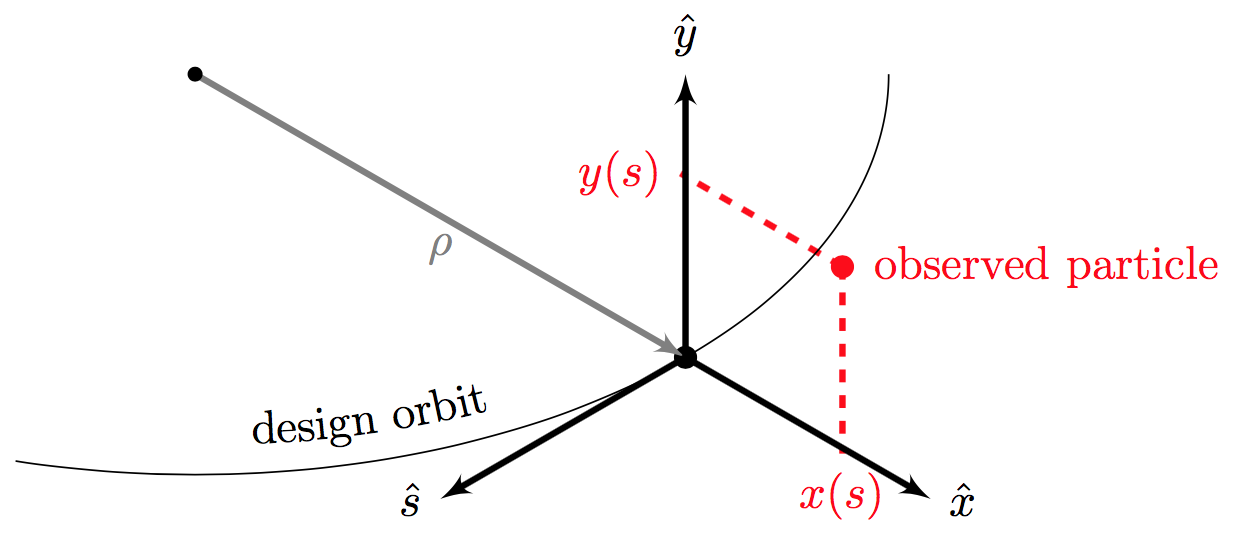
\includegraphics[width = 0.8\linewidth]{Figures/Beam_Dynamics_Theory/Frenet_Serret_Coordinate_System.png}
    \caption{The Frenet-Serret coordinate system used in accelerator physics. Here \(\hat{x}\), \(\hat{y}\), and \(\hat{s}\) form the right-handed orthogonal basis, while \(\rho\) is the local bending radius.}
    \label{figure:frenet_serret_system}
    \end{center}
\end{figure}

The coordinate system travels longitudinally with the particle, along a reference trajectory defined by an ideal, or \intro{synchronous}, particle.
The longitudinal curvilinear coordinate is \(s\), and denotes the position of the particle along the ideal orbit with respect to an arbitrary initial point at \(s = 0\).
One can define a local radius of curvature, \(\rho(s)\), which depends on the local magnetic field \(\vec{B}\) and varies along ring.
The transverse phase space is defined by \((x, x^{\prime}, y, y^{\prime})\), where \(x\) and \(y\) are a particle's coordinates in the transverse plane relative to the reference trajectory.
The \(x^{\prime}\) and \(y^{\prime}\) coordinates are \intro{divergent angles}, with the prime indicating differentiation with respect to \(s\).
\break

In the linear regime, magnetic dipoles define ideal orbit for a particle of \intro{reference momentum} \(p_0\).
This ideal orbit goes through the magnetic center of all elements in the machine to close back on itself after a revolution, and is called a \intro{closed orbit}.
In practice the real closed orbit will deviate from the ideal designed orbit due to various effects such as dipolar field errors.
Particles within the beam are distributed in amplitude and oscillate around the closed orbit, which corresponds to the path of a particle with zero amplitude within the beam, because of focusing forces. 
\break

Focusing forces are typically provided by magnetic quadrupoles: a quadrupolar field acting on a charged particle displaced from the closed orbit will provide a restoring (focusing) force proportional to the displacement in one transverse plane, while simultaneously providing a diverging (defocusing) force in the other. 
As a convention, a quadrupole focusing in the horizontal transverse plane and defocusing in the vertical is referred to as a \intro{focusing quadrupole}. 
Respectively, a quadrupole defocusing in the horizontal plane but focusing in the vertical is referred to as a \intro{defocusing quadrupole}.
A net focusing effect in both planes can be obtained with a setup of quadrupoles of alternating polarity in equal distance, a widely used configuration named the \(\mathrm{FODO}\) cell, a layout alternating quadrupoles in equal distance.
A schematic of a \(\mathrm{FODO}\) cell is shown in \cref{figure:fodo_cell_schematic}.

\begin{figure}[!htb]
    \begin{center}
    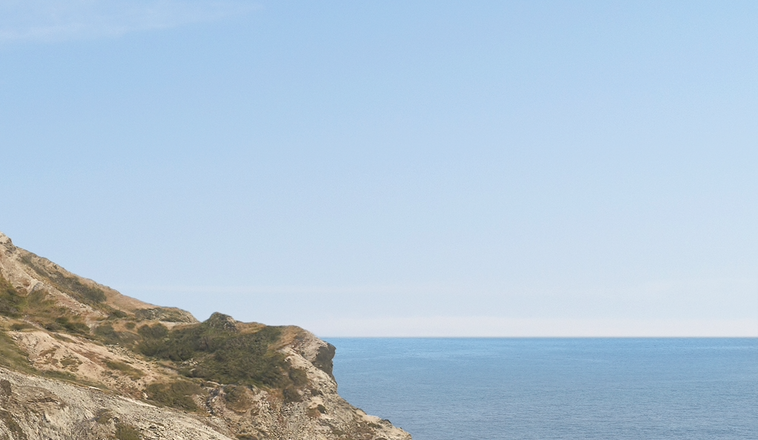
\includegraphics[width = 0.8\linewidth]{Figures/placeholder.png}
    \caption{\todo{Schematic of a \(\mathrm{FODO}\) cell. A focusing quadrupole is denoted with an F while a defocusing one is denoted with a D.}}
    \label{figure:fodo_cell_schematic}
    \end{center}
\end{figure}

For each magnet applying a field \(B\) one can define the \intro{magnetic rigidity}, which is an indication of the field’s ability to alter a particle’s course based on its charge \(q\) and momentum \(p\), as:

\begin{equation}
    B \rho = \frac{p}{q} \text{ .}
    \label{equation:magnetic_rigidity}
\end{equation}

\Cref{figure:dipole_quadrupole_fields} illustrates magnetic fields in an idealized dipole and quadrupole.

\begin{figure}[htp]
    \centering
    \subfloat[.7\linewidth][Ideal dipole.]{
        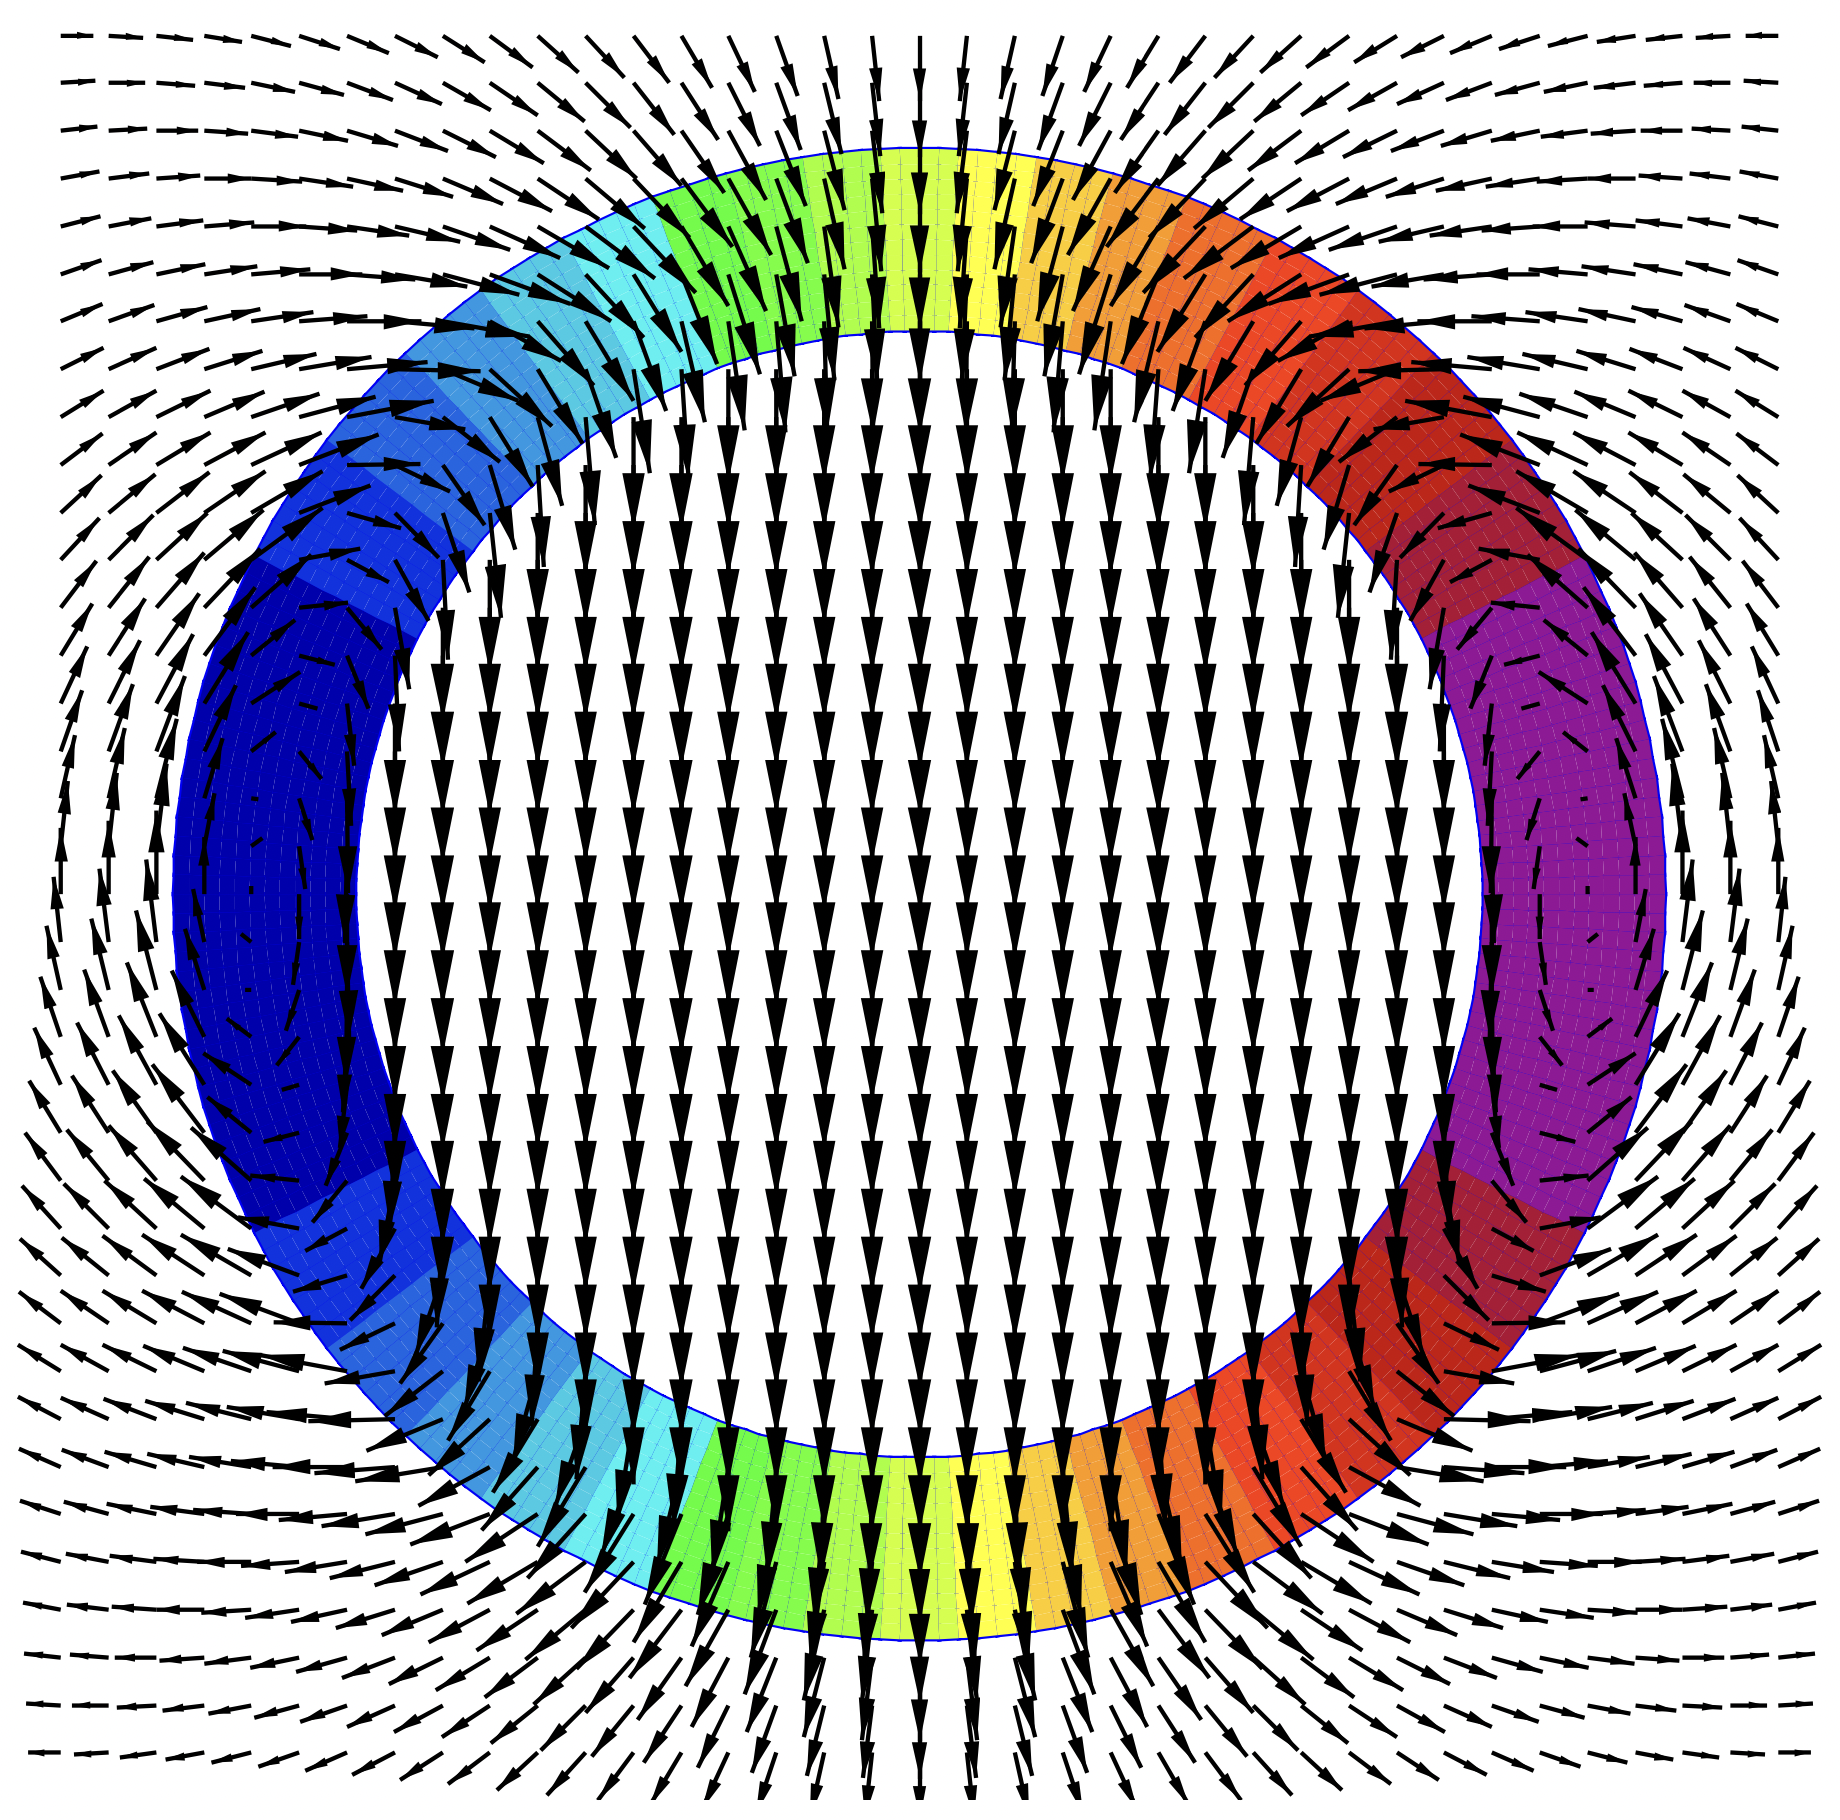
\includegraphics[width=6.5cm]{Figures/Beam_Dynamics_Theory/ideal_dipole_cos_theta.png}
        \label{fig:ideal_dipole}
    }
    \hspace{0.5cm}
    \subfloat[.7\linewidth][Ideal quadrupole.]{
        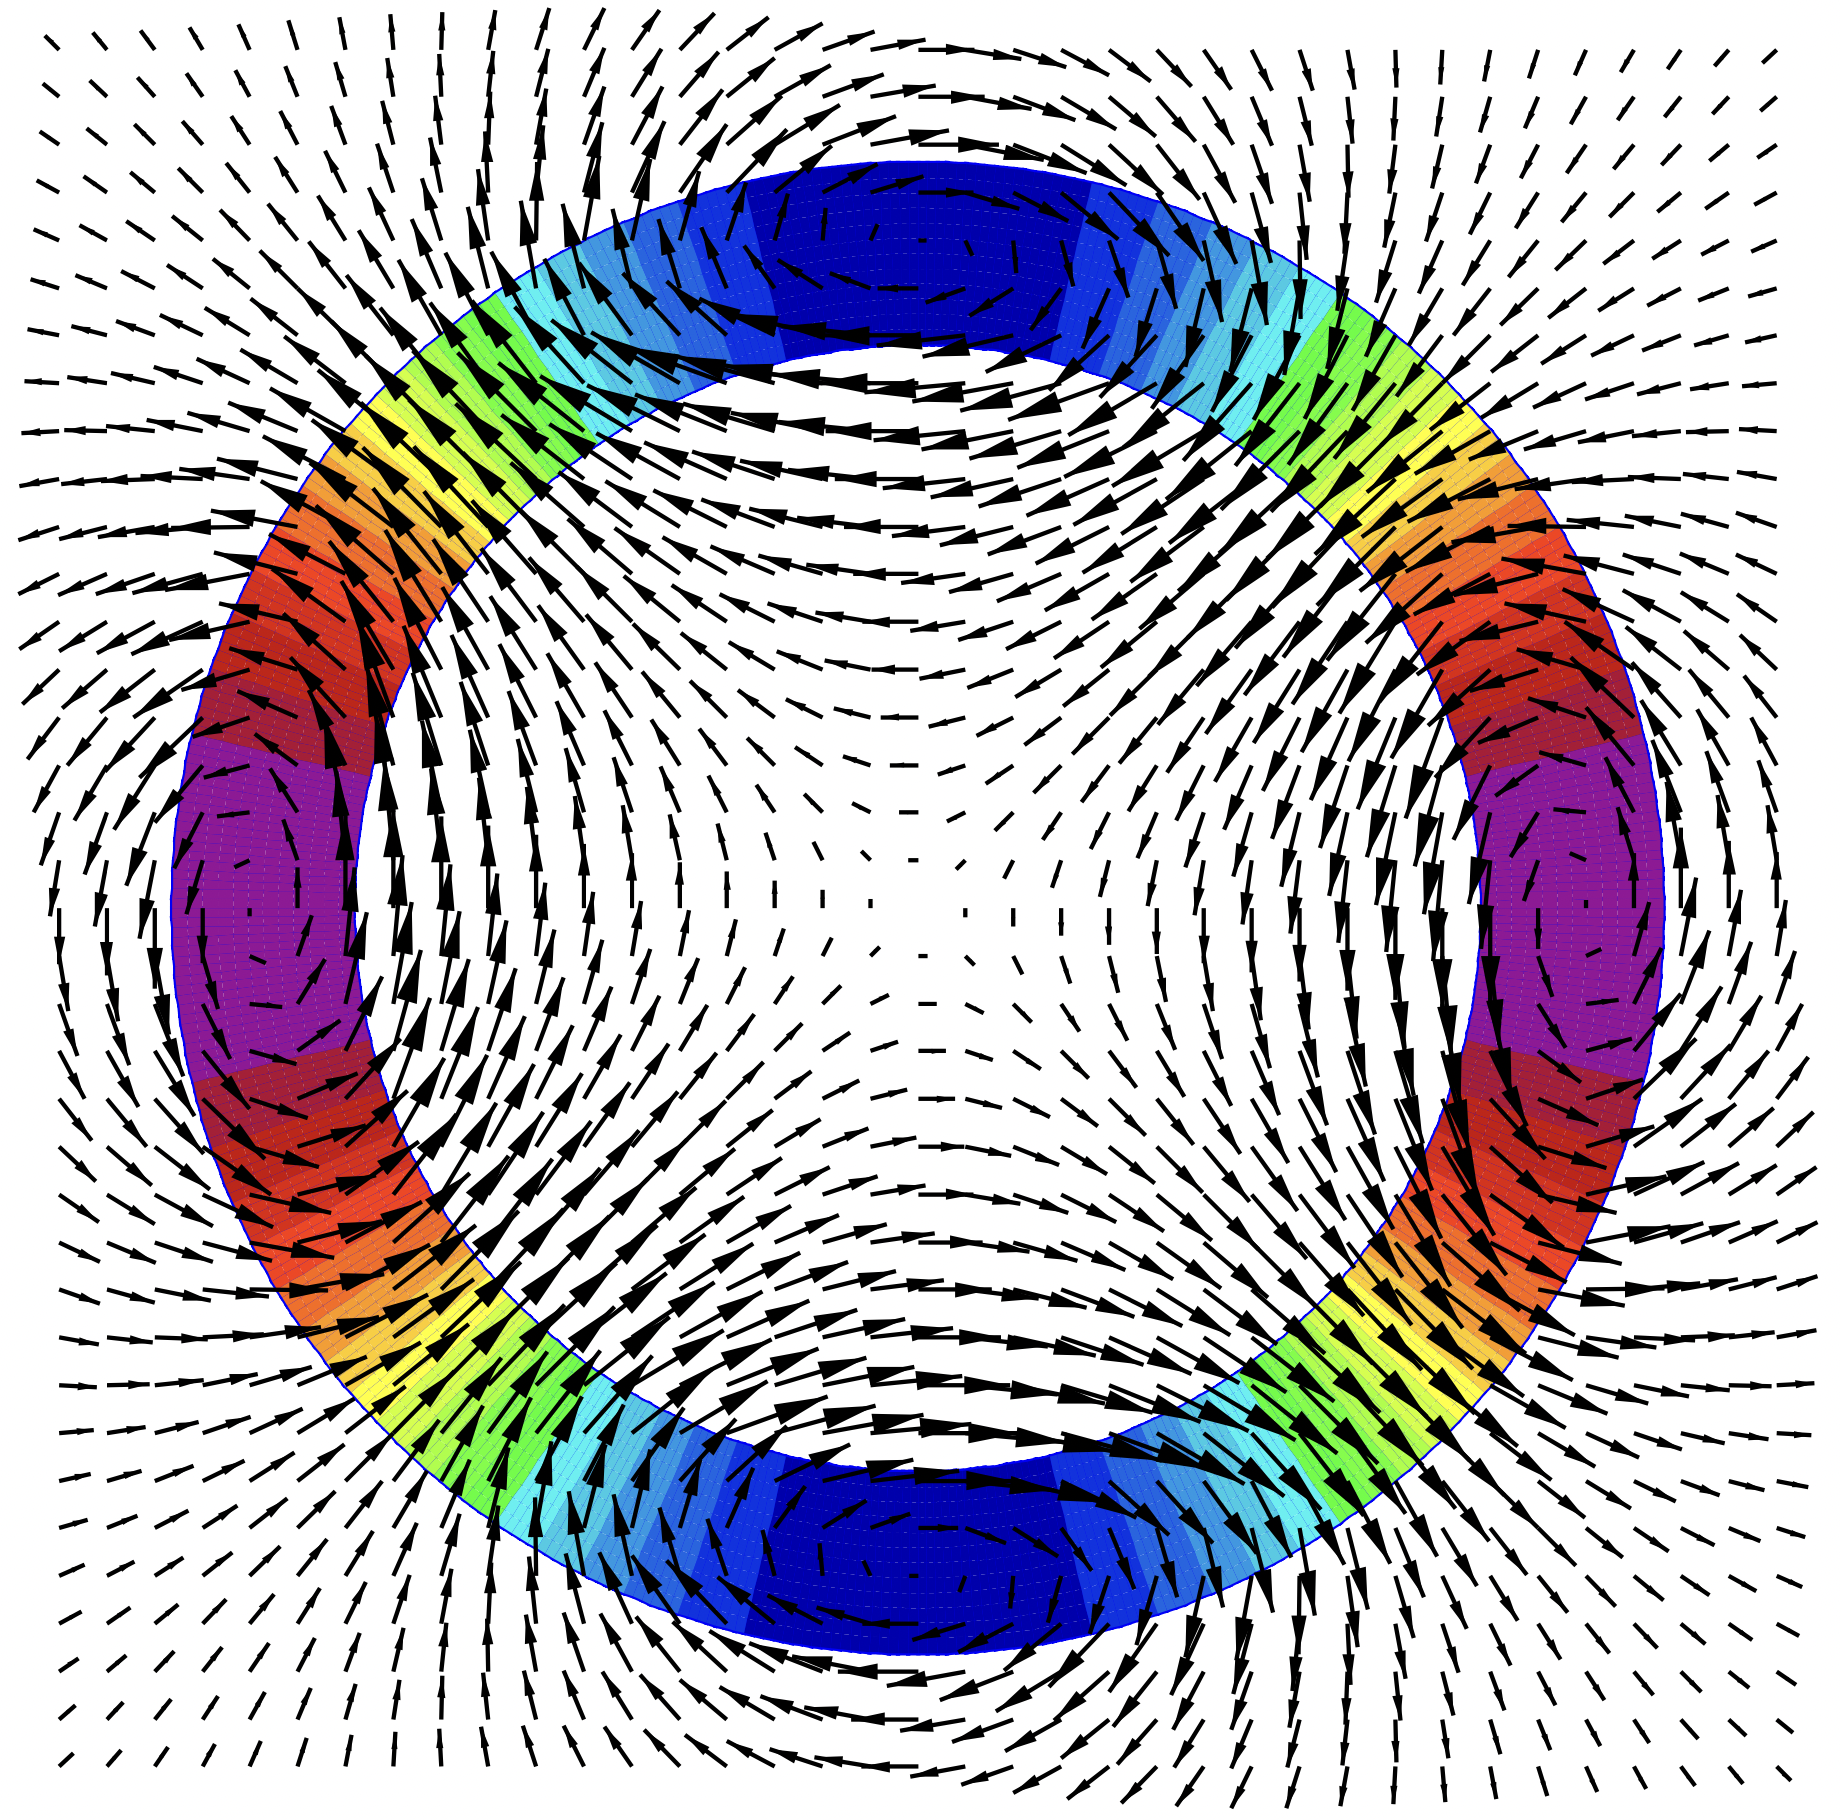
\includegraphics[width=6.5cm]{Figures/Beam_Dynamics_Theory/ideal_quadrupole_cos_2theta.png}
        \label{fig:ideal_quadrupole}
    }
    \caption{Magnetic fields and forces in an idealized dipole and quadrupole, with a \(\cos(\theta)\) and \(\cos(2\theta)\) current distribution in the circular coil, respectively. Current in the dipole and quadrupole coils are indicated in color. These visuals were taken from \cite{CERN:Russenschuck:CAS_Design_Magnets}.}
    \label{figure:dipole_quadrupole_fields}
\end{figure}

\subsection{Equations of Motion and Twiss Parameters}
\label{subsection:equations_of_motion_and_twiss_parameters}

The focusing from quadrupoles in a circular accelerator such as the LHC is periodic in \(s\), with a period of at most the circumference of the machine.
Assuming the existence of a closed orbit, the transverse motion of a single particle in a synchrotron with a periodic lattice is described by Hill's equation:

\begin{equation}
    u^{\prime \prime} + K_u(s) u(s) = 0; \quad u = x, y; \quad u^{\prime} = \dfrac{du}{ds} \text{ ,}
    \label{equation:hill_equation}
\end{equation}

where \(k\) describes the focusing forces action on the beam, and varies with \(s\) as it is dictated by magnetic elements traversed by particles.
A focusing quadrupole has a \(k > 0\), a focusing quadrupole has \(k < 0\), and a drift space has \(k = 0\).
The focusing strengths in the transverse planes go as:

\begin{equation}
	\begin{aligned}
		K_{x} &= \frac{1}{\rho^2} - k_{1} \text{ ,} \\
    	K_{y} &= k_{1} \text{ .}
	\end{aligned}
    \label{equation:transverse_focusing_strengths}
\end{equation}

The term \(\left(1 / \rho^2\right)\) in the horizontal component arises from the weak focusing caused by dipoles.
In the material below, \(u\) will be used to denote either \(x\) or \(y\), the rules applying to both similarly.
According to the theorem of Floquet~\cite{BOOK:Lee:Accelerator_physics}, the solution with periodic boundary conditions to Hill’s equation takes the form of \cref{equation:hill_solution}:

\begin{equation}
    \begin{aligned}
        u(s)          &= \sqrt{\beta_{u}(s) \varepsilon_{u}} \cos \left( \phi_{u}(s) + \phi_{u,0} \right) \text{ ,} \\
        u^{\prime}(s) &= -\sqrt{\frac{\varepsilon_u}{\beta_u(s)}} \left( \sin \left(\phi_u(s) + \phi_{u, 0} \right) + \alpha(s) \cos \left( \phi_u(s)+\phi_{u, 0} \right) \right) \text{ .}
    \end{aligned}
    \label{equation:hill_solution}
\end{equation}

These equations describe a harmonic oscillation in the transverse planes.
Here \(\varepsilon_u\) is the \intro{geometric emittance} of a particle and is a constant of the motion at a given energy. 
\(\phi_u(s)\) is the \intro{phase advance} and \(\alpha_u(s)\) is the \intro{alpha-function}.
\(\beta_u(s)\) is the \intro{beta-function} and represents the fluctuation of the oscillation envelope around the ring: it describes the transverse position dependent amplitude of the oscillation and has the dimension of a length.
In particle colliders such as the LHC the \betafunctions at the Interaction Points (IP), where the beams are made to collide, are commonly referred to as \(\beta_u^{\ast}\).
The solution of Hill's equation can also be written in matrix form as:

\begin{equation}
    \left(
        \begin{array}{c}
            u(s) \\
            u^{\prime}(s)
        \end{array} \right) = \mathrm{M} \left( 
        \begin{array}{c}
            u(0) \\
            u^{\prime}(0)
    \end{array} \right) \text{ .}
    \label{equation:hill_solution_matrix}
\end{equation}

In this form, which makes the assumption that the magnetic field of an element is constant along the longitudinal direction, M is called a \intro{transfer matrix}. 
Below are the transfer matrices corresponding to a drift space, \(\mathrm{M_{drift}}\), a dipole, \(\mathrm{M_{dip.}}\), a focusing quadrupole, \(\mathrm{M_{foc. quad.}}\), and a defocusing quadrupole \(\mathrm{M_{defoc. quad.}}\), respectively.

\begin{equation}
    \mathrm{M_{drift}} = \left(
        \begin{array}{ll}
            1 & L \\
            0 & 1
    \end{array} \right) \text{ ,}
    \label{equation:drift_transfer_matrix}
\end{equation}

\begin{equation}
    \mathrm{M_{dip.}} = \left(
        \begin{array}{cc}
            \cos \theta           & \rho \sin \theta \\
            - \sin \theta / \rho  & \cos \theta
    \end{array} \right) \text{ ,}
    \label{equation:dipole_transfer_matrix}
\end{equation}

\begin{equation}
    \mathrm{M_{foc. quad.}} = \left(
        \begin{array}{cc}
            \cos \left( \sqrt{k_1} L \right)             & \frac{1}{\sqrt{k_1}} \sin \left( \sqrt{k_1} L \right) \\
            -\sqrt{k_1} \sin \left( \sqrt{k_1} L \right) & \cos \left( \sqrt{k_1} L \right)
    \end{array} \right) \text{ ,}
    \label{equation:focusing_quad_transfer_matrix}
\end{equation}

\begin{equation}
    \mathrm{M_{defoc. quad.}} = \left(
        \begin{array}{cc}
            \cosh \left( \sqrt{\abs{k_1}} L \right)                 & \frac{1}{\sqrt{\abs{k_1}}} \sinh \left( \sqrt{\abs{k_1}} L \right) \\
            \sqrt{\abs{k_1}} \sinh \left( \sqrt{\abs{k_1}} L \right) & \cosh \left( \sqrt{\abs{k_1}} L \right)
    \end{array} \right) \text{ ,}
    \label{equation:defocusing_quad_transfer_matrix}
\end{equation}
where \(L\) is the element length and \(\theta = L / \rho\) is the bending angle of the dipole.
The transfer matrix of a group of elements is obtained by multiplying the transfer matrices of all individual elements.
For example, the transfer matrix corresponding to the \(\mathrm{FODO}\) cell of \cref{figure:fodo_cell_schematic} is:

\begin{equation}
    \mathrm{M_{FODO}} = \mathrm{M_{foc. quad.}} \mathrm{M_{drift}} \mathrm{M_{defoc. quad.}} \mathrm{M_{drift}} \text{ .}
    \label{equation:fodo_transfer_matrix}
\end{equation}

For a complete machine with hundreds to thousands of elements, the maps of linear elements can still be combined to obtain the coordinates of a particle after a full revolution.
This specific transfer map is called the \intro{one-turn map} and fully describes the linear evolution of a particle's coordinates over one revolution of the accelerator.
It can be expressed as

\begin{equation}
    \mathrm{M_{OTM}} = \mathrm{M_N} \cdot \mathrm{M_{N-1}} \cdot \ldots \cdot \mathrm{M_2} \cdot \mathrm{M_1} \text{ ,}
    \label{equation:one_turn_map}
\end{equation}
where \(\mathrm{M_i}\) is the transfer matrix of the \(i\)th element in the machine.
The transformation of coordinates over a revolution is then given by

\begin{equation}
    \left(
        \begin{array}{c}
            u \\
            u^{\prime}
        \end{array} \right)_{s_0 + C} = \mathrm{M_{OTM}} \cdot \left( 
        \begin{array}{c}
            u \\
            u^{\prime}
    \end{array} \right)_{s_0} \text{ .}
    \label{equation:one_turn_coordinates_transformation}
\end{equation}

The phase advance \(\phi_u(s)\) mentioned above corresponds to the difference of the betatron phase functions at two points, typically also taken with respect to an arbitrary initial point at \(s = 0\).
The phase advance between two points at longitudinal positions \(s_1\) and \(s_2\) in the lattice is defined as:

\begin{equation}
    \phi_{s_1 \rightarrow s_2} = \phi(s_{2}) - \phi(s_{1}) = \int_{s_{1}}^{s_{2}} \frac{1}{\beta(s)} ds \text{ .}
\end{equation}

As particles go around the ring, they oscillate around the closed orbit within an enveloppe defined by the \betafunctions and the emittance.
The number of these so-called \intro{betatron oscillations} per revolution is the \intro{tune} \(Q_u\).
The tune is defined in \cref{equation:tune_definition}, where \(\Delta \phi_{x, y}\) is the total betatron phase advance of a particle over a full circumference:

\begin{equation}
    Q_{u} = \frac{1}{2 \pi} \Delta \phi_{u} = \frac{1}{2 \pi} \oint_C \dfrac{ds}{\beta_{u} (s)} \text{ .}
    \label{equation:tune_definition}
\end{equation}

The \alphafunction is defined via the derivative of the \betafunction by:

\begin{equation}
    \alpha_u(s) = - \frac{1}{2} \beta^{\prime}_u(s) \text{ .}
    \label{equation:alpha_function}
\end{equation}

Similarly to the \(\beta\)-function, the \intro{gamma-function} \(\gamma_u(s)\) describes the envelope of oscillations in \(x^{\prime}\) and \(y^{\prime}\).
Both quantities are related by the \alphafunction according to:

\begin{equation}
    \gamma_u(s) = \frac{1 + \alpha_u^2(s)}{\beta_u(s)} \text{ .}
    \label{equation:gamma_function}
\end{equation}

The \(\alpha_u (s)\), \(\beta_u (s)\), \(\gamma_u (s)\) and \(\phi_u (s)\) are also called the \intro{Twiss parameters}.
The transfer matrix can be expressed with Twiss parameters according to~\cite{AOP:COURANT:Theory_Alternating_Gradient_Synchrotron}:

\begin{equation}
    \mathrm{M} = 
    \left( 
    \begin{array}{ll}
        m_{11} & m_{12} \\
        m_{21} & m_{22}
    \end{array} \right) 
    = 
    \left(
    \begin{array}{cc}
        \cos(\phi_u) + \alpha_u \sin(\phi_u) & \beta_u \sin(\phi_u) \\
        - \gamma_u \sin(\phi_u)              & \cos(\phi_u) - \alpha_u \sin(\phi_u)
    \end{array} 
    \right) \text{ .}
    \label{equation:transfer_matrix_twiss_parameters}
\end{equation}

\subsection{Phase Space Ellipse}
\label{subsection:phase_space_ellipse}

In the linear regime all particle trajectories describe ellipses in \((u, u^{\prime})\) phase space.
The geometric emittance \(\varepsilon_u\) introduced in \cref{equation:hill_solution}, also named the \intro{Courant-Snyder invariant}, defines together with the Twiss parameters \(\alpha_u (s)\), \(\beta_u (s)\) and \(\gamma_u (s)\) the equation of the phase space ellispe:

\begin{equation}
    \gamma_{u}(s) u^{2} + 2 \alpha_{u}(s) u(s) u^{\prime}(s) + \beta_{u}(s) u^{\prime}(s)^{2} = \varepsilon_u \text{ .}
    \label{equation:ellipse_equation}
\end{equation}

\Cref{figure:phase_space_ellipse} shows a schematic illustration of the phase space ellipse, the area of which is defined by the geometric emittance according to:

\begin{equation}
    A = \pi \varepsilon_u \text{ .}
    \label{equation:phase_space_ellipse_area}
\end{equation}

\begin{figure}[!htb]
    \begin{center}
    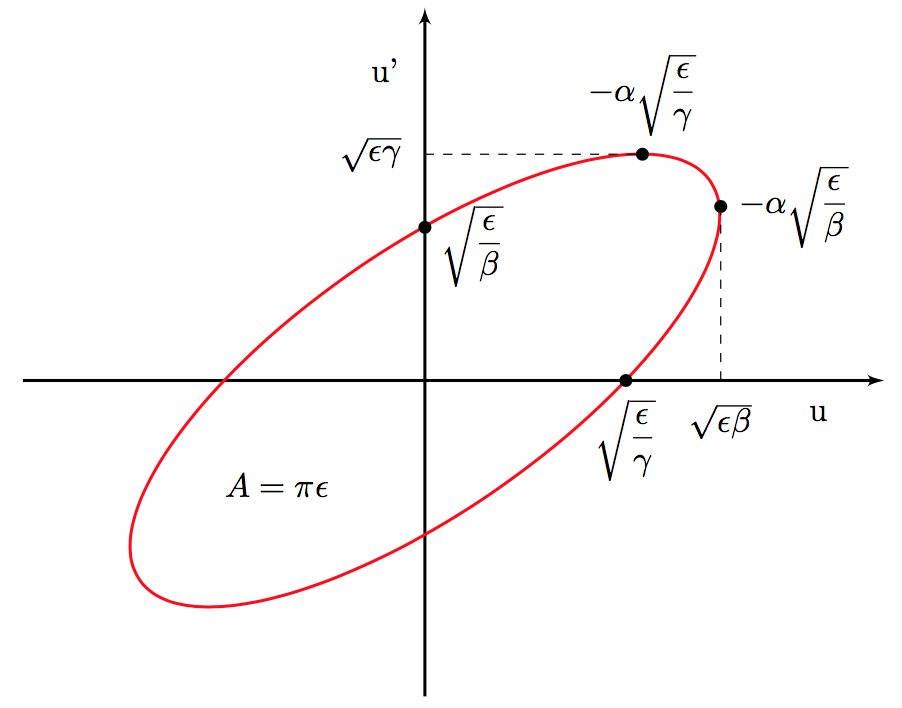
\includegraphics[width = 0.75\linewidth]{Figures/Beam_Dynamics_Theory/Phase_Space.png}
    \caption{Phase space ellipse in the transverse \((u, u^{\prime})\) plane, where \(u\) represents either transverse coordinate \(x\) or \(y\).}
    \label{figure:phase_space_ellipse}
    \end{center}
\end{figure}

According to the Liouville theorem, the phase space volume, the ellipse area \(A\) is a constant in a closed system.
When accelerating the beam this theorem no longer holds true and the geometric emittance \(\varepsilon\) will decrease as the beam energy increases.
One can then construct the \intro{normalized emittance} \(\varepsilon_{\gamma}\), which is invariant with beam energy, based on the relativistic beta and gamma:

\begin{equation}
    \varepsilon_u^{\mathrm{norm}} = \beta_{\mathrm{rel}} \gamma_{\mathrm{rel}} \varepsilon_u \text{ .}
    \label{equation:normalized_emittance}
\end{equation}

When referring to the emittance of a specific particle one uses the term \intro{single particle emittance}.
The \intro{action} \(J_u\) is related to the single particle emittance by:

\begin{equation}
    2 J_u = \varepsilon_u \text{ .}
    \label{equation:single_particle_action}
\end{equation}

The state of particles in phase space can be fully characterized by the action variable and the corresponding phase variable seen above. 

Different particles in the beam will have different single particle emittances and will undergo betatron oscillations of varying amplitudes.
For a Gaussian shaped beam the transverse beam size is defined as:

\begin{equation}
    \sigma_u = \sqrt{\beta_u(s) \varepsilon_u^{\mathrm{beam}}} \text{ ,}
    \label{equation:gaussian_beam_transverse_beam_size}
\end{equation}
with \(\varepsilon_u^{\mathrm{beam}}\) the beam emittance, typically defined the emittance corresponding to a \(1 \sigma\) amplitude of the Gaussian charge distribution.
In the case of more general particle distributions an alternative definition of the beam emittance is often used~\cite{CERN:Muller:Beam_Matter_Covariance_Matrix_Emittance, CERN:Buon:CAS_Beam_Phase_Space_Emittance}:

\begin{equation}
    \varepsilon_u^{\mathrm{rms}} = \sqrt{\left\langle u \right\rangle^{2} \left\langle u^{\prime} \right\rangle^{2} - \left\langle uu^{\prime} \right\rangle^{2}} \text{ .}
    \label{equation:beam_emittance_general}
\end{equation}

The phase space trajectory of a particle depends on the Twiss parameters \(\alpha(s)\), \(\beta(s)\), and \(\gamma(s)\).
One can remove this dependency by performing a coordinate transformation to the \intro{Courant-Snyder coordinates}~\cite{BOOK:Bazzani:Normal_Form_Approach_Betatron_Motion}, defined as:

\begin{equation}
    \left(\begin{array}{c}
    \hat{u} \\
    \hat{u}^{\prime}
    \end{array}\right) = \left(\begin{array}{cc}
    \frac{1}{\sqrt{\beta_{u}(s)}} & \frac{\alpha_{u}(s)}{\sqrt{\beta_{u}(s)}} \\
    0 & \sqrt{\beta_{u}(s)}
    \end{array}\right)\left(\begin{array}{c}
    u \\
    u^{\prime}
    \end{array}\right) \text{ ,}
    \label{equation:physical_to_courant_snyder_coordinates}
\end{equation}
where the Courant-Snyder coordinates are denoted by \^{}.
In this new system particles follow circular trajectories in phase space.
\Cref{figure:physical_to_normalized_courant_snyder_coordinates} provides an illustrative representation of phase space in both physical and normalized coordinates for an accelerator with linear elements only.
In the new representation, the elliptical phase space is transformed into a simpler circular phase space where the motion is described by simple rotations, fully described by and dependeing only on the action and angle variables \((J_u, Q_u)\).

\begin{figure}[!htb]
    \begin{center}
    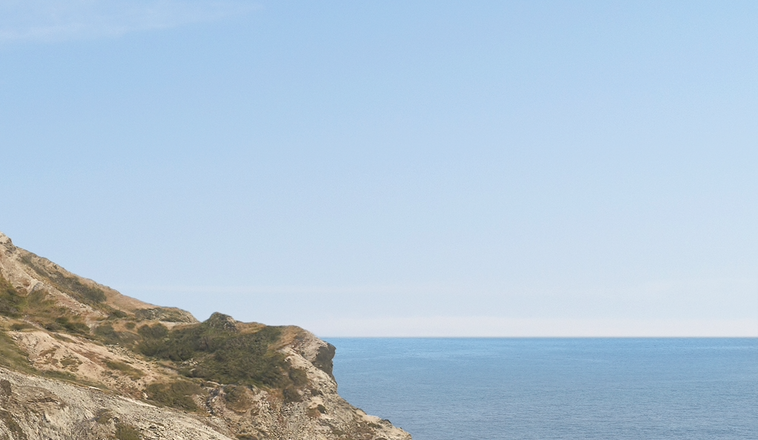
\includegraphics[width = 0.75\linewidth]{Figures/placeholder.png}
    \caption{\todo{Figure 2.6 from F. Carlier PhD?}}
    \label{figure:physical_to_normalized_courant_snyder_coordinates}
    \end{center}
\end{figure}

\subsection{Chromatic Effects}
\label{subsection:chromatic_effects}

Until now, it was assumed that all particles had the intended design momentum \(p_{0}\).
Naturally, in practice particles withing the beam have a distribution in energy and momentum.
For a particle with a momentum \(p \neq p_{0}\) one defines and uses the \textit{relative momentum deviation} \(\delta\): the deviation from the reference orbit from the momentum deviation.

\begin{equation}
    \delta = \frac{p - p_{0}}{p_{0}} = \frac{\Delta p}{p} \text{ .}
    \label{equation:momentum_deviation}
\end{equation}

Such momenta offsets introduce \intro{chromatic errors} in the beam dynamics.
Effects and parameters depending on \(\delta_p\) are called \intro{chromatic effects}.

From the definition of the magnetic rigidity in \cref{equation:magnetic_rigidity}, it follows that particles of different momenta will have different local radii of curvature when going through dipoles and therefore follow different orbits along the machine.
The deviation of an off momentum particle orbit from that of the synchronous particle is defined by the \intro{dispersion function} \(D(s)\).
Its contribution to a particle's orbit in a region of non-zero dispersion is described by:

\begin{equation}
    \Delta u_{\mathrm{dispersion}} = D_{u}(s) \delta \text{ .}
    \label{equation:dispersion_contribution_to_orbit}
\end{equation}
\bigbreak

Off-momentum particle positions scale linearly with dispersion, and in its presence \cref{equation:hill_solution} is extended to~\cite{BOOK:Wiedemann:Particle_Accelerator_Physics}:

\begin{equation}
    u(s) = \sqrt{\varepsilon_u \beta_u(s)} \cos \left( \phi_u(s) + \phi_{u, 0} \right) + D_u(s) \delta_p \text{ .}
    \label{equation:hill_solution_with_dispersion}
\end{equation}

Another chromatic parameter is the \intro{chromaticity} \(Q_u^{\prime}\), which describes the tune shift \(\Delta Q_u\) with particle momentum by

\begin{eqnarray}
    Q^{\prime}_u = \frac{\Delta Q_u}{\delta_p} \text{ .}
    \label{equation:chromaticity_definition}
\end{eqnarray}

The effective focusing strength of quadrupoles, which is inversely proportional to the momentum, differs for off momentum particles.
The change of focusing strength due to energy deviation is:

\begin{equation}
	\Delta k_{1} = - \dfrac{e}{p^2} \dfrac{d B_{y}}{d x} \Delta p = -k_{1} \delta_p \text{ .}
    \label{equation:quadrupole_focusing_strength_deviation_from_dispersion}
\end{equation}

This quadrupole error results in a tune shift proportional to the energy offset:

\begin{equation}
	\Delta Q = \dfrac{1}{4 \pi} \int \beta(s) \Delta k_{1}(s) ds = \left[ - \frac{1}{4 \pi} \int \beta(s) k_{1}(s) ds \right] \delta \text{ .}
    \label{equation:tune_shift_from_dispersion}
\end{equation}

The natural chromaticity of a linear lattice can then be approximated by~\cite{CAS:Guiducci:Chromaticity}:

\begin{equation}
    Q_u^{\prime} \approx -\frac{1}{4 \pi} \oint \beta_u(s) K_u \mathrm{d}s \text{ .}
    \label{equation:natural_chromaticity_approximation}
\end{equation}

%----------------------------------------------------------------------------------------

\section{Non-Linear Magnetic Multipoles}
\label{section:non_linear_magnetic_multipoles}

Magnetic fields of sextupolar and higher order are called \intro{non-linear} magnetic fields.
While only dipolar and quadrupolar magnetic fields are considered in the linear approximation, non-linear magnetic fields are present in most accelerators.
They can be introduced by design or by the presence of flaws in lower order magnets, the latter having the potential to seriously disrupt the beam.

The order of a multipole is labeled \(n\), with the convention that \(n = 1\) corresponds to a magnetic dipole, \(n = 2\) to a quadrupole, \(n = 3\) a sextupole etc.
The magnetic field of a multipole of order \(n\) is given by:

\begin{equation}
    \begin{aligned}
    B_y(x, y, s) + i B_x(x, y, s) & = \sum_{n=1}^{\infty} \left[ B_n(s) + i A_n(s) \right] (x + i y)^{n-1} \text{ ,} \\
    B_n(s)                        & = \left. \frac{1}{(n - 1) !} \frac{\partial^{n - 1} B_y}{\partial x^{n - 1}} \right|_{(0,0,s)} \text{ ,} \\
    A_n(s)                        & = \left. \frac{1}{(n - 1) !} \frac{\partial^{n - 1} B_x}{\partial x^{n - 1}} \right|_{(0,0,s)} \text{ .} 
    \end{aligned}
    \label{equation:multipole_expansion}
\end{equation}

Here \(B_n(s)\) and \(A_n(s)\) are the normal and skew multipole coefficients, respectively, where a skew magnet is rotated by \(\pi / (2 n)\) with respect to its normal counterpart.
In the linear regime, the Hamiltonian may be written as

\begin{equation}
    \mathcal{H} = \frac{1}{2} p_x^2 + \frac{1}{2} p_y^2 + \frac{1}{2} K(s) x^2 - \frac{1}{2} K(s) y^2 \text{ ,}
    \label{equation:hamiltonian_linear_lattice}
\end{equation}
where \(K(s)\) describes the variation of focusing strength around the ring.

Starting from the Hamiltonian equations

\begin{equation}
    \dfrac{d \vec{p_z}}{d t} = - \frac{\partial \mathcal{H}}{\partial \vec{z}} \text{ ,} \quad \quad \quad \dfrac{d \vec{z}}{d t} = \frac{\partial \mathcal{H}}{\partial \vec{p_z}} \text{ ,}
    \label{equation:hamiltonian_equations}
\end{equation}
the Hamiltonian for the transverse planes for a multipole of order n is given by \cref{equation:hamiltonian_multipole_order_n}~\cite{PHD:Tomas, PHD:Franchi}:

\begin{equation}
    \mathcal{H} = \frac{q}{p} \operatorname{Re} \left[ \left( B_n +i A_n \right) \frac{(x + i y)^n}{n} \right] \text{ .}
    \label{equation:hamiltonian_multipole_order_n}
\end{equation}

If the Hamiltonian for a normal multipole of order \(n\) is labeled \(N_n\), and the Hamiltonian for a skew multipole of order \(n\) is labeled \(S_n\), then~\cite{PHD:Maclean, PHD:Persson}:

\begin{equation}
    \begin{aligned}
        N_n & \propto \operatorname{Re} \left[(x + i y)^n \right] \\
            & \propto \operatorname{Re} \left[ \sum_{k=0}^n \left(
                \begin{array}{l}
                    n \\
                    k
                \end{array} \right) 
            i^k \beta_x^{\frac{n-k}{2}} \beta_y^{\frac{k}{2}} \left(\sqrt{2 J_x} \cos \phi_x \right)^{n-k} \left( \sqrt{2 J_y} \cos \phi_y \right)^k \right] \text{ ,}
    \end{aligned}
    \label{equation:hamiltonian_prop_normal_multipoles}
\end{equation}

\begin{equation}
    \begin{aligned}
        S_n & \propto \operatorname{Im} \left[(x + i y)^n \right] \\
            & \propto \operatorname{Im} \left[ \sum_{k=0}^n \left(
                \begin{array}{l}
                    n \\
                    k
                \end{array} \right) 
            i^k \beta_x^{\frac{n-k}{2}} \beta_y^{\frac{k}{2}} \left(\sqrt{2 J_x} \cos \phi_x \right)^{n-k} \left( \sqrt{2 J_y} \cos \phi_y \right)^k \right] \text{ .}
    \end{aligned}
    \label{equation:hamiltonian_prop_skew_multipoles}
\end{equation}

The powering of non-linear magnets and the presence of magnetic errors can have a significant impact on the beam dynamics.
Geometric errors can contribute to the presence of non-linear components too.
For instance, when a particle does not pass through the magnetic center of an element it will see not only the primary field component but also perturbations of all lower orders to that of the traversed element~\cite{BOOK:Wiedemann:Particle_Accelerator_Physics}.

This effect is called \intro{feed-down} and can be introduced by misalignment of lattice elements, which would cause the closed orbit to deviate from the ideal one and the beam to pass off-axis in magnets.
Should that happen with a sextupole, for instance, the beam would experience a sextupolar field but also encounter quadrupolar and dipolar components.

The rotational misalignment of elements is also a concern, as rotation a purely normal or skew multipole results in the beam experiencing a combination of both normal and skew fields.

%----------------------------------------------------------------------------------------

\section{Non-Linear Formalism and Resonance Driving Terms}
\label{section:non_linear_formalism_and_rdts}

The material below is inspired from~\cite{PHD:Tomas, PHD:Franchi,PHD:Maclean, PHD:Persson} where some aspects of it may be found in more details.
For the curious reader, a very thourough approach to normal forms can be found in~\cite{PRAB:Franchi:First_Simultaneous, PHD:Carlier}.

\subsection{Non-Linear Transfer Maps}
\label{subsection:non_linear_transfer_maps}

As introduced in \cref{equation:one_turn_map}, the dynamics of a circular accelerator can be parametrized in terms of \intro{transfer maps} relating final to initial phase space coordinates.
This approach is described in~\cite{BOOK:Bazzani:Normal_Form_Approach_Betatron_Motion, JMP:Forest:Hamiltonian_Free_Description_Single_Particle_Dynamics}.
While the transfer map of a linear element is described by a matrix, that of a non-linear element is itself described by the exponential \intro{Lie operator} \(e^{-:f:}\) defined as~\cite{BOOK:Wolski:Beam_dynamics}:

\begin{equation}
    \begin{aligned}
        e^{-:f:} g          &= g + \left[f, g\right] + \frac{1}{2} \left[f, \left[f, g \right] \right] + \ldots \text{ ,} \\
        \left[ f, g \right] &= \sum_i \frac{\partial f}{\partial q_i} \frac{\partial g}{\partial p_i} - \frac{\partial f}{\partial p_i} \frac{\partial g}{\partial q_i} \text{ ,}
    \end{aligned}
    \label{equation:lie_operator}
\end{equation}
where \(q_i\) and \(p_i\) are the canonical coordinates and momenta, respectively.
Here \(\left[ f, g \right]\) is the \intro{Poisson bracket} of \(f\) and \(g\).
When including non-linear sources, the one-turn map introduced in \cref{equation:one_turn_map} becomes:

\begin{equation}
    \mathcal{M } =e^{-:h_N:} e^{-:h_{N-1}:} \ldots e^{-:h_2:} e^{-:h_1:} R \text{ ,}
    \label{equation:one_turn_map_non_linear}
\end{equation}
where \(R\) is a matrix describing the linear dynamics of the machine, and the \(h_i\) terms represent the thin kick Hamiltonians of the non-linear elements in the accelerator.
\break

Relevant properties of the exponential Lie operator can be found in~\cite{PHD:Tomas, PHD:Franchi}, one of which being that the product of exponential Lie operators can be expressed as another exponential Lie operator following the \emph{Campbell-Baker-Hausdorff} theorem.
The one-turn map becomes:

\begin{equation}
    \mathcal{M} = e^{-:h:} R \text{ ,}
    \label{equation:Campbell_Baker_Hausdorff_theorem}
\end{equation}
in which, in case the \(h_n\) are small, \(h\) can be approximated as:
\begin{equation}
    h = \sum_{n=1}^N h_n + \sum_{n, m<n}^N \left[ h_m, h_n \right] + \ldots \text{ .}
    \label{equation:h_thin_kick_approximation}
\end{equation}

Using only the first order in \(h_n\), the thin kick \(h\) can be expressed in expanded terms using the action and angle variables according to:

\begin{equation}
    h = \sum_{jklm} h_{jklm} \left( 2 J_x \right)^{\frac{j+k}{2}} \left( 2 J_y \right)^{\frac{l+m}{2}} e^{i \left[ \left(j-k\right) \left(\phi_x - \phi_{x,0} \right) + \left(l-m\right) \left(\phi_y - \phi_{y,0} \right) \right]} \text{ ,}
    \label{equation:h_thin_kick_expansion}
\end{equation}
with \(h_{jklm}\) being the \intro{Hamiltonian coefficient} encompassing the contribution of all multipoles of order \(n = j + k + l + m\). 
The derivation for the result of \cref{equation:h_thin_kick_expansion} can be found in \cref{appendix:hamiltonian_derivation}.

A multipole of order \(n = j + k + l + m\) gives rise to terms in the Hamiltonian \(\propto x^{j+k} y^{l+m}\).
In the case of a skew quadrupole (\(n=2\)) for example, one will see terms in the Hamiltonian \(\propto xy\), meaning a contribution to \(h_{1010}\), \(h_{1001}\), \(h_{0110}\) and \(h_{0101}\).

\subsection{Normal Form, Resonance Driving Terms and Resonances}
\label{subsection:normal_form_and_rdt}

Due to the presence of non-linear sources the linear invariant \(J_u\) introduced in \cref{subsection:phase_space_ellipse} is no longer a constant.
This leads to the phase space trajectory in normalized, or Courant-Snyder, coordinates no longer describing a circle.
One may wish to create a new transformation, akin to that to normalized coordinates, that would allow describing betatron motion in phase space by a pure rotation in the presence of non-linear sources.

The change of coordinates is represented by a similarity transformation of the one turn map, written as~\cite{PHD:Tomas}:

\begin{equation}
    e^{-:F:} e^{:h:} R e^{:F:} \text{ ,}
    \label{equation:normal_form_transformation}
\end{equation}
where \(F\) is the \intro{generating function} of the transformation.
The coordinates resulting from the transformation are called \intro{normal form coordinates}.
This is illustrated in \cref{figure:physical_to_normalized_courant_snyder_coordinates}.

\begin{figure}[!htb]
    \begin{center}
    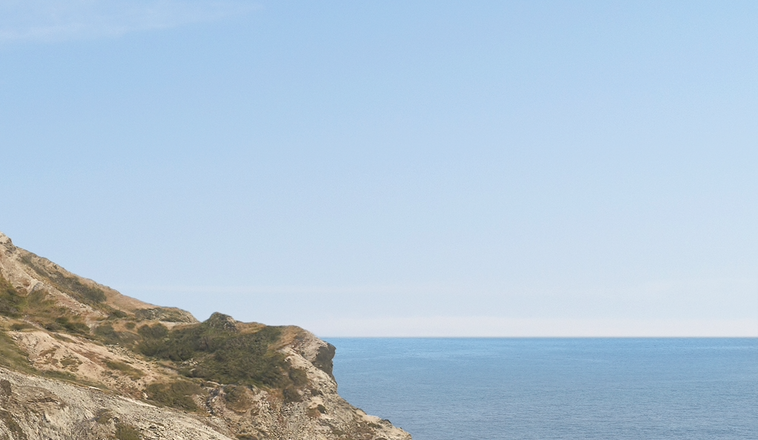
\includegraphics[width = 0.5\linewidth]{Figures/placeholder.png}
    \caption{\todo{Transformation to normal form coordinates (Ewen fig 1.5, Roro fig 3.1, or Felix fig 2.11)}}
    \label{figure:phase_space_physical_normalized_normal_form_coordinates}
    \end{center}
\end{figure}

The generating function of the transformation \(F\) contains a large portion of the information describing the non-linear dynamics, and a new non-linear invariant \(I_u\) can be introduced. 
Similarly to \(h\) in \cref{equation:h_thin_kick_expansion}, the generating function \(F\) can be expanded in terms of the normal form coordinates according to \todo{REF}:

\begin{equation}
    F = \sum_{jklm} f_{jklm} \left( 2 I_x \right)^{\frac{j+k}{2}} \left(2 I_y \right)^{\frac{l+m}{2}} e^{i \left[ (j-k) \left( \psi_x - \psi_{x_0} \right) + (l-m) \left( \psi_y - \psi_{y_0} \right) \right]} \text{ ,}
    \label{equation:generating_function_expansion}
\end{equation}
where \((I_u, \psi_u)\) are to normal form coordinates what \((J_u, \phi_u)\) are to normalized coordinates.
The \(f_{jklm}\) coefficients are related to the \(h_{jklm}\) terms by:

\begin{equation}
    f_{jklm} = \frac{h_{jklm}}{1 - e^{i 2 \pi \left[ \left(j-k\right) Q_x + \left(l-m\right) Q_y \right]}} \text{ .}
    \label{equation:resonance_driving_terms}
\end{equation}

From \cref{equation:resonance_driving_terms} one can see that the \(f_{jklm}\) coefficients diverge for certain values of the tunes.
Specifically, divergence happens when the following relation is satisfied:

\begin{equation}
    \left(j-k\right) Q_x + \left(l-m\right) Q_y = p \quad \quad \text { where } j, k, l, m, p \in \mathcal{Z} \text{ .}
    \label{equation:resonance_condition}
\end{equation}

A divergence of the \(f_{jklm}\) terms leads to a divergence of the transformation to normal form coordinates, which generally indicates an unclosed phase space trajectory due to a resonance in the beam motion.
The condition in \cref{equation:resonance_condition} corresponds to situations where particles lie on resonant frequencies, typically causing their amplitudes to group unbounded by the dynamics.
Therefore the \(f_{jklm}\) terms are called \intro{resonance driving terms} (RDTs).

For this reason, the tune is one of the single most important design parameters in synchrotrons.
The chosen operational transverse tunes of a synchrotron are known to as its \intro{working point}, and should be chosen carefully in order to avoid resonances.
Resonances up to order \(n = 5\) are shown in \cref{figure:tune_diagram_fifth_order}, with lines of different orders differentiated from one another.

\begin{figure}[!htb]
    \begin{center}
    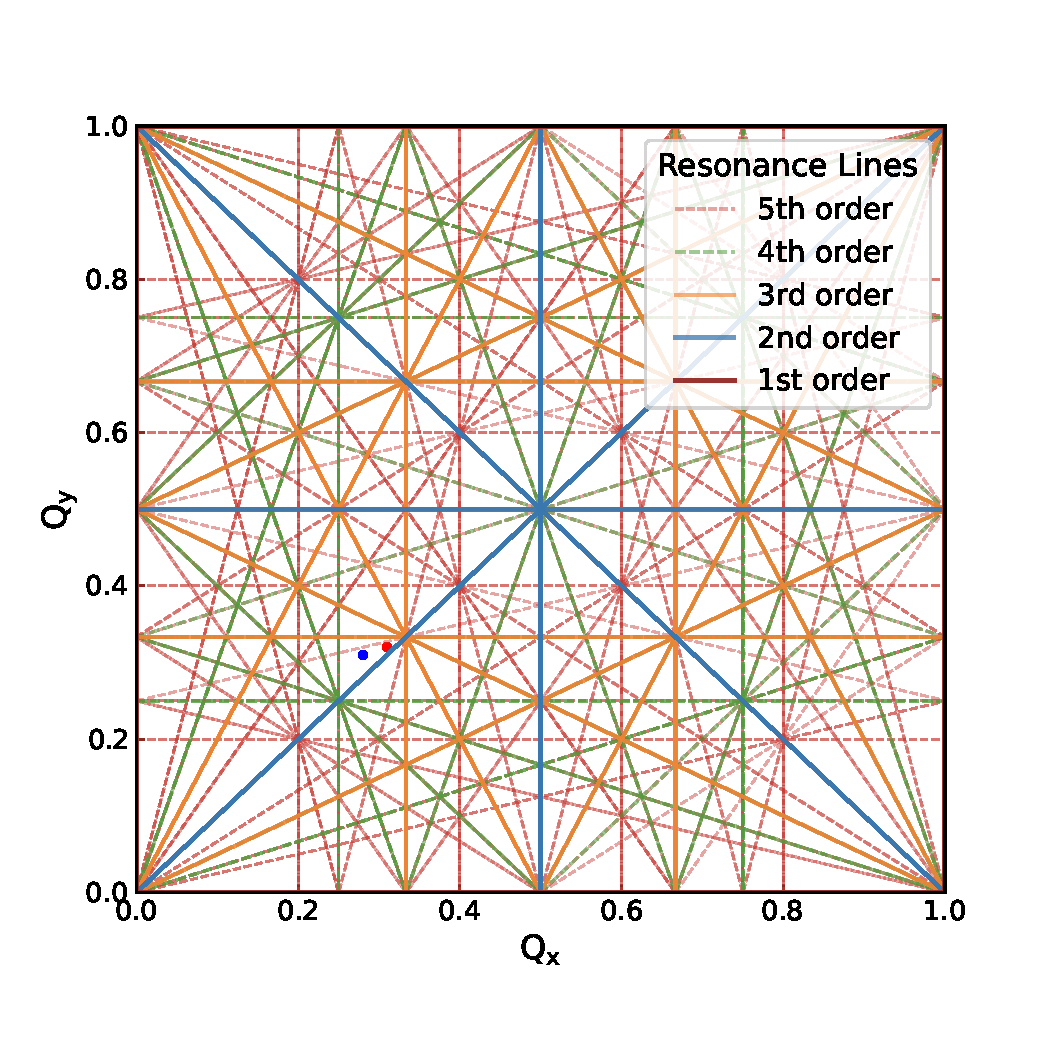
\includegraphics[width = 0.9\linewidth]{Figures/Beam_Dynamics_Theory/tune_diagram_fifth_order_with_working_points.pdf}
    \caption{Tunes diagram showing resonance lines up to order \(n = 5\). The LHC working points are indicated by the two dots: in \textcolor{wpblue}{blue} for injection tunes and \textcolor{wpred}{red} for collision tunes.}
    \label{figure:tune_diagram_fifth_order}
    \end{center}
\end{figure}

Commonly, the label of a given resonance is \(\left( n_1, n_2 \right)\), where \(n_1 = \left( j - k \right)\) and \(n_2 = \left( l - m \right)\).
Every generating function term \(f_{jklm}\), and equivalently every Hamiltonian term \(h_{jklm}\), is associated with a resonance.

The resonance driving terms vary in amplitude through the machine as they depend on local multipole strength of contributing sources.
Characteristically, the \(f_{jklm}\) terms show abrupt jumps at the location of relevant sources.

\todo{Maybe a figure of RDTs accross a known machine to illustrate?}

\subsection{Resonance Basis and Normal Form Coordinates}

The normalized Courant-Snyder coordinates \(\left( \hat{u}, \hat{p}_u \right)\) are related to the action and angle variables \(\left( J_u, \phi_u \right)\) by:

\begin{equation}
    \begin{aligned}
        \hat{u}   &= \sqrt{2 J_u} \cos \left( \phi_z - \phi_{z_0} \right) \text{ ,} \\
        \hat{p_u} &= - \sqrt{2 J_u} \sin \left( \phi_z - \phi_{z_0} \right) \text{ .}
    \end{aligned}
    \label{equation:normalized_courant_snyder_coordinates_from_action_angle}
\end{equation}

One can define the \intro{resonance basis} \(\left( h_x^{+}, h_x^{-}, h_y^{+}, h_y^{-} \right)\) by the relation:

\begin{equation}
    h_u^{\pm} = \hat{u} \pm i \hat{p}_z = \sqrt{2 J_u} e^{\mp i \left( \phi_u + \phi_{u_0} \right)} \text{ .}
    \label{equation:resonance_basis_definition}
\end{equation}

The transformation to the \kl{normal form coordinates} \(\left( \zeta_x^{+}, \zeta_x^{-}, \zeta_y^{+}, \zeta_y^{-} \right)\) is expressed as:

\begin{equation}
    \zeta_u^{\pm} = \sqrt{2 I_u} e^{\mp i \left( \psi_u + \psi_{u_0} \right)} = e^{-:F:} h_u^{\pm} \text{ .}
    \label{equation:transformation_to_normal_form_coordinates_from_h_pm}
\end{equation}
where \((I_u, \psi_u)\) are the terms introduced in \cref{equation:generating_function_expansion}.

By construction of the transformation, the one-turn map in normal form coordinates is an amplitude dependent rotation.
It follows that the motion of these coordinates as a function of the turn number is then given by:

\begin{equation}
    \zeta_u^{\pm}(N) = \sqrt{2 I_u} e^{\mp i \left( 2 \pi \nu_u N + \psi_{u_0} \right)} \text{ ,}
    \label{equation:normal_form_N_turn_expression}
\end{equation}
with \(\nu_u\) the transverse tunes.
The inverse transformation from the new action and angle variables to the Courant-Snyder variables is written, to first order, as:

\begin{equation}
    h_u^{-} = e^{:F:} \zeta_u^{-} \simeq \zeta_u^{-} + \left[ F, \zeta_u^{-} \right] \text{ .}
    \label{equation:inverse_transformation_normal_form-to_courant_snyder_coordinates}
\end{equation}

Using \cref{equation:normal_form_N_turn_expression} and \cref{equation:inverse_transformation_normal_form-to_courant_snyder_coordinates}, the linearly normalized coordinates can be expressed after \(N\) turns as:

\begin{equation}
    \begin{aligned}
        h_x^{-}(N) & = \sqrt{2 I_x} e^{i \left( 2 \pi \nu_x N - \psi_{x_0} \right)} \quad - \\
        & \quad 2 i \sum_{jklm} j f_{jklm} \left( 2 I_x \right)^{\frac{j+k-1}{2}} \left( 2 I_y \right)^{\frac{l+m}{2}}   e^{i \left[ (1-j+k) \left( 2 \pi \nu_x N-\psi_{x_0} \right) + (m-l)   \left( 2 \pi \nu_y N - \psi_{y_0} \right) \right]} \\
        h_y^{-}(N) & = \sqrt{2 I_y} e^{i \left( 2 \pi \nu_y N - \psi_{y_0} \right)} \quad - \\
        & \quad 2 i \sum_{jklm} l f_{jklm} \left( 2 I_x \right)^{\frac{j+k}{2}}   \left( 2 I_y \right)^{\frac{l+m-1}{2}} e^{i \left[ (k-j)   \left( 2 \pi \nu_x N-\psi_{x_0} \right) + (1-l+m) \left( 2 \pi \nu_y N - \psi_{y_0} \right) \right]} \text{ .}
    \end{aligned}
    \label{equation:linearly_normalized_coordinates_after_N_turns}
\end{equation}


\Cref{figure:coordinate_transformations} shows a schematic of the different transformations and changes to the one-turn map.
While one can calculate the evolution of the Courant-Snyder coordinates by applying the map \( \mathcal{M} \), the approach is complicated to solve.
Solving the one-turn map for the next turn is best done by performing a transformation to normal form coordinates \(\zeta_{u}^{\pm}\) using the generating function \(F\), applying the amplitude dependent rotation map \(R\), and transforming back to Courant-Snyder coordinates.
These calculations are in practice simpler than the former method, and conserve non-linearities.

\begin{figure}[!htb]
    \centering
    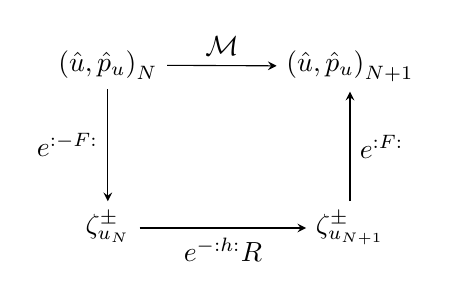
\begin{tikzpicture}
        \matrix (m) [matrix of math nodes,row sep=4em,column sep=4em,minimum width=2em]{
            \left(\hat{u}, \hat{p}_u\right)_N    &    \left(\hat{u}, \hat{p}_u\right)_{N+1} \\
            \zeta_{u_N}^{\pm}{}                  &    \zeta_{u_{N+1}}^{\pm}{}  \\
        };
        \path[-stealth]
        (m-1-1) edge node [above] {\( \mathcal{M} \)} (m-1-2)
        (m-1-1) edge node [left] {\( e^{:-F:} \)} (m-2-1)
        (m-2-1.east|-m-2-2) edge node [below] {\( e^{-:h:} R \)} (m-2-2)
        (m-2-2) edge node [right] {\( e^{:F:} \)} (m-1-2);
    \end{tikzpicture}
    \caption{Illustration of the coordinate transformations and change of the one-turn map. This diagram reads from Courant-Snyder coordinates at turn \(N\) in the top left, and shows both paths to reach the Courant-Snyder coordinates at turn \(N+1\) in the top right.}
    \label{figure:coordinate_transformations}
\end{figure}

\subsection{Spectral Contribution}
\label{subsec:spectral_contribution}

Each term in the summations of \cref{equation:linearly_normalized_coordinates_after_N_turns} corresponds to a certain mode in the beam motion and contributes to a specific frequency in the spectrum of the motion~\cite{PHD:Bengtsson}.
Said spectrum may be determined by a frequency analysis of the turn-by-turn beam position monitor data, through means of a Fourier transform.
In this spectrum, an RDT \(f_{jklm}\) at a specific location in the machine contributes to lines in the horizontal and vertical spectra according to~\cite{PHD:Bengtsson}:

\begin{equation}
    \begin{aligned}
        H(1-j+k, m-l) &= 2 j \abs{f_{jklm}} \left( 2 J_x \right)^{\frac{j+k-1}{2}} \left( 2 J_y \right)^{\frac{l+m}{2}} \text{ ,}\\
        V(k-j, 1-l+m) &= 2 l \abs{f_{jklm}} \left( 2 J_x \right)^{\frac{j+k}{2}} \left( 2 J_y \right)^{\frac{l+m-1}{2}} \text{ ,}
    \end{aligned}
    \label{equation:rdt_contribution_to_spectrum_line}
\end{equation}
where in the parentheses multipoles of the fractional tune are given.
For example, \(H(0,1)\) indicates an observed line at \(1 \times Q_y\) in the horizontal spectrum.
\Cref{figure:example_spectrum} shows an example of a spectrum from a measurement at the LHC, where the main lines are highlighted.

\begin{figure}[!htb]
    \begin{center}
    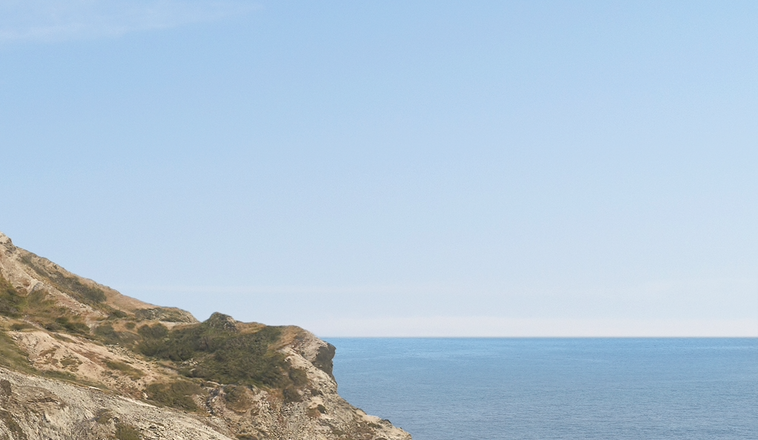
\includegraphics[width = 0.3\linewidth]{Figures/placeholder.png}
    \caption{\todo{Include a plot of a spectrum from an LHC measurement? Something out of omc3, maybe the one in my sextupolar contribution to ampdet ATS note.}}
    \label{figure:example_spectrum}
    \end{center}
\end{figure}

In principle the \(\abs{f_{jklm}}\) may be determined by a comparison of the amplitude of various spectral lines.
In practice, some additional considerations need to be taken, as decoherence of a kicked beam can lead to a reduction in the amplitude of the spectral lines observed, or the fact that the contributions of different RDTs might not be distinct.
More details and examples of this method is given in the next section, \cref{section:betatron_coupling}, for the case of betatron coupling RDTs.

%----------------------------------------------------------------------------------------

\section{Betatron Coupling}
\label{section:betatron_coupling}

When the betatronic motion of particles in transverse planes are independent of each other, they are said to be \intro{uncoupled}.
In particle colliders such as the LHC this is the desired behaviour.
When these motions share a dependency, they are said to be \intro{coupled}, and one refers to this phenomenon as \intro{betatron coupling}.%, or linear coupling.
The transverse motions of particles in an accelerator may couple due to a variety of factors, with solenoid and skew quadrupole fields being the primary sources of linear coupling.

In the LHC the main contribution to coupling comes from unwanted skew quadrupolar fields.
These mostly arise from normal quadrupoles mounted with a rotation error with respect to the longitudinal axis, but also from field imperfection from other magnets and feed-down from higher order magnets.
An example of a skew quadrupole is given in \cref{figure:skew_quadrupole}.

\begin{figure}[!htb]
    \begin{center}
    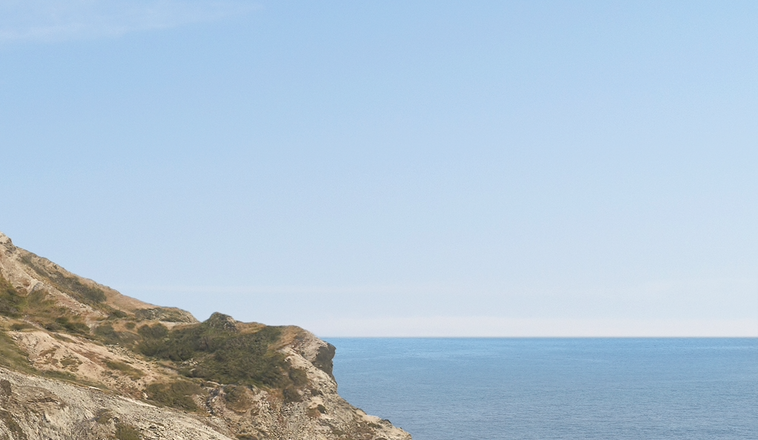
\includegraphics[width = 0.9\linewidth]{Figures/placeholder.png}
    \caption{\todo{Illustration of a skew quadrupole and its magnetic field lines.}}
    \label{figure:skew_quadrupole}
    \end{center}
\end{figure}

Betatron coupling needs to be kept under control as it can perturb the tune feedback systems and push tunes into resonances, or simply lead to a reduction in the dynamic aperture~\cite{PA:Ripken:Impact_Linear_Coupling_Nonlinear_Dynamics}.

\subsection{Parametrization of Betatron Coupling}
\label{subsection:parametrization_of_betatron_coupling}

There are different ways to parametrize coupled motion on a particle accelerator, the two most common being the Edwards-Teng~\cite{IEEE:Edwards:Parametrization_Linear_Coupled_Motion} and Mais-Ripken~\cite{AIP:Willeke:Methods_Beam_Optics} parametrization.
For coupled motion, a dependency between the horizontal and vertical planes is introduced.
As such, the transverse motions can no longer be described by two independent \(2 * 2\) matrices.
Instead, it is described by a \(4 * 4\) matrix \(\hat{\mathbf{M}}\):

\begin{equation}
    \hat{\mathbf{M}} = \left(
        \begin{array}{ll}
            \mathbf{P} & \mathbf{p} \\
            \mathbf{q} & \mathbf{Q}
    \end{array} \right) \text{ ,}
    \label{equation:coupled_motion_matrix}
\end{equation}
where \(\mathbf{P}\), \(\mathbf{p}\), \(\mathbf{q}\) and \(\mathbf{Q}\) are \(2 * 2\) matrices.
In the absence of betatron coupling, it follows that \(\mathbf{p}\) and \(\mathbf{q}\) are \num{0}.

In the Edwards-Teng parametrization presented in~\cite{IEEE:Edwards:Parametrization_Linear_Coupled_Motion}, the linear coupling is described by a symplectic rotation \(\mathbf{R}\) of \(\hat{\mathbf{M}}\) into its normal modes form \(\overline{\mathbf{M}}\), as shown in \cref{equation:edwards_teng_parametrization}.
In this frame the motion is decoupled.

\begin{equation}
    \overline{\mathbf{M}} = \left(
        \begin{array}{cc}
            \mathbf{X} & 0 \\
            0 & \mathbf{Y}
    \end{array} \right) = \mathbf{R} \hat{\mathbf{M}} \mathbf{R}^{-1} \text{ .}
    \label{equation:edwards_teng_parametrization}
\end{equation}

Edwards and Teng characterized the transformation \(\mathbf{R}\) by the symplectic matrix:

\begin{equation}
    \mathbf{R} =\left(
        \begin{array}{cc}
            \mathbf{I} \cos \theta & -\mathbf{K}^{-1} \sin \theta \\
            \mathbf{K} \sin \theta & \mathbf{I} \cos \theta
    \end{array} \right) \text{ ,}
    \label{equation:edwards_teng_rotation_matrix}
\end{equation}
where \(\mathbf{I}\) is the \(2 * 2\) unit matrix and \(\mathbf{K}\) is a \(2 * 2\) symplectic matrix, such that \(det(\mathbf{K}) = 1\).
The coupled motion may then be described by the uncoupled Twiss parameters seen in \cref{subsection:equations_of_motion_and_twiss_parameters}, together with the elements of matrix \(\mathbf{K}\) and Teng's angle of rotation \(\theta\).
In the case that \(\theta = 0\), the matrix \(\mathbf{R}\) is the identity matrix and as a result it will not rotate any of the modes: this corresponds to uncoupled motion.

The Edwards-Teng parameterization is used in the MAD-X~\cite{CODE:MADX_guide} code when handling of coupled motion.
In MAD-X the relevant parameters are \(\beta_{x, y}\), \(\alpha_{x, y}\), \(\mu_{x, y}\), \(\gamma_{x, y}\) and \(r_{11}\), \(r_{12}\), \(r_{21}\), \(r_{22}\), where \(r_{11} \ldots r_{22}\) correspond to the elements of \(\mathbf{K}\) multiplied by \(\tan \theta\).

The approach of Mais and Ripken was developed in~\cite{REPORT:Ripken:AllGerman} and is more accessible in~\cite{AIP:Willeke:Methods_Beam_Optics, REPORT:Borchardt:Calculation_Beam_Envelopes}.
It defines so-called \intro{Ripken parameters} \(\beta_{kj}, \alpha_{kj}\) and \(\gamma_{kj}\), where \(k = 1 \ldots 3\) refers to the plane (\(x, y, \ldots\)) and the index \(j\) refers to the eigenmodes, that are accurate in the presence of coupling.
In the coupled case, all \(\beta_N\) are non-zero and \(\beta_{11}, \beta_{22}\) are distinctively different from \(\beta_x, \beta_y\), respectively.
The relations linking these new parameters to the Twiss parameters can be found in~\cite{IOP:Lebedev:Betatron_Motion_Coupling}.
The Mais-Ripken parameterization is the basis of the Polymorphic Tracking Code's (PTC~\cite{CODE:Schmidt_Forest:PTC}) handling of coupled dynamics. 

\todo{Give a coupled phase space ellipse figure, like Ewen?}

\subsection{Coupled Motion}
\label{subsection:coupled_motion}

In the first order, according to \cref{equation:resonance_condition}, linear coupling drives two resonances: \(Q_x + Q_y = p\) and \(Q_x - Q_y = p\), with \(p \in \mathcal{Z}\).
These are called the \intro{sum and difference resonances}, respectively, and in their vicinity the beam dynamics are heavily influenced.
To higher order betatron coupling may also give stationary terms in the Hamiltonian (a tune shift), driving the \(2 Q_x\) and \(2 Q_y\) resonances, but these effects are typically negligible.

The impact of linear coupling on the beam motion has been studied through Hamiltonian perturbation theory~\cite{PHREV:Guignard:Betatron_Coupling_Radiation,BOOK:Wiedemann:Particle_Accelerator_Physics} and through the normal form / resonance driving term formalism~\cite{PHD:Franchi}.

As the transverse tunes approach the difference resonance, the emittance is described by:

\begin{equation}
    \varepsilon_x + \varepsilon_y = \mathrm{const} \text{ ,}
    \label{equation:coupled_emittances}
\end{equation}
and as the resonance is approached the beam motion may not become unstable.
Instead, there is a periodic exchange of emittance between the transverse planes, which leads to a beating in the betatron oscillation amplitudes.

The relation between the \intro{unperturbed tunes} \(Q_{x,y}\) and the \intro{coupled tunes} \(Q_{1,2}\) is given by~\cite{CAS:Bryant:Theory_Weak_Betatron_Coupling}:

\begin{equation}
    \begin{aligned}
        Q_1 &= Q_x- \frac{\Delta}{2} + \frac{\sqrt{\Delta^2 + \left| C^{-} \right|}}{2} \text{ ,} \\
        Q_2 &= Q_y+ \frac{\Delta}{2} - \frac{\sqrt{\Delta^2 + \left| C^{-} \right|}}{2} \text{ ,}
    \end{aligned}
    \label{equation:unperturbed_tunes_to_coupled_tunes}
\end{equation}
with \(\Delta\) being the unperturbed fractional tune split and \AbsCminus the linear coupling coefficient, a parameter describing the strength of the coupling.

When \(\Delta \gg \left| C^{-} \right|\), away from the resonance, the observed oscillations modes \(Q_{1,2}\) are almost identical to the uncoupled horizontal and vertical tunes \(Q_{x,y}\).
When the tunes are moved closer together, approching the difference resonance, the perturbed tunes are forced apart by the coupling and a minimal tune separation \(\Delta Q_{\mathrm{min}}\) can be observed.
The \AbsCminus of \cref{equation:unperturbed_tunes_to_coupled_tunes}, named the \intro{closest tune approach}, corresponds this separation.
\Cref{figure:closest_tune_approach} shows an illustration of the phenomenon in the vicinity of the resonance, where both the unperturbed and coupled fractional tunes are plotted against the uncoupled tune split.

\begin{figure}[!htb]
    \begin{center}
    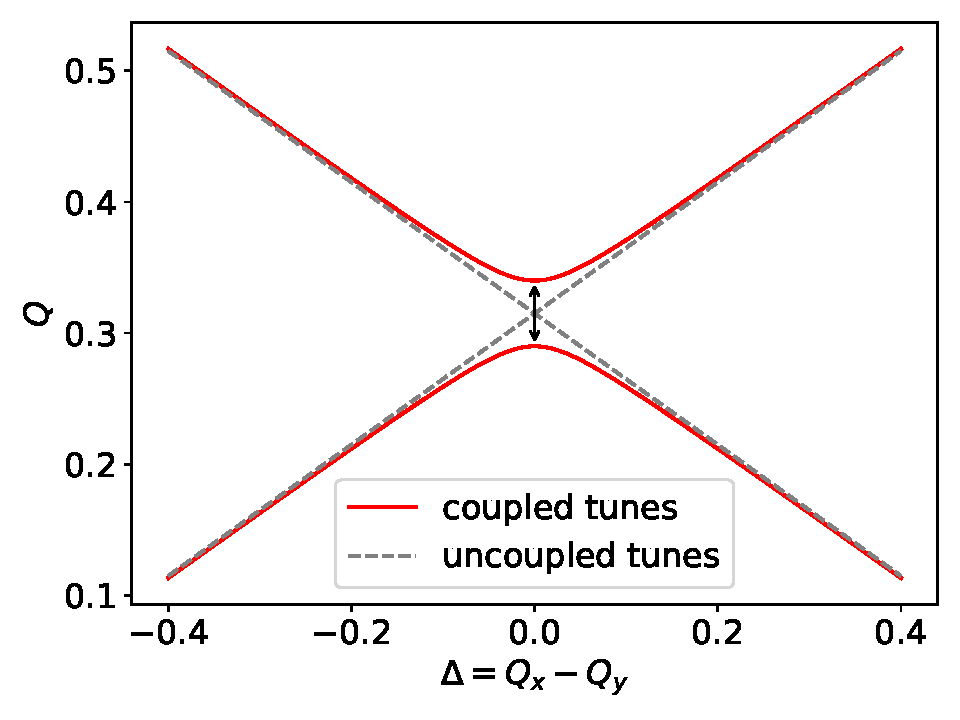
\includegraphics[width = 0.9\linewidth]{Figures/Beam_Dynamics_Theory/tune_perturbation.pdf}
    \caption{Illustration of coupled and uncoupled fractional tunes versus the uncoupled tune split. \todo{GET THE ONE FROM JACQUELINE?}}
    \label{figure:closest_tune_approach}
    \end{center}
\end{figure}

\subsection{Linear Coupling Resonance Driving Terms}
\label{subsection:measurement_coupling_rdts}

\todo{Can refer to~\cite{PRAB:Franchi:First_Simultaneous} for table with many RDTs.}


%----------------------------------------------------------------------------------------

\section{Luminosity}
\label{section:luminosity}

\todo{https://cds.cern.ch/record/1533084/files/CERN-THESIS-2013-022.pdf}

%----------------------------------------------------------------------------------------
\chapter{Optics Measurements and Corrections at the LHC}
\label{chapter:lhc_omc} % For referencing the chapter elsewhere, use \cref{chapter:lhc_omc}

The Large Hadron Collider (LHC) is a \qty{26.659}{\kilo\metre} synchrotron collider located at the European Center for Nuclear Research (CERN), on the French-Swiss border.
It is part of CERN's Accelerator Complex, illustrated in \cref{figure:cern_accelerator_complex}, a chain of particle accelerators progressively bringing protons and heavy ions up to an energy of \qty{6.8}{\tera\electronvolt} per beam, as of \num{2023}.

\begin{figure}[!htb]
  \centering
  \includegraphics*[width=0.9\linewidth]{Figures/Optics_Measurements_Corrections_at_LHC/cern_accelerator_complex.png}
  \caption{The CERN Accelerator Complex in \num{2022}, not to scale~\cite{Website:CERN_Accelerator_Complex_Resource}. For typical LHC operation, a proton beam is produced in \(\mathrm{LINAC}\)~\num{4} and follows the chain: \(\mathrm{LINAC}\)\num{4} \(\rightarrow\) \(\mathrm{PSB}\) \(\rightarrow\) \(\mathrm{PS}\) \(\rightarrow\) \(\mathrm{SPS}\) \(\rightarrow\) \(\mathrm{LHC}\).}
  \label{figure:cern_accelerator_complex}
\end{figure}

Accelerated particles go through a chain of different particle accelerators before reaching their experimental destinations.
For protons colliding in the LHC, the first step is a linear accelerator, LINAC\num{4}, which accelerates them up to a kinetic energy of \qty{160}{\mega\electronvolt}.
Next, the protons are injected into the Proton Synchrotron Booster (PSB), where they are accelerated to an energy of \qty{1.4}{\giga\electronvolt}.
The next stage is the Proton Synchrotron, in which they will reach \qty{25}{\giga\electronvolt}; then the Super Proton Synchrotron (SPS) where they are accelerated to \qty{450}{\giga\electronvolt}, when they are finally injected into the LHC.

The LHC circulates two counter-rotating hadron beams, each in their ring, which are made to collide at four Interaction Points (IPs) to provide data for High Energy Physics (HEP) experiments.
The main data-taking experiments on the LHC are ATLAS~\cite{ATLAS_Paper,Website:ATLAS,Website:ATLAS_CDS}, LHCf~\cite{LHCf_Paper,Website:LHCf,Website:LHCf_CDS}, ALICE~\cite{ALICE_Paper,Website:ALICE,Website:ALICE_CDS}, CMS~\cite{CMS_Paper,Website:CMS,Website:CMS_CDS}, TOTEM~\cite{TOTEM_Paper,Website:TOTEM,Website:TOTEM_CDS}, LHCb~\cite{LHCb_Paper,Website:LHCb,Website:LHCb_CDS} and MoEDAL~\cite{MoEDAL_Paper,Website:MOEDAL,Website:MOEDAL_CDS}.
The LHC is currently the world's highest-energy hadron colliding machine, colliding beams at \qty{13.6}{\tera\electronvolt} center-of-mass energy as of Run~\num{3}, \num{2023}.

%----------------------------------------------------------------------------------------

\section{The LHC Lattice}
\label{section:lhc_lattice}

The LHC lattice consists of eight \intro{octants} each intersected by an \intro{Insertion Region} (IR).
Conventionally, the segment between two \IRs is called an \intro{arc} and the arc between IR1 and IR2 is named Arc12, and similarly for other arcs.
An octant is defined as going from mid-arc to mid-arc around a given \IR which is located at its center.
Each octant is named according to the \IR at its center: the octant with \(\mathrm{IR1}\) at its center is named Octant1, and similarly for other octants.
An illustration and a detailed description on naming conventions can be found in \cref{appendix:naming_conventions}.
% The \IRs host either an \intro{Interaction Point} (IP) where beams are made to collide (ATLAS at IP1, ALICE at IP2, CMS at IP5 and LHCb at IP8) or important instrumentation (momentum cleaning at IR3, Radio-Frequency cavities at IR4, beam dump system at IR6 and betatron cleaning at IR7).

\begin{figure}[!h]
  \centering
  \includegraphics*[width=0.65\linewidth]{Figures/Optics_Measurements_Corrections_at_LHC/lhc_schematic.pdf}
  \caption{Schematic of the LHC layout, adapted from~\cite{PHD:Poyet}.}
  \label{figure:lhc_schematic_layout}
\end{figure}

Beam~\num{1} rotates clockwise in its ring when viewing the LHC from above, and Beam~\num{2} rotates counter-clockwise as viewed from above.
The beams occupy separate apertures, or beam pipes, except in the \IRs where they are eventually made to collide.
The layout of the LHC can be seen in simplified schematic form in~\cref{figure:lhc_schematic_layout}, and full details can be found in the LHC Design Report~\cite{BOOK:Bruning:LHC_Design_Report_Main_Ring,BOOK:Bruning:LHC_Design_Report_Infrastructure,BOOK:Benedikt:LHC_Design_Report_Injector_Chain}.

\subsection{The LHC Arcs}
\label{subsection:lhc_arcs}

Each arc in the LHC is made up of 23 cells and is approximately \qty{2.45}{\kilo\meter} long.
The layout of an LHC arc cell is given in~\cref{figure:lhc_schematic_arc_cell}, and a clearer schematic representation can be found in~\cite{MASTERS:Keintzel:Arc_Cell_Options_HELHC}.
The cell is based on a FBDB (FODO with Bends) layout alternating focusing and defocusing quadrupoles interspaced with dipoles.
These elements are all superconducting and are commonly labeled \intro{MQF}, \intro{MQD} and \intro{MB}, respectively.
% Details on equipment codes can be found at~\cite{CERN:Equipment_Codes}.

\begin{figure}[!hbt]
  \centering
  \includegraphics*[width=0.99\linewidth]{Figures/Optics_Measurements_Corrections_at_LHC/lhc_schematic_arc_cell.png}
  \caption{Schematic of an LHC arc cell~\cite{BOOK:Bruning:LHC_Design_Report_Main_Ring}.}
  \label{figure:lhc_schematic_arc_cell}
\end{figure}

Each cell contains two \intro{MQ} (one MQF, one MQD) with three MB in between, for a total of 6 MBs per cell.
The MBs are all powered in series and, for size constraint reasons~\cite{BOOK:Bruning:LHC_Design_Report_Main_Ring}, are of a dual bore design.
The MQs are themselves also powered in series but split in two families: one power circuit is dedicated to MQF magnets and another circuit for the MQD magnets, where each arc holds a circuit for each family.
As a consequence, these elements can only be trimmed in groups.
% A cross-section of the main LHC dipole assembly is given in~\cref{figure:lhc_main_dipole_cross_section}

% \begin{figure}
%   \centering
%   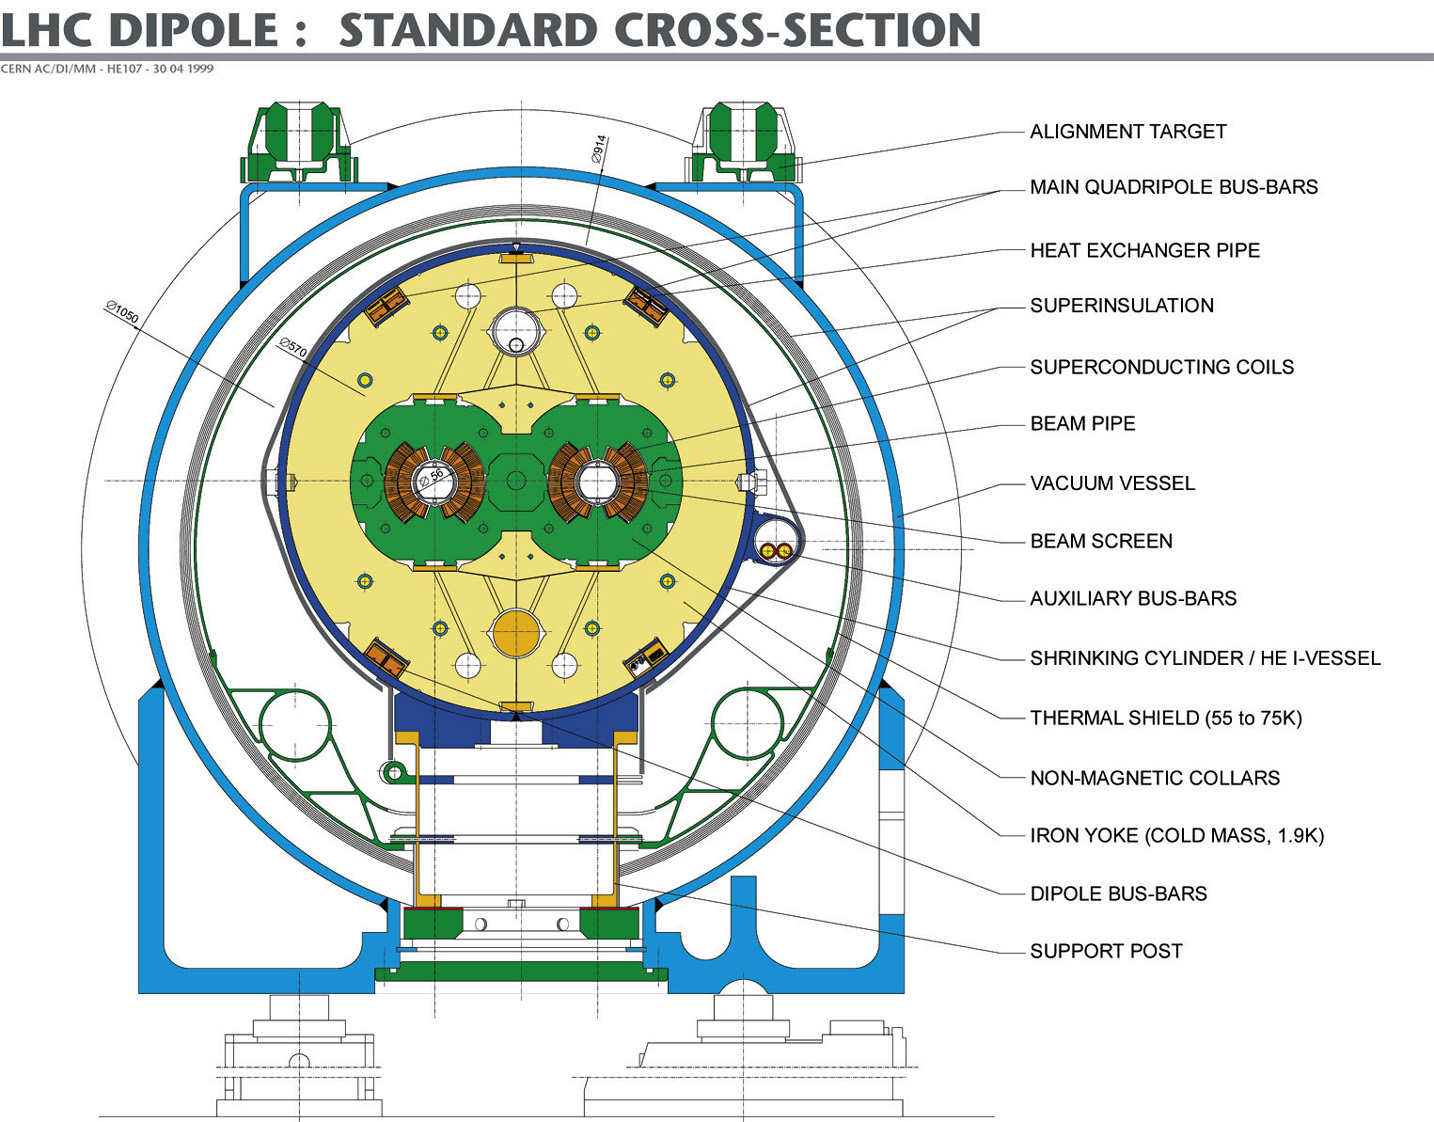
\includegraphics[width=0.85\linewidth]{Figures/Optics_Measurements_Corrections_at_LHC/lhc_main_dipole_cross_section.jpeg}
%   \caption{Cross-section of the LHC main dipole assembly~\cite{CERN:AC_Team:LHC_Dipole}.}
%   \label{figure:lhc_main_dipole_cross_section}
% \end{figure}

As a part of the main assemblies are superconducting \intro{spool piece magnets}, correctors used for the local compensation of magnetic errors in the main arc magnets~\cite{BOOK:Bruning:LHC_Design_Report_Main_Ring}.
These include sextupolar correctors, sextupolar spool pieces named \intro{MCS} and mounted on the ends of every main dipole, used to correct \(b_3\) errors of the MBs.
Similarly, octupole and decapole spool pieces are included and used for the compensation of \(b_4\) and \(b_5\) errors in the main arc magnets.
The octupole correctors are named \intro{MCO} while the decapole correctors are named \intro{MCD}, and both are nested together in an assembly named \intro{MCDO} which is mounted on the end of every second MB.
The spool piece magnets in the LHC are single aperture and powered in series similarly to the MQs, with one circuit assigned for each magnet family.

In addition to spool piece magnets, linear and nonlinear \intro{lattice correctors} are mounted on the main arc quadrupoles MQs.
These lattice correctors are powered in series per family, and independently for each beam.
Horizontal and vertical orbit correctors, respectively \intro{MCBH} and \intro{MCBV}, are installed at each focusing and defocusing MQ.
Normal trim quadrupoles, named \intro{MQT}, are primarily used for tune correction.
In each arc four MQTs are rotated by \qty{45}{\degree} to form skew quadrupoles, named \intro{MQS}, used for linear coupling correction.
Normal and skew sextupoles \intro{MS} and \intro{MSS}, used for natural chromaticity and chromatic coupling correction respectively, are mounted on the MQs.
Landau octupoles \intro{MO} provide damping of coherent oscillations, and are split into two families (focusing and defocusing) powered in series, such that there are two families per arc and per beam.

\Cref{figure:lhc_arc_cell_latwiss} shows a simplified layout of an LHC arc cell's elements as well as \(\beta\) and dispersion functions for \num{2022} optics at \(\beta^{\ast} =\) \qty{30}{\centi\meter}.
In the layout part of the plot element powerings are indicated, with MBs in \textcolor{latwiss_blue}{blue}, MQs in \textcolor{latwiss_red}{red}, MSs in \textcolor{latwiss_yellow}{yellow}, MOs in \textcolor{latwiss_green}{green} and beam position monitors (BPMs) as grey patches.
Note that not all elements are indicated there.
\Cref{figure:lhc_arc23_latwiss} shows a similar plot but across LHC arc\num{23} for the same optics.

\begin{figure}[!hbt]
  \centering
  \includegraphics*[width=0.99\linewidth]{Figures/Optics_Measurements_Corrections_at_LHC/lhc_arc_cell.pdf}
  \caption{Simplified layout and optics functions in an LHC arc cell for \(\beta^{\ast} =\) \qty{30}{\centi\meter} optics.}
  \label{figure:lhc_arc_cell_latwiss}
\end{figure}

\begin{figure}[!hbt]
  \centering
  \includegraphics*[width=0.99\linewidth]{Figures/Optics_Measurements_Corrections_at_LHC/lhc_arc23.pdf}
  \caption{Simplified layout and optics functions in LHC arc\num{23} for \(\beta^{\ast} =\) \qty{30}{\centi\meter} optics.}
  \label{figure:lhc_arc23_latwiss}
\end{figure}

The purpose of the arcs is that of beam transport to the more specific parts of the machine.

\subsection{The LHC Experimental Interaction Regions}
\label{subsection:lhc_eirs}

In the middle of each octant, in between arcs, the LHC hosts \intro{long straight sections} (see \cref{appendix:naming_conventions} for details) with specific purposes.
Each of these is centered around an Insertion Region where a dedicated layout is in place to fulfill the section's purpose.
The purpose of each straight section is briefly stated on \cref{figure:lhc_schematic_layout} and detailed in \cref{table:lhc_straight_sections}.

\begin{table}[!hbt]
  \centering
  \begin{tblr}{colspec={cc}}
      \hline
      \text{Straight Section} & \text{Description}                                 \\
      \hline
      IR\num{1}               & ATLAS and LHCf Experiments                           \\
      IR\num{2}               & ALICE Experiment and B\num{1} Injection              \\
      IR\num{3}               & Momentum Cleaning (Collimation)                      \\
      IR\num{4}               & RF Systems and LHC Instrumentation                   \\
      IR\num{5}               & CMS and TOTEM Experiments                            \\
      IR\num{6}               & Beam Dump System                                     \\
      IR\num{7}               & Betatron Cleaning (Collimation)                      \\
      IR\num{8}               & LHCb and MoEDAL Experiments, and B\num{2} Injection  \\
      \hline
  \end{tblr}
  \caption{Description and purpose of the straight sections in the LHC}.
  \label{table:lhc_straight_sections}
\end{table}

Of interest to this thesis are the \intro{experimental insertions}, located in IR\num{1}, IR\num{2}, IR\num{5}, and IR\num{8}, where the beams are made to collide.
An insertion region in which beams are made to collide is called an \intro{Interaction Region}, or sometimes Experimental Interaction Region.
In this document, when using the short form IR, it is meant to refer to an Interaction Region.

At the center of the IR, beams are made to collide at the \intro{Interaction Point} (IP).
In order to achieve high luminosity during collisions, and as shown in \cref{section:luminosity}, the \(\beta\)-functions at the IPs are squeezed to very small values.
\Cref{figure:ir5_and_around} shows the \(\beta\)-functions in the LHC around IP5 at both injection and collision optics, where the squeeze is apparent.

\begin{figure}[!hbt]
  \centering
  \includegraphics*[width=0.99\linewidth]{Figures/Optics_Measurements_Corrections_at_LHC/ir5_surroundings_optics_2.pdf}
  \caption{The horizontal and vertical \betafunctions in the LHC around IP5 at injection optics (top) and collision optics (bottom). Notice the drastically different scales on the vertical axes.}
  \label{figure:ir5_and_around}
\end{figure}

During normal operation the \(\beta^{\ast}\) at ATLAS and CMS is very squeezed: \(\beta^{\ast} =\) \qty{30}{\centi\metre} during collisions as of \num{2023}.
For the configuration, at ALICE and LHCb the \(\beta^{\ast}\) are only squeezed to higher values, \qty{10}{\meter} and \qty{2}{\meter} respectively in \num{2023}.
During collisions involving ions (Pb-Pb and p-Pb) the \(\beta^{\ast}\) is reduced at ALICE and LHCb.
\Cref{table:lhc_betastars_configurations} summarizes the \(\beta^{\ast}\) values for the different experiments and configurations.

\begin{table}[!htb]
  \centering
  $\begin{tblr}{colspec={cccc}}
      \hline
      \SetCell[r=2,c=1]{m,c} \text{IP} & \SetCell[c=3]{c} \mathbf{\beta^{\ast}}                                                    \\
      \cline{2-4}
                                       &  \text{Injection Optics}  &  \text{Proton Collisions} &  \text{Ion Collisions}   \\
      \hline
      \text{IP\num{1}}                 &  \qty{11}{\meter}         &  \qty{30}{\centi\meter}   &  \qty{50}{\centi\meter}  \\
      \text{IP\num{2}}                 &  \qty{11}{\meter}         &  \qty{10}{\meter}         &  \qty{50}{\centi\meter}  \\
      \text{IP\num{5}}                 &  \qty{11}{\meter}         &  \qty{30}{\centi\meter}   &  \qty{50}{\centi\meter}  \\
      \text{IP\num{8}}                 &  \qty{11}{\meter}         &  \qty{2}{\meter}          &  \qty{50}{\centi\meter}  \\
      \hline
  \end{tblr}$
  \caption{Value of the \(\beta^{\ast}_{x,y}\) at different IPs for different optics configurations as of Run~\num{3}.}
  \label{table:lhc_betastars_configurations}
\end{table}

In order to achieve a small \(\beta^{\ast}\) at the IPs, the beams are focused using a superconducting \intro{triplet} of quadrupoles just before the IP, on either side~\cite{CERN:Ostojic:Improved_Optical_System_LHC_Triplet}.
The triplet is optimized to be symmetric~\cite{CERN:DAmico:Analysis_Generic_Insertions}, with Q\num{1} and Q\num{3} being the same length at \qty{6.3}{\meter} and Q\num{2} split into two sub-magnets Q\num{2}a and Q\num{2}b of \qty{5.5}{\meter} each.
All three magnets are powered in series but can be adjusted individually using dedicated trim converters~\cite{PAC:Bordry:LHC_Inner_Triplet_Powering}.

This arrangement of three quadrupoles allows for a stong focusing of the \(\beta\)-functions in both transverse planes.
However, such an arrangement leads to high \(\beta\)-functions in the triplet quadrupoles themselves and neighbouring elements.
An illustration of the area close to IP\num{5} for collision optics with \(\beta^{\ast} =\) \qty{30}{\centi\metre} is given in \cref{figure:lhc_ir5_zoomed}.

\begin{figure}[!hbt]
  \centering
  \includegraphics*[width=0.99\linewidth]{Figures/Optics_Measurements_Corrections_at_LHC/lhc_ir5_zoomed.pdf}
  \caption{The simplified elements layout and \(\beta\)-functions around IP\num{5} at collision optics, without crossing angles.}
  \label{figure:lhc_ir5_zoomed}
\end{figure}

On the layout plot the three \textcolor{latwiss_red}{red patches} closest to the IP location correspond to Q\num{1}, Q\num{2} and Q\num{3} respectively, the triplet quadrupoles.
The \textcolor{latwiss_blue}{blue patches} correspond to D\num{1} (first batch) and D\num{2} (outer dipole), the \intro{separation / recombination dipoles} responsible for bringing the beams together / apart in the common region from / to their separate apertures in the arcs.
The separation dipole D\num{1} is made of six \qty{3.4}{\meter} long normal conducting magnets while D\num{2} is a superconducting twin aperture magnet \qty{9.45}{\meter} long.
Further quadrupoles are matching quadrupoles and will be discussed later.
The grey lines correspond to the location of Beam Position Monitors (BPMs), measurement instrumentation.

Due to the large \(\beta\)-functions in the triplet quadrupoles, as can be seen in \cref{figure:lhc_ir5_zoomed}, any magnetic error in the elements of the IR would have a strong impact on the beam dynamics.
To enable correction of these errors, linear and non-linear corrector magnets are installed along the IR, distributed symmetrically around the IP: every corrector magnet on one side of the IP has a counterpart on the other side.
Of interest to this thesis are the a\num{2} skew quadrupole correctors installed just before Q\num{3} on each side of the IP, the locations of which are highlighted in \cref{figure:lhc_ir5_zoomed} by green vertical lines.
A schematic of the corrector layout is shown in \cref{figure:lhc_ir_corrector_layout}.
All correctors are individually powered magnets.
\todo{ARE THEY?}

\begin{figure}[!hbt]
  \centering
  \includegraphics*[width=0.92\linewidth]{Figures/Optics_Measurements_Corrections_at_LHC/corrector_package.png}
  \caption{Layout of the triplet magnets and the linear and nonlinear correctors in the LHC experimental insertions~\cite{CERN:Bruning:Dynap_Studies}, showing common aperture magnets. The skew quadrupole correctors correspond to order a\num{2} and are located in the C\num{2} package.}
  \label{figure:lhc_ir_corrector_layout}
\end{figure}

In order to prevent parasitic crossings between the two beams' bunches around the IP during collisions, \intro{separation bumps} are implemented in a single transverse plane for each IP, in the form of closed orbit bumps.
Due to the presence of these bumps, in order to reach collisions a \intro{crossing angle} is introduced.
The optics in IR\num{1} and IR\num{5} are identical except for the crossing schemes: the crossing angle is in the vertical plane at IR\num{1} and in the horizontal plane at IR\num{5}.
Respectively, the separation bumps are in the horizontal plane at IR\num{1} and in the vertical plane at IR\num{5}.
\Cref{figure:lhc_crossing_schemes_ip15} shows the crossing schemes for both IR\num{1} and IR\num{5} at collision optics, with the location of the triplets highlighted in grey and the that of the separation dipoles in yellow.

\begin{figure}[!hbt]
  \centering
  \includegraphics*[width=0.99\linewidth]{Figures/Optics_Measurements_Corrections_at_LHC/lhc_crossing_schemes_ip15.pdf}
  \caption{Crossing schemes for IR\num{1} and IR\num{5} at collision optics.}
  \label{figure:lhc_crossing_schemes_ip15}
\end{figure}

Other IRs, not of interest to this thesis, have significantly different layouts which can be found in details in~\cite{BOOK:Bruning:LHC_Design_Report_Main_Ring,PHD:Vanbavinckhove}.

\subsection{Matching Sections and Dispersion Suppressors}
\label{subsection:matching_sections_dispersion_suppressors}

Assuring the transition between the arcs and the specific optics conditions of the IRs are \intro{matching sections} and \intro{dispersion suppressors}, as can be seen on \cref{figure:ir5_and_around}.
Note that the area designated as matching section on the figure also includes the dispersion suppressor.
Together, the two segments are responsible for matching the TWISS functions between the arcs and the IRs, and for reducing the dispersion to near-zero value, respectively.

The dispersion suppressor is made of two arc cells containing two instead of the regular three dipoles.
The quadrupoles in these cells, Q\num{7} to Q\num{10}, are powered individually.
The dispersion suppressor leading to IP\num{5} can be seen on \cref{figure:lhc_dispersion_suppressor}, where the beam travels from left to right.

\begin{figure}[!hbt]
  \centering
  \includegraphics*[width=0.99\linewidth]{Figures/Optics_Measurements_Corrections_at_LHC/lhc_dispersion_suppressor.pdf}
  \caption{Simplified layout and optics functions in the dispersion suppressor leading beam \num{1} to IP\num{5}, for \(\beta^{\ast} =\) \qty{30}{\centi\meter} optics.}
  \label{figure:lhc_dispersion_suppressor}
\end{figure}

The matching section is made of three individually powered superconducting quadrupoles, Q\num{4} to Q\num{6}, used to match the TWISS functions from their out of the arcs to that at the entrance of the triplets.
In order to help the matching to the arc, the trim quadrupoles QT\num{11} to QT\num{13}, adjacent to the FODO quadrupoles Q\num{11} to Q\num{13}, are also individually powered and used for the matching.
The full segment, from the start of the dispersion suppressor to just before separation dipole D\num{2}, is shown in \cref{figure:lhc_matching_section}.

\begin{figure}[!hbt]
  \centering
  \includegraphics*[width=0.99\linewidth]{Figures/Optics_Measurements_Corrections_at_LHC/lhc_matching_section.pdf}
  \caption{Simplified layout and optics functions in the matching section leading beam \num{1} to IP\num{5}, for \(\beta^{\ast} =\) \qty{30}{\centi\meter} optics.}
  \label{figure:lhc_matching_section}
\end{figure}

\subsection{The ATS Optics Scheme}
\label{subsection:lhc_ats_optics_scheme}

When pushing the \(\beta^{\ast}\) to smaller values, and therefore the \(\beta\)-functions in the triplets to higher ones, the chromatic effects produced by the triplet quadrupoles~\cref{equation:natural_chromaticity_approximation} increase drastically and need to be corrected.
As the beam energy reaches its maximum, the beam size gets smaller and an aperture margin that allows to increase the \(\beta\)-functions appears in the arcs.

The \intro{Achromatic Telescopic Squeeze} (ATS) optics scheme~\cite{CERN:Fartoukh:ATS_Report,PRAB:Fartoukh:Achromatic_Telescopic_Squeeze,IPAC:Pojer:LHC_ATS_Experience} consists in splitting the reduction of the \(\beta^{\ast}\) (the squeeze) in two stages.
In the first one, the \intro{pre-squeeze}, the \(\beta^{\ast}\) is reduced using the matching quadrupoles around the affected IP.
As using these matching quadrupoles has several limits (magnet strength, chromaticity correction, orbit control), a second stage is necessary.
In this second stage, the \intro{tele-squeeze}, the \(\beta^{\ast}\) is reduced by using the matching quadrupoles in the nearby IRs: IR\num{2} and IR\num{8} for the tele-squeeze of IR\num{1}, and IR\num{4} and IR\num{6} for the tele-squeeze of IR\num{5}.
Sectors \numlist{81;12;45;56} are therefore called ATS sectors.
This modulation in the second stage sends \(\beta\)-beating waves down the arcs, which make the \(\beta\)-functions peak at the location of sextupoles and octupoles in the those arcs, enhancing their efficiency.

The ratio between the \(\beta^{\ast}\) at the end of the pre-squeeze (\(\beta^{\ast}_{Pre}\)) and the \(\beta^{\ast}\) at the end of the tele-squeeze (\(\beta^{\ast}_{Tele}\)) is called \intro{tele-index} and is denoted \(r_{Tele}\).
It is defined as:

\begin{equation}
  r_{Tele} = \frac{\beta^{\ast}_{Pre}}{\beta^{\ast}_{Tele}}
  \label{equation:tele_index}
\end{equation}

\Cref{figure:lhc_ats_scheme} shows the \(\beta\)-functions at \qty{6.5}{\tera\electronvolt} around IP\num{5}, where one can see the \(\beta\)-beating wave in the neighbouring ATS sectors \num{45} and \num{56}.

\begin{figure}[!hbt]
  \centering
  \includegraphics*[width=0.99\linewidth]{Figures/Optics_Measurements_Corrections_at_LHC/lhc_ats_wave.pdf}
  \caption{The \(\beta\)-functions in sectors \num{45} and \num{56} at different points in the squeeze for the \num{2022} optics: at the end of the pre-squeeze (top) and at the end of the tele-squeeze (bottom).}
  \label{figure:lhc_ats_scheme}
\end{figure}

This ATS optics scheme has been used in the LHC starting Run~\num{2} and allowed reducing the collision optics \(\beta^{\ast}\) from its design value of \qty{55}{\centi\meter} to \qty{30}{\centi\meter}.
It is the operational baseline of Run~\num{3}.

%----------------------------------------------------------------------------------------

\section{The Operational Cycle of the LHC}
\label{section:lhc_operational_cycle}

The LHC operational cycle~\cite{Report:LHCModes}, illustrated in \cref{figure:lhc_cycle}, begins with a \intro{pre-cycle} of certain magnetic elements~\cite{Report:LHCMagnetsPreCycles}.
During pre-cycle no beams are present in the rings and the respective element currents are increased up to several \unit{\tera\electronvolt} beam energy configuration, to ensure the reproducibility of the magnetic fields over successive fills.
The exact nature of the pre-cycle depends on the magnetic elements, and a pre-cycle is not necessarily performed before each fill.

After the pre-cycle comes the \intro{injection} stage: beams are injected from the Super Proton Synchrotron (SPS) at an energy of \qty{450}{\giga\electronvolt}.
First a probe beam consisting of just a few bunches is injected to check the validity of several systems (injection interlock, orbit, tune, chromaticity and coupling control), then a physics beam meant for collisions is injected.
At injection optics the \(\beta^{\ast}_{x,y}\) at the main colliding IPs (IP\num{1} and IP\num{5}) is \qty{11}{\metre}.
The number of bunches, their intensity and their filling pattern~\cite{Report:LHCStandardFillingSchemes} depends strongly on the experimental demands.
For optics measurements for instance, between one and three low intensity, non-colliding bunches of about \num{e10} protons per bunch are injected for each beam.
For luminosity production a larger number of high intensity bunches is injected: in the order of \num{e3} bunches, with \(\ge\) \num{e11} protons per bunch.

After injection, the beam energy is increased up to collision energy (\qty{6.8}{\tera\electronvolt} in Run~3) while the beams are squeezed and the \(\beta^{\ast}\) reduced.
This process, called \intro{combined ramp and squeeze}, has been used in the LHC since 2017~\cite{IPAC:Camillocci:CombinedRampAndSqueeze}.
Before then the squeezing process only started once the energy had reached collision value.

After reaching top energy, a configuration known as \intro{flat-top}, another \intro{squeeze} is performed to bring the \(\beta^{\ast}\) to collision value.
This is when the ATS scheme mentioned in \cref{subsection:lhc_ats_optics_scheme} happens.

In a final step before luminosity production, called \intro{adjust}, the last few needed parameters are adjusted to bring the beams into collision: tunes, crossing angles, collapse of the separation bumps.
This configuration called \intro{stable beams} is kept throughout the luminosity production for the fill.
The fill ends when the beams are extracted from the machine, a.k.a. \intro{beam dump}, after which the cycle ends by a \intro{ramp down} of the magnets' currents.

The working point is changed several times along the cycle for stability reasons.
As of \num{2022}, at injection the transverse tunes are (\(62.275, 60.293\)).
The working point is brought to (\(62.28, 60.31\)) during the ramp and squeeze, at the end of which it is moved again to (\(62.311, 60.318\)).
A final change is made in the adjust step, where the tunes are brought to (\(62.314, 60.319\)) before going into collisions.
This last setting may be changed by machine operators during stable beams in order to optimize for beam lifetime.

\begin{figure}[!hbt]
    \centering
    \includegraphics*[width=0.99\linewidth]{Figures/Optics_Measurements_Corrections_at_LHC/lhc_cycle.pdf}
    \caption{Simplified illustration of the LHC nominal cycle.}
    \label{figure:lhc_cycle}
\end{figure}

Starting in Run~\num{3}, some additional complexities were added to the cycle that are not shown in \cref{figure:lhc_cycle}.
In \num{2022} a \(\beta^{\ast}\)-leveling was introduced, were collisions start at a \(\beta^{\ast}\) of \qty{60}{\centi\meter} and the \(\beta^{\ast}\) is progressively reduced to \qty{30}{\centi\meter} during stable beams.
This is done in order to limit pile-up for the experiments (at around \num{52} events per bunch crossing for the main IPs) and the impact on the triplets' cryogenics capacity~\cite{CERN:Fartoukh:LHC_Config_Run3, CERN:Ferlin:Cryogenics}.
This \(\beta^{\ast}\)-leveling is moved to start at \(\beta^{\ast} =\) \qty{1.2}{\meter} in \num{2023} and \num{2024}, with a higher pile-up value.
Starting in \num{2023} an anti-telesqueeze is performed in the ramp to help the forward physics experiments, and a crossing-angle rotation at LHCb (IP\num{8}) is done when reaching flat-top in order to maintain physics conditions at the IP regardless of the LHCb spectrometer polarity~\cite{CERN:Fartoukh:LHC_Config_Run3}.

%----------------------------------------------------------------------------------------

\section{Optics Measurements and Corrections}
\label{section:optics_measurements_and_corrections}

The quality of the LHC optics has a significant impact on the machine's performance.
For instance, the luminosity achieved by the machine is directly determined by the \(\beta\)-functions at the IPs, as seen in \cref{section:luminosity}.
Furthermore, a good control of the \(\beta\)-functions is essential for safe beam operations due to the destructive power of the LHC beams, and the machine is subject to strict limits on the deviation from model values~\cite{CERN:Bruning:Field_Quality_Spec_LHC_Main_Dipoles}.
One can then define the \intro{beta-beating}, a good indicator of the quality of the linear optics, as the relative deviation of the machine's \(\beta\)-functions from that of the designed values.
It is defined as:

\begin{equation}
  \frac{\Delta \beta_z(s)}{\beta_z(s)} = \frac{\beta_z(s)_{\mathrm{measured}} - \beta_z(s)_{\mathrm{model}}}{\beta_z(s)_{\mathrm{model}}} \quad \text { where } z = x, y \text{ .}
  \label{equation:beta_beating_definition}
\end{equation}

In order to verify the machine's beam optics and find any potential faults, or deviations from the model values, beam measurements are necessary.
From these, comparisons to model values are made which allow for an assessment and understanding of the errors in the machine; and corrections can be calculated and applied to bring back the optics as close to the nominal scenario as possible.
As the linear optics functions impact the non-linear phenomenology of an accelerator, a well understood and corrected linear optics a pre-requisite to study of the non-linear dynamics.
\Cref{figure:virgin_vs_corrected_lhcb2} shows the \(\beta\)-beating for beam~\num{2} of the LHC in its \num{2022} virgin\footnote{The term \textit{virgin} refers to the state of the machine without any corrections.} state and with all determined corrections trimmed in, at the end of the commissioning phase.
Correction of the linear optics functions towards their nominal values also leads to an enhanced rms closed orbit around the ring since the orbit feedback algorithms in the LHC assume the nominal LHC model~\cite{PRAB:Tomas:Record_Low_Beta_Beating_in_the_LHC, PRAB:Persson:LHC_Optics_Commissioning_OnePercent}.

\begin{figure}[!hbt]
  \centering
  \includegraphics*[width=0.9\linewidth]{Figures/Optics_Measurements_Corrections_at_LHC/virgin_vs_commissionned_lhcb2.pdf}
  \caption{The measured \(\beta\)-beating at the beginning (\textcolor{mplblue}{blue}) and end (\textcolor{mplorange}{orange}) of the LHC \num{2022} commissioning, for beam \num{2}.}
  \label{figure:virgin_vs_corrected_lhcb2}
\end{figure}

\subsection{Beam Instrumentation for Optics Measurements}
\label{subsection:beam_instrumentation_for_optics_measurements}

Circular machines such as the LHC include a variety of beam instrumentation devices which serve various purposes, from injection kickers and feedback systems used in regular operations to dedicated devices for optics measurements.

\subsubsection*{Beam Position Monitors and Tune Measurement}

\intro{Beam Position Monitors} (BPMs) are one of the most crucial devices for beam diagnostics.
They measure the transverse center of charge of circulating bunches, either in a given plane for single plane BPMs, or in both planes simultaneously for dual plane BPMs.
In the LHC, this centroid beam position can be measured on a turn-by-turn and bunch-by-bunch basis by around \num{500} dual plane BPMs across the machine.
So-called stripline BPMs are employed in the common apertures as they can discriminate between counter-rotating bunches, while button BPMs are used in the remaining portions of the machine~\cite{BOOK:Bruning:LHC_Design_Report_Main_Ring}. 
The location of BPMs in the lattice can be seen as vertical grey lines, in an insertion region such as IR\num{5} in \cref{figure:lhc_ir5_zoomed,figure:lhc_matching_section} and in the arcs in \cref{figure:lhc_arc_cell_latwiss}.

% Measurement of the tune can be done in different ways.
% One way consists at measuring transverse oscillations and looking at the spectrum of these oscillations.
In the LHC, the \intro{Base Band Tune} (BBQ) system~\cite{CERN:Boccardi:LHC_Transverse_Diagnostics_Systems,CERN:Boccardi:LHC_BBQ_Tune_Chromaticity_Systems} provides continuous, passive monitoring of the tune by performing spectral analysis of the orbit data at a specific location in IR\num{4}.
The BBQ is also capable of measuring an estimation of the linear coupling at the measurement location, which can be used as a rough first estimate for the coupling in the machine.
While it is possible to assess tune and coupling with the BBQ without external excitation of the beam, the LHC chirp can generate small transverse oscillations to improve the quality of these measurements.

\subsubsection*{Experimental Kickers}

For the study of beam dynamics, measurements are done by inducing large transverse oscillations of the beam to be picked up by the BPMs, typically much larger than natural beam size. 
Large oscillation amplitudes are required to provide a good signal-to-noise ratio 
The spectral analysis of measured turn-by-turn positions provides valuable insights in all the modes contained in the particle motion, at each BPM location.
In the LHC kicker dipole magnets are available for both beams, located in IR\num{4}.
These magnets can operate in three possible modes, referred to as the \intro{Tune Kicker} (MKQ), \intro{Aperture Kicker} (MKA), and the \intro{AC Dipole}.

The tune and aperture kickers~\cite{CERN:Barlow:Control_MKQA_LHC,IPMS:Carlier:Kicker_Pulse_Generator_Measurement_Tune_Dynamic_Aperture_LHC} operate as traditional kicker magnets: ramping up and down in a single turn, applying a transverse kick to the beam and then allowing free motion.
The name only refers to the amplitude of induced oscillations: lower strength to measure the tune and higher strength to measure the available dynamic aperture.
Unfortunately, at top energy the amplitude of oscillations achievable with the kickers is considerably reduced, and the beam will decohere after being kicked: the momentum distribution of particles in the bunch will cause the observed centroid of the beam to show a decaying oscillation~\cite{Report:Meller:Decoherence_Kicked_Beams}.
This decoherence will lead to emittance increase.
As a consequence a beam can only be kicked a certain number of times before needing to be replaced, and it can take up to several hours to reach the same machine configuration again, as seen in \cref{section:lhc_operational_cycle}.

For optics measurements lasting oscillations are preffered, as they increase the spectral resolution and reduce noise floor in the spectral analysis of turn-by-turn data.
Furthermore, a non-destructive excitation method is preferred in order not to alter the beam state, which allow repeated measurements.

Such a non-destructive, sustained excitation of the beams can be achieved with the AC Dipole.
It is a fast oscillating dipole magnet which can generate forced driven oscillations with large amplitudes by exciting the beam at frequencies close to the natural tunes~\cite{PHD:Miyamoto,CERN:Serrano:LHC_ACDipole_Introduction}.
Moreover, the AC Dipole strength can be ramped up and down adiabaticity~\cite{PRAB:Tomas:Adiabaticity_Ramping_Process_AC_Dipole} and kept constant at high amplitudes, allowing for a long lasting coherent oscillations of the beam.
These properties, fullfilling the aforementioned requirements, make the AC Dipole the most important tool for optics measurements in the LHC.
A comparison of the turn-by-turn data obtained from beam excitation with a single free kick and an AC Dipole is shown in \cref{figure:kick_vs_acdipole_tbt}.

\begin{figure}[!htb]
  \centering
  \includegraphics*[width=0.99\linewidth]{Figures/Optics_Measurements_Corrections_at_LHC/kick_vs_acdipole.pdf}
  \caption{Comparison of turn-by-turn data obtained from a single free kick (top) and an AC Dipole excitation (bottom).}
  \label{figure:kick_vs_acdipole_tbt}
\end{figure}

\subsection{Optics Measurements}
\label{subsection:optics_measurements}

Optics measurements are performed by exciting the beam and analyzing the resulting betatron oscillations.
The various steps of the measurement process are described below.

\subsubsection*{Beam Excitation}

The first step of optics measurements in the LHC is to excite the beams with the AC Dipole.
As excitation of the beams to large amplitudes can represent a risk to the safety of the machine, such measurements are only performed with a single low intensity bunch of about \num{e10} protons.
In the LHC, the AC Dipole has a ramp-up and ramp-down time of \num{2000} turns, and is able to drive excitations at maximum strength for \num{6600} turns before ramping down, as can be seen on \cref{figure:kick_vs_acdipole_tbt}.
When exciting the beam, the turn-by-turn position of the bunch is measured by the BPMs across the machine and only the turns corresponding to the maximum AC Dipole strength are used for analysis.

It is important to note now that the forced oscillations introduce a perturbation on the optics.
In the case of free oscillations, it was shown in \cref{chapter:Theory} that the transverse motion goes according to \cref{equation:hill_solution}.
Using the horizontal plane as example from now on, and considering \(\phi_{x,0} = 0\) at the start of machine:

\begin{equation}
  x(s) = \sqrt{2 J_x \beta_x(s)} \cos \left( \phi_x \right) \text{ ,}
\end{equation}
with \(\phi_x\) and \(J_x\) the action and angle variables respectively.

When the AC Dipole is driving the beam, an equivalent parametrization exists, and noting \(x_D(s)\) the horizontal driven coordinate one can express it as~\cite{PHD:Miyamoto,PRAB:Tomas:Normal_Form_Particle_Motion_AC_Dipole}:

\begin{equation}
  x_D(s)=\sqrt{2 J_x \beta_x(s)} \cos \left( \phi_x \right) + \sqrt{2 A \beta_{D,x}(s)} \cos \left( \phi_D \right) \text{ ,}
  \label{equation:driven_transverse_motion}
\end{equation}
where \(A\) and \(\phi_D\) are respectively the action and angle variables of the forced oscillations, and \(\beta_{D,x}(s)\) is the \(\beta\)-function modified by the AC Dipole.
The form of \cref{equation:driven_transverse_motion} makes the assumption that the forced oscillation term only depends on \(\phi_D\).

The \(\beta\)-function modified by the AC Dipole, corresponding to the perturbed optics under forced oscillations, is given as~\cite{PRAB:Miyamoto:Parametrization_Driven_Betatron_Oscillation}:

\begin{equation}
  \beta_{D,x}(s) = \frac{1 + \lambda_D^2 - 2 \lambda_D \cos \left(\psi_D\right)}{1 - \lambda_D^2} \beta_x(s) \text{ ,}
  \label{equation:driven_beta_function}
\end{equation}
where \(\psi_D\) is the phase advance with respect to the AC Dipole location and the relation is valid for both horizontal and vertical \(\beta\)-functions.
The \(\lambda_D\) term is dependent on the gap between the driven and natural tune, and is defined by~\cite{PRAB:Miyamoto:Parametrization_Driven_Betatron_Oscillation}:

\begin{equation}
  \lambda_D = \frac{\sin \left(\pi \delta_D \right)}{\sin \left(2 \pi Q_x + \pi \delta_D \right)} \text{ ,}
  \label{equation:driven_oscillations_lambda_D}
\end{equation}
in which \(\delta_D = Q_D - Q\) corresponds to the aforementioned gap.
In the LHC the AC Dipole is usually driven with \(\delta_{D,x} = -0.01\) and \(\delta_{D,y} = 0.012\).

One can see in \cref{figure:acdipole_beta_functions_vs_nominal} the impact of an AC Dipole on the vertical \(\beta\)-function in a simple FODO lattice, where the difference between the free and forced cases is apparent.

\begin{figure}[!htb]
  \centering
  \includegraphics*[width=0.99\linewidth]{Figures/Optics_Measurements_Corrections_at_LHC/betas_nominal_vs_driven.pdf}
  \caption{Resulting \(\beta\)-functions in a FODO lattice in the case of free (\textcolor{mplorange}{orange}) and driven (\textcolor{mplblue}{blue}) oscillations.}
  \label{figure:acdipole_beta_functions_vs_nominal}
\end{figure}

One can then determine the \(\beta\)-beating induced by the AC Dipole, as defined in \cref{equation:beta_beating_definition}.
From \cref{equation:driven_beta_function} and \cref{equation:driven_oscillations_lambda_D} one can express this beating according to:

\begin{equation}
  \frac{\beta_D - \beta}{\beta} = \frac{1 + \lambda_D^2 - \lambda_D \cos \left(2 \psi_D - 2 \pi Q\right)}{1 - \lambda_D^2} - 1 \text{ ,}
  \label{equation:ac_dipole_beta_beating}
\end{equation}
with \(Q\) the natural tune of the machine, either horizontal or vertical depending on which plane the \(\beta\)-beating is computed for.
\Cref{figure:ac_dipole_induced_beta_beating} shows this \(\beta\)-beating for various phase advances between the AC Dipole and an element where the observation would be made.
The vertical black lines correspond to the usual tune deltas used in LHC measurements, and the values are displayed for the two fractional tunes of a common working point for LHC measurements: \((Q_x, Q_y) = (.28, 0.31)\).
For these usual settings the \(\beta\)-beating is no more than \qty{9}{\percent}.

\begin{figure}[!htb]
  \centering
  \includegraphics*[width=0.99\linewidth]{Figures/Optics_Measurements_Corrections_at_LHC/bbeatings_acdipole.pdf}
  \caption{AC Dipole induced \(\beta\)-beating as a function of \(\delta_D\), for various phase advances between the AC Dipole and a given location in the ring where the observation would be made. The results are shown for the horizontal (left) and vertical (right) planes with a common working point used for measurements.}
  \label{figure:ac_dipole_induced_beta_beating}
\end{figure}

As a consequence, the measured oscillations and associated optics functions will not be that of the natural machine.
This impact of the AC Dipole on the optics is taken into account and compensated in analysis steps~\cite{IPAC:Miyamoto:Measurement_Coupling_RDTs_LHC_AC_Dipole}.

\subsubsection*{Spectral Analysis}

As a first step the recorded raw turn-by-turn data is cleaned using a \intro{Singular Value Decomposition} (SVD) approach~\cite{PRAB:Calaga:Statistical_Analysis_RHIC_BPMs}.
A Fourier Transform is then performed on the cleaned data~\cite{PHD:Malina,IPAC:Malina:Harpy_Fast_Simple}, which provides information about the phase and the measured amplitude at each BPM.
Automatic outlier detection is available based on the spectra of BPMs, both as an automated step~\cite{PRAB:Fol:Detection_Faulty_BPMs} and a manual step (removing BPMs with exact-zero signals, wrong tune lines etc).

\subsubsection*{Optics Reconstruction}

With knowledge of the phase information at each measuring BPM, and with knowledge of the model machine, the transverse optics functions can be determined.
The model knowledge traditionally comes from the MAD-X (Methodical Accelerator Design) code~\cite{CODE:MADX_guide} for LHC measurements.
The \(\beta\)-function at a given BPM is calculated from the measured phases of \num{3} BPMs \((i, j, k)\), according to~\cite{PHD:Castro,BOOK:Minty:Measurements_Control_Charged_Particle_Beams}:

\begin{equation}
  \beta_z(s_i) = \frac{\cot \left(\phi_z(i \rightarrow j)\right) + \cot \left(\phi_z(i \rightarrow k)\right)}{\cot \left(\phi^m_z(i \rightarrow j)\right) + \cot \left(\phi^m_z(i \rightarrow k)\right)} \beta^m(s_i)  \text{ ,} \quad z = x, y \text{ ,}
  \label{equation:beta_from_phase}
\end{equation}
where the superscript \(^m\) denotes the model values and \(\phi_z(i \rightarrow j)\) is the phase advance between the \(i^{\mathrm{th}}\) and \(j^{\mathrm{th}}\) BPMs.
This method has been extended to use specifically chosen combinations of \(N\) BPMs~\cite{PRAB:Langner:N_BPM_Method,PRAB:Wegscheider:Analytical_N_BPM_Method}, which allows to improve its precision as it depends only on the measured phase advances and is independent of BPM calibration~\cite{PRAB:Langner:Optics_Measurement_Algorithms_Error_Analysis_Proton_Energy_Frontier}.

From \cref{equation:single_particle_action}, one infers that the \(\beta\)-function can also be determined directly from the amplitude \(A\) of the oscillations recorded at BPMs.
Using the peak-to-peak oscillation amplitude over \(n\) BPMs, one can infer the calibration-dependent~\cite{PRAB:GarciaTabares:BPM_Calibration} \(\beta\)-function according to:

\begin{equation}
  \begin{gathered}
    \beta_z^{\mathrm{amp}}(s_i) = \frac{A_z^2(s_i)}{2 J_z} \text{ ,} \\
    2 J_z                       = \frac{\sum_n \left(\frac{\mathrm{peak-to-peak}}{2}\right)^2 / \beta_z^{\mathrm{model}}}{n} \text{ .}
  \end{gathered}
  \label{equation:beta_from_amplitude}
\end{equation}

\Cref{figure:betabeating_phase_vs_amp} shows the \(\beta\)-beating reconstructed from phase and from amplitude for a \num{2022} LHC measurement at \(\beta^{\ast} =\) \qty{30}{\centi\meter}, where the lower precision from reconstructing from amplitude can be seen.

\begin{figure}[!htb]
  \centering
  \includegraphics*[width=0.99\linewidth]{Figures/Optics_Measurements_Corrections_at_LHC/betabeat_phase_vs_amp.pdf}
  \caption{The \(\beta\)-beatings obtained when reconstructing the \(\beta\)-functions from phase (\textcolor{mplblue}{blue}) and from amplitude (\textcolor{mplorange}{orange}) in an LHC measurement in \num{2022}.}
  \label{figure:betabeating_phase_vs_amp}
\end{figure}

Other TWISS parameters can be reconstructed from the \(\beta\)-functions.
Chromatic parameters are reconstructed by performing measurements at different momentum settings.
By adjusting the frequency of the accelerating cavities, typically between \qty{-100}{\hertz} and \qty{+100}{\hertz}, the energy of the beam is changed and the dispersion is determined from the mean orbit recorded at different energies.
One can also compute the normalized dispersion \(D / \sqrt{\beta}\) which is independent from model values and BPM calibration~\cite{PAC:Calaga:BPM_Calibration_Independent_LHC_Optics_Correction}.

\subsection{Reconstruction of Linear Coupling RDTs}

Of particular relevance to this thesis are the linear coupling RDTs \(f_{1001}\) and \(f_{1010}\), and it is worth spending some time detailing their reconstruction.
As mentioned in \cref{subsec:spectral_contribution}, the \(f_{jklm}\) RDTs can be determined from the specific \intro{spectral lines} arising during the spectral analysis of turn-by-turn data.
By the term spectral lines one refers here to the Fourier transform of the complex Courant-Snyder coordinate, which corresponds to:

\begin{equation}
  \begin{aligned}
    H^\pm(n_x, n_y) &= \mathcal{F}\{h_x^\pm\}(n_x Q_x + n_y Q_y)  \text{ ,}  \\
    V^\pm(n_x, n_y) &= \mathcal{F}\{h_y^\pm\}(n_x Q_x + n_y Q_y)  \text{ ,}
  \end{aligned}
  \label{equation:spectral_lines}
\end{equation}
in which \(H\) indicates a line in the spectrum of horizontal turn-by-turn data, and \(V\) a line in the spectrum of vertical turn-by-turn data.

As seen in \cref{equation:spectral_lines} the Courant-Snyder variables defined in \cref{equation:resonance_basis_definition} are needed.
Since the momentum present in the expression of \(h_z^\pm\) is not a quantity directly measurable from a single BPM, it is reconstructed using two successive BPMs:

\begin{equation}
  \hat{p}_{z_n} = \frac{\hat{z}_{n+1} - \hat{z}_n \cos \left(\Delta \phi_z\right)}{\sin \left(\Delta \phi_z\right)} \text{ ,}
  \label{equation:momentum_from_two_bpms}
\end{equation}
with \(\Delta \phi_z\) the phase advance between the \(n^{\mathrm{th}}\) and \((n+1)^{\mathrm{th}}\) BPM in the transverse \(z\) plane.
In \cref{equation:momentum_from_two_bpms} it is assumed that the region between the two BPMs is free of coupling sources as well as non-linearities contributing to the main and the coupling lines.

With the information from two BPMs, one can compute the spectral lines according to \cref{equation:spectral_lines}.
Starting from \cref{equation:rdt_contribution_to_spectrum_line}, it has been shown that the amplitudes of the coupling RDTs may be expressed as~\cite{CERN:Franchi:Computation_Coupling_Resonance_Driving_Term_Single_BPM,PRAB:Tomas:CERN_LHC_OMC}:

\begin{equation}
  \begin{aligned}
    \abs{f_{1001}} & =\frac{1}{2} \sqrt{\frac{H(0,1) V(1,0)}{V(0,1) H(1,0)}}      \text{ ,}  \\
    \abs{f_{1010}} & =\frac{1}{2} \sqrt{\frac{H(0,-1) V(0,-1)}{V(0,1), H(1,0)}}   \text{ ,}
  \end{aligned}
  \label{equation:coupling_rdts_amplitude_from_spectral_lines}
\end{equation}
and the phases as:

\begin{equation}
  \begin{aligned}
    q_{1001} &= \phi_{V(1,0)} -\phi_{H(1,0)} +\frac{\pi}{2} &= \phi_{H(0,1)} - \phi_{V(0,1)} + \frac{\pi}{2}      \text{ ,}  \\
    q_{1010} &= \phi_{H(0,-1)} -\phi_{V(0,1)} +\frac{\pi}{2} &= \phi_{V(-1,0)} - \phi_{H(1,0)} + \frac{\pi}{2}    \text{ .}
  \end{aligned}
  \label{equation:coupling_rdts_phase_from_spectral_lines}
\end{equation}

Here \(H(1,0)\) corresponds to the line in the horizontal spectrum at \(Q_x\) while \(H(0, 1)\) corresponds to the line at \(Q_y\) in the same spectrum.
In \cite{PRAB:Franchi:First_Simultaneous} a table is given that relates various spectral lines to amplitudes and phases of the corresponding resonances and RDTs.
\todo{figure of spectral lines.}


From the phase and amplitude information of \cref{equation:coupling_rdts_phase_from_spectral_lines} and \cref{equation:coupling_rdts_amplitude_from_spectral_lines} the complex RDTs are reconstructed as:

\begin{equation}
  \begin{aligned}
    f_{1001} &= \abs{f_{1001}} e^{i q_{1001}}  \text{ ,}  \\
    f_{1010} &= \abs{f_{1010}} e^{i q_{1010}}  \text{ ,}  \\
  \end{aligned}
  \label{equation:complex_coupling_rdts_from_phase_and_amplitude}
\end{equation}


Method been used for a while~\cite{PRAB:Benedikt:Driving_Term_Experiments_CERN,IPAC:Persson:Automatic_Coupling_Correction_LHC_Injection_Oscillations,IPAC:Miyamoto:Measurement_Coupling_RDTs_LHC_AC_Dipole}

% It is also possible to approximate the RDTs from the real coordinates but
% on the expense that some of the lines are inseparable. For the linear coupling
% it means that the f1001 and f1010 will contribute to the same resonance line

% Mention that we need dual plane BPMs (to see V line in H spectrum etc). Cite Glenn mentioning we can circumvent this.


\subsection{Correction Principles}

Corrections of the linear optics in the LHC are based on two different approaches.
Global correction are better suited to compensate for widely distributed sources, while local corrections are focused towards the identification and compensation of strong, highly localized errors, and is mostly used around the IPs

\subsubsection*{Global Corrections}

Global corrections are based on a \intro{response matrix} approach~\cite{PHD:Vanbavinckhove,EPAC:Tomas:Procedures_Accuracy_Estimates_Beta_Beat_Correction_LHC}.
This matrix, constructed from the machine model and simulation codes, holds the information on the response of the model optics functions to changes made in model settings, usually magnet powering changes.
For instance, the response to a quadrupole \intro{knob} trim\footnote{A knob trim refers to powering adjustements of a given electrical circuit powering several magnets in series.} of optics functions such as the phase advances, \(\beta\)-functions, normalized dispersion and tunes can be expressed as:

\begin{equation}
  \mathbf{R} \Delta \vec{K} = \left(\Delta \overrightarrow{\phi_x}, \Delta \overrightarrow{\phi_y}, \frac{\Delta \beta_x}{\beta_x}, \frac{\Delta \beta_y}{\beta_y}, \Delta \frac{\overrightarrow{D_x}}{\sqrt{\beta_x}}, \Delta Q_x, \Delta Q_y \right) \text{ .}
  \label{equation:response_matrix}
\end{equation}

Here \(\mathbf{R}\) is a \(M \times N\) matrix, where \(N\) is the number of adjusted quadrupole knobs and \(M\) is the number of observation points, usually the number of BPMs.
To calculate corrections the pseudo-inverse of the \(\mathbf{R}\) matrix, noted here \(\mathbf{R^{-1}}\), is calculated and multiplied with the measured deviations from the model.

\begin{equation}
  \Delta \vec{K} = \mathbf{R^{-1}} \left(w_1 \Delta \overrightarrow{\phi_x}, w_2 \Delta \overrightarrow{\phi_y}, w_3 \frac{\Delta \beta_x}{\beta_x}, w_4 \frac{\Delta \beta_y}{\beta_y}, w_5 \Delta \frac{\overrightarrow{D_x}}{\sqrt{\beta_x}}, w_6 \Delta Q_x, w_7 \Delta Q_y \right) \text{ .}
  \label{equation:global_corrections_from_pseudo_inverse_response_matrix}
\end{equation}

The \(w_1 \ldots w_7\) terms are weights which can be adjusted to either focus on the correcting a given quantity, ignore some parameters completely or to balance the corrections between all properties.
By choosing weights and plugging measured optics deviations into \cref{equation:global_corrections_from_pseudo_inverse_response_matrix}, one can determine the knob trims that could correct said observed deviations.

\subsubsection*{Local Corrections}

In the LHC a local optics errors are determined and corrected using the \intro{Segment-by-Segment} (SbS) technique~\cite{PRAB:Tomas:CERN_LHC_OMC,PRAB:Tomas:Review_Linear_Optics_Measurements}.
The technique treats a section, or segment, of the accelerator as an independent beam line and propagates optics parameters measured at the start of the segment through the line using the MAD-X code~\cite{CODE:MADX_guide}.
The propagated optics parameters may be compared with the observation and one then tries to find correction settings - powering changes of selected magnets - that would best reproduce these propagated optics.
Thereby, inverting the settings found and applying the inverted values in the machine corrects the measured errors.

This method is mostly used in the LHC IRs, where the the \(\beta\)-beating is corrected by correcting the discrepancies in the betatron phase, which has the same impact as correcting the \(\beta\)-beating directly but proved to be a more precise and local observable~\cite{PRAB:Tomas:CERN_LHC_OMC}.
One looks at the \(\Delta \phi\) quantity thought the segment and tries to minimze it:

\begin{equation}
  \Delta \phi = \phi_{\mathrm{model}} - \phi_{\mathrm{measurement}} \text{ .}
  \label{equation:sbs_delta_phi}
\end{equation}

An example of a local correction of the phase advance around IP\num{5} from the LHC \num{2022} commissioning is shown in \cref{figure:example_sbs_correction}, where the phase deviation from the model values are shown across the segment together with the effect of the reconstructed errors.
This method has successfully been applied in the LHC for many years~\cite{PRAB:Aiba:First_Beating_Measurement_LHC,PRAB:Tomas:Record_Low_Beta_Beating_in_the_LHC,PRAB:Persson:LHC_Optics_Commissioning_OnePercent}.

\begin{figure}[!hbt]
  \centering
  \includegraphics*[width=0.99\linewidth]{Figures/Optics_Measurements_Corrections_at_LHC/sbs_phase_ip5_example.pdf}
  \caption{Local phase correction in IR\num{5} (vertical line indicates IP\num{5}) from the LHC \num{2022} commissioning at flat-top. The \textcolor{mplblue}{blue} line shows the measured phase deviation from model values, while the \textcolor{mplorange}{orange} line shows the effect of the reconstructed errors on the model. A clear local error can be seen propagating from the triplets.}
  \label{figure:example_sbs_correction}
\end{figure}

\todo{Here mention the need for new stuff as things get hairy with the LHC upgrades?}
% \chapter{Interaction Region Local Coupling Correction in the LHC}
\label{chapter:ir_local_coupling}

The linear optics and coupling correction usually constitute the first phase of machine commissioning as both are major contributors to the performance of colliders, and are required to be under good control for the next phases of commissioning.
In recent years, significant efforts have been made to improve the measurement and correction of linear and non-linear global coupling both in the \gls{LHC}~\cite{PRAB:Tomas:Review_Linear_Optics_Measurements, IPAC:Tomas:Measurement_Coupling_RDTs_LHC_AC_Dipole, PRAB:Calaga:Coupling_Merging_Hamiltonian_Matrix_Approaches, PRAB:Maclean:First_Nonlinear_Errors, PRAB:Maclean:Optics_Commissioning_Nonlinear_Era, PRAB:Persson:Chromatic_Coupling_Correction, PRAB:Tomas:ADECTA, IPAC:Maclean:ADECTA_Octupoles, PRAB:Biancacci:AC_Dipoles_Localize_Sources_Beam_Coupling_Impedance, CERN:Maclean:Demonstration_Coupling_Correction_Below_PerMil_LHC} and other synchrotrons~\cite{PRAB:Tian:Genetic_Algorithms_Storage_Ring, PRAB:Ohnishi:Measurement_Chromatic_XY_Coupling, PRAB:Carla:Local_Transverse_Coupling_Impedance_Measurements_Synchrotron_Light_Source, PRAB:Shen:Application_Independent_Component_Analysis_AC_Dipole_Based_Optics_Measurement_Correction_Relativistic_Heavy_Ion_Collider, PRAB:Sagan:Betatron_Phase_Coupling_Measurements_Cornell_Electron_Positron_Storage_Ring, PRAB:Fischer:Robust_Linear_Coupling_Correction_NTurn_Maps, ARXIV:Franchi:Error_Analysis_Linear_Optics_Measurements_Turn_Turn_Beam_Position_Data_Circular_Accelerators, PRAB:Tomas:Measurement_Local_Global_Resonance_Terms, NIMP:Yang:Method_Simultaneous_Linear_Optics_Coupling_Correction_Storage_Rings_Turn_Turn_Beam_Position_Monitor_Data, NIMP:Xiaobiao:Online_Optimization_Accelerators, IEEE:Raka:Measurement_Linear_Coupling_Brookhaven_AGS, PRAB:Franchi:Vertical_Emittance_Reduction_Preservation_Electron_Storage_Rings_Resonance_Driving_Terms_Correction, NIMP:Aiba:Ultra_Low_Vertical_Emittance_SLS_Systematic_Random_Optimization}, as its effect can lead to instabilities and unwanted dynamics in the machine~\cite{IPAC:Maclean:Effect_Coupling_Nonlinear_Observables, PRAB:Carver:Transverse_Instabilities_With_Coupling, PRAB:Franchi:Emittance_Sharing_Coupling, EPAC:Metral:Destabilising_Effect_Linear_Coupling_HERA_Proton_Ring, PRAB:Biancacci:AC_Dipoles_Localize_Sources_Beam_Coupling_Impedance}.

In the LHC local coupling correction has so far been done with the SbS technique~\cite{PRAB:Tomas:CERN_LHC_OMC}.
The method, however, suffers inherent weaknesses making it not local enough for coupling corrections at the collisions location.
This chapter, which constitutes the core of this thesis, presents a new method that was developed to determine corrections of \gls{betatron_coupling} at the \glspl{IP}.
An overview of the various experimental measurements taken for this work can be found in \cref{appendix:measurement_fills}.

%----------------------------------------------------------------------------------------

\section{Local Betatron Coupling in the LHC Interaction Regions}
\label{section:local_ir_coupling}

In the LHC, corrections of local \gls{IR} linear coupling are of importance to keep a good control of beam sizes at the IPs and hence the luminosity performance, as well as to prevent a significant impact on the beam dynamics.

In \cref{equation:coupling_rdts_from_skew_quads} the contribution of elements to the linear coupling \glspl{RDT} is given, where contributing elements are typically skew quadrupoles and solenoids.
The amplitude of the contribution is dominated by the integrated strength of the magnet \(k L\) as well as the \(\sqrt{\beta_x \beta_y}\) term at the location of the magnet.
Given that a tilted quadrupole interacts with the beam as a straight quadrupole with an additional \gls{skew} quadrupolar component, once can see from \cref{figure:ir5_and_around} that any tilt in the triplet quadrupoles would generate a significant contribution to the coupling RDTs due to the very high \(\beta\)-functions in these magnets.

\Cref{figure:triplet_tilts_to_rdts} shows the coupling RDTs' amplitudes from tilts in triplet quadrupoles, with the \(\beta^{\ast} =\)~\qty{30}{\centi\meter} \num{2022} optics~\cite{CODE:acc-models-lhc}.
In this \gls{MADX} simulation triplets around IP\num{1} were assigned random tilts within \(\pm\)~\qty{1.5}{\milli\radian}, and these were the only contribution to coupling in the machine.
Nevertheless, this contribution amounted to a \glssymbol{Cminus} of \num{3.84e-2}, already too high for machine operation.

\begin{figure}[!htb]
    \centering
    \includegraphics*[width=0.99\textwidth]{Figures/IR_Coupling_Correction/triplet_tilts_to_rdts.pdf}
    \caption{Amplitudes of the coupling RDTs (bottom) \(f_{1001}\) (\textcolor{mplblue}{blue}) and \(f_{1010}\) (\textcolor{mplorange}{orange}) from tilts in the triplet quadrupoles around IP\num{1}. The top plot shows the magnets' powering while the middle plot shows the assigned tilts in each element.}
    \label{figure:triplet_tilts_to_rdts}
\end{figure}

As a consequence, the IR contribution - mainly the triplets - to global coupling needs to be compensated.
For this, in the LHC the local coupling correction is done by measuring the RDTs in the vicinity of the IP and using the MQSX \gls{skew} quadrupole correctors introduced in \cref{subsection:lhc_eirs} and showcased in \cref{figure:lhc_ir5_zoomed,figure:lhc_ir_corrector_layout} for correction.
The corrections are determined with the Segment-by-Segment technique described in \cref{subsection:correction_principles}, and try to compensate for the triplets' contribution as well as possible.
Though this compensation is rarely perfect, the residual contribution is usually small enough to be handled by the skew quadrupole correctors present in the LHC arcs (see \cref{subsection:lhc_arcs}).
This correction is essential in order to reach low \glssymbol{betastar} with good optics control: at \(\beta^{*}=\) \qty{30}{\centi\meter} the local errors compensated in Run~\num{2}~\cite{CERN:Persson:LHCOpticsCorrectionsEvian2019} would contribute to the \glssymbol{Cminus} by the amount of \num{0.33}, too high for the arc correctors to handle.
While such coupling in the machine is not inherently unstable in itself, it leads to other effects causing the machine to be unstable such as a tune change or transverse instabilities from loss of Landau damping~\cite{MASTERS:Soubelet:Optics_Octupole_PyHEADTAIL,PRAB:Carver:Transverse_Instabilities_With_Coupling}.

Due to their location the MQSX correctors are single aperture magnets, meaning that both beams pass through a single cavity in the element and feel the same magnetic field.
This means finding a correction has the additional constraint that it is applied to both beam~\numlist{1;2} simultaneously, and should be a compromise that works for both beams.
As the triplet quadrupoles - also single aperture magnets - are expected to be most of the contribution to local coupling, the local error to be corrected should be the same for both beams and such an arrangement of correctors is manageable.

During the late \num{2018} ion run in the LHC \Gls{run}~\num{2}, it was observed that while global coupling was well corrected, a local coupling bump in IR\num{2} had a significant impact on collisions and led to a reduction of the luminosity at the affected IP by up to \qty{50}{\percent}~\cite{IPAC:Jowett:LHC_2018_Heavy_Ion_Run, IPAC:Tomas:Run2_Experience_View_LHC_HLLHC, CERN:Persson:LHCOpticsCorrectionsEvian2019}.
Investigations revealed that a coupling bump around IP\num{2} led to a strong increase in beam size and a drop in collisions.
Importantly, the incident highlighted that no method existed to correct for the coupling specifically at the IP location.

\Cref{figure:lhc_vs_hllhc_beam_size_and_lumi_growths} shows the expected beam size growth and luminosity decrease from various strengths of such a local coupling bump at one of the main IPs, for the LHC at \(\beta^{*}=\)~\qty{30}{\centi\meter} and for the \acrshort{HL-LHC} at \(\beta^{*}=\)~\qty{15}{\centi\meter}.
These results highlight the necessity of a proper handling of local coupling for the Run~\num{3}, as well as for the HL-LHC where the tolerance is about a factor \num{4} lower.

\begin{figure}[!htb]
    \centering
    \includegraphics*[width=\textwidth]{Figures/IR_Coupling_Correction/lhc_vs_hllhc_combined.pdf}
    \caption{Relative values of the RMS beam size at IP\num{1} (\textcolor{mplblue}{blue}) as well as relative instantaneous luminosity (\textcolor{mplorange}{orange}) for different strengths of a local coupling bump around the IP generated with skew quadrupoles, for the LHC (filled) and HL-LHC v1.5 (dashed) collision optics.}% Beam sizes are calculated according to \cref{equation:lebedev_beam_size} and luminosities according to \cref{equation:luminosity_double_beams}. In the case of the HL-LHC, the relative beam size increase and subsequent luminosity loss are greater due to the much larger \(\beta\)-functions in the triplet.}
    \label{figure:lhc_vs_hllhc_beam_size_and_lumi_growths}
\end{figure}

In the studies presented in this thesis, various calculations rely heavily on the Ripken parameters mentioned in \cref{subsection:parametrization_of_betatron_coupling}.
For instance, beam sizes are calculated from the \(\beta_{kj}\) terms according to~\cite{IOP:Lebedev:Betatron_Motion_Coupling}:

\begin{equation}
    \langle z \rangle = \sqrt{\varepsilon_1 \beta_{1z} + \varepsilon_2 \beta_{2z}}, \quad z \in\{x, y\} ,
    \label{equation:lebedev_beam_size}
\end{equation}
in which the \(\varepsilon_1\) and \(\varepsilon_2\) terms represent the horizontal and vertical emittances, respectively.

The validity of this calculation has been verified in simulations by comparing its results to those obtained from other means.
\Cref{figure:lebedev_vs_tracking} shows the relative deviation between computed beam sizes at IP\num{5}, calculated either according to \cref{equation:lebedev_beam_size} or from tracking a particle distribution, under various strengths of local coupling.
In all cases the relative deviation is below \qty{0.25}{\percent}.

\begin{figure}[!htb]
    \centering
    \includegraphics*[width=\textwidth]{Figures/IR_Coupling_Correction/lebedev_vs_tracking.pdf}
    \caption{Relative deviation between beam sizes calculated from Ripken parameters according to \cref{equation:lebedev_beam_size} and from tracking a particle distribution, at an IP affected by coupling for the horizontal (\textcolor{mplblue}{blue}) and vertical (\textcolor{mplorange}{orange}) planes.}
    \label{figure:lebedev_vs_tracking}
\end{figure}

At the LHC IPs with round beams, as is the case in Run~\num{3}, the effect of the beam's tilt induced by linear coupling is negligible and its impact manifests as an increase in the beam size, as was the case at IP\num{2} in \num{2018}.
\Cref{figure:ip_ellipses_from_coupling} shows a reconstruction of transverse beam sizes at IP\num{1} (similar for IP\num{5}) under various strengths of a local coupling bump.
While the beam ellipses show a \(\gg\) \qty{99}{\percent} overlap indicating a negligible tilt effect, the beam size in the most affected case is about \qty{250}{\percent} of the uncoupled case.

\begin{figure}[!htb]
    \centering
    \includegraphics*[width=0.85\textwidth]{Figures/IR_Coupling_Correction/ellipses_various_coupling_bumps.pdf}
    \caption{Transverse beam sizes at IP\num{5} at \qty{6.8}{\tera\electronvolt} and \(\beta^{\ast}=\)~\qty{30}{\centi\meter} with normalized emittances \(\varepsilon_x = \varepsilon_y =\)~\qty{3.75}{\micro\meter} and for different strengths of a local coupling bump around the IP. The ellipses are reconstructed through the \(\sigma_{11}\), \(\sigma_{13}\) and \(\sigma_{33}\) terms of the sigma matrix, obtained from MAD-X.}
    \label{figure:ip_ellipses_from_coupling}
\end{figure}
\break

Instantaneous luminosities calculated for~\cref{figure:lhc_vs_hllhc_beam_size_and_lumi_growths}, in the absence of crossing angles, are done so according to~\cite{CERN:Herr:Concept_Luminosity}:

\begin{equation}
    \mathcal{L} = \frac{N_1 N_2 f_{rev} N_b}{2 \pi \sqrt{\left( \sigma_{x, 1}^2 + \sigma_{x, 2}^2 \right)} \sqrt{\left( \sigma_{y, 1}^2 + \sigma_{y, 2}^2 \right)}} ,
    \label{equation:luminosity_double_beams}
\end{equation}
\vspace{1pt}

\noindent
where \(N_{n}\) is the number of protons per bunch in beam \(n\), \(f_{rev}\) the revolution frequency of particles, \(N_b\) the number of bunches per beam and \(\sigma_{z, n}\) is the size at the IP of beam \(n\) in the transverse plane \(z\), calculated according to \cref{equation:lebedev_beam_size}.

\section{Current Correction Methods and Their Limitations}
\label{section:current_correction_methods_and_their_limitations}

While the coupling \glspl{RDT} contain information on the coupling situation in the machine, looking at their patterns along the ring is not a good indicator of the situation in a specific location.
For instance, \cref{figure:guess_rdts} shows the reconstructed coupling RDTs from two measurements taken during the LHC \num{2022} commissioning.
One of these measurements corresponds to a \qty{20}{\percent} lower measured luminosity at IP\num{1} compared to the other, however it is not possible to tell those apart from looking at the RDTs alone.

\begin{figure}[!htb]
    \centering
    \includegraphics*[width=\linewidth]{Figures/IR_Coupling_Correction/similar_rdts_different_ip1_lumi.pdf}
    \caption{Similarly looking coupling RDTs from two measurements (top and bottom) taken during the LHC \num{2022} commissioning. One scenario leads to a \qty{20}{\percent} instantaneous luminosity decrease at IP\num{1} compared to the other.}
    \label{figure:guess_rdts}
\end{figure}

\subsubsection*{Segment-by-Segment}

The Segment-by-Segment technique mentioned in \cref{section:local_ir_coupling} and used to implement local corrections in the LHC IRs suffers from inherent limitations making it unsuitable for the correction of coupling at the IP.
Firstly, due to unfavorable phase advances in between \acrshortpl{BPM} in the IRs, it is difficult to get a good measurement of the coupling RDTs in these regions.
As these are reconstructed from the \(h_z^\pm\) coordinates they require reconstruction of the momentum (see \cref{subsection:reconstruction_linear_coupling_rdts}).
Knowing that the phase advance in the IRs is \(\sim 0\) from BPM to BPM, and \(\sim \pi\) from one side of the IP to the other, one can see through \cref{equation:momentum_from_two_bpms} why the momentum reconstruction is difficult at BPMs around an IP.

As a consequence, the reconstruction of coupling RDTs in close proximity to the IPs is inaccurate.
\Cref{figure:beamtest_vs_2022_sbs_abs_f1001_ir1} shows the amplitude of the coupling RDTs propagated with the SbS technique in the IR\num{1} segment, from measurements taken during the LHC \num{2021} beam tests and \num{2022} commissioning.
Not only can large error bars be noticed on the reconstructed data points, but no given case appears to be specifically better than the other while the \textcolor{mplorange}{orange} line (\num{2022} commissioning) corresponds to a better correction than the \textcolor{mplblue}{blue} one (\num{2021} beam tests).
Given the data patterns and the fact that the orange case corresponds to a better correction, it does not appear that the SbS technique gives a good indication of the local coupling at the IP.

\begin{figure}[!htb]
    \centering
    \includegraphics*[width=\textwidth]{Figures/IR_Coupling_Correction/sbs_coupling_b1_ir1_compare_2021_2022_colin_delta_minus4.pdf}
    \caption{Propagation of the measured \(|f_{1001}|\) and \(|f_{1010}|\) for beam~\num{1} around IP\num{1} (dashed vertical line), measured with two different correction settings. The \num{2022} measurement (\textcolor{mplorange}{orange}) leads to a beam size smaller by \qty{9.2}{\percent} than the \num{2021} one (\textcolor{mplblue}{blue}).}
    \label{figure:beamtest_vs_2022_sbs_abs_f1001_ir1}
\end{figure}

Furthermore, the SbS technique does not allow to differentiate the contribution of one individual corrector from the other in the LHC IRs, making it difficult to find the correct balance of left and right powering settings.
Indeed, as both correctors can compensate each other one might find a good compensation of the overall IR contribution to global coupling which also deteriorates the coupling situation at the IP.
Additionally, as the coupling RDTs are reconstructed at BPMs the method cannot provide a measurement to estimate the coupling at the IP as there are no BPMs at the location.
In such a case where both correctors compensate for each other SbS would not allow to notice the degradation of the coupling at IP.

\subsubsection*{Combined Coupling Resonance Driving Terms}

A candidate for a better observable that was considered are the \concept{combined coupling RDTs}~\cite{PRAB:Franchi:First_Simultaneous}, also simply called Combined RDTs (CRDTs), denoted \(|\hat{F}_{XY}|\) and \(|\hat{F}_{YX}|\).
\break

These can be expressed from the coupling \glspl{RDT}, here with a scaling factor, as:

\begin{equation}
    \begin{aligned}
        \hat{F}_{xy} &= \frac{\sinh{2 \mathcal{P}}}{\mathcal{P}} \left( f^{\ast}_{1001} - f^{\ast}_{1010} \right)  \text{ ,} \\
        \hat{F}_{yx} &= \frac{\sinh{2 \mathcal{P}}}{\mathcal{P}} \left( f_{1001} + f^{\ast}_{1010} \right)         \text{ ,}
    \end{aligned}
    \label{equation:combined_coupling_rdts}
\end{equation}
where \(2 \mathcal{P} = \sqrt{\abs{2 f_{1010}}^2 - \abs{2 f_{1001}}^2}\) and \(^{\ast}\) denotes the complex conjugate.
These have the advantage that they can be reconstructed directly from the particle coordinates (\(x,y\)) without the need for momentum reconstruction~\cite{PRAB:Hofer:Coupling_Local_Observables}.

Although the CRDTs seemed to work well in straightforward simulations, they were found to not be useful when it came to applying them to more realistic cases or real measurement data.
\Cref{figure:crdt_fxy_nominal_vs_colin_md_2018} shows the reconstructed CRDT \(|\hat{F}_{XY}|\) from measurements done in a late \num{2018} \gls{MD}, computed with the \acrshort{OMC} team's analysis tools~\cite{CODE:OMC:omc3}.
During the MD the first investigations were made on local coupling at the IP, and while little data was collected overall due to a dump of beam~\num{1} it provides a good test bed for a new observable candidate.
Information about the MD fill can be found in \cref{appendix:measurement_fills}.

\begin{figure}[!htb]
    \centering
    \includegraphics*[width=0.95\textwidth]{Figures/IR_Coupling_Correction/crdt_fxy_nominal_vs_colin_md_2018.pdf}
    \caption{Reconstructed CRDT \(|\hat{F}_{XY}|\) around IP\num{2} from measurements at \(\beta^{\ast} =\)~\qty{50}{\centi\meter} during a \num{2018} MD. The \textcolor{mplblue}{blue} lines correspond to \num{2} measurements with the nominal optics, and \textcolor{mplorange}{orange} lines correspond to \num{3} measurements with a local coupling bump implemented around IP\num{2}. The percentages indicate the strength of the AC dipole kicks.}
    \label{figure:crdt_fxy_nominal_vs_colin_md_2018}
\end{figure}

While the error bars are barely visible compared to the large ones in \cref{figure:beamtest_vs_2022_sbs_abs_f1001_ir1}, the main observed issue was a lack of reproducibility between different measurements: different measurements done with identical settings give different results.
Indeed, two identical kicks with nominal optics (\textcolor{mplblue}{blue}) give different values of the CRDTs at inner BPMs, sometimes differing by a factor two; and other measurements conducted in the presence of a constant coupling bump (\textcolor{mplorange}{orange}) also demonstrate no consistency in the computed results.
For this reason, the CRDTs were not considered further.

\subsubsection*{K-Modulation}

The usual technique to get a measurement of the \(\beta\)-functions at the IP is k-modulation (see \cref{subsection:optics_measurements}).
Unfortunately, previous studies have shown that k-modulation measurements are robust against the presence of local coupling, both analytically~\cite{PRAB:Hofer:Coupling_Local_Observables, PRAB:Carlier:KModulation_HiLumi} and experimentally in a dedicated \gls{MD}~\cite{CERN:Persson:Local_Coupling_IP}.
This prevents the possibility of driving a correction directly by measuring the beam size variation at an IP from coupling. 

\subsubsection*{A Short Recap}

To summarize so far, control of local coupling in the \gls{LHC} \glspl{IR} is an important goal that should be tackled for \Gls{run}~\num{3}.
Coupling corrections determined with the segment-by-segment method allow compensating for the IR's contribution to global coupling and are crucial to allow squeezing of the beams as well as safe machine operation.
However, existing methods do not provide a reliable way to drive a minimization of coupling at the IP.
To achieve this goal, two new things are needed:
\begin{enumerate}
    \item A way to adjust for the coupling at the IP without affecting the rest of the machine, so as not to temper with the compensation of the IR's contribution to global coupling.
    \item A reliable way to measure coupling at the IP in order to drive the correction.
\end{enumerate}
The former can be achieved with a \gls{knob} described in \cref{section:colinearity_knob}, while the latter was achieved with a new \gls{optics} configuration presented in \cref{section:rigid_waist_shift_for_local_coupling_correction}.

\section{The Colinearity Knob}
\label{section:colinearity_knob}

The \concept{colinearity knob} is a powering setting convention for the \gls{IR} \gls{skew} quadrupole correctors, the MQSX magnets.
Originally designed for a flat optics \gls{MD}~\cite{CERN:Fartoukh:First_LHC_Flat_Optics_High_Intensity}, the knob acts anti-symmetrically on the left and right corrector magnets.
The definition of the \gls{knob} is given in \cref{table:colinearity_knob}.
A full definition of the knobs as implemented and used in the LHC can be found in \cref{section:colinearity_knobs_lsa}.

\begin{table}[!hbt]
    \centering
    \begin{tblr}{colspec={ccccc}}
        \hline
        \textbf{Magnet}                     &  \textbf{\(\Delta\)K\(_{1S}\) [m\(^{-2}\)]}  \\
        \hline
        MQSX.3R[IP] \(\rightarrow K_{\mathrm{1S}}\)  &  \num{1E-4}                         \\
        MQSX.3L[IP] \(\rightarrow K_{\mathrm{1S}}\)  &  \num{-1E-4}                        \\
        \hline
    \end{tblr}
    \caption{Definition of one unit of the colinearity knob, a powering setting of the IR skew quadrupole correctors.}
    \label{table:colinearity_knob}
\end{table}

In the case of only skew quadrupolar coupling sources \cref{equation:deltaqmin_guignard} becomes a summation over the individual sources and the \(j(s)\) term becomes \(J_w\) - the integrated skew quadrupole strength of the source indexed by \(w\) - in that summation:
\begin{equation}
    \begin{aligned}
        \left| C^{-} \right| &= \left| \frac{1}{2 \pi} \sum_w \sqrt{\beta_x^w \beta_y^w} J_w e^{-i \left( \phi_x-\phi_y \right) + i \frac{s \Delta}{R}} \right| \\
                             &= \left| \frac{1}{2 \pi} \sum_w \sqrt{\beta_x^w \beta_y^w} J_w e^{i \left( \phi_x-\phi_y \right)} \right| + O(\Delta) .
    \end{aligned}
    \label{equation:deltaqmin_guignard_singular}
\end{equation}

In the case of the MQSX magnets, given the \(\sim\)~\qty{180}{\degree} phase advance between the two correctors, the contribution to the global coupling can be written as:

\begin{equation}
    \Delta C^{-} = \frac{1}{2 \pi} \sum_w \sqrt{\beta_x^w \beta_y^w} J_w = \frac{1}{2 \pi} \left( \sqrt{\beta_x^l \beta_y^l} k_S^l L + \sqrt{\beta_x^r \beta_y^r} k_S^r L \right) ,
    \label{equation:deltaqmin_only_mqsxs}
\end{equation}
with \(k_S^w L = J_w\) the integrated strength of the skew quadrupole at position \(w\), and \(l\) and \(r\) superscripts denoting the corrector left or right of the IP, respectively.

Since for \gls{round_optics} in the LHC the \glspl{beta-function} are by design identical at the two correctors left and right of the IP (see \cref{figure:lhc_ir5_zoomed}) and those have identical lengths, with opposite powering settings as defined in \cref{table:colinearity_knob} and assuming a good \(\beta\)-beating correction this contribution reduces to \num{0}.
Therefore, the knob induces a closed coupling bump going from corrector to corrector around the IP without impacting the machine's global coupling.
\Cref{figure:colinearity_knob_effect} shows the effect of the colinearity knob on the \(f_{1001}\).

\begin{figure}[!htb]
    \centering
    \includegraphics*[width=0.92\textwidth]{Figures/IR_Coupling_Correction/colinearity_knob_effect.pdf}
    \caption{Amplitude of the \(f_{1001}\) RDT in the vicinity of IP\num{1} under various strengths of the colinearity knob, in the absence (\textcolor{mplblue}{blue}, \textcolor{mplorange}{orange} and \textcolor{mplpurple}{purple}) and presence (\textcolor{mplred}{red}) of global coupling. The locations of the MQSX corrector magnets are highlighted as \textcolor{mqsx_green}{green} vertical lines.}
    \label{figure:colinearity_knob_effect}
\end{figure}

One can observe that in all cases without global coupling (\textcolor{mplblue}{blue}, \textcolor{mplorange}{orange} and \textcolor{mplpurple}{purple} lines) the \(\abs{f_{1001}}\) falls down to \num{0} outside the MQSX to MQSX zone.
When global coupling is present the \(\abs{f_{1001}}\) goes back to its original value outside the limits of the bump.
A similar plot can be obtained for the \(f_{1010}\).
The reader might notice how the amplitude of the RDT does not fall down to exactly \num{0} in the \textcolor{mplblue}{blue}, \textcolor{mplorange}{orange} and \textcolor{mplpurple}{purple} cases.
As mentioned above the phase advance between the two magnets if off of exactly \(\pi\) by \qty{1}{\percent}, and similarly the \(\sqrt{\beta_x \beta_y}\) term is not perfectly equal on each side but off by \qty{0.1}{\percent}.
For all intents and purposes though, these deviations are small enough that the contribution can be considered \num{0}.

Thus, the colinearity knob is an effective tool to introduce a closed coupling bump in between the MQSXs.
It can be used to modify the coupling specifically at the IP without changing the situation outside the IR, and can therefore act as a second step to adjust coupling locally without affecting the compensation of the IR coupling contribution.
One now needs a way to relate the coupling at the IP to some reliable observable, which is achieved with a new optics setup as presented below.

\section{Rigid Waist Shift for Local Coupling Correction}
\label{section:rigid_waist_shift_for_local_coupling_correction}

In order to circumvent the issues related to measuring the local coupling at IP, it then became necessary to find a way to relate it to other measurable quantities.
This is achieved by the application of a \gls{RWS}, which changes the machine's optics configuration in the \glspl{IR}, as presented below.

\subsection{Rigid Waist Shift}
\label{subsection:rigid_waist_shift}

Applying a Rigid Waist Shift to the beam - meaning all four betatron waists moving simultaneously - allows to break the (anti-)symmetry of the optics in the IR.
An RWS is achieved by unbalancing the powering strength of the triplet quadrupoles Q\num{1}-Q\num{3} on either side of the IP anti-symmetrically: over-powering one side and under-powering the other by the same powering delta.

The \gls{knob} is designed so that a \gls{trim} setting of \num{1} will result in a \qty{0.5}{\percent} change in the triplet knob powering (individual magnet trims are not used), which creates a waist shift of \(\sim\)\qty{43.5}{\centi\meter} to the left or right of the IP depending on the unit setting of the knob.
The definition of the knob is given in \cref{table:rigid_waist_shift_knob}.
A full definition of the RWS knobs as implemented and used in the LHC can be found in \cref{section:rigid_waist_shift_knobs_lsa}.\\

\begin{table}[!hbt]
    \centering
    \begin{tblr}{colspec={ccccc}}
        \hline
        \textbf{Circuit}  &  \textbf{Powering \(\Delta\)}   \\
        \hline
        KQX.R[IP]         &  \qty{-0.5}{\percent}           \\
        KQX.L[IP]         &  \qty{0.5}{\percent}            \\
        \hline
    \end{tblr}
    \caption{Definition of one unit of the rigid waist shift knob.}
    \label{table:rigid_waist_shift_knob}
\end{table}

\Cref{figure:rigid_waist_shift_knob_effect_on_waist} shows how applying the knob in a given IR displaces the beam's waists away from the IP location, and also shows how the \(\beta\)-functions at the IP location are modified.
These were determined in \gls{MADX} simulations, using the \(\beta^{\ast} =\)~\qty{30}{\centi\metre} optics of \num{2022}, by applying the RWS with different strengths settings at IP\num{1} and determining the waist, both numerically with a fine lattice slicing and analytically as described in~\cite{PRAB:Carlier:KModulation_HiLumi}.
Similar results are obtained when performing these simulations for IP\num{5} as the design optics are identical for the two main experiments.

\begin{figure}[!htb]
    \centering
    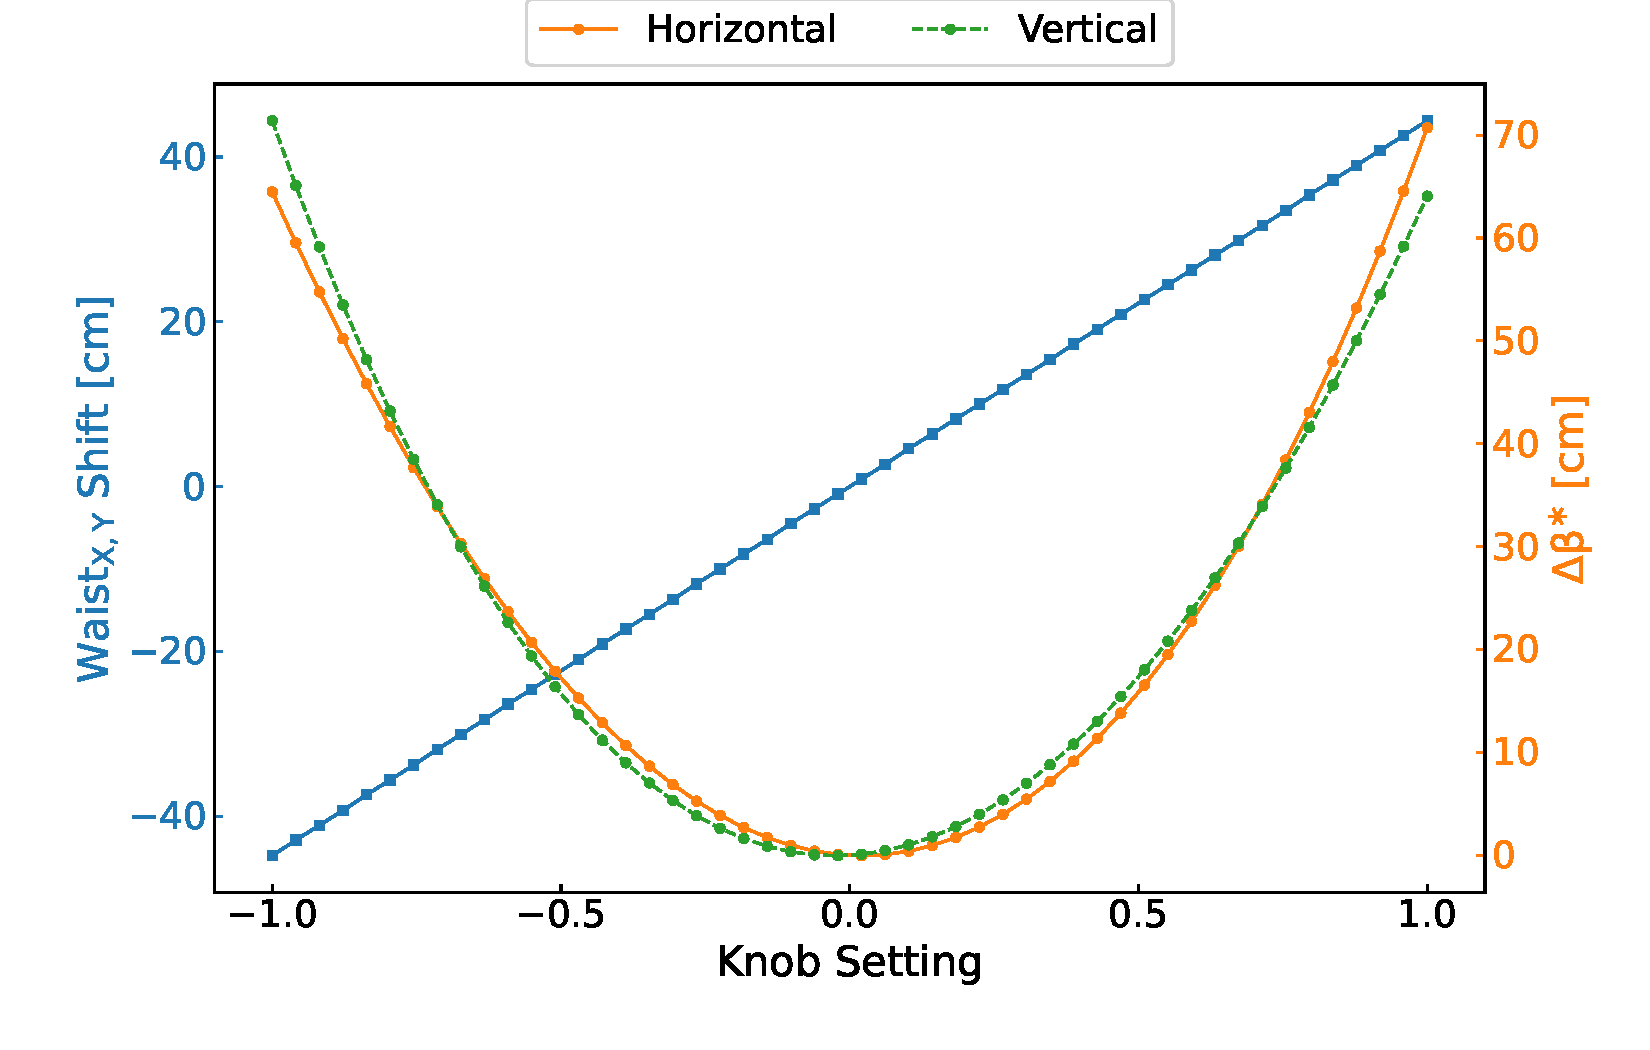
\includegraphics[width=\textwidth]{Figures/IR_Coupling_Correction/rigid_waist_shift_waist_effect_combined.pdf}
    \caption{Simulated effect of the designed Rigid Waist Shift knob as defined in \cref{table:rigid_waist_shift_knob} on the \(\beta^{\ast} =\)~\qty{30}{\centi\metre} optics of \num{2022}. The \textcolor{mplblue}{blue} line represents the waist displacement from the design location. The \textcolor{mplorange}{orange} and \textcolor{mplgreen}{green} lines represent the horizontal and vertical \(\beta\)-functions change at the IP as the waist is displaced, respectively.}
    \label{figure:rigid_waist_shift_knob_effect_on_waist}
\end{figure}

The waist displacement from the design location (\textcolor{mplblue}{blue} line) is almost completely linear with the knob setting.
One can note that the minima of the parabolas indicating the change of \(\beta\)-functions at the IP (\textcolor{mplblue}{blue} and \textcolor{mplorange}{orange} curves) are not found at exactly the zero knob setting, which is because the LHC design optics include a very small waist at IP\num{1} and IP\num{5}.

In \cref{figure:rigid_waist_shift_knob_effect_on_betas} one can observe how the \(\beta\)-functions are affected by the application of an RWS, also simulated with the \(\beta^{\ast} =\)~\qty{30}{\centi\metre} optics of \num{2022}.
In this simulation the lattice was sliced to improve the resolution of the data points, which explains the smoother lines compared to, for instance, \cref{figure:lhc_ir5_zoomed}.
One can observe how the (anti-)symmetry of the optics in the IR is broken when applying the knob (full vs dashed lines): the horizontal (\textcolor{mplb}{blue}) and vertical (\textcolor{mplr}{red}) \(\beta\)-functions do not mirror each other anymore.
Inset zooms are included around the location of the MQSX magnets (\textcolor{mqsx_green}{green} vertical lines), showing how the horizontal and vertical \(\beta\)-functions are modified in their vicinity.
The purpose of this setup is detailed in \cref{subsection:rws_application_and_simulations}.

\begin{figure}[!htb]
    \centering
    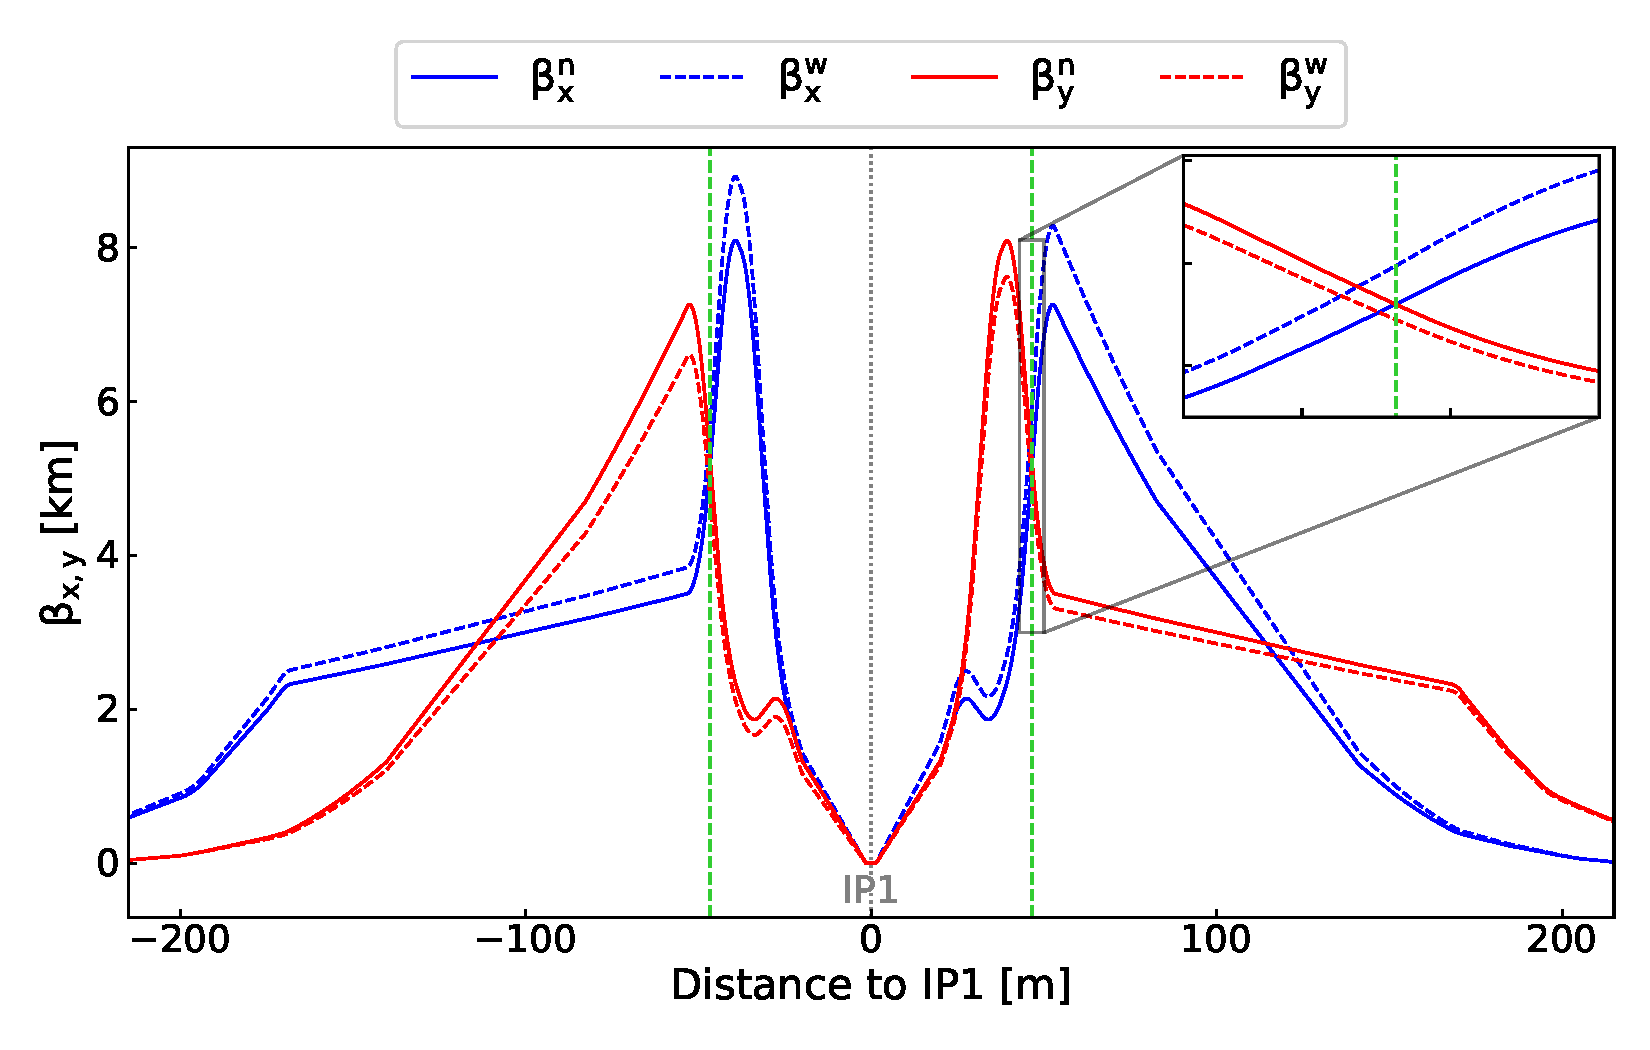
\includegraphics[width=\textwidth]{Figures/IR_Coupling_Correction/rigid_waist_shift_betas_effect.pdf}
    \caption{Simulated effect of the designed RWS knob on the \(\beta\)-functions around IP\num{1}, with the \(\beta^{\ast} =\)~\qty{30}{\centi\metre} optics of \num{2022}. The \(\beta\)-functions for both the horizontal (\textcolor{mplb}{blue}) and vertical (\textcolor{mplr}{red}) planes are shown for the nominal (full lines) and shifted waists (dashed lines) scenarios. An identical result is found for IP\num{5}.}
    \label{figure:rigid_waist_shift_knob_effect_on_betas}
\end{figure}

\subsubsection*{Optics Impact and Rematching}

Predictably, the application of a Rigid Waist Shift as described above has a strong impact on the optics across the machine.
This is due to the significant change of \(\beta\)-functions in the triplets, which sends a beating wave from the IR to the rest of the machine.
Applying an RWS with a unit setting of \num{1}, as defined in \cref{table:rigid_waist_shift_knob}, leads to a \numrange[range-phrase = --]{20}{30}\unit{\percent} increase in peak \gls{beta-beating} throughout the machine, depending on the observed beam and plane.

This can be observed in \cref{figure:rigid_waist_shift_betabeating}, where in simulations an RWS was implemented with a unit setting of \num{1} at IP\num{1} and the optics deviations from the nominal scenario were determined across the machine for both beams.
The most affected beam and plane depends on the setting of the RWS: in \cref{figure:rigid_waist_shift_betabeating} beam~\num{1} horizontal and beam~\num{2} vertical are most affected, but these would be beam~\num{1} vertical and beam~\num{2} horizontal if the RWS was applied with a setting of \num{-1}.
Naturally, some strong outliers can be observed in the vicinity of the IP, which correspond to the desired deviation at the IP and in the triplets induced by the \gls{knob} \gls{trim}.
\break

\begin{figure}[!htb]
    \centering
    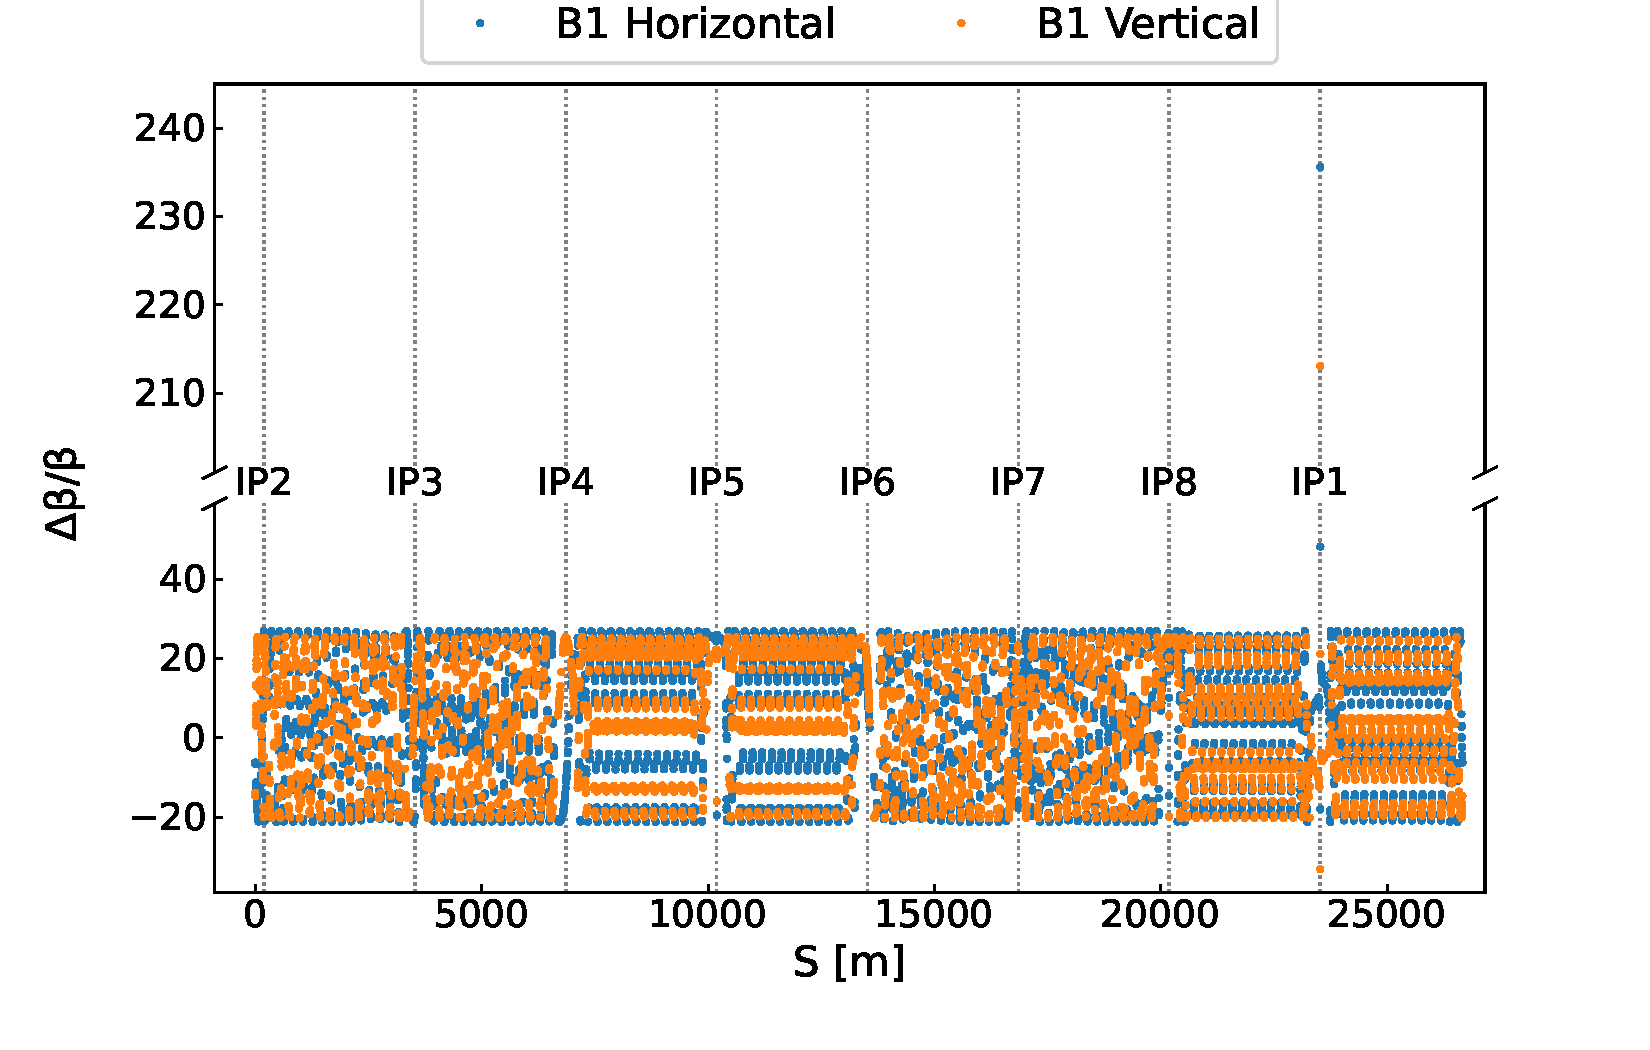
\includegraphics[width=\textwidth]{Figures/IR_Coupling_Correction/rws_ir1_b1_bbeating.pdf}
    \caption{Simulated \(\beta\)-beating induced across beam~\num{1} in both the horizontal (\textcolor{mplblue}{blue}) and vertical (\textcolor{mplorange}{orange}) planes, from applying an RWS as defined in \cref{table:rigid_waist_shift_knob} at IP\num{1}. A \numrange{20}{30}\unit{\percent} \(\beta\)-beating is observed through most of the machine, with (wanted) outliers close to IP\num{1}.}
    \label{figure:rigid_waist_shift_betabeating}
\end{figure}

Such a deviation of the optics has an impact on correction knobs.
For instance, simulations show that application of the RWS causes a \qty{15}{\percent} deviation from the achieved \glssymbol{Cminus} to the target value set through the LHC global coupling knobs, used for coupling correction with the arc skew quadrupoles.
Additionally, the optics deviations will change the impact of any errors probed while the RWS is trimmed in, namely the skew quadrupolar impact on the \gls{Cminus} (see \cref{equation:deltaqmin_guignard}).

In order to limit this impact on the optics and guarantee good measurements under an RWS, new correction knobs have been developed that make use of individually powered quadrupoles Q\num{4} to Q\num{10} (included). 
These knobs tune the optics functions and rematch them at the edges of the IR in the large sense.
They were designed with the \gls{MADX} code and a software developed for the occasion that can create these experimental configurations for a given IP in the machine~\cite{CODE:Soubelet:pyrws}.

These knobs are obtained from simulations after applying an RWS in a given IR and iterating several matching routines for quantities of interest at different locations in the machine.
Importantly, no involved magnet sees its powering change by more than \(\sim\)\qty{3}{\percent} with the application of these knobs, which allows for respecting the powering limits of individually powered elements.
As the rematching knobs depend on the RWS setting and optics configuration, many variations are possible and no general definition table is available akin to \cref{table:colinearity_knob,table:rigid_waist_shift_knob}.
A full definition of the rematching knobs for the \(\beta^{\ast} =\)~\qty{30}{\centi\meter} optics of 2022 as used in the LHC can be found in \cref{section:optics_rematching_knobs_lsa}.

\Cref{figure:rws_rematching_efficiency} shows a comparison of the simulated optics deviation in the beam~\num{1} horizontal plane, induced by the RWS before (\textcolor{mplblue}{blue}) and after (\textcolor{mplorange}{orange}) applying the rematching knob, here implemented at IP\num{1}.
Across the machine the \gls{beta-beating} is brought down by \(\sim\)\qty{20}{\percent} to around \(\sim\)\qty{5}{\percent} depending on the beam and plane compared to the nominal scenario, except for the vicinity of the IP where the desired deviation is kept unchanged.
A \qty{5}{\percent} \(\beta\)-beating across the machine is an acceptable level as it is similar to the level of control achieved during normal operation with all corrections trimmed in (see \cite{PRAB:Persson:LHC_Optics_Commissioning_OnePercent,CERN:Persson:LHCOpticsCorrectionsEvian2019}), as can be seen in \cref{figure:virgin_vs_corrected_lhcb2}.

While only beam~\num{1} horizontal is shown in this figure, results are similar for all planes of beam~\num{1} and beam~\num{2}.
As the rematching depends on the desired configuration (given optics and setting of the RWS) a knob has to be designed for each beam, at each IR and for each RWS setting.

\begin{figure}[!htb]
    \centering
    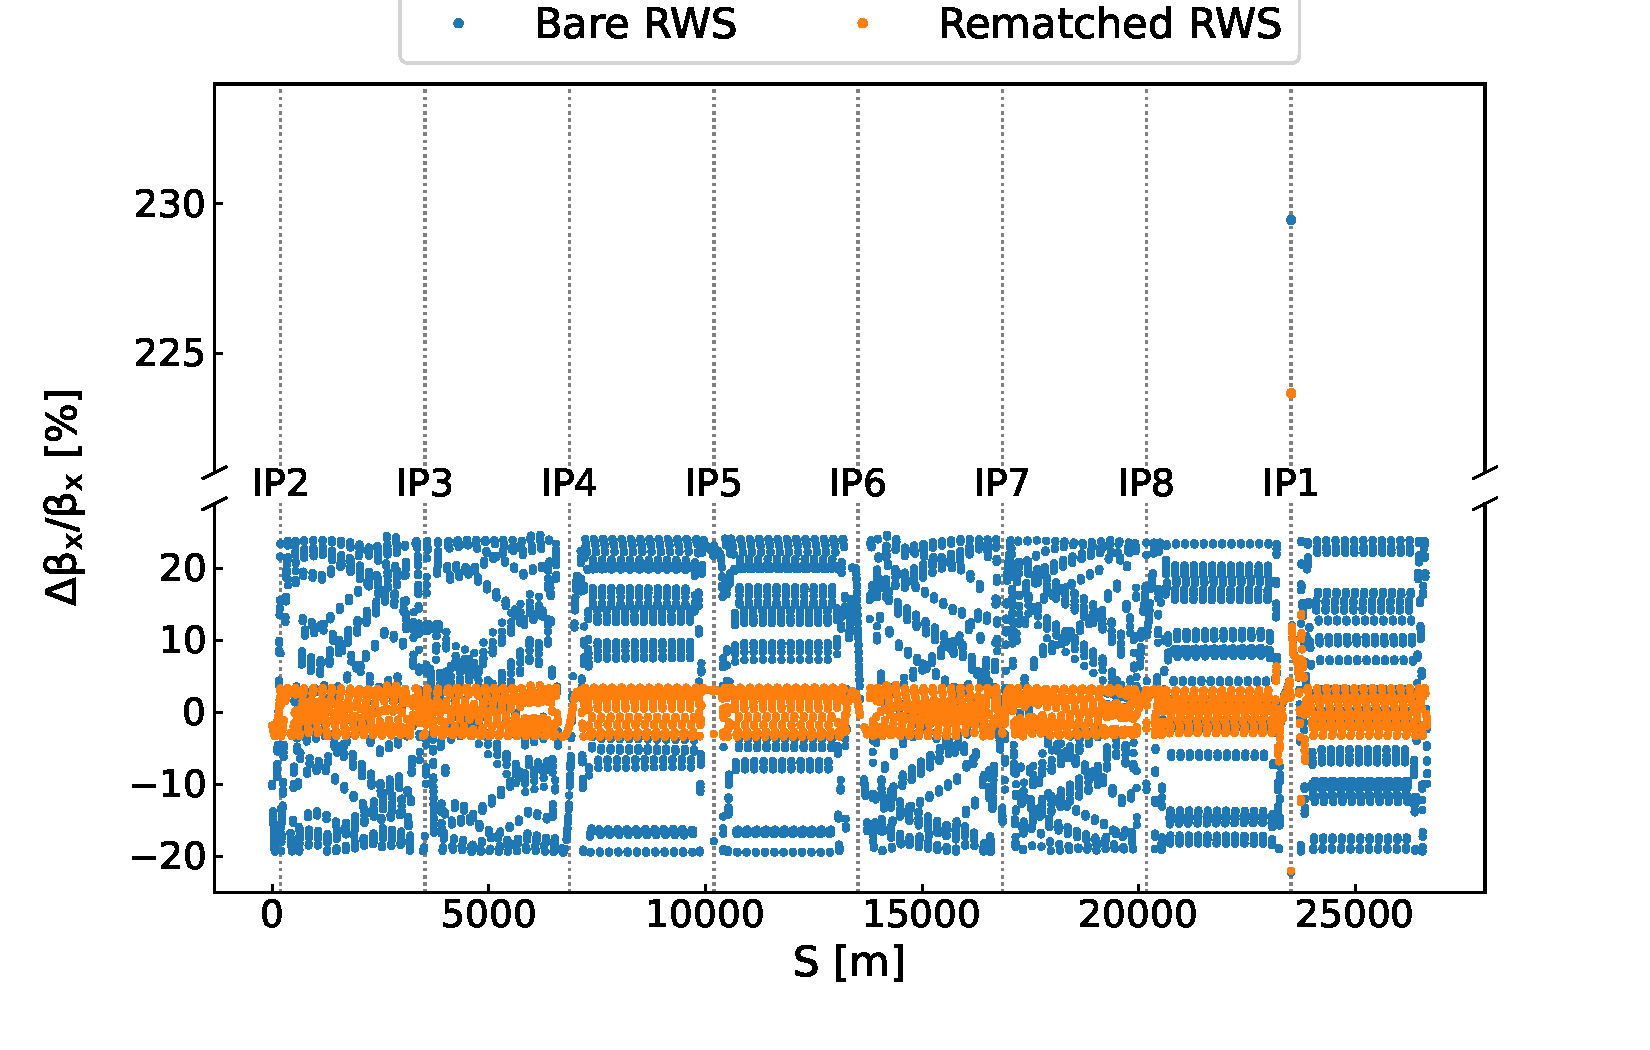
\includegraphics[width=\textwidth]{Figures/IR_Coupling_Correction/rws_ir1_b1_bbeating_rematched.pdf}
    \caption{Simulated \(\beta\)-beating induced across the machine in the beam~\num{1} horizontal plane from applying an RWS at IP\num{1}, before (\textcolor{mplblue}{blue}) and after (\textcolor{mplorange}{orange}) applying the optics rematching knob.}
    \label{figure:rws_rematching_efficiency}
\end{figure}

One can notice that near the IP the beating is also lowered by the rematching, but stays high enough to still break the symmetry of the IR.
\Cref{figure:rws_ir1_rematching_betas} shows the \(\beta\)-functions around IP\num{1} before (full lines) and after (dashed lines) application of the rematching knobs.
One can observe how the deviation between the two cases is negligible close to the IP and, importantly, in both cases the symmetry of the IR is broken compared to, for instance, \cref{figure:lhc_ir5_zoomed}.

\begin{figure}[!htb]
    \centering
    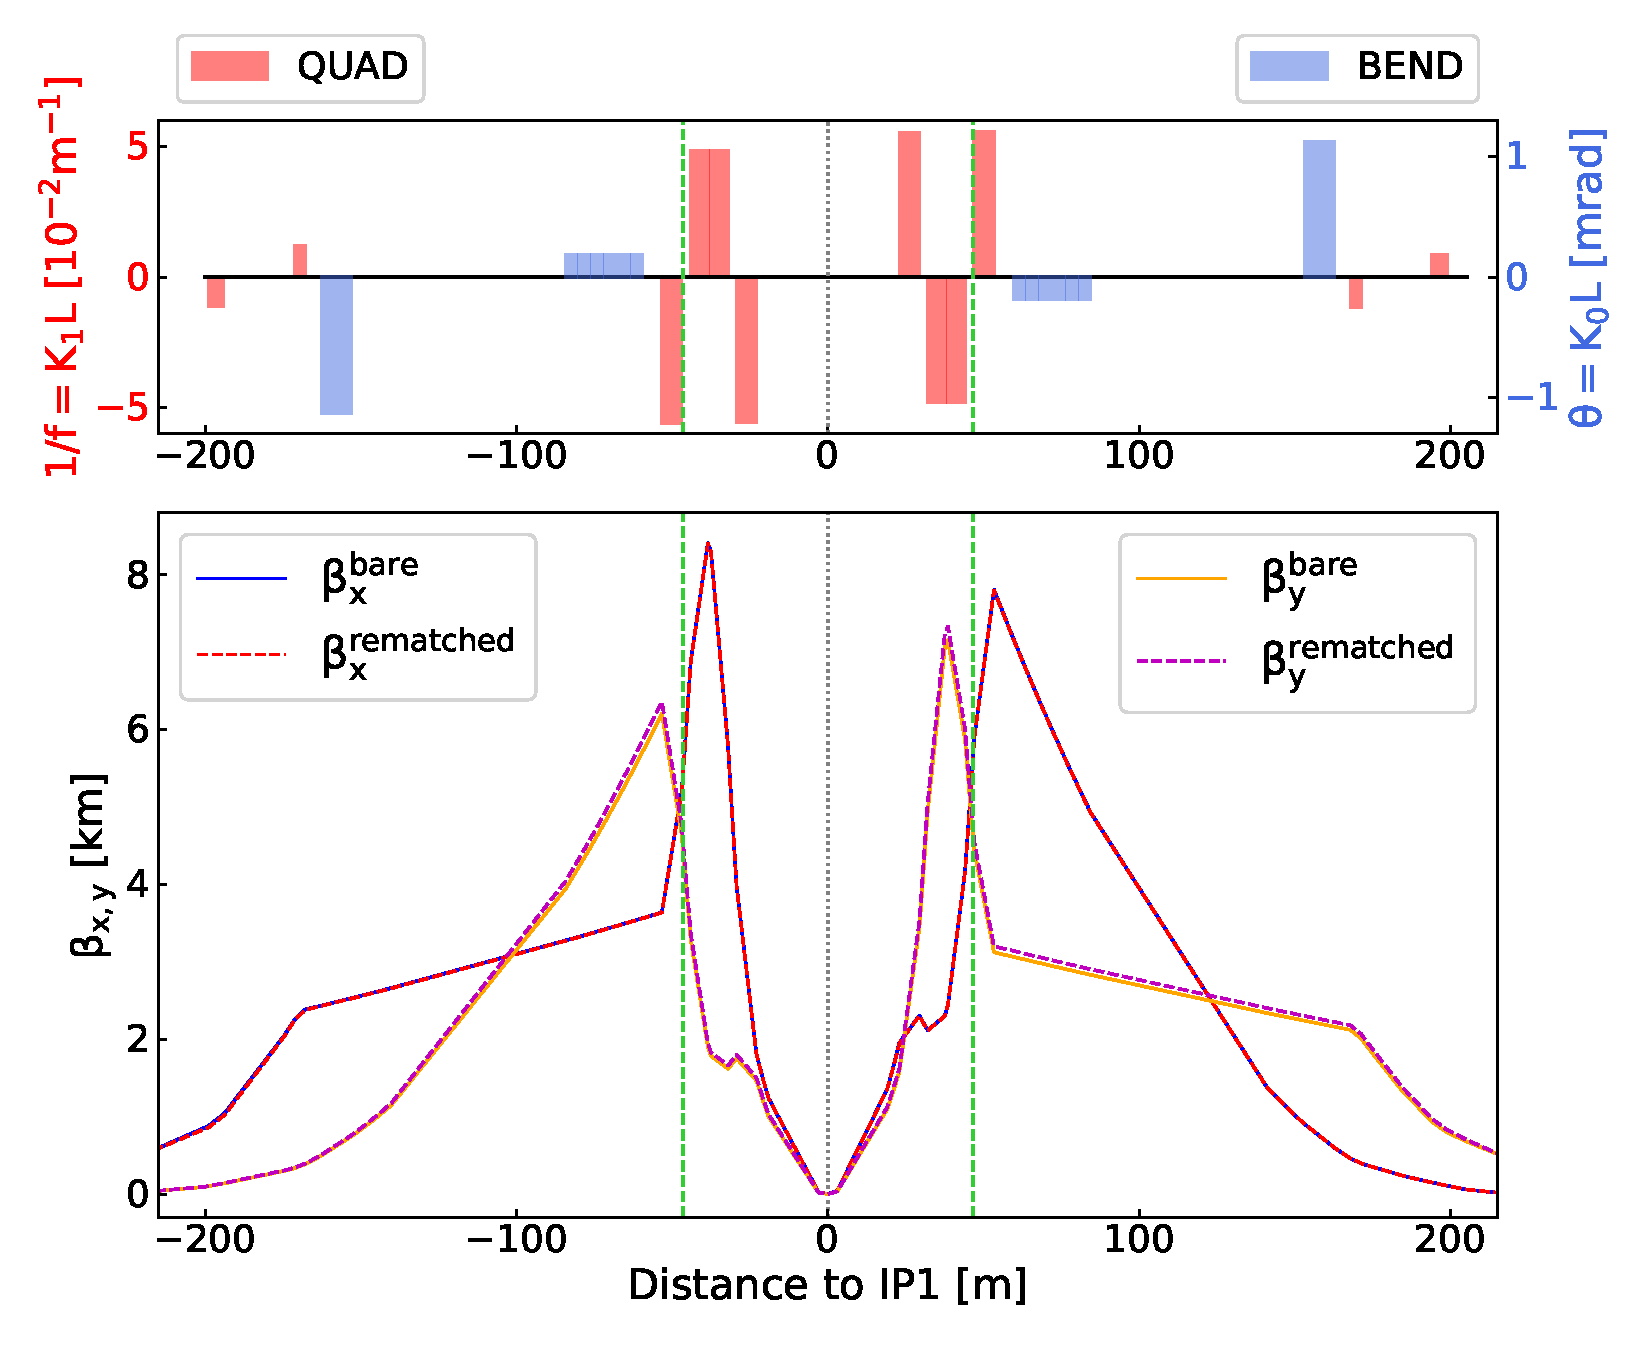
\includegraphics[width=\textwidth]{Figures/IR_Coupling_Correction/rws_ir1_rematching.pdf}
    \caption{Simulated \(\beta\)-functions around IP\num{1} when applying an RWS, before (full lines) and after (dashed lines) application of the rematching knobs, with the \(\beta^{\ast} =\)~\qty{30}{\centi\metre} optics of \num{2022}.}
    \label{figure:rws_ir1_rematching_betas}
\end{figure}

\subsection{Application Concept and Simulations}
\label{subsection:rws_application_and_simulations}

Making away with the optics symmetry of the \gls{IR} allows to break the locality of any coupling bump, even a truly local one.
As can be seen on the inset zooms of \cref{figure:rigid_waist_shift_knob_effect_on_betas}, with the application of an RWS the \(\beta\)-functions at the MQSX magnets change enough that the \(\sqrt{\beta_x \beta_y}\) term in \cref{equation:deltaqmin_only_mqsxs} are different at the two magnets.
\Cref{table:sqrt_betas_from_rws} shows the values of these terms with and without an RWS applied.
Phase advances are also changed, but by a very small amount.

\begin{table}[!htb]
    \centering
    \begin{tblr}{colspec={ccc}}
        \hline
        \SetCell[r=2,c=1]{m,c} \textbf{Magnet} & \SetCell[c=2]{c} \textbf{\(\sqrt{\beta_x \beta_y}\) [\unit{\square\meter}]}   \\
        \cline{2,3}                            &  Without an RWS            &    With an RWS                                   \\
        \hline
        MQSX.3L[IP]                            &    \num{5193.084265}       &     \num{5186.603944}                            \\
        MQSX.3R[IP]                            &    \num{5199.142377}       &     \num{5396.527580}                            \\
        \hline
    \end{tblr}
    \caption{Values of the \(\sqrt{\beta_x \beta_y}\) term in \cref{equation:deltaqmin_only_mqsxs} at the MQSX magnets around IP\num{1} or IP\num{5} without (left) and with (right) the application of an RWS, with the \(\beta^{\ast} =\)~\qty{30}{\centi\metre} optics of \num{2022}.}
    \label{table:sqrt_betas_from_rws}
\end{table}

\Cref{figure:rdt_leak} shows the coupling \glspl{RDT} from a closed coupling bump around the IP created through the colinearity knob, both in the presence (\textcolor{mplr}{red}) and absence (\textcolor{mplb}{blue}) of an RWS.

\begin{figure}[!htb]
    \centering
    \includegraphics*[width=\textwidth]{Figures/IR_Coupling_Correction/waist_shift_leaks_rdts.pdf}
    \caption{Amplitudes of the linear coupling RDTs in the vicinity of IP\num{1} under a coupling bump, with (\textcolor{mplr}{red}) and without (\textcolor{mplb}{blue}) an RWS. The vertical \textcolor{mqsx_green}{green} lines represent the positions of the skew quadrupoles correctors (MQSX.\num{3}[RL]\num{1}) used to implement the coupling bump. A colinearity knob setting of \num{10} and a rigidity waist shift knob setting of \num{1} were used.}
    \label{figure:rdt_leak}
\end{figure}
\break

When applying a Rigid Waist Shift and breaking the optics symmetry of the IR, one can observe a leakage of the coupling \glspl{RDT} outside the limits of the initial coupling bump.
These RDTs will then have a residual presence in the machine, which can be measured and reconstructed from turn-by-turn data from \glspl{BPM} with more suitable phase advances.
As a consequence, under an RWS even a local coupling bump that would normally be invisible to the rest of the machine will have a direct impact on the global coupling, measured as the \glssymbol{Cminus}.
This can be seen in \cref{figure:knob_to_cminus_with_waist}, where changes in the setting of the colinearity knob now have a strong effect on the \glssymbol{Cminus} when an RWS is applied in the relevant \gls{IR}.

\begin{figure}[!htb]
    \centering
    \includegraphics*[width=0.99\textwidth]{Figures/IR_Coupling_Correction/colin_knob_vs_waist_shift.pdf}
    \caption{Impact of the colinearity knob on the global \(\abs{C^{-}}\), calculated according to \cref{equation:deltaqmin_from_f1001}, with (\textcolor{mplblue}{blue}) and without (\textcolor{mplorange}{orange}) applying an RWS.}
    \label{figure:knob_to_cminus_with_waist}
\end{figure}

As previously mentioned, since the bump is not actually perfectly closed the \textcolor{mplorange}{orange} line in \cref{figure:knob_to_cminus_with_waist} is not completely flat and reaches up to \(\sim\)~\num{1e-5}, which is well below the measurement accuracy for the \(\abs{C^{-}}\).
The behavior seen in \cref{figure:knob_to_cminus_with_waist}, though theoretical, has been experimentally tested and confirmed in the machine~\cite{CERN:Persson:Local_Coupling_IP}.
Importantly, this behavior opens the possibility of using an RWS to probe IR local coupling through the measured global coupling.

Simulations have been done to investigate the feasibility of finding local coupling correction settings using an RWS, with the \(\beta^{\ast} = \) \qty{30}{cm} optics of \num{2022}.
At both IR\num{1} and IR\num{5} a local coupling bump was created by introducing identical tilt errors in triplet quadrupoles Q\num{3} - thus giving a skew quadrupolar component - and the colinearity knob was powered for compensation.
A full parameter space was explored, both with and without an RWS applied.
\Cref{figure:cminus_colin_vs_tilt_with_waist} shows the values of the resulting \(\abs{C^{-}}\) across the parameter space when an RWS is applied.
\Cref{figure:beam_size_colin_vs_tilt_no_waist} shows the resulting IP beam size increase as a ratio to the nominal beam size across the same parameter space.

\begin{figure}[!htb]
    \centering
    \includegraphics*[width=0.95\textwidth]{Figures/IR_Coupling_Correction/cminus_colin_tilt_compensation_with_waist.pdf}
    \caption{Resulting \(\abs{C^{-}}\) (\cref{equation:deltaqmin_from_f1001}) for various combinations of tilt error and colinearity knob settings, when applying an RWS.}
    \label{figure:cminus_colin_vs_tilt_with_waist}
\end{figure}

\begin{figure}[!htb]
    \centering
    \includegraphics*[width=0.95\textwidth]{Figures/IR_Coupling_Correction/ip_beam_size_growth_colin_tilt_compensation_no_waist.pdf}
    \caption{Resulting beam size (\cref{equation:lebedev_beam_size}) increase for identical settings of tilt error and colinearity knob settings as \cref{figure:cminus_colin_vs_tilt_with_waist}, but without an RWS.}
    \label{figure:beam_size_colin_vs_tilt_no_waist}
\end{figure}

The results of \cref{figure:beam_size_colin_vs_tilt_no_waist} highlight that minimization of the growth is possible, though a wrong setting would enhance the phenomenon.
A great correlation between beam size growth from the local coupling bump (without RWS, see \cref{figure:cminus_colin_vs_tilt_with_waist}) and the \glssymbol{Cminus} from leaked RDTs (with RWS, see \cref{figure:beam_size_colin_vs_tilt_no_waist}) is observed.

Simulations replicating a more complex scenario - akin to operational conditions - were also performed.
In these, tilt errors were introduced in triplet quadrupoles Q\num{3} as previously to create a closed local coupling bump around the IP.
Additionally, some tilt errors were added to an individually powered quadrupole in IR\num{5} (for instance Q\num{5}) to include the presence of expected residual local coupling errors in the other main IR, which contribute to the global coupling by the amount of \num{1e-3}.
Some global coupling sources were also added with a dedicated knob~\cite{CERN:Tomas:Optimizing_Global_Coupling_Knobs_LHC} that bring the global coupling to \num{1e-2}, which was then corrected through a routine and brought down to \(\sim\)\num{3e-3}, a level similar to what is achieved in the machine~\cite{PRES:Persson:Transverse_Coupling_OMC_OP,PRES:Persson:Transverse_Coupling_Stability_HLLHC_WP2}.
The RWS and colinearity knobs were then powered to different settings, and the resulting \glssymbol{Cminus} and IP beam sizes were determined in all settings combinations.

Similar to the previous studies made for \cref{figure:cminus_colin_vs_tilt_with_waist,figure:beam_size_colin_vs_tilt_no_waist}, an entire parameter space of implemented errors and corrections has been explored.
The evolution of both the \(\abs{C^{-}}\) and the beam size growth at IP\num{1} for one of these simulations can be seen in \cref{figure:full_scenario_colin_correction_dqmin_lebedev}.
These curves would correspond to a vertical line in \cref{figure:cminus_colin_vs_tilt_with_waist,figure:beam_size_colin_vs_tilt_no_waist}, but with a realistic scenario.

\begin{figure}[!htb]
    \centering
    \includegraphics*[width=\textwidth]{Figures/IR_Coupling_Correction/full_scenario_cminus_and_ip_size.pdf}
    \caption{Resulting \(\abs{C^{-}}\) under an RWS (\textcolor{mplorange}{orange}) and IP\num{1} beam size (\cref{equation:lebedev_beam_size}) without an RWS relative to the nominal scenario (\textcolor{mplblue}{blue}), for various colinearity knob settings. The black dotted line represents the threshold of a \qty{1}{\percent} beam size increase from the nominal scenario.}
    \label{figure:full_scenario_colin_correction_dqmin_lebedev}
\end{figure}

It can be observed that settings minimizing the measured \(\abs{C^{-}}\) under an RWS are very close to minimizing the coupling induced beam size increase without said RWS.
Here these settings also compensate for the contribution of the other added sources, on top of the local ones.
Similarly to previous studies a great correlation is observed, and across the parameter space one computes a \num{0.96} Pearson correlation coefficient between the quantities shown in \cref{figure:full_scenario_colin_correction_dqmin_lebedev}.
This confirms the link between the measured \(\abs{C^{-}}\) and the quantities of interest at the IP location.
To summarize:

\begin{itemize}
    \item Thanks to the RWS, sources leading to truly local coupling can be probed through their forced impact on global coupling.
    \item Using the correlation properties demonstrated above, one can find settings to minimize the coupling and its effects at the IP.
\end{itemize}

\subsection{Determining Corrections}

The corrections which would compensate only the local sources are determined by comparing the measured \(\abs{C^{-}}\) to simulations, such as the orange line in \cref{figure:full_scenario_colin_correction_dqmin_lebedev}.

In the real machine, some coupling will remain in the arcs due to a non-perfect global correction and non-local SbS corrections.
As the method probes local errors' impact through the \(\abs{C^{-}}\), it will naturally be sensitive to the global coupling in the machine, which should be replicated in simulations.
Although the overall behavior of simulations remains similar when including this component, an important change from the line seen in \cref{figure:full_scenario_colin_correction_dqmin_lebedev} is the location of the setting that minimizes the \(\abs{C^{-}}\).
The relevance of this property will be discussed below.
By comparing measurements from a colinearity knob scan to simulations - where the former includes the impact of local errors, but the latter does not - one can single out the contribution of the local sources to global coupling.
This is illustrated in \cref{figure:full_scenario_determine_correction}.

\begin{figure}[!htb]
    \centering
    \includegraphics*[width=0.95\textwidth]{Figures/IR_Coupling_Correction/full_scenario_determine_correction.pdf}
    \caption{Resulting \(\abs{C^{-}}\) in simulations as done for \cref{figure:full_scenario_colin_correction_dqmin_lebedev}, with (\textcolor{mplblue}{blue}) and without (\textcolor{mplorange}{orange}) local coupling sources in IR\num{1}.}
    \label{figure:full_scenario_determine_correction}
\end{figure}

\Cref{figure:full_scenario_determine_correction} shows the resulting \(\abs{C^{-}}\) values under an RWS during a colinearity knob scan, for one of the simulation scenarios mentioned previously (\cref{figure:full_scenario_colin_correction_dqmin_lebedev}) (\textcolor{mplblue}{blue}), and a similar scenario in which no local coupling sources were implemented in IR\num{1} (\textcolor{mplorange}{orange}).
The former represents what would be measured in the machine, including the contribution of local sources.
The latter represents a simulation to compare such a measurement to, which includes all contributions to global coupling except for the IR local sources.
The highlighted difference between the two curves is then fully explained by the local sources.

Applying a trim of the colinearity knob setting linearly translates the curves of \cref{figure:full_scenario_determine_correction} horizontally.
This behavior is valid and verifiable in both simulation and measurements.
Therefore, one looks to determine a colinearity knob trim that, if applied in the machine, would bring the measurement's \(\abs{C^{-}}\) minimization point to that of the simulation.
As this difference if fully explained by local sources, this trim contains the information on the local error in terms of colinearity knob setting: powering of the corrector magnets.
In \cref{figure:full_scenario_determine_correction} the minima are highlighted with vertical lines and the aforementioned correction trim is determined from the relative position of these two minima.
The value is different from that of the minimization in \cref{figure:full_scenario_colin_correction_dqmin_lebedev} as there global sources are also compensated while this correction aims at compensating only the local sources.

\begin{figure}[!htb]
    \centering
    \includegraphics*[width=0.95\textwidth]{Figures/IR_Coupling_Correction/full_scenario_correction_efficiency.pdf}
    \caption{Relative IP beam sizes when compared to the nominal scenario (\textcolor{mplblue}{blue}) when inputting the local errors used in the study for \cref{figure:full_scenario_determine_correction} (\textcolor{mplorange}{orange}) and after applying the suggested correction (\textcolor{mplgreen}{green}). The black dotted line represents the threshold of a \qty{1}{\percent} beam size increase from the nominal scenario.}
    \label{figure:full_scenario_correction_efficiency}
\end{figure}

When only considering the local sources used for the results in \cref{figure:full_scenario_determine_correction} and inputting the correction trim suggested, one obtains a good compensation of the beam sizes at IP\num{1}.
\Cref{figure:full_scenario_correction_efficiency} shows the impact of these local errors and the effect of applying the suggested correction trim.
The exactitude and effectiveness of the determined correction can be improved by performing more granular scans of the colinearity knob, but the values used are representative of what can be done in measurements.

\subsubsection*{Reproducing the Machine's Coupling}

The reproduction of the machine's global coupling in simulations becomes necessary as soon as strong non-IR sources are present, which is likely in the real machine.
Unfortunately the true distribution of sources in the machine is not known, and this reproduction can then be done in different ways.
In studies, various implementations were tested: random tilts in all quadrupoles, LHC specific knobs~\cite{CERN:Tomas:Optimizing_Global_Coupling_Knobs_LHC}, longitudinal misalignment of sextupoles, field errors in specific magnets or random combinations of the above.
The resulting \glssymbol{Cminus} for these can be seen in \cref{figure:global_coupling_modeling_impact}, where for each scenario the minimization point is highlighted by a vertical dashed line.

\begin{figure}[!hbt]
    \centering
    \includegraphics*[width=\textwidth]{Figures/IR_Coupling_Correction/global_sources_influence.pdf}
    \caption{Resulting simulated \(\abs{C^{-}}\) under an RWS during a scan of the colinearity knob, for various implementations of global coupling in the machine. For each case a vertical dashed line highlights the location of the minimization point.}
    \label{figure:global_coupling_modeling_impact}
\end{figure}

In all investigated scenarios the achieved \(\abs{C^{-}}\) before applying the RWS is the same value before (\(\sim 10^{-2}\)) and after (\(\sim 2 \cdot 10^{-3}\)) applying a correction routine.
It was found that, to the levels of coupling we achieve after correcting the machine the distribution and implementation of sources had little impact on the minimization point of the \(\abs{C^{-}}\) curve under an RWS, as long as the overall pattern of the \(f_{1001}\) and the level of coupling measured in the machine were accurately reproduced.

One can see in \cref{figure:global_coupling_modeling_impact} how the minimization point is relatively unchanged by the global coupling implementation method within the precision of the mesh step used for the scan, which was chosen to reflect that achievable in the machine.
As a consequence, in simulations this reproduction was done by including the coupling correction knobs implemented in the machine, as determined during earlier commissioning steps.

\subsection{Rigid Waist Shift Procedure}

To summarize so far, two tools have been developed and presented to tackle local coupling correction:
\begin{itemize}
    \item The colinearity knob (\cref{table:colinearity_knob}) allows adjusting the coupling at the \gls{IP} without affecting the rest of the machine, namely previously established corrections.
    \item The \acrlong{RWS} knob (\cref{table:rigid_waist_shift_knob}) allows probing local errors through the \glssymbol{Cminus} (\cref{figure:rdt_leak,figure:knob_to_cminus_with_waist}) and to find a correction setting of the colinearity knob that will minimize the coupling at the \gls{IP} (\cref{figure:full_scenario_determine_correction,figure:full_scenario_correction_efficiency}).
\end{itemize}

Using those, the complete correction procedure for local linear coupling is then made of three steps:
\begin{enumerate}
    \item Firstly, calculating and applying a correction of the IR contribution to global coupling based on RDTs from turn-by-turn measurements, using the SbS technique.
    \item Secondly, breaking the optics symmetry between the right and left-hand side of the IP by applying an RWS, and performing a scan of the colinearity knob.
    \item Finally, analyzing the measurements data and comparing it to simulations in order to find a colinearity knob adjustment setting that minimizes the global coupling, without impacting the correction found in step~\num{1}.
\end{enumerate}

These measurements can be performed for each IR and for each beam, and the subsequent determined corrections can then be directly applied in the machine.

\section{Local Coupling Correction in the LHC 2022 Commissioning}
\label{section:rws_experimental_results}

Below are presented experimental results of local coupling correction in the \acrshort{LHC}'s first year of \Gls{run}~\num{3}, during the \num{2022} commissioning, using the \gls{RWS} procedure presented above.
One can refer to \cref{appendix:experimental_knobs} for information on the fills used for experimental measurements.

\subsection{Segment-by-Segment Corrections}
\label{subsection:sbs_corrections}

In October \num{2021} a week of beam tests was done in the LHC at injection energy.
From the measurements at \qty{450}{\giga\electronvolt} a first set of local coupling corrections were calculated for each of the four main \glspl{IR} using the segment-by-segment technique.
\Cref{figure:beam_test_sbs_abs_f1001_ip5} shows the segment-by-segment results for the absolute value of the \(f_{1001}\) \gls{RDT} in IR\num{5}, from the \num{12}\({}^\mathrm{th}\) BPM left to right of IP\num{5}.
The vertical grey line indicates the location of the IP in the segment.
Due to the \gls{skew} quadrupole correctors in the IRs being single aperture magnets, one needs to find a single powering setting that works for both beams and both are shown on the figure.

\begin{figure}[!htb]
    \centering
    \includegraphics*[width=\textwidth]{Figures/IR_Coupling_Correction/beamtest_sbs_abs_f1001_ip5.pdf}
    \caption{Propagation of the measured \(\abs{f_{1001}}\) (\textcolor{mplblue}{blue}) around IP\num{5} (dashed grey line) and of the reconstructed values from the determined correction (\textcolor{mplorange}{orange}), measured at \qty{450}{\giga\electronvolt} and \(\beta^{*}=\) \qty{11}{\meter}.}
    \label{figure:beam_test_sbs_abs_f1001_ip5}
\end{figure}

One can see that the determined correction in IR\num{5} matches the propagated measurement within the tolerance of the error bars at the edges of the segment.
This guarantees a good compensation of the IR's contribution to global coupling.

During the LHC Run~\num{3} commissioning, local coupling corrections determined during the previous year's beam test were trimmed in the machine from the start.
After reaching the \(\beta^{*}=\) \qty{30}{\centi\meter} optics, where the machine is more sensitive to local errors, a noticeable deviation around IP\num{1} was observed and a refinement of the correction was determined, still with the segment-by-segment technique.
\Cref{figure:commissioning_sbs_real_f1001_ip1,,figure:commissioning_sbs_imag_f1001_ip1} show the effect of the new correction on the real and imaginary parts of the \(f_{1001}\) RDT in the segment, respectively.

\begin{figure}[!htb]
    \centering
    \includegraphics*[width=\textwidth]{Figures/IR_Coupling_Correction/commissioning_sbs_real_f1001_ip1.pdf}
    \caption{Propagation of the measured \(\Re f_{1001}\) (\textcolor{mplblue}{blue}) around IP\num{1} (dashed grey line) and the reconstructed values from the determined correction (\textcolor{mplorange}{orange}), measured at \qty{6.8}{\tera\electronvolt} and \(\beta^{*}=\) \qty{30}{\centi\meter}.}
    \label{figure:commissioning_sbs_real_f1001_ip1}
\end{figure}
  
\begin{figure}[!htb]
    \centering
    \includegraphics*[width=\textwidth]{Figures/IR_Coupling_Correction/commissioning_sbs_imag_f1001_ip1.pdf}
    \caption{Propagation of the measured \(\Im f_{1001}\) (\textcolor{mplblue}{blue}) around IP\num{1} (dashed grey line) and the reconstructed values from the determined correction (\textcolor{mplorange}{orange}), measured at \qty{6.8}{\tera\electronvolt} and \(\beta^{*}=\) \qty{30}{\centi\meter}.}
    \label{figure:commissioning_sbs_imag_f1001_ip1}
\end{figure}

The beating observed from the old correction was re-matched thanks to a setting adjustment where the IR\num{1} right-hand side corrector's powering was changed by \qty{1e-4}{\per\square\meter}.
The final correction settings determined with the segment-by-segment technique and trimmed in the machine at the four main \glspl{IR} can be found in \cref{table:sbs_corrections}, along with their counterpart values from \Gls{run}~\num{2} for comparison.

% \begin{table}[!htb]
%     \centering
%     \begin{tblr}{colspec={ccc}}
%         \hline
%         \SetCell[r=2,c=1]{c} \textbf{Circuit} & \SetCell[c=2]{c} \textbf{\(K_{1\mathrm{S}}\)~[\qty{1e-4}{\per\square\meter}]}              \\
%         \cline{2,3}
%                                  &    \textbf{2016-2018}~\cite{CERN:Persson:LHCOpticsCorrectionsEvian2019}    &    \textbf{2022 SbS}  \\
%         \hline
%             \textbf{RQXS.3L1}    &    \num{11}                                                                &     \num{8}           \\
%             \textbf{RQXS.3R1}    &    \num{7}                                                                 &     \num{7}           \\
%             \hline[dashed]
%             \textbf{RQXS.3L2}    &    \num{-14}                                                               &     \num{-14}         \\
%             \textbf{RQXS.3R2}    &    \num{-14}                                                               &     \num{-14}         \\
%             \hline[dashed]
%             \textbf{RQXS.3L5}    &    \num{7}                                                                 &     \num{6}           \\
%             \textbf{RQXS.3R5}    &    \num{7}                                                                 &     \num{6}           \\
%             \hline[dashed]
%             \textbf{RQXS.3L8}    &    \num{-5}                                                                &     \num{-5}          \\
%             \textbf{RQXS.3R8}    &    \num{-5}                                                                &     \num{-5}          \\
%         \hline
%     \end{tblr}
%     \caption{Local IR skew quadrupole correctors powering at the four main LHC IRs as determined with the segment-by-segment technique in the \num{2022} commissioning (right) and their values as used during the LHC Run~\num{2} (left).}
%     \label{table:sbs_corrections}
% \end{table}

\begin{table}[!htb]
    \centering
    \begin{tblr}{colspec={cccc}}
        \hline
        \SetCell[r=2,c=1]{c} \textbf{IR}  &  \SetCell[r=2,c=1]{c} \textbf{Circuit} & \SetCell[c=2]{c} \textbf{\(K_{1\mathrm{S}}\)~[\qty{1e-4}{\per\square\meter}]}                    \\
        \cline{3,4}
                                          &                                        &  \textbf{2016-2018}~\cite{CERN:Persson:LHCOpticsCorrectionsEvian2019}    &    \textbf{2022 SbS}  \\
        \hline
        \SetCell[r=2,c=1]{c} \textbf{IR1} &  \textbf{RQXS.3L1}                     &  \num{11}                                                                &     \num{8}           \\
                                          &  \textbf{RQXS.3R1}                     &  \num{7}                                                                 &     \num{7}           \\
        \hline[dashed]
        \SetCell[r=2,c=1]{c} \textbf{IR2} &  \textbf{RQXS.3L2}                     &  \num{-14}                                                               &     \num{-14}         \\
                                          &  \textbf{RQXS.3R2}                     &  \num{-14}                                                               &     \num{-14}         \\
        \hline[dashed]
        \SetCell[r=2,c=1]{c} \textbf{IR5} &  \textbf{RQXS.3L5}                     &  \num{7}                                                                 &     \num{6}           \\
                                          &  \textbf{RQXS.3R5}                     &  \num{7}                                                                 &     \num{6}           \\
        \hline[dashed]
        \SetCell[r=2,c=1]{c} \textbf{IR8} &  \textbf{RQXS.3L8}                     &  \num{-5}                                                                &     \num{-5}          \\
                                          &  \textbf{RQXS.3R8}                     &  \num{-5}                                                                &     \num{-5}          \\
        \hline
    \end{tblr}
    \caption{Local IR skew quadrupole correctors powering at the four main LHC IRs as determined with the segment-by-segment technique in the \num{2022} commissioning and their values as used during the LHC Run~\num{2}.}
    \label{table:sbs_corrections}
\end{table}

\subsection{Rigid Waist Shift Corrections}
\label{subsection:rws_pos_measurements_corrections}

The RWS method was implemented in both IR\num{1} and IR\num{5} at \qty{6.8}{\tera\electronvolt} and \(\beta^{*}=\) \qty{30}{\centi\meter} to determine final correction settings in the form of adjustments from the SbS corrections presented above.
Relevant fills used for these measurements can be found in \cref{table:run3_fills}.
\break

As a first step, the validity of the experimental setup was verified by trimming the RWS in the machine and then checking the efficiency of the optics rematching knobs.
\Cref{figure:ir5_rws_rematching} shows the \gls{beta-beating} across the machine for beam~\num{1} before any knob application (\textcolor{butter}{yellow}), from applying the RWS in IR\num{5} (\textcolor{skyblue}{blue}) and after the application of the optics re-matching knob (\textcolor{scarletred}{red}).
Similar checks were done for both beams and both IRs.
The \glspl{beta-function} in these measurements are reconstructed with the \acrshort{OMC} codes according to~\cite{PRAB:Wegscheider:Analytical_N_BPM}.

The measured impact is in agreement with what was expected from earlier simulations (see \cref{subsection:rigid_waist_shift}), leading to a \num{15}-\qty{25}{\percent} additional \(\beta\)-beating in the machine depending on the observed beam and plane; while the re-matching knob brought this beating back to about \qty{5}{\percent} where it was previously kept thanks to existing corrections.
Considering the state of the machine at the time of these measurements, it can be considered that the optics re-matching shows great efficiency.
Naturally, some strong deviations are noticed close to IP\num{5} (going out of range of the y-axis) as the optics there are changed on purpose, but also because \(\beta\)-functions reconstruction close the IPs is of relatively low quality.

After confirming the validity of the optics knobs and with the waist shift in the machine, scans of the colinearity knob (\cref{table:colinearity_knob}) were performed.
At each setting, a few measurements were taken by method of beam excitation, from which the coupling \glspl{RDT} were computed.
As the \gls{optics} are affected - and re-matched - differently for beam~\num{1} and beam~\num{2}, a scan of the colinearity knob was performed for each beam and for each IR.
Different scans were done with different granularity due to time constraints.

\begin{figure}[!htb]
    \centering
    \includegraphics*[width=\textwidth]{Figures/IR_Coupling_Correction/rematching_knob_efficiency.pdf}
    \caption{The beam~\num{1} \(\beta\)-beating observed at \qty{6.8}{\tera\electronvolt} and \(\beta^{*}=\)~\qty{30}{\centi\meter} for the corrected machine (\textcolor{butter}{yellow}), from the implementation of the RWS in IR\num{5} (\textcolor{skyblue}{blue}) and after applying the optics re-matching knob (\textcolor{scarletred}{red}). The highlighted area (\textcolor{highlightorange}{orange}) shows where magnetic elements are affected by the knobs.}
    \label{figure:ir5_rws_rematching}
\end{figure}

For each measurement the RDTs across the machine are normalized to the base case with no RWS, global coupling corrected and no colinearity knob trim.
Only then is the \glssymbol{Cminus} computed according to \cref{equation:deltaqmin_from_f1001}.
Then the variations due to the changes of the colinearity knob are visualized and compared to simulations.
In said simulations, the global coupling of the machine is reproduced by introducing the coupling correction knobs implemented in the machine at the time of measurements.

In \cref{figure:ir1_b1_pos_measurement,figure:ir1_b2_pos_measurement,figure:ir5_b1_pos_measurement,figure:ir5_b2_pos_measurement} comparisons are shown between simulations and scan measurements at IR\num{1} for beam~\num{1} and beam~\num{2}, then IR\num{5} for beam~\num{1} and beam~\num{2}, respectively.
The delta between minimization settings, corresponding to the suggested correction adjustment, is highlighted on each plot.
The relatively low range of achieved \glssymbol{Cminus} values is due to the aforementioned \glspl{RDT} normalization.
The noticeably different behavior of beam~\num{1} and beam~\num{2} simulations is explained by the different coupling situation in each beam: throughout commissioning beam~\num{2} has showcased little global coupling to be corrected while beam~\num{1} required significantly stronger global coupling corrections, as well as local adjustments for different arcs.
As these are reproduced in simulations, this difference of behavior is unsurprising.

\begin{figure}[!htb]
    \centering
    \includegraphics*[width=0.94\textwidth]{Figures/IR_Coupling_Correction/rws_measurement_ir1_b1_pos.pdf}
    \caption{Measurement scan done at IR\num{1} for beam \num{1} (\textcolor{mplr}{red}) and simulations for the same setup (\textcolor{mplblue}{blue}). The minima of both curves are highlighted by vertical dashed lines and the delta between the two, suggesting the remaining error to correct, is displayed on the graph.}
    \label{figure:ir1_b1_pos_measurement}
\end{figure}

\begin{figure}[!htb]
    \centering
    \includegraphics*[width=0.94\textwidth]{Figures/IR_Coupling_Correction/rws_measurement_ir1_b2_pos.pdf}
    \caption{Measurement scan done at IR\num{1} for beam \num{2} (\textcolor{mplr}{red}) and simulations for the same setup (\textcolor{mplblue}{blue}). The minima of both curves are highlighted by vertical dashed lines and the delta between the two, suggesting the remaining error to correct, is displayed on the graph.}
    \label{figure:ir1_b2_pos_measurement}
\end{figure}

\begin{figure}[!htb]
    \centering
    \includegraphics*[width=0.94\textwidth]{Figures/IR_Coupling_Correction/rws_measurement_ir5_b1_pos.pdf}
    \caption{Measurement scan done at IR\num{5} for beam \num{1} (\textcolor{mplr}{red}) and simulations for the same setup (\textcolor{mplblue}{blue}). The minima of both curves are highlighted by vertical dashed lines and the delta between the two, suggesting the remaining error to correct, is displayed on the graph.}
    \label{figure:ir5_b1_pos_measurement}
\end{figure}

\begin{figure}[!htb]
    \centering
    \includegraphics*[width=0.94\textwidth]{Figures/IR_Coupling_Correction/rws_measurement_ir5_b2_pos.pdf}
    \caption{Measurement scan done at IR\num{5} for beam \num{2} (\textcolor{mplr}{red}) and simulations for the same setup (\textcolor{mplblue}{blue}). The minima of both curves are highlighted by vertical dashed lines and the delta between the two, suggesting the remaining error to correct, is displayed on the graph.}
    \label{figure:ir5_b2_pos_measurement}
\end{figure}

In \cref{figure:ir1_b1_pos_measurement,figure:ir1_b2_pos_measurement,figure:ir5_b1_pos_measurement,figure:ir5_b2_pos_measurement}, simulations for beam~\num{2} suggest that the (small) reproduced global coupling has little effect on the procedure, and the colinearity knob scan could almost be used alone to determine the corrections.
For beam~\num{1} simulations however the impact of the reproduced global coupling appears much more substantial, as was the case in the machine, and this highlights the need to compare the scan measurements to simulations.
Overall, this comparison is needed in the case that there are significant coupling errors in the arcs.
It is worth noting that both beams' measurements converge to similar correction suggestions.
\break

\Cref{table:rws_corrections_summary} shows a summary of the suggested correction settings for each beam and IR.
While slightly different corrections are suggested from independent scans of beam~\num{1} and beam~\num{2}, it is possible that both values are simultaneously true.
Indeed, while most of the error contribution is expected to come from the dual-beam triplet quadrupoles and be common to both beams, errors in double aperture magnets Q\num{4} to Q\num{10} would affect each beam individually and force a divergence of the suggested correction adjustments for each beam.\\

\begin{table}[!htb]
    \centering
    $\begin{tblr}{colspec={ccc}}
        \hline
        \SetCell[r=2,c=1]{m,c} \textbf{Scan} & \SetCell[c=2]{c} \textbf{Suggested \( \Delta k \)~[\(10^{-4}\)\unit{\meter^{-2}}]} \\
        \cline{2,3}
                                             &  \textbf{Beam~\num{1}}  &  \textbf{Beam~\num{2}}     \\
        \hline
        \textbf{IR1}                         &  \num{-3.5}             &  \num{-3}                   \\
        \hline[dashed]
        \textbf{IR5}                         &  \num{-2}               &  \num{-1.5}                 \\
        \hline
    \end{tblr}$
    \caption{Correction adjustments suggested from the Rigid Waist Shift scans analysis, on top of the existing segment-by-segment corrections that were in the machine (see \cref{table:sbs_corrections}).}
    \label{table:rws_corrections_summary}
\end{table}

Furthermore, the orbit and hence feed-down but also the \(\beta\) ratio between sources and correctors are different for both beams, which could explain part of the difference.
As the main contributors to the error are the triplets, it is not unsurprising to obtain similar correction suggestions for both beams.

Some more measurements were performed with an opposite setting of the \gls{RWS} in both \glspl{IR} that did not yield sensible correction suggestions, which have not been shown here.
For completeness, these are exposed in \cref{appendix:inconclusive_measurements} together with the suspected reasons for each one's failure.

\subsection{Luminosity Confirmation}
\label{subsection:lumi_correction_trims}

Later on during the \num{2022} physics run, beam time was allocated to trim in the suggested adjustments from \cref{table:rws_corrections_summary}.
The impact of the corrections was assessed based on instantaneous luminosity measurements at the time of the trims.
Time was found to perform measurements of the efficiency of corrections in each IR at both \(\beta^{\ast} =\)~\qty{30}{\centi\meter} and \(\beta^{\ast} =\)~\qty{42}{\centi\meter}.
Information on the fills used can be found in \cref{table:md_fills}.

For each measurement, trims around the suggested correction adjustments were also performed in order to look for the best local setting, which might not necessarily have been found by the method.
Below are shown data from the trims at \(\beta^{\ast} =\)~\qty{30}{\centi\meter} only, while \(\beta^{\ast} =\)~\qty{42}{\centi\meter} results are compiled in a later table.

\Cref{figure:corrections_trims_ir1} shows the trim performed at IR\num{1} (\textcolor{mplblue}{blue}) and subsequent measured luminosity changes at the \acrshort{ATLAS} experiment (\textcolor{mplorange}{orange}).
The light blue area highlights the trim values suggested by the RWS method, which vary for beam~\num{1} and beam~\num{2}.
The instantaneous luminosity signal slightly trails up after the end of the correction adjustment trim as the ATLAS experiment publishes a time-averaged value.
A great improvement in luminosity can be observed from the trim, with an almost \qty{10}{\percent} improvement from the adjustment.

\begin{figure}[!htb]
    \centering
    \includegraphics*[width=\textwidth]{Figures/IR_Coupling_Correction/corrections_trim_ir1.pdf}
    \caption{Trim of the colinearity knob setting (\textcolor{mplblue}{blue}) and observed IP\num{1} instantaneous luminosity change (\textcolor{mplorange}{orange}) at \qty{6.8}{\tera\electronvolt} and \(\beta^{\ast} = \) \qty{30}{cm}. The blue area highlights the trim values suggested by the RWS method, which varies for beam~\num{1} and beam~\num{2}.}
    \label{figure:corrections_trims_ir1}
\end{figure}

\Cref{figure:corrections_trims_ir5} shows the trim performed at IR\num{5} during the same fill.
Once again the trim of the colinearity knob is shown in \textcolor{mplblue}{blue} and the recorded luminosity change at the \acrshort{CMS} experiment in \textcolor{mplorange}{orange}.
Similarly to \cref{figure:corrections_trims_ir1}, the light blue area highlights the trim values suggested by the RWS method.
The luminosity data outliers observed in the plot are either luminosity measurement artifacts or changes from adjustment to the head-on scheme and can be safely dismissed, as they are located outside the time periods of the trims.

Unfortunately, due to higher priority tasks for the operators at the time, the trim was not completed in a single go to the target value and as a result the luminosity decreased in the time between the different parts of the trim.
\Cref{figure:corrections_trims_ir5_zoomed} shows a cut view of the data, where the downtime in between the various parts of the trim has been left out (notice the cut in the horizontal axis).
The overall improvement from the complete trim is estimated from the individual observed luminosity improvements of the different parts of the trim, and amount to an almost \qty{4}{\percent} increase from the adjustment.

\begin{figure}[!htb]
    \centering
    \includegraphics*[width=0.94\textwidth]{Figures/IR_Coupling_Correction/corrections_trim_ir5.pdf}
    \caption{Trim of the colinearity knob setting (\textcolor{mplblue}{blue}) and observed IP\num{5} instantaneous luminosity change (\textcolor{mplorange}{orange}) at \qty{6.8}{\tera\electronvolt} and \(\beta^{\ast} = \) \qty{30}{cm}. The blue area highlights the trim values suggested by the RWS method, which varies for beam~\num{1} and beam~\num{2}.}
    \label{figure:corrections_trims_ir5}
\end{figure}

\begin{figure}[!htb]
    \centering
    \includegraphics*[width=0.94\textwidth]{Figures/IR_Coupling_Correction/corrections_trim_ir5_split.pdf}
    \caption{Zoomed view of the colinearity knob setting (\textcolor{mplblue}{blue}) and observed IP\num{5} instantaneous luminosity change (\textcolor{mplorange}{orange}) at \qty{6.8}{\tera\electronvolt} and \(\beta^{\ast} = \) \qty{30}{cm}. The blue area highlights the trim values suggested by the RWS method, which varies for beam~\num{1} and beam~\num{2}.}
    \label{figure:corrections_trims_ir5_zoomed}
\end{figure}

\Cref{table:rws_lumi_gains} gives a summary of the observed luminosity improvements for each performed trim, at both \(\beta^{\ast} =\)~\qty{30}{\centi\meter} and \(\beta^{\ast} =\)~\qty{42}{\centi\meter}.
Overall great improvements are obtained throughout, with the largest gains recorded for IP\num{1}.
It is expected to observe lower gains at a higher \(\beta^{\ast}\) since the \(\sqrt{\beta_x \beta_y}\) term of \cref{equation:deltaqmin_guignard_singular} is substantially lower in the triplets for the less squeezed optics, resulting in a smaller effect of any tilt error.
It is also expected to notice a lower improvement at the CMS detector based on the numbers in \cref{table:rws_corrections_summary}: a lower suggested adjustment indicates a smaller coupling error remains in IR\num{5} than in IR\num{1} after segment-by-segment corrections, and the subsequent smaller applied correction recovers less luminosity.\\

\begin{table}[!htb]
    \centering
    \begin{tblr}{colspec={ccc}}
        \hline
        \SetCell[r=2,c=1]{m,c} \textbf{Experiment} & \SetCell[c=2]{c} \textbf{Luminosity Gain [\unit{\percent}]}                    \\
        \cline{2,3}                                &    \(\beta^{\ast} = \) \qty{30}{cm}    &    \(\beta^{\ast} = \) \qty{42}{cm}   \\
        \hline
        \textbf{ATLAS (IP1)}                       &    \num{9.7}                           &    \num{5.2}                          \\
        \textbf{CMS (IP1)}                         &    \num{3.5}                           &    \num{1.5}                          \\
        \hline
    \end{tblr}
    \caption{Instantaneous luminosity gains observed at the main experiments ATLAS and CMS from the method's suggested corrections.}
    \label{table:rws_lumi_gains}
\end{table}

The adjustments determined with the RWS have been incorporated into the nominal corrector settings and the \gls{LHC} now uses the resulting \gls{skew} quadrupole powerings in normal operation.
\Cref{table:run2_vs_sbs_run3_vs_rws_run3_corrections} gives a summary of the final settings at the two main LHC IRs as well as a comparison to their values in previous years, as an update of \cref{table:sbs_corrections}.\\

% \begin{table}[!htb]
%     \centering
%     \begin{tblr}{colspec={cccc}}
%         \hline
%         \SetCell[r=2,c=1]{m,c} \textbf{Circuit} & \SetCell[c=3]{c} \textbf{\( K_{1\mathrm{S}} \)~[\(10^{-4}\)\unit{\meter^{-2}}]} \\
%         \cline{2,3,4}
%                                                 &    \textbf{2016-2018}~\cite{CERN:Persson:LHCOpticsCorrectionsEvian2019}    &    \textbf{2022 SbS}    &    \textbf{2022 RWS}  \\
%         \hline
%         \textbf{RQXS.3L1}                       &    \num{11}                                                                &     \num{8}             &     \num{11.5}        \\
%         \textbf{RQXS.3R1}                       &    \num{7}                                                                 &     \num{7}             &     \num{3.5}         \\
%         \hline[dashed]
%         \textbf{RQXS.3L5}                       &    \num{7}                                                                 &     \num{6}             &     \num{8}           \\
%         \textbf{RQXS.3R5}                       &    \num{7}                                                                 &     \num{6}             &     \num{4}           \\
%         \hline
%     \end{tblr}
%     \caption{Final values of corrections determined with segment-by-segment, compared to the values used in Run~\num{2} and the values after RWS adjustments for both IR\num{1} and IR\num{5}.}
%     \label{table:run2_vs_sbs_run3_vs_rws_run3_corrections}
% \end{table}

\begin{table}[!htb]
    \centering
    \begin{tblr}{colspec={ccccc}}
        \hline
        \SetCell[r=2,c=1]{c} \textbf{IR}  &  \SetCell[r=2,c=1]{c} \textbf{Circuit} & \SetCell[c=3]{c} \textbf{\(K_{1\mathrm{S}}\)~[\qty{1e-4}{\per\square\meter}]}                                              \\
        \cline{3,4,5}
                                          &                                        &  \textbf{2016-2018}~\cite{CERN:Persson:LHCOpticsCorrectionsEvian2019}    &    \textbf{2022 SbS}    &    \textbf{2022 RWS}  \\
        \hline
        \SetCell[r=2,c=1]{c} \textbf{IR1} &  \textbf{RQXS.3L1}                     &  \num{11}                                                                &     \num{8}             &     \num{11.5}        \\
                                          &  \textbf{RQXS.3R1}                     &  \num{7}                                                                 &     \num{7}             &     \num{3.5}         \\
        \hline[dashed]
        \SetCell[r=2,c=1]{c} \textbf{IR5} &  \textbf{RQXS.3L5}                     &  \num{7}                                                                 &     \num{6}             &     \num{8}           \\
                                          &  \textbf{RQXS.3R5}                     &  \num{7}                                                                 &     \num{6}             &     \num{4}           \\
        \hline[dashed]
    \end{tblr}
    \caption{Final values of local IR skew quadrupole correctors powering at the two main LHC experiments, as determined with segment-by-segment (middle), compared to the values used in the LHC Run~\num{2} (left) and the values after RWS adjustments (right).}
    \label{table:run2_vs_sbs_run3_vs_rws_run3_corrections}
\end{table}

\subsection{Comparison to Expectations}
\label{subsection:lumi_vs_expectations}

Simulations were performed to compare the observed luminosity improvements to what one would expect from correcting the suspected local errors.
As the adjustments were determined in terms of unit setting of the colinearity knob, one can consider these an accurate representation of the error that was left - and corrected - in the machine.
For instance, a correction of \(\Delta_{\mathrm{colin}} = 5\) suggests that the corrected local error in the machine could be reproduced by introducing a \num{-5} trim of the colinearity knob in simulations.

In these simulations, done at \qty{6.8}{\tera\electronvolt} using the \num{2022} optics, the nominal machine setup was reproduced and the suspected errors at either IR\num{1} or IR\num{5} were introduced in the form of a powering of the colinearity knob with the opposite values as those from \cref{table:rws_corrections_summary}.
Beam sizes were determined (\cref{equation:lebedev_beam_size}) for both beams in each case: with the trim of the colinearity knob, corresponding to the errored case; and without any trim, corresponding to the corrected case.
From these, instantaneous luminosities were determined according to \cref{equation:luminosity_double_beams}.
\Cref{figure:expected_vs_observed_lumigains} shows the expected values from simulations as well as the measured values as reported in \cref{table:rws_lumi_gains}.

\begin{figure}[!htb]
    \centering
    \includegraphics*[width=\textwidth]{Figures/IR_Coupling_Correction/expected_vs_observed_lumigains.pdf}
    \caption{The expected (lines) and observed (triangular markers) instantaneous luminosity changes at \qty{6.8}{\tera\electronvolt} for the various optics in the LHC cycle, for IP\num{1} (\textcolor{mplblue}{blue}) and IP\num{5} (\textcolor{mplorange}{orange}). Vertical dashed lines indicate the \(\beta^{\ast} =\)~\qty{30}{\centi\meter} and \(\beta^{\ast} =\)~\qty{42}{\centi\meter} data points.}
    \label{figure:expected_vs_observed_lumigains}
\end{figure}

While the expected luminosity gains at IP\num{5} are in agreement with the observed ones, some discrepancies are present for IP\num{1} data and a factor \(\sim\)\num{1.26} between the measurement and prediction is present.

\begin{warningblock}
    As will be seen later on in \cref{section:limited_correctors_availability}, similar measurements show a much better agreement with IP1 simulation predictions using the same calculations as in \cref{figure:expected_vs_observed_lumigains}. 
    Those measurements were taken later on in the year, with higher intensity beams - thus a higher quality of the \gls{luminosity} signal - and better detector setup and calibration.
    This leads us to believe the IP\num{1} luminosity measurement in \cref{figure:expected_vs_observed_lumigains} is an underestimation of the actual values.
    The expected value for the IR\num{1} trim, from measurements presented in \cref{section:limited_correctors_availability}, would be an \qty{11.6}{\percent} luminosity increase at \(\beta^{\ast} =\)~\qty{30}{\centi\meter}.
\end{warningblock}

\section{Relevance to Other Colliders}

For any collider the requirement of small \glspl{beta-function} for collisions is a key design parameter, and leads to using a doublet or triplet of quadrupoles to achieve the necessary intense focusing of the beams at the IP.
On either side of the collision point, in the drift space leading to the first quadrupole the \(\beta\)-functions evolve as:

\begin{equation}
    % \beta(s) = \beta^{\ast} + \frac{s^2}{\beta^{\ast}} \text{ .}
    \beta(s) = \beta^{\ast} + s^2 / \beta^{\ast} \text{ .}
    \label{equation:collider_drift_space_beta_function}
\end{equation}
where \glssymbol{betastar} is the \(\beta\)-function at the \gls{IP} and \(s\) denotes the distance from the IP.
Using \(L^*\) as the length of this drift space, the phase advance from the IP to said quadrupole is expressed as:

\begin{equation}
    \mu = \int_0^{L^*} \frac{1}{\beta(s)} ds = \int_0^{L^*} \frac{\beta^{\ast}}{\beta^{\ast}{}^2 + s^2} ds \text{ ,}
    \label{equation:collider_drift_space_phase_advance_integral}
\end{equation}
\vspace{1pt}

\noindent
which one can integrate to obtain:

\begin{equation}
    \mu = \beta^{\ast} \left[\frac{1}{\beta^{\ast}} \tan^{-1} \left(\frac{s}{\beta^{\ast}} \right) \right]_0^{L^*} = \tan^{-1} \left(\frac{L^*}{\beta^{\ast}} \right) \text{ .}
    \label{equation:collider_drift_space_phase_advance_integrated}
\end{equation}
\vspace{1pt}

Then, for traditionally \(L^* \gg \beta^{\ast}\) one gets:

\begin{equation}
    \mu \simeq \tan^{-1} \left( \infty \right) \simeq \frac{\pi}{2} \text{ .}
    \label{equation:collider_drift_space_phase_advance_approximation}
\end{equation}

As a consequence, for a typical collider layout the phase advance from left to right doublet / triplet quadrupoles is \(\sim \pi\).
This can be seen in \cref{figure:fccee_phases_to_ip5} for the \acrshort{FCC}-ee~\cite{EPJST:Abada:FCCee_Lepton_Collider} V\num{22} lattice for the Z operation mode, which uses an asymmetric doublet of quadrupoles.

\begin{figure}[!htb]
    \centering
    \includegraphics*[width=0.89\textwidth]{Figures/IR_Coupling_Correction/fccee_phases_to_ip5.pdf}
    \caption{Phase advances relative to IP\num{5} at in the FCC-ee V22 lattice, in the Z operation mode at \qty{45.6}{\giga\electronvolt} and \(\beta^{\ast}=\)~\qty{10}{\centi\meter}.}
    \label{figure:fccee_phases_to_ip5}
\end{figure}

As a further direct consequence, tilts in said quadrupoles are susceptible to create a coupling bump around the IP.
This can be seen, again for the FCC-ee V\num{22} lattice, in \cref{figure:fccee_ip5_coupling_bump}.

\begin{figure}[!htb]
    \centering
    \includegraphics*[width=\textwidth]{Figures/IR_Coupling_Correction/fccee_ip5_coupling_bump.pdf}
    \caption{Simulated amplitude of coupling RDTs \(f_{1001}\) (\textcolor{mplblue}{blue}) and \(f_{1010}\) (\textcolor{mplorange}{orange}) from a \qty{1}{\milli\radian} tilt in the first Q\num{1} quadrupoles around the FCC-ee's IP\num{5}.}
    \label{figure:fccee_ip5_coupling_bump}
\end{figure}

Furthermore, the segment-by-segment limitations encountered in the \gls{LHC} would also be present: no observation point is present at the \gls{IP}, and due to the large \(\beta\)-functions in the doublet quadrupoles the phase advance from element to element close to the IP is very close to \num{0}, making the accurate reconstruction of coupling \glspl{RDT} difficult (see \cref{subsection:reconstruction_linear_coupling_rdts}).

These conditions were confirmed in existing and future machines.
The \gls{HL-LHC} and FCC-hh lattices being based on the LHC's, they share the same limitations that have been exposed in this chapter.
The FCC-ee V\num{22} lattice, as shown above, also exhibits these conditions and could suffer from a close coupling bump from doublet tilts.
Another existing collider, SuperKEKB, has also encountered non-trivial issues with local coupling in their High Energy Ring~\cite{ICFA:Morita:Optics_Corrections_including_IP_Local_Coupling_at_SuperKEKB}.

As such, for the aforementioned accelerators but also more generally for most circular collider layouts, the presented use of a \acrlong{RWS} could provide a useful method to tackle local linear coupling.

\section{Operation with Limited Correctors Availability}
\label{section:limited_correctors_availability}

Magnets lifetime studies done during the \gls{longshutdown}~\num{2} (LS\num{2}) have projected that some magnets in the main \glspl{IR} will reach their radiation dose limit during \Gls{run}~\num{3}~\cite{PRES:Cerutti:TripletLifetime_Evian}, including the MQSX magnets used for local coupling correction.
\Cref{table:correctors_peak_dose}, reproduced from data presented in~\cite{PRES:Cerutti:TripletLifetime_Evian}, shows the expected total received dose for the skew quadrupole corrector magnets in the main IRs, for various scenarios.
% In \textcolor{red}{red} are highlighted the values exceeding design dose limits.

% \begin{table}[!htb]
%     \centering
%     \begin{tblr}{colspec={ccc}}
%         \hline
%         \SetCell[r=3,c=1]{m,c} \textbf{Magnets}    &    \SetCell[c=2]{c} \textbf{Peak Dose [\unit{\mega\gray}]}                                                                                    \\
%         \cline{2,3}                                &    With ATLAS Variable (Fixed) Angle                        &    +\num{2025} (as \num{2023}/\num{2024})                                       \\
%         \cline{2,3}                                &    After \qty{395}{\femto\barn^{-1}}                        &    After \qty{480}{\femto\barn^{-1}}                                            \\
%         \hline
%         \textcolor{red}{\textbf{MCBX1 (IR1)}}      &    \textcolor{red}{\num{8.5} (\num{8.5})}                   &    \textcolor{red}{\num{11} (\num{11}) $/$ \asterisk \num{10.5} (\num{10.5})}   \\
%         \textcolor{red}{\textbf{MCBX1 (IR5)}}      &    \num{6}                                                  &    \textcolor{red}{\num{7.5}}                                                   \\
%         \textbf{MCBX2 (IR1)}                       &    \num{3.5} (\num{3.5})                                    &    \num{4} (\num{4}) $/$ \asterisk \num{4} (\num{4})                            \\
%         \textbf{MCBX2 (IR5)}                       &    \num{2}                                                  &    \num{2.5}                                                                    \\
%         \textcolor{red}{\textbf{MQSX (IR1)}}       &    \textcolor{red}{\num{7.5} (\num{7.5})}                   &    \textcolor{red}{\num{9} (\num{9}) $/$ \asterisk \num{9} (\num{9})}           \\
%         \textcolor{red}{\textbf{MQSX (IR5)}}       &    \textcolor{red}{\num{8} (\num{8})}                       &    \textcolor{red}{\num{9.5} (\num{9.5})}                                       \\
%         \textbf{MCBX3 (IR1)}                       &    \num{5} (\num{5})                                        &    \num{6} (\num{6.5}) $/$ \asterisk \num{6} (\num{6})                          \\
%         \textbf{MCBX3 (IR5)}                       &    \num{3}                                                  &    \num{3.5}                                                                    \\
%         \hline
%     \end{tblr}
%     \caption{Expected total received dose of the corrector magnets located in the triplets for the main IRs. Table reproduced from~\cite{PRES:Cerutti:TripletLifetime_Evian}. The entries marked with \asterisk assume an IR\num{1} polarity inversion in the middle of \num{2025}.}
%     \label{table:correctors_peak_dose}
% \end{table}

\begin{table}[!hbt]
    \centering
    \begin{tblr}{colspec={ccc}}
        \hline
        \SetCell[r=2,c=1]{c} \textbf{Magnets}     &  \SetCell[c=2]{c} \textbf{Peak Dose [\unit{\mega\gray}]}                                                                                     \\
        \cline{2,3}                               &  After \qty{395}{\femto\barn^{-1}}  &  After \qty{480}{\femto\barn^{-1}}                     \\
        \hline
        % \textcolor{red}{MCBX\num{1} (IR\num{1})}  &  \textcolor{red}{\num{8.5}}       &  \textcolor{red}{\num{11} $/$ \asterisk \num{10.5}}    \\
        % \textcolor{red}{MCBX\num{1} (IR\num{5})}  &  \num{6}                          &  \textcolor{red}{\num{7.5}}                            \\
        % MCBX\num{2} (IR\num{1})                   &  \num{3.5}                        &  \num{4} $/$ \asterisk \num{4}                         \\
        % MCBX\num{2} (IR\num{5})                   &  \num{2}                          &  \num{2.5}                                             \\
        % \textcolor{red}{MQSX (IR\num{1})}         &  \textcolor{red}{\num{7.5}}       &  \textcolor{red}{\num{9} $/$ \asterisk \num{9}}        \\
        MQSX (IR\num{1})                            &  \num{7.5}                        &  \num{9}                                               \\
        % \textcolor{red}{MQSX (IR\num{5})}         &  \textcolor{red}{\num{8}}         &  \textcolor{red}{\num{9.5}}                            \\
        MQSX (IR\num{5})                            &  \num{8}                          &  \num{9.5}                                             \\
        % MCBX\num{3} (IR\num{1})                   &  \num{5}                          &  \num{6} $/$ \asterisk \num{6}                         \\
        % MCBX\num{3} (IR\num{5})                   &  \num{3}                          &  \num{3.5}                                             \\
        \hline
    \end{tblr}
    \caption{Expected total received dose of the MQSX magnets in the main IRs in Run~\num{3}. Table reproduced based on data from~\cite{PRES:Cerutti:TripletLifetime_Evian}.}
    \label{table:correctors_peak_dose}
\end{table}

One can notice that the MQSXs at both IR\num{1} and IR\num{5} are expected to surpass their dose limit of \qty{7}{\mega\gray} during Run~\num{3}.
The study itself highlights:

\begin{quoteblock}
    [\dots] assuming a limit of \qty{6}{\mega\gray} for the corrector magnets in the triplet, this is expected to be reached in the four MCBX.\num{1} and four MQSX by the end of 2024.
\end{quoteblock}

It is then warranted to prepare for one or more failures at some point during \Gls{run}~\num{3}, which would drastically impact the LHC's operations, potentially shutting the machine down depending on the severity of the failures.
It was therefore necessary to investigate the operational impact of losing one or more MQSX magnets in the main IRs, specifically in terms of machine safety and luminosity production.
For this, different failure scenarios and containment options were investigated that would try and compensate for one or more missing corrector.
The MQSX magnets in IR\num{2} and IR\num{8}, though not considered at risk, were still included in some of these studies.

\subsection{Operating with a Missing Corrector}

Should an MQSX stop functioning the priority is to ensure safe machine operation.
In the first place the impact of a single corrector failure around one of the main experiments was investigated.

\subsubsection*{Correction Load Carry Over}

As seen in \cref{section:colinearity_knob}, the contribution of one magnet can be replicated by its counterpart with a similar powering setting.
For instance, looking at \cref{table:run2_vs_sbs_run3_vs_rws_run3_corrections}, if the MQSX.\num{3}R\num{5} were to fail the loss of contribution to global coupling would be that of an MQSX magnet with  \(\mathrm{K_{1S}} =\)~\qty{-4E-4}{\per\square\meter} at this location.
It could be compensated by modifying the powering setting of MQSX.\num{3}L\num{5} by \qty{4E-4}{\per\square\meter}, since the optics conditions at the correctors are identical.
This compensation corresponds to a trim of \num{-4} units of the colinearity knob around IP\num{5} (see \cref{table:colinearity_knob}).

As such, should one MQSX fail it would still be possible to compensate for the \gls{IR}'s contribution to global coupling by properly powering its counterpart.
It would therefore be possible to fulfill the first correction stage mentioned in \cref{section:current_correction_methods_and_their_limitations} and to squeeze the beams down to \(\beta^{\ast} =\)~\qty{30}{\centi\meter}.
Minimizing coupling at the IP, however, would not be possible anymore as it requires trimming both magnets simultaneously.
The operational impact of losing one of the correctors would then be that of a potentially strong coupling at the IP.

Simulations were done with the \gls{MADX} code to assess the impact of missing a specific corrector magnet and compensating its effect by carrying its correction setting over to its counterpart on the other side of the IP.
In these simulations the powering settings from \cref{table:run2_vs_sbs_run3_vs_rws_run3_corrections} were used, as determined with the \gls{RWS}, and beam size increases were determined from Ripken parameters according to \cref{equation:lebedev_beam_size}.
From these, the changes in instantaneous luminosity were calculated according to \cref{equation:luminosity_double_beams}.

\Cref{figure:lumi_vs_trims_vs_betastars} shows the expected instantaneous luminosity reduction from the nominal case for various trims of the colinearity knob corresponding to different missing MQSX magnets, for different \(\beta^{\ast}\) optics.

\begin{figure}[!htb]
    \centering
    \includegraphics*[width=\textwidth]{Figures/IR_Coupling_Correction/lumi_vs_betastars_colin_trims.pdf}
    \caption{Expected instantaneous luminosity reduction for various trims of the colinearity knob at IP\num{1}/IP\num{5} for different \(\beta^{\ast}\) optics. Each line corresponds to the trim necessary to compensate for a specific corrector's powering.}
    \label{figure:lumi_vs_trims_vs_betastars}
\end{figure}

Should the most powered correctors fail, the instantaneous luminosity at the affected IP is expected to drop considerably at \(\beta^{\ast} =\)~\qty{30}{\centi\meter}: by up to \qty{60}{\percent}.
Importantly, as the powering limit of the MQSXs is \(\mathrm{K_{1S}} =\) \qty{30E-4}{\per\square\meter}, it would be possible to compensate for any failing one.
\newpage

The possible impact of this change on the aperture was also considered.
\Cref{figure:carry_over_impact_on_beam_size} shows the relative change in beam size around IP\num{1} with the \(\beta^{\ast} =\)~\qty{30}{\centi\meter} optics of \num{2023}, from the most important trim: carrying over the correction of the MQSX left of IP\num{1} to the MQSX right of IP\num{1}.

\begin{figure}[!htb]
    \centering
    \includegraphics*[width=\textwidth]{Figures/IR_Coupling_Correction/carry_over_to_ir1_right_beam_size_impact.pdf}
    \caption{Relative change in horizontal (\textcolor{mplblue}{blue}) and vertical (\textcolor{mplorange}{orange}) beam sizes from carrying over the correction of the MQSX left of IP\num{1} to the MQSX right of IP\num{1}.}
    \label{figure:carry_over_impact_on_beam_size}
\end{figure}

The beam sizes in the affected case are kept very close to the nominal ones at less than a \qty{1}{\percent} deviation through the machine, being significantly affected only in the space between the left to right Q\num{1} quadrupoles.
This behavior was also observed in~\cite{PRAB:Hofer:Coupling_Local_Observables} where the coupling \glspl{RDT} themselves are only significantly affected in the same space for a similar trim.
\Cref{figure:lhc_ir1_30cm_apertures} shows the physical aperture limitations of elements around IP\num{1} for the \(\beta^{\ast} =\)~\qty{30}{\centi\meter} optics, as well as representations of the beam envelopes at the same locations.

\begin{figure}[!htb]
    \centering
    \includegraphics*[width=\textwidth]{Figures/IR_Coupling_Correction/lhc_ir1_30cm_apertures.pdf}
    \caption{Magnets powering (top) and horizontal (middle) and vertical (bottom) aperture limitations around IP\num{1}, at \(\beta^{\ast} =\)~\qty{30}{\centi\meter}. The \textcolor{mplb}{blue} and \textcolor{mplr}{red} shaded areas represent, in each plane, the \(3 \sigma\), \(6 \sigma\) and \(11 \sigma\) beam envelopes, from darkest to lightest respectively. The grey blocks represent the physical locations of various elements.}
    \label{figure:lhc_ir1_30cm_apertures}
\end{figure}

As can be seen in \cref{figure:lhc_ir1_30cm_apertures} the triplet elements constitute the aperture bottleneck at \(\beta^{\ast} =\)~\qty{30}{\centi\meter}, while the drift space right around the IP is not a constraint for aperture limitations.
One can then conclude that the aperture would not suffer from such a compensation scheme.
Similarly, the impact on Beam-Beam Long Range (BBLR)~\cite{PHD:Poyet} interaction should be minimal as the increase is only significant within a meter of the \gls{IP} location itself.

\subsubsection*{Experimental Measurements of Carry-Over}

Measurements were conducted in late \num{2022} to assess the accuracy of these predictions.
A comparison of instantaneous luminosity loss from carrying over the left corrector's powering to the right one at IR\num{1} is shown in \cref{figure:ir1_carry_over_vs_simulation}, measured at \(\beta^{\ast} =\)~\qty{30}{\centi\meter}.
Carrying over the correction to the left magnet was not done due to time constraints.

\begin{figure}[!htb]
    \centering
    \includegraphics*[width=\textwidth]{Figures/IR_Coupling_Correction/ir1_scan_vs_simu.pdf}
    \caption{Instantaneous luminosity drop from correction carry-over to the right MQSX at IR\num{1} at \(\beta^{\ast} =\)~\qty{30}{\centi\meter}. The vertical grey line indicates the nominal operating point after the RWS correction adjustments.}
    \label{figure:ir1_carry_over_vs_simulation}
\end{figure}
\break

In \cref{figure:ir1_carry_over_vs_simulation}, the horizontal axis indicates the colinearity knob deviation from the baseline powering of the correctors determined with the segment-by-segment technique (see \cref{table:sbs_corrections}).
The vertical grey line indicates the nominal operating point after incorporating the \gls{RWS} correction adjustments (see \cref{table:rws_corrections_summary,table:run2_vs_sbs_run3_vs_rws_run3_corrections}), as well as the starting point of the scan.
This means the data point at \num{-0.5} on the horizontal axis (fourth from left) corresponds to a \(\Delta_{\mathrm{colin}} = 3\) \gls{trim} from the normal operating point, and similarly the data point at \num{8} on the horizontal axis corresponds to a \(\Delta_{\mathrm{colin}} = 11.5\) trim, which is the full carry-over of the correction from left to right MQSX.

\begin{noteblock}
    These are the IP\num{1} measurements mentioned in \cref{subsection:lumi_vs_expectations}.
    As one can see on \cref{figure:ir1_carry_over_vs_simulation}, the luminosity change from a \num{-3.5} units trim of the colinearity knob (from \num{0} to \num{-3.5} on the horizontal axis) shows a good agreement with expectations and leads to an \qty{11.6}{\percent} increase in the instantaneous luminosity.
    It is the same trim as performed earlier in the year, which can be seen in \cref{figure:corrections_trims_ir1}.
    This time however, the luminosity change is higher than the \qty{9.7}{\percent} initially measured, and closer to the \qty{12.25}{\percent} expected in \cref{figure:expected_vs_observed_lumigains}.
    As this measurement was performed with higher beam intensity and a better detector calibration it is more trusted.
\end{noteblock}

\Cref{figure:ir5_carry_over_vs_simulations} shows a similar comparison for IR\num{5}, also at \(\beta^{\ast} =\)~\qty{30}{\centi\meter}.
There again the nominal operating point corresponds to the \gls{RWS} adjustment from the SbS corrections and is indicated by the vertical grey line.
Due to time constraints again, however, the trim could not be fully done when carrying over the correction to the right corrector (\textcolor{mplorange}{orange} line).

\begin{figure}[!htb]
    \centering
    \includegraphics*[width=\textwidth]{Figures/IR_Coupling_Correction/ir5_scans_vs_simu.pdf}
    \caption{Instantaneous luminosity drop from correction carry-overs in both directions at IR\num{5} at \(\beta^{\ast} =\)~\qty{30}{\centi\meter}. The vertical grey line indicates the nominal operating point after the RWS correction adjustments.}
    \label{figure:ir5_carry_over_vs_simulations}
\end{figure}

In both \cref{figure:ir1_carry_over_vs_simulation,figure:ir5_carry_over_vs_simulations} simulations and measurements show a reasonable agreement.
Simulations systematically slightly over-estimate the loss of luminosity, particularly the larger the \gls{trim} is, but some discrepancy is to be expected as \cref{equation:luminosity_double_beams} is a simplified calculation.

\subsubsection*{Impact Through the Operational Cycle}

In Run~\num{3} a \(\beta^{\ast}\)-levelling was introduced in the LHC operational cycle to limit pile-up at the main IPs~\cite{MEETING:Fartoukh:Run3_Configuration}, as mentioned in \cref{section:lhc_operational_cycle}.
As seen in \cref{figure:lumi_vs_trims_vs_betastars} the luminosity losses depend on the \(\beta^{\ast}\), thus in order to keep operating at the pile-up limit one would have to take more frequent steps in the levelling, reducing its overall length as well as the integrated luminosity over the fill.

For instance, the levelling time would be reduced from \qty{8.2}{\hour} to \qty{1.23}{\hour} in the worst case, in which the MQSX.\num{3}L\num{1} were to fail.
Studies were done to assess the impact of operating with a single MQSX on the integrated luminosity over a fill, with \num{2023} settings.
The resulting integrated luminosity loss over a day is shown in \cref{figure:integrated_lumi_losses}, for each missing MQSX and for two different baselines of instantaneous luminosity~\cite{MEETING:Kostoglou:Integrated_Lumi_MQSX_Carryovers}.

\begin{figure}[!htb]
    \centering
    \includegraphics*[width=\textwidth]{Figures/IR_Coupling_Correction/carry_over_integrated_lumi.pdf}
    \caption{Integrated luminosity loss over a day for each missing MQSX and for two different baselines of instantaneous luminosity. Data is a courtesy of S. Kostoglou\orcidlink{0000-0002-7387-904X}.}
    \label{figure:integrated_lumi_losses}
\end{figure}

Over a day, the integrated luminosity loss is \qty{25}{\percent} for the worst case - failure of MQSX.3L1 -, relatively to the nominal scenario with an instantaneous luminosity target of \qty{2.2e34}{\hertz\per\square\centi\meter}.
It is also expected that operating with settings at the Beam-Beam Long Range limit would only improve the loss by a few percentage points in the worst case.
An \gls{MD} is planned in \num{2023} to assess both the feasibility of this approach and the accuracy of these predictions.

\subsection{Operating with Two Missing MQSX}

There is a possibility that both MQSXs in a given \gls{IR} fail.
In this case the compensation of a corrector's contribution by its counterpart - as described in the previous section - would no longer be possible, and the uncompensated coupling coming from the IR would be too large at small \glssymbol{betastar} for safe machine operation.
Simulation results suggest that it would not be feasible to squeeze to the optics below \(\beta^{\ast} =\)~\qty{90}{\centi\meter}, and new solutions would be needed in order to be able to provide collisions to the experiments.

\subsubsection*{Tilt of Triplet Elements}

A potential solution to mitigate the impact of corrector failures is to tilt a close triplet quadrupole, introducing a \gls{skew} component in the element's field and relying on this contribution to perform the correction in place of the skew quadrupole corrector.

Studies were performed to determine the amount of Q\num{2} or Q\num{3} tilting that would be needed to take on the coupling contribution of its closest MQSX, assuming it stops working.
In each study an error was introduced in the form of the corrector's opposite powering, and a simple parametric scan was made of the introduced tilt angle.
\Cref{figure:ir1_compensate_left_with_q3} shows the coupling \glspl{RDT}' amplitude at IP\num{1} for various tilts of Q\num{3} on the left of the IP, assuming a failure of the left \gls{skew} quadrupole MQSX.\num{3}L\num{1}.
Notice the log scale of the vertical axis.

\begin{figure}[!htb]
    \centering
    \includegraphics*[width=0.95\textwidth]{Figures/IR_Coupling_Correction/ir1_compensate_left_with_q3.pdf}
    \caption{The amplitude of the coupling RDTs at IP\num{1} for various tilts of the triplet quadrupole Q\num{3} left of the IP, assuming a failure of the skew quadrupole corrector MQSX.\num{3}L\num{1}.}
    \label{figure:ir1_compensate_left_with_q3}
\end{figure}

\Cref{figure:ir5_compensate_right_with_q2} shows the coupling RDTs' amplitude at IP\num{5} for various tilts of Q\num{2} on the right of the IP, assuming a failure of the right \gls{skew} quadrupole MQSX.\num{3}R\num{5}.
On each figure, the location of the tilt setting that would minimize coupling at the IP is highlighted with a vertical \textcolor{mplr}{red} dashed line.
In all studied cases a good compensation can be achieved.

\begin{figure}[!htb]
    \centering
    \includegraphics*[width=0.95\textwidth]{Figures/IR_Coupling_Correction/ir5_compensate_right_with_q2.pdf}
    \caption{The amplitude of the coupling RDTs at IP\num{5} for various tilts of the triplet quadrupole Q\num{2} right of the IP, assuming a failure of the skew quadrupole corrector MQSX.\num{3}R\num{5}.}
    \label{figure:ir5_compensate_right_with_q2}
\end{figure}

\Cref{table:compensation_triplet_tilts} shows the determined tilt angles necessary for compensation for each scenario.
The necessary tilts using Q\num{2} or Q\num{3} range between \num{-2} and \qty{2.85}{\milli\radian}, with the most impactful ones at IR\num{1} and IR\num{5} - due to higher \(\beta\)-functions in the triplets - between \num{-1.65} and \qty{2.325}{\milli\radian}.
Note that it would also be possible to use lower values by tilting both elements simultaneously, in opposite directions.

It is worth noting that tilting a triplet quadrupole by that much has very little impact on the optics.
For instance, in the case that the MQSX.\num{3}L\num{1} fails and is compensated by a tilt of the Q\num{3} close to it, an additional \qty{0.16}{\percent} \gls{beta-beating} would be added through the machine, which is negligible.
\newline

\begin{table}[!htb]
    \centering
    \begin{tblr}{colspec={cccc}}
        \hline
        \SetCell[r=2,c=1]{c} \textbf{IR}  &  \SetCell[r=2,c=1]{c} \textbf{Failing Magnet} & \SetCell[c=2]{c} Necessary Tilt for Compensation               \\
        \cline{3,4}
                                          &                                               &  Q2 Tilt [\unit{\milli\radian}]    &    Q3 Tilt [\unit{\milli\radian}]  \\
        \hline
        \SetCell[r=2,c=1]{c} \textbf{IR1} &  \textbf{MQSX.3L1}                            &  \num{-1.65}                       &     \num{2.325}                    \\
                                          &  \textbf{MQSX.3R1}                            &  \num{0.5}                         &     \num{-0.7}                     \\
        \hline[dashed]
        \SetCell[r=2,c=1]{c} \textbf{IR2} &  \textbf{MQSX.3L2}                            &  \num{-1.97}                       &     \num{2.85}                     \\
                                          &  \textbf{MQSX.3R2}                            &  \num{1.97}                        &     \num{-2.85}                    \\
        \hline[dashed]
        \SetCell[r=2,c=1]{c} \textbf{IR5} &  \textbf{MQSX.3L5}                            &  \num{-1.15}                       &     \num{1.6}                      \\
                                          &  \textbf{MQSX.3R5}                            &  \num{0.575}                       &     \num{-0.8}                     \\
        \hline[dashed]
        \SetCell[r=2,c=1]{c} \textbf{IR8} &  \textbf{MQSX.3L8}                            &  \num{-0.725}                       &     \num{1}                       \\
                                          &  \textbf{MQSX.3R8}                            &  \num{0.725}                        &     \num{-1}                      \\
        \hline[dashed]
    \end{tblr}
    \caption{Necessary tilt angles of either Q\num{2} or Q\num{3} triplet elements to compensate for the loss of the closest skew quadrupole corrector/ Results are shown for IR\num{2} and IR\num{8}, but only IR\num{1} and IR\num{5} are at risk of failure.}
    \label{table:compensation_triplet_tilts}
\end{table}

Discussions were engaged with the Machine Protection group to determine the practical feasibility of such a solution, and several issues were raised.
Firstly, the LHC triplet alignment systems are not meant for tilt alignment, but for vertical alignment of the magnet assemblies.
Additionally, the alignment system relies on supporting jacks positioned at each end of the assemblies: two bellows on the IP side and one on the non IP side for Q2 triplets, for instance~\cite{IPAC:Micolon:LHC_Triplet_Magnet_Supporting_System, IWAA:Durand:Remote_Positioning_LHC_Inner_Triplet}.
For this reason, with only three supporting jacks it is not possible to achieve a pure tilt of the assembly, and an attempt to do so would result in both a partial tilt and misalignment of the magnet.
Finally, due to the possibility of damaging what is arguably the most important magnet assembly in the machine during the procedure, this solution would only be used as a last resort.

\subsubsection*{Warm Skew Quadrupole Replacement}

Another solution would be to install a new warm skew quadrupole magnet as replacement either close triplet Q\num{3}, to the separation dipole D\num{1} or to quadrupole Q\num{4}, on the non-IP side~\cite{PRES:Persson:Integrated_Lumi_MQSX_Carryovers}.
This option is still, however, in early stages of study and will not be developed in this document.

\section{Summary}

In the Large Hadron Collider, corrections of local Interaction Region linear coupling are of importance to keep a good control of beam sizes at Interaction Points, to guarantee luminosity performance of the machine and to prevent any significant impact on the beam dynamics.
So far the correction of local linear coupling has been performed by finding a powering setting of the dedicated skew quadrupole correctors with the Segment-by-Segment technique, which aims to compensate for the Interaction Region's contribution to global coupling in the machine.
However, the technique suffers from inherent weaknesses that do not allow for a correction of linear coupling at the IP, and other existing methods or observables have not sovled the issue.
\newline

We have presented a new method - the Rigid Waist Shift - which was developed specifically to correct for local linear coupling at the IP, and is based on the controlled perturbation of the optics in the Interaction Regions.
The method allows one to determine a powering adjustment of the correctors from the values determined with Segment-by-Segment that optimizes the coupling at the IP location.
The method's validity has been demonstrated in simulations and with experimental data taken in the LHC \num{2022} commissioning, where the determined corrections led to a measured instantaneous luminosity gain of \qty{9.7}{\percent} and \qty{5.2}{\percent} at the ATLAS and CMS experiments, respectively.
These corrections are now the baseline values used in the machine for physics production.
Some care was given to look into the relevance of this method for other existing and future colliders, and we have shown that for most circular collider layouts the Rigid Waist Shift could be a viable solution to tackle local linear coupling.
\newline

Magnet lifetime studies conducted during the Long Shutdown~\num{2} have shown that the dedicated correctors are expected to reach their radiation dose limit during Run~\num{3}, and it is realistic to expect one or more failures.
Studies have been performed to determine the impact of such failures on the machine's performance and assess the viability of potential solutions.
It was shown that one could compensate for the loss of a single corrector and guarantee both safe machine operation and squeezing of the beams down to collision configuration, but at the cost of luminosity.
Estimates of expected instantaneous luminosity losses were determined and confirmed through experimental measurements; and the impact over a complete physics fill with the \num{2023} configuration was extrapolated.
Potential solutions were investigated to compensate for the simultaneous loss of both correctors in a given Interaction Region, but these are still at the stage of early studies.

\glsresetall                                     % reset glossary entries counts for the next chapter

% \chapter{Machine Learning for Interaction Region Local Coupling} % Main chapter title
\label{chapter:ml_local_coupling} % For referencing the chapter elsewhere, use \cref{Chapter:ML_Local_Coupling}

Machine learning methods have found their application in a variety of fields ranging including technology development, scientific research, medical diagnosis and business insights.
The now widespread application of machine learning techniques demonstrates their applicability to various challenges and tasks.

In recent years machine learning has been successfully applied to various areas of accelerator physics~\cite{}, including at the LHC~\cite{PRAB:Fol:Detection_Faulty_BPMs,EPJP:Fol:Supervised_Learning_Reconstruction_Magnet_Errors,PHD:Fol:Application_ML_Beam_Optics}.
The primary purpose of the work presented hereafter is to explore the possibility of applying machine learning techniques to the subject of local IR coupling in the LHC.

\section{Relevant Concepts of Machine Learning}

Machine learning can be seen as the intersection of statistics and computer science.
T. Mitchell illustrates the key characteristics of machine learning as \textit{"machine learning techniques aim to build computer programs and algorithms that automatically improve with experience by learning from examples with respect to some class of task and performance measure, without being explicitly programmed"}~\cite{BOOK:Mitchell:Machine_Learning}.
A key characteristic distinguishing machine learning from conventional programming is the program's ability to automatically achieve performance improvements based on provided data.

This section provides a quick introduction to relevant paradigms and concepts of machine learning, primarily derived from~\cite{BOOK:Mitchell:Machine_Learning,BOOK:Hastie:Elements_Statistical_Learning} where one can find detailed discussions on the subject.
The focus hereafter is kept only on particular concepts used in the work presented in this chapter.

\subsection{Defining a Machine Learning Task}

In the context of machine learning, the \textit{learning} refers to the process of performance improvement.
Generally speaking, a given model can improve its performance by adjusting its parameters with respect to provided data in order to refine the approximation function that is derived from said data. 
It is important to note that a trained model will always remain an approximation of the relationship in the underlying data, but that with a good enough training this approximation should be sufficiently reliable for the specific task at hand.
The requirements on the model's performance in terms of accuracy, precision and reliability depend on a particular task and application domain.

The chosen performance criteria, the type of experience to be obtained via learning and the specific approach and algorithm are specific to the task that should be learned.
These three parameters - task, measure of performance and source of experience - are the fundamentals of a well-defined machine learning problem.
In practice, it is reflected in the selection of appropriate learning method and function approximation algorithm, definition of the loss function and its acceptable values, as well as the preparation of data.
The latter usually appears to be non-trivial and can require dedicated techniques and algorithms e.g. for feature extraction or correlation analysis.

\subsection{Supervised and Unsupervised Learning}

Two main approaches are available in machine learning depending on the problem definition and the availability and structure of learning example.

\intro{Unsupervised learning} is characterized by the use of unlabeled datasets.
Unsupervised learning algorithms solve tasks where only input data is available, and are used to analyze and cluster inputs by discovering patterns in data without the need for human intervention, hence them being \textit{unsupervised}.
They are suitable for tasks such as anomaly detection, signal denoising, dimensionality reduction, and feature extraction.
% They are used for tasks such as clustering, association and dimensionality reduction.
% Clustering groups unlabeled data based on their similarities or differences, association finds relationships between variables in a given dataset and dimensionality reduction reduces the number of data inputs to a manageable size while also preserving the data integrity.

\intro{Supervised learning} is characterized by the use of labeled datasets.
These datasets are used to train - or \textit{supervise} - the model to learn how to accurately classify data or predict outcomes.
During the training, predictions are computed from the inputs and compared to the known corresponding outputs.
By adjusting the parameters of the model - or approximation function - the quantified difference between computed predictions and correct outputs - the so-called \textit{loss function} - is minimized.
% By providing known labeled inputs and outputs, the model can measure its accuracy and adjust its parameters to improve during the learning.
Supervised learning is typically used for \intro{classification} and \intro{regression} tasks.
Classification tasks aim to accurately assign test data into specific categories, and regression tasks understand aim to understand and approximate the relationship between dependent and independent variables in order to predict the outcome of a given input.

\subsection{Regression Models}

In the case of regression problems, the regression function is what is being approximated by the model.
\todo{Bit more here.}

\subsubsection*{Linear Models}

Linear models compute the estimates of the output values using a linear function of the input variables~\cite{PNAS:Lai:Strong_Consistency_Least_Squares_Estimates_Regression_Models}.
For regression tasks, the estimation for the predicted output \(\hat{y}\) of a linear model is expressed as:

\begin{equation}
    \hat{y} = w_0 + \sum_{i=1}^{N} w_i x_i \text{ ,}
    \label{equation:linear_regression_prediction}
\end{equation}
where \(\vec{x}\) is the input vector containing \(N\) features, and \(\vec{w}\) is the vector containing the learned coefficients of the model, with \(w_0\) being the bias.
In a simple case (see \cref{figure:ml_underfitting_overfitting} below) \(\hat{y}\) is a scalar, but it is usually a vector of dimension \(K\).
In this case the model parameters \(w\) are then represented as an \(N \times K\) matrix.

Typically, linear regression models are trained using the \intro{least squares} method, which minimizes the residual sum of squared errors between the predicted and actual output values.
Given a set \(N\) samples from the training dataset, and \(y\) being the true output for a given sample, the linear model's parameters are updated during training with each incoming sample, minimizing:

\begin{equation}
    RSS(\hat{w}) = \sum_{m=1}^{N} (y_m - \hat{y}_m)^2 \text{ .}
    \label{equation:least_squares_rss}
\end{equation}

After training, the resulting coefficients should be sufficiently general to generate accurate predictions for all provided data samples.

\subsubsection*{Polynomial Regression}

Some learning tasks, due to the complex properties of the data, require nonlinear predictors.
For instance, this is the case when fitting a one dimensional polynomial function of degree \(n\):

\begin{equation}
    p(x) = a_0 + a_1 x + a_2 x^2 + \dots + a_n x^n \text{ ,}
    \label{equation:polynomial_function}
\end{equation}
where \((a_0, \ldots, a_n)\) is a vector of coefficients of size \(n+1\).
One way to train a model to approximate such a function is to reduce the problem to linear regression~\cite{BOOK:ShalevShwartz:Understanding_Machine_Learning}.
To do so one can introduce a mapping such that \(\psi(x)=\left(1, x, x^2, \ldots, x^n\right)\), which reduces the problem to:
\begin{equation}
    p(\psi(x)) = a_0 + a_1 x + a_2 x^2 + \ldots + a_n x^n = \langle \vec{a}, \psi(x) \rangle \text{ ,}
    \label{equation:polynomial_function_linear_mapping}
\end{equation}
and the optimal vector \(\vec{a}\) can be found by minimizing the residual sum of squares (RSS) as in \cref{equation:least_squares_rss}.

\subsection{Generalization, Underfitting and Overfitting}

In supervised learning, one tries to train a model capable of making correct predictions on \textit{new}, unseen data based on the experience and tuning acquired on the training data's known outputs.
This ability to predict on new data is called \intro{generalization}, and is the most important aspect of the built model~\cite{PR:Rosenblatt:Perceptron,BOOK:Bishop:Neural_Networks_Pattern_Recognition}.
A separate and unrelated test dataset is usually used in order to evaluate the predictive power of the model.
Most of the time, training and test datasets share enough similarities - properties and relations in the underlying data - such that the model can accurately predict on the test set.

However, in the case of highly complex models high accuracy can be achieved on the training data with poor prediction performance on the test data.
When too complex, models can tend to fit very closely to individual data points in the training data and extrapolate unexisting relations that will later on perform badly on new data.
Building such a model is called \intro{overfitting}.

Similarly, when too simple for the data at hand, the model will not be able to capture the underlying relations and will not be able to perform accurate predictions even on training data.
This is referred to as \intro{underfitting}.

\Cref{figure:ml_underfitting_overfitting} illustrates these concepts by showing an underfitting model, a well-chosen and trained model, and an overfitting model.
Though simple, this example highlights the importance of building a model that generalizes well.

\begin{figure}[!htb]
    \centering
    \includegraphics*[width=0.99\textwidth]{Figures/ML_for_IR_Coupling/ml_underfitting_overfitting.pdf}
    \caption{Three examples showcasing models approximating (\textcolor{mplblue}{blue}) a true function (\textcolor{mplorange}{orange}) after training on provided samples (\textcolor{mplb}{dark blue}). Of the three models one is too simple and underfits (left), one generalizes properly (middle), and one is too complex and overfits (right). This plot was reproduced from the \textit{scikit-learn}~\cite{CODE:scikit-learn} documentation~\cite{Website:ScikitLearn:Overfitting_Example}.}
    \label{figure:ml_underfitting_overfitting}
\end{figure}

One of the common ways to avoid underfitting or overfitting is to provide validation data to the model in addition to the training data.
The training set is then used to drive the learning procedure, and after training the error is evaluated on the validation set.
When done properly, the model's performance of both training and validation sets should be nearly equal.
If the performance on the training set is substantially higher, the model has been overfitted and further adjustments on the model complexity are then required.

\subsubsection*{Regularized Regression}

A potential approach to avoid overfitting is to apply regularization during the model training, by imposing a penalty on the update of the model's parameters.
As the model parameters are updated during training to attempt to fit every incoming input-output pair, the penalty constrains the change of these parameters such that the model becomes more robust against variations in the data.
This technique is known as \textit{L2 regularization}, and in the context of supervised regression \intro{ridge regression}~\cite{MIT:Rifkin:Regularized_Least_Squares}.

A ridge regressor minimizes the residual sum of squares introduced above by introducing a tuning parameter \(\alpha\) which mitigates the potential linear dependencies between different input variables in the dataset.
In the presence of such dependencies, parameters might be updated inappropriately during training in response to small changes in the model or the data.
The regression task is formulated as:
\begin{equation}
    \min _w \left|\left| w \vec{x} - \vec{y} \right|\right|_2^2 + \alpha \left|\left| w \right|\right|_2^2 \text{ ,}
    \label{equation:ridge_regression_regularization}
\end{equation}
where \(w\) is the matrix containing the parameters of the model, \(\vec{x}\) is the input data vector and \(\vec{y}\) the vector of targets to be predicted by the model.
With higher values of \(\alpha\) the changes in model parameters are reduced at each update step, helping overreacting to correlated changes in the data.

It is also possible to mitigate overfitting by decreasing the number of input features while retaining only uncorrelated features for function approximation by the model.
\intro{Lasso regression}~\cite{} uses an \(L1\) norm to drive some regression coefficients to \(0\), which improves the model in terms of variance and allows for automatic feature selection.

To tune additional model parameters such as the ridge penalty \(\alpha\) or the number of input features to be retained in Lasso regression one can use \intro{cross-validation}, a resampling method which consists in randomly dividing the dataset into equally sized parts.
For instance, the dataset is divided in ten subsets and the model is fitted on nine of those while the loss is computed on the remaining subset.
This procedure is repeated for each of the ten subsets to be used for loss computation, and all ten estimates of the prediction error are averaged.
As the practice is part of the training process cross-validation is only applied to the training dataset, and the test dataset is still used only to evaluate a trained model's performance on unobserved data.

\section{Identification of Local Coupling Sources}

In the previous chapter, the negative impact of local IR linear coupling in the LHC has been extensively discussed, as well as the necessity of its identification and mitigation.
The precise knowledge of a coupling source's location and relative strength would be a valuable asset for further correction, however it was illustrated in \cref{section:current_correction_methods_and_their_limitations} how simply looking at patterns and jumps in the coupling RDTs was not always sufficient to accurately pinpoint the  location of a source, nor can it be used in locations with little instrumentation or unfavorable conditions.
As machine learning techniques have found their application in a wide range of particle accelerator control tasks in the past~\cite{IPAC:Fol:Machine_Learning_Methods_for_Optics_Measurements_and_Corrections_at_LHC, IEEE:Edelen:Neural_Networks_Modeling_Control_Particle_Accelerators, EPAC:Bozoki:Neural_Networks_Orbit_Control_Accelerators, IPAC:Meier:Orbit_Correction_Studies_using_Neural_Networks, EPAC:Kijima:Beam_Diagnostic_System_for_Accelerator_using_Neural_Networks, PRAB:Fol:Detection_Faulty_BPMs, EPJP:Fol:Supervised_Learning_Reconstruction_Magnet_Errors}, a study was made to explore the possibility of applying machine learning techniques to the detection of local IR coupling sources in the LHC.

In order to perform a prediction of betatron coupling sources' locations, one first needs to compute the \(f_{1001}\) and \(f_{1010}\) coupling RDTs which will serve as input data for the model.
The strength and variations of the coupling RDTs throughout the machine is then used to estimate the location of coupling sources and their relative strengths.

In terms of machine learning, this task can be defined as a regression problem that can be solved by training a model using measurements and corresponding solutions.
Such a regression model requires a large data set in order to be able to generalize and produce reliable results.
As from the real machine the location of sources is unknown, no real-world data is available for the training of machine learning models.

\subsection{Dataset Generation}

In order to create a training dataset, simulations were performed with the MAD-X~\cite{CODE:MADX_guide} code, in which random rotations around the \(s\)-axis are introduced into individually powered IR quadrupoles in each IR.
The tilt generates a skew quadrupolar component at the affected element and thus turns it into a source of coupling.
It has to be noted though, that in simulations only quadrupole tilts - given by the \(\mathrm{DPSI}\) variable in MAD-X - were used to generate coupling sources, which means other potential sources such as feed-down from higher order magnets were ignored in these studies.

While simulating the data, the introduced tilt components are the training inputs in the dataset and the produced coupling RDTs generated from the perturbed optics functions are the outputs.
The data was generated for both Beam 1 and 2 using the \(\beta^{\ast}=\)~\qty{30}{\centi\meter} optics.
% \Cref{figure:ml_b1_local_sources_rdts,figure:ml_b2_local_sources_rdts} shows the reconstructed coupling RDTs for a given simulation in which a truncated Gaussian distribution of tilts was assigned to all independently powered IR quadrupoles Q\num{1} to Q\num{11} in IPs \numlist{1;2;5;8}.
\Cref{figure:ml_local_sources_rdts} shows the reconstructed coupling RDTs for a given simulation in which a truncated Gaussian distribution of tilts was assigned to all independently powered IR quadrupoles Q\num{1} to Q\num{11} in IPs \numlist{1;2;5;8}.

\begin{figure}[!htb]
    \centering
    \includegraphics*[width=0.99\textwidth]{Figures/ML_for_IR_Coupling/ml_local_sources_rdts_combined.pdf}
    \caption{Beam~\num{1} (top) and Beam~\num{2} (bottom) coupling RDTs \(f_{1001}\) (\textcolor{mplblue}{blue}) and \(f_{1010}\) (\textcolor{mplorange}{orange}) after the implementation of tilt errors in the independently powered IR quadrupoles Q\num{1} to Q\num{11} in IRs \numlist{1;2;5;8}, for the \qty{6.8}{\tera\electronvolt} and \(\beta^{\ast}=\)~\qty{30}{\centi\meter} optics.}
    \label{figure:ml_local_sources_rdts}
\end{figure}

The standard deviation of the applied tilt errors Gaussian distribution was aligned with expected values from the element alignment precision in the LHC, after discussions with the alignment group.
Each simulated sample of the dataset is obtained by applying the following steps in simulations:
\begin{enumerate}
    \item A truncated Gaussian distribution of tilt errors (\(\mathrm{DPSI}\)) is applied to quadrupoles Q\num{1} to Q\num{11} in IRs \numlist{1;2;5;8} for Beam~\num{1}.
    \item Quadrupoles located outside the IRs are excluded as these sources can be well corrected by other means.
    \item The coupling RDTs \(f_{1001}\) and \(f_{1010}\) are calculated at each BPM from Twiss functions for Beam~\num{1}.
    \item The \(\mathrm{DPSI}\) values for triplets are exported and applied to Beam 2, as these are common magnets and should share the error.
    \item A truncated Gaussian distribution is applied to the remaining quadrupoles Q\num{4} to Q\num{11} in IRs \numlist{1;2;5;8} for Beam~\num{2}.
    \item Coupling RDTs for Beam~\num{2} are calculated as done for Beam~\num{1}.
    \item The real and imaginary parts of the coupling RDTs at each BPM and for each beam are concatenated in order to obtain a single vector of values for a given sample.
\end{enumerate}

To train the model the relation is flipped such that the introduced tilt errors have to be found based on given coupling RDTs computed from the perturbed optics.
Therefore, the coupling RDTs reconstructed at each BPM are considered as model input, or features.
A vector containing the estimated \(\mathrm{DPSI}\) value attributed to each affected quadrupole is the desired output of the trained model.
\Cref{figure:ml_supervised_training_schematic} shows a conceptual schematic of the dataset generation and supervised model training process for this given application.
More specifically,each block is repeated many times: the former during dataset generation and the latter for supervised training.

\begin{figure}[!htb]
    \centering
    \includegraphics*[width=0.99\textwidth]{Figures/ML_for_IR_Coupling/supervised_training_schematic.pdf}
    \caption{Conceptual representation of the dataset generation and supervised model training. This diagram is heavily inspired from~\cite{PHD:Fol:Application_ML_Beam_Optics}.}
    \label{figure:ml_supervised_training_schematic}
\end{figure}

A simulation data set of \num{50000} samples was divided into train and test sets (\qty{75}{\percent} and \qty{25}{\percent} respectively).
Each sample pair consists in \num{4424} inputs (real and imaginary parts of each coupling RDT for each BPM for each beam) and \num{160} outputs (one \(\mathrm{DPSI}\) value at each affected IR quadrupole).

\subsection{Model Training and Evaluation}

In this study, models have been evaluated based on their \(R^2\) scores (coefficient of determination) as well as the normalized mean absolute error between the true output values and the model predictions.
In addition, in order to simulate the measurement uncertainty of the reconstructed RDTs both train and test sets were augmented by adding Gaussian noise to the RDTs.

The standard deviation of the added noise was determined by a statistical analysis of several measurements from the LHC Run~\num{2}.
\Cref{figure:rdts_stdev_batch} shows the standard deviation of measured coupling RDTs across Beam~\num{1} BPMs for a batch of measurements taken on April~\num{3}, \num{2018}.

\begin{figure}[!htb]
    \centering
    \includegraphics*[width=0.99\textwidth]{Figures/ML_for_IR_Coupling/ml_rdts_batch_stdev.pdf}
    \caption{Standard deviation of the coupling RDTs at BPMs for Beam~\num{1}, from a batch of measurements taken on April~\num{3}, \num{2018}. These data points were later divided into IR BPMs and arc BPMs to determine applied noise levels.}
    \label{figure:rdts_stdev_batch}
\end{figure}

After analyzing several such batches, the following noise levels were determined:
\begin{itemize}
  \item Coupling RDTs at arc BPMs were noised with standard deviation ranging from \num{0} to \num{1E-5} absolute error.
  \item Inner BPMs located in the IRs (number \num{1} to \num{6} from the IP) were noised with standard deviation ranging from \num{0} to \num{1E-2} absolute error.
\end{itemize}

A new dataset was created for \textit{each combination} of the noise levels mentioned above.
For instance, a given set had IR BPMs noised with a standard deviation of \num{1E-3} and arc BPMs with \num{1E-6}.

% \Cref{figure:ridge_mae_scores} shows the test performance of a Ridge Regression model~\cite{MIT:Rifkin:Regularized_Least_Squares} on noised datasets depending on the level of noise added to different BPMs.
\Cref{figure:ridge_performance} shows the test performance of a Ridge Regression model~\cite{MIT:Rifkin:Regularized_Least_Squares} on noised datasets depending on the level of noise added to different BPMs, where the impact of noising the reconstructed coupling RDTs is noticeable.
Here the Mean Absolute Error (MAE) - the sum of absolute errors divided by the sample size - was normalized to the standard deviation of the applied tilts, \(\sigma_{\mathrm{DPSI}} =\)~\qty{1E-4}{\radian}.

\begin{figure}[!htb]
    \centering
    \includegraphics*[width=0.99\textwidth]{Figures/ML_for_IR_Coupling/ml_ridge_performance.pdf}
    \caption{Normalized mean absolute error (top) and \(R^2\) scores (bottom) of a Ridge model on various noised data sets. The \(\sigma\) values indicated correspond to the standard deviation of the Gaussian noise distributions added to the coupling RDTs data.}
    \label{figure:ridge_performance}
\end{figure}

% \begin{figure}[!htb]
%     \centering
%     \includegraphics*[width=0.99\textwidth]{Figures/ML_for_IR_Coupling/ml_ridge_mae_scores.pdf}
%     \caption{Normalized mean absolute error of a Ridge model on various noised data sets. The \(\sigma\) values indicated correspond to the standard deviation of the Gaussian noise distributions added to the coupling RDTs data.}
%     \label{figure:ridge_mae_scores}
% \end{figure}

% \Cref{figure:ridge_r2_scores} shows again the test performance of the same Ridge model through its \(R^2\) scores.

% \begin{figure}[!htb]
%     \centering
%     \includegraphics*[width=0.99\textwidth]{Figures/ML_for_IR_Coupling/ml_ridge_r2_scores.pdf}
%     \caption{\(R^2\) scores of a Ridge model on various noised data sets. The \(\sigma\) values indicated correspond to the standard deviation of the Gaussian noise distributions added to the coupling RDTs data.}
%     \label{figure:ridge_r2_scores}
% \end{figure}

In \cref{figure:ridge_performance}, each curve represents a noise level applied to arc BPMs data while each point on these curves corresponds to a noise level applied to the inner BPMs.
% In \cref{figure:ridge_mae_scores,figure:ridge_r2_scores}, each curve represents a noise level applied to arc BPMs data while each point on these curves corresponds to a noise level applied to the inner BPMs.
% In both figures the impact of noising the reconstructed coupling RDTs is noticeable, and leads to a significant decrease of the model's performance.

\subsection{Results}

Several models suited for regression tasks were tested, and a minimal amount of hyperparameter tuning was performed.
A simple least squares linear regression~\cite{PNAS:Lai:Strong_Consistency_Least_Squares_Estimates_Regression_Models} showed very good results on clean data, however the introduction of noise in the data sets made its performance drop drastically, down to unusable accuracy.
A decision tree regressor~\cite{BOOK:Breiman:Classification_Regression_Trees} and a random forest regressor~\cite{ML:Breiman:Random_Forests} showed poor performance on all data sets.
A ridge regressor model, a linear regressor with \(\mathit{l}^2\) regularization, showcased good performance on both clean and relatively low-noised data sets.
Results showing the best \(R^{2}\) scores obtained by each model on both clean and noised data sets are presented in \cref{table:ml_models_comparison}, where the ridge regressor clearly outperforms its counterparts.

\begin{table}[!hbt]
    \centering
    \begin{tblr}{colspec={ccc}}
        \hline
        \textbf{Model}             &   Clean Data     &   Noised Data     \\
        \hline
        Ridge Regressor            &   \num{0.9911}   &   \num{0.8934}    \\
        Linear Regression          &   \num{0.9913}   &   \num{0.5638}    \\
        Decision Tree Regressor    &   \num{0.1385}   &   \num{-0.0018}   \\
        Random Forest Regressor    &   \num{0.0175}   &   \num{-0.0009}   \\
        \hline
    \end{tblr}
    \caption{Comparison of the \(R^2\) score averaged over \num{1000} simulations taken from the test data sets for different models. In this table, the standard deviations of the applied noise were \(\sigma = 10^{-4}\) for IR BPMs and  \(\sigma = 10^{-5}\) for arc BPMs.}
    \label{table:ml_models_comparison}
\end{table}

\Cref{figure:ridge_histograms} shows the predictions and deviations of the ridge model on a noised data set (\(\sigma_{\mathrm{DPSI}} =\)~\qty{1E-4}{\radian} and \(\sigma_{\mathrm{Arcs, IRs}} = 10^{-5}\)), where one can notice the deviations are significantly lower that the attributed errors.

\begin{figure}[!htb]
    \centering
    \includegraphics*[width=0.9\textwidth]{Figures/ML_for_IR_Coupling/ridge_histograms.pdf}
    \caption{Histograms of the true applied \(\mathrm{DPSI}\) values (\textcolor{ridgepurple}{purple}), the values predicted by the Ridge model (\textcolor{ridgeblue}{blue}) and the deviations from the predictions to the true values (\textcolor{ridgesalmon}{pink}) for a noised sample in the test dataset (\(\sigma_{\mathrm{DPSI}} =\)~\qty{1E-4}{\radian} and \(\sigma_{\mathrm{Arcs, IRs}} = 10^{-5}\)).}
    \label{figure:ridge_histograms}
\end{figure}

\Cref{fig:ridge_predictions} shows the ridge model's predictions on a sample from the same noised test dataset (\(\sigma_{\mathrm{DPSI}} =\)~\qty{1E-4}{\radian} and \(\sigma_{\mathrm{Arcs, IRs}} = 10^{-5}\)), where a good agreement between the predicted and the assigned true values can be observed.
Performance significantly degrades with the addition of noise.
\todo{EXPAND THE TEXT ALL AROUND.}

\begin{figure}[!htb]
    \centering
    \includegraphics*[width=0.99\textwidth]{Figures/ML_for_IR_Coupling/ml_ridge_regression_sample_predictions.pdf}
    \caption{True assigned (\textcolor{mplblue}{blue}) and predicted (\textcolor{mplorange}{orange}) \(\mathrm{DPSI}\) values with a ridge model for a given test dataset sample. Here the magnet names have been switched for numbers in order to improve clarity.}
    \label{figure:ridge_predictions}
\end{figure}

\section{Conclusions and Outlooks}

Assigning more computing resources to the determination of model parameters through hyperparameter tuning is a first step towards improving model performance, but will not circumvent certain models' shortcomings.
Another avenue of improvements would be to create a pipeline where first a denoising step is applied on the coupling RDTs data using an auto-encoder neural network~\cite{folDenoisingOpticsMeasurements2021} before feeding the results to the above prediction models.
Convolutional Neural Networks (CNNs) have in the past been successfully used with impressive success on regression tasks - such as in high energy physics~\cite{JOI:Aurisano:Convolutional_Neural_Network_Neutrino_Event_Classifier} and recently in optics measurements studies~\cite{IPAC:Fol:Optics_Corrections_Using_Machine_Learning_in_the_LHC} - and would be a promising tool that could yield better prediction accuracy.
These could give the potential to also include measurements with different machine configurations breaking the degeneracy of the IRs, providing additional insights on the local errors.

% Conclusion

We have shown that specific machine learning models are capable of predicting the IR quadrupole tilts in the LHC by assigning a representative value to specific magnets, some even when faced with noised data sets.
A Ridge regressor shows the best performance among the tested models, including data sets with small amounts of noise.
While usability in operation would require better accuracy on data sets with higher noise, this is an important first step towards the application of ML techniques to local coupling corrections in particle accelerators.
Potential improvements such as using previously successful but more complex models and workflows have been identified which could allow to improve the performance of models discussed in this study.
% \chapter{Other Optics Studies and Software Developments}
\label{chapter:Others_and_Software}

\todo{Write a short intro here. Do not format the body before having this written.}

\section{Phase Error Dependency on BPM Type and Location in the LHC}

In the LHC and many other circular colliders BPM measurement data constitutes the primary source for optics properties computation.
These measurements and the subsequent results were suspected to be substantially affected by both the type of BPM used for the measurements and the value of the \(\beta\)-functions are the measuring devices.
This study was performed to investigate the influence of these properties on the reconstructed phase value from turn-by-turn data.

In practice the presence of systematic errors can influence different sets of measurements to not be totally independent, but in the following study these are assumed to be independent and identically distributed normal random variables (IID), meaning repeating the same BPM measurement in identical conditions will spawn a range of values forming a Gaussian distribution.
Using the underlying properties of the measurements-derived distributions, one can numerically infer the standard deviation on the phase measurement. \todo{Also mention that this differentiates based on the conditions mentioned above.}

\subsection{Measurement Data and Underlying Distributions}

The methods and considerations below can be applied on BPM turn-by-turn measurement data from synchrotron machines.
The following analysis was done on data taken during the LHC Run~\num{2}, in \num{2018} and at \(\beta^{\ast} =\)~\qty{30}{\centi\meter}.

The suspicions mentioned above come from the fact that different BPM types have different resolution and higher \(\beta\)-functions lead to higher signal-to-noise ratios on measurements.
As can be seen in \cref{figure:bpms_betas_histogram}, measuring BPMs are spread across a wide range of \(\beta\)-functions for the Run~\num{2} configuration with \(\beta^{\ast} =\)~\qty{30}{\centi\meter}.
It is therefore of interest to have the ability to determine the standard deviation on the phase measurement while differentiating on BPM types and \(\beta\)-functions.

\begin{figure}[!htb]
    \centering
    \includegraphics*[width=\textwidth]{Figures/Other_Studies/bpms_betas_histogram.pdf}
    \caption{Distribution of BPM \(\beta\)-functions across the machine for the Run~\num{2} measurements used. A small amount of BPMs located at extremely high \(\beta\) are not shown on this plot.}
    \label{figure:bpms_betas_histogram}
\end{figure}

The sum of two IIDs - which our measurements are assumed to be - is also normal.
Using the characteristic function of a normal distribution:

\begin{equation}
    \varphi(t) = \exp \left( it \mu - \frac{\sigma^2 t^2}{2} \right) \text{ ,}
    \label{equations:normal_distribution_characteristic_function}
\end{equation}
and given that the characteristic function of the sum of two independent random variables \(X\) and \(Y\) is the product of their respective characteristic functions, one gets:

\begin{equation}
    \begin{aligned}
        \varphi_{X+Y}(t) = \varphi_{X}(t) \varphi_{Y}(t) &= \exp \left( it \mu_{X} - \frac{\sigma_{X}^2 t^2}{2} \right) \exp \left(it \mu_{Y} - \frac{\sigma_{Y}^2 t^2}{2} \right)  \text{ ,} \\
                                                         &= \exp \left( it \left( \mu_{X} + \mu_{Y} \right) - \frac{\left( \sigma_{X}^2 + \sigma_{Y}^2 \right) t^2}{2} \right)  \text{ ,}
    \end{aligned}
\end{equation}
which corresponds to a normal distribution with its mean being the sum of the two means, and its variance being the sum of the two variances.
Respectively, one can deduce the same for the subtraction of two IIDs by changing the signs.

In particle accelerators, phase advances are measured from BPM to BPM and are, in the simplest form, the result of a subtraction.
The repeated phase advance measurements obtained from a given BPM pair form a normal distribution with average phase advance \(\bar{\varphi}\) and standard deviation \(\sigma_{\mu}\).
Traditionally, the error on phase advance is computed via the standard deviation of \(N\) measurements:

\begin{equation}
    \varepsilon^2 = \frac{1}{N} \sum_{i=1}^{N}\big(\varphi_{i} - \bar{\varphi} \big)^2 \text{ .}
    \label{equation:phase_error_calculation}
\end{equation}

This means the squares of phase advance (and phase advance error) values (\(\varepsilon^2\)) form a chi-square distribution, with a number of degrees of freedom  \(k = N - 1\) since the sample mean is subtracted.
Therefore, grouping sufficient BPM pairs of the same type and with similar \(\beta\)-function and computing the distribution of their \(\varepsilon^2\) one obtains a Chi-square distribution.
\Cref{figure:square_errors_histograms} shows those chi-square distributions for different ranges of \(\beta\)-functions combinations between measuring BPMs.

\begin{figure}[!htb]
    \centering
    \includegraphics*[width=\textwidth]{Figures/Other_Studies/phase_errors_squared_distributions.pdf}
    \caption{Distribution of the squares of phase measurement errors for different BPM combinations, differentiated by the \(\beta\)-functions at which the BPMs are located. The different distributions form chi-square distributions. For this plot a few simple categories were established, and a BPM is considered "low" below \(\beta =\)~\qty{100}{\meter}, "high" above \(\beta =\)~\qty{200}{\meter} and "medium" in between.}
    \label{figure:square_errors_histograms}
\end{figure}

Similarly, the positive real square roots of values from this chi-square distribution form a chi distribution, which can be derived with a change of variable \(x=y^2\).
\Cref{figure:phase_errors_histograms} shows these distributions for the same \(\beta\)-function ranges seen in \cref{figure:square_errors_histograms}.

\begin{figure}[!htb]
    \centering
    \includegraphics*[width=\textwidth]{Figures/Other_Studies/phase_errors_distributions.pdf}
    \caption{Distribution of the phase measurement errors for different BPM combinations, differentiated by the \(\beta\)-functions at which the BPMs are located. For this plot a few simple categories were established, and a BPM is considered "low" below \(\beta =\)~\qty{100}{\meter}, "high" above \(\beta =\)~\qty{200}{\meter} and "medium" in between.}
    \label{figure:phase_errors_histograms}
\end{figure}

\subsection{Computing the Standard Deviation on Phase Advance Measurements}

A chi-square distribution with \(k\) degrees of freedom  is the distribution of sum of the squares of \(k\) independent standard normal random variables.
Let \(X_{i}\) represent the \(N\) normal random variables, then the associated standard deviation square is given by:

\begin{equation}
    \sigma^{2} = \frac{1}{N} \sum_{i=1}^{N} \left( X_{i} - \bar{X} \right)^{2} \text{ ,}
    \label{equation:chi2_dist_build_from_normals}
\end{equation}
where \(\bar{X}\) is the sample mean of the normal distribution given by:

\begin{equation}
    \bar{X} = \frac{1}{N} \sum_{i=1}^{N} X_{i} \text{ .}
    \label{equation:normal_mean}
\end{equation}

The standard error used in analysis codes is defined as:

\begin{equation}
    (SE)^{2} = \frac{1}{N-1} \sum_{i=1}^{N} \left( X_{i} - \bar{X} \right)^{2} \text{ .}
    \label{equation:omc3_standard_error}
\end{equation}

The ensemble of \(\sigma^{2}\) values from different sets of measurements form a chi-square distribution. 
The associated probability density function (PDF) for \(k\) degrees of freedom, which is non-zero for positive values only, is given by:

\begin{equation}
    P(x \geq 0, k) = \frac{x^{k/2-1} e^{-x/2}} {2^{k/2} \Gamma(\frac{k}{2})} \text{ .}
    \label{equation:chi2_pdf_equation}
\end{equation}

The \intro{mode} is the value \(x^{*}\) that maximizes the PDF.
In this case, one can notice that for positive values where the PDF is defined, \(x^{*}\) will be the same for \(P(x)\) and \(\log P(x)\).
When adopting the following convention:

\begin{equation}
    \centering
    A(x) = \log P(x) \mbox{,   and  } C =
    \tikz[baseline]{
        \node[draw=red,rounded corners,anchor=base] (m5)
        {\(\displaystyle - \frac{k}{2} \log(2) - \log \Gamma(k/2)\)};
        \node[below of=m5] (12) {constant};
        \draw[-,red] (12) -- (m5)
    } \text{ ,}
    \label{equation:chi2_pdf_derivation_convention}
\end{equation}
one can deduce the value \(x^{*}\) through a simple derivation:

\begin{equation}
	\begin{aligned}
    A(x)              &= C + \left( \frac{k}{2} - 1 \right) \log(x) - \frac{x}{2} \text{ ,} \\
    \frac{d A(x)}{dx} &= \left( \frac{k}{2} - 1 \right) \frac{1}{x} - \frac{1}{2} = \frac{k - 2 - x}{2x} \text{ .}
	\end{aligned}	
    \label{equation:chi2_pdf_mode_proof}
\end{equation}

Thus, we get that the mode is \(x^{*} = k - 2\).
If \(k \leq 2\) then the mode is 0, since the PDF in that case is strictly decreasing with \(x\).
\Cref{figure:chisquare_demo_fit} illustrates this property with a generated chi-square distribution and its PDF, highlighting the determined location of the mode from a distribution fit.

\begin{figure}[!htb]
    \centering
    \includegraphics*[width=\textwidth]{Figures/Other_Studies/phase_chisquare_demo_fit.pdf}
    \caption{A chi-square distribution with \(k = 4\) degrees of freedom, and a numerically fit probability density function. One can notice the mode is indeed located at \(k - 2 = 2\). Here 'df' (degrees of freedom), 'loc' (horizontal offset) and 'scale' (a scaling factor) are parameters determined during the fit. The horizontal axis is in units of sigmas square.}
    \label{figure:chisquare_demo_fit}
\end{figure}

The standard deviation of the phase measurements \(\sigma_{\mu}\) is then given from the mode by:

\begin{equation}
    \sigma_{\mu} = \sqrt{\frac{(\epsilon^2)^*}{k - 2}} = \sqrt{\frac{(\epsilon^2)^*}{N - 3}} \text{ .}
    \label{equation:stdev_from_chi2_mode}
\end{equation}

For the chi distribution mentioned above and derived through \(x = y^2\), the associated probability density function of \cref{equation:chi2_pdf_equation} becomes:

\begin{equation}
    \begin{aligned}
        P_{\sigma}(y , k) &= P (y^2 , k) 2y \text{ ,} \\
        P_{\sigma}(y , k) &= \frac{y^{k-1} e^{-y^2/2}} {2^{k/2-1} \Gamma(\frac{k}{2})} \text{ .}
    \end{aligned}
    \label{equation:chi_pdf}  
\end{equation}

For this chi distribution, the mode of \(P_{\sigma}(y , k)\) is at \(y^*=\sqrt{k-1}\) and \cref{equation:stdev_from_chi2_mode} above becomes:

\begin{equation}
    \sigma_{\mu} = \frac{y^*}{\sqrt{k - 1}} = \frac{y^*}{\sqrt{N - 2}} \text{ .}
    \label{equation:stdev_from_mode}
\end{equation}

However, for non-perfect distributions it is numerically difficult to accurately detect this mode: one can use the mode of a fitted probability density function (as done in \cref{figure:chisquare_demo_fit} on a perfect chi-square distribution) but suffer from the quality of the fit, or try to detect the highest bins from the distribution's histogram but suffer from bin resolution and outlier data points heavily skewing the result.

It is possible to use other properties than the mode.
For instance, similarly shown as previously for the mode, one can compute back the desired standard deviation using the mean of the chi distribution through:

\begin{equation}
	\begin{aligned}
        \sigma_{\mu} &= \frac{\mu}{T} \text{ ,} \\
        T            &= \sqrt{2} \frac{\Gamma((k + 1) / 2)}{\Gamma(k / 2)} \text{ ,}
	\end{aligned}	
    \label{equation:stdev_from_chi_mean}
\end{equation}
where \(\sigma_{\mu}\) is the phase measurement's standard deviation, \(\mu\) is the chi distribution's mean, \(k\) is the chi distribution's degrees of freedom and \(\Gamma\) is the Gamma function.

\subsection{Application to Measurements}

Due to the presence of many outliers (see \cref{figure:bpms_betas_histogram}) and the lack of a sufficient number of data points in some BPM type categories, the calculation from the mean of the chi distribution seen in \cref{equation:stdev_from_chi_mean} was used in the results presented below.

Optics analysis in run on turn-by-turn data, and BPMs are categorized based on their types~\cite{CERN:Equipment_Codes} and the value of \(\beta\)-functions at their locations.
Both the chi distributions and the chi-square distributions are generated as detailed above, respectively from the phase advance standard errors and from the square of these errors.
\Cref{figure:grid_distributions_standard_standard} shows the distributions of phase errors for different \(\beta\)-functions combinations among so-called \textit{standard} BPMs.

\begin{figure}[!htb]
    \centering
    \includegraphics*[width=\textwidth]{Figures/Other_Studies/phase_grid_distributions_errors_standard_standard.pdf}
    \caption{Phase error distributions for different BPM \(\beta\) combinations, for \textit{standard} to \textit{standard} type BPMs. \todo{Fix bottom cut.}}
    \label{figure:grid_distributions_standard_standard}
\end{figure}

For each of these cases, the mean of the distribution is computed and the calculation from \cref{equation:stdev_from_chi_mean} is used.
Depending on parameters set for the optics analysis one might have to apply a correcting factor of \(\sqrt{N-1}\), with \(N\) being the number of measurements used for the analysis, to compensate for this factor being already present in calculations performed by the analysis software.
Namely, choosing to ignore \(t\)-value correction and single file uncertainty makes this factor appear in the optics calculations and requires to leave it out in later on analysis.
Values inferred with this method for an LHC Run~\num{2} (\num{2018}) fill with \(\beta^{\ast} =\)~\qty{30}{\centi\meter} and for standard type BPMs can be seen in \cref{figure:phase_error_heatmap_standard_bpms}.
These are in line with the expected ones from this type of measurements: BPM types with lower resolution such as warm BPMs or wide-aperture BPMs offer a higher standard deviation.
Similarly, BPMs placed at higher \(\beta\)-functions offer better results.
% Results for additional BPM types can be seen in Fig.~\ref{fig:stripline_error_heatmap} and Fig.~\ref{fig:warm_error_heatmap}.

\begin{figure}[!htb]
    \centering
    \includegraphics*[width=\textwidth]{Figures/Other_Studies/phase_stdev_heatmap_mrad_standard_standard.pdf}
    \caption{Computed standard deviation on phase advance measurements between \textit{standard} to \textit{standard} type BPMs for the LHC Run~\num{2} (\num{2018}, \(\beta^{\ast} =\)~\qty{30}{\centi\meter}) for different \(\beta\)-functions combinations of these BPMs. \todo{Fix bottom cut.}}
    \label{figure:phase_error_heatmap_standard_bpms}
\end{figure}

\subsection{Conclusions}

\todo{Using the normal nature of Beam Position Monitor measurements, one can make use of the underlying properties of the chi-square and chi statistical distributions in order to compute the standard deviation of phase measurement.
The suspected dependency of the measurement's standard deviation on both measuring BPMs' types and their \(\beta\)-functions are confirmed.
The ability to accurately compute key statistical values on phase advance measurements - but also potentially a number of optics values later on computed from phase - while differentiating on BPM type opens up potential applications in analysis algorithms, for instance helping the refining of phase accuracy from the new Harpy harmonic analysis code, or optimizing BPM selection in the N-BPM measurement method or in corrections.}

\section{Simulations of Sextupolar Contribution to Amplitude Detuning in the LHC}

\todo{Write / include a small section on amplitude detuning in the theory chapter.}
\cite{PRAB:White:Direct_Amplitude_Detuning_AC_Dipole}

Blah blah.

\section{OMC Software Developments}

Blah blah.

\section{Summary}

Blah blah.

% % Summary

\chapter{Conclusions}
% \addcontentsline{toc}{chapter}{Conclusions}  % if not numbered chapter

\label{Conclusion} % For referencing the chapter elsewhere, use \Cref{Conclusion}

%----------------------------------------------------------------------------------------

Food for thought here:
\begin{enumerate}
    \item 
\end{enumerate}

%----------------------------------------------------------------------------------------



%----------------------------------------------------------------------------------------
%	BIBLIOGRAPHY
%----------------------------------------------------------------------------------------

\printbibliography
\addcontentsline{toc}{chapter}{Bibliography}

%----------------------------------------------------------------------------------------
%	THESIS CONTENT - APPENDICES
%----------------------------------------------------------------------------------------

\appendix % Cue to tell LaTeX that the following "chapters" are Appendices

% % The following two lines need to be here and not in main.tex so that
% the ToC does not mess up the ordering of the appendices
\addappheadtotoc                                 % Add a line with "Appendices" to table of contents
\noappendicestocpagenum                          % Suppress page number for "Appendices" in table of contents

\chapter{Thin Kick Hamiltonian Derivation}
\label{appendix:hamiltonian_derivation}

This appendix contains the full derivation leading to the result of \cref{equation:h_thin_kick_expansion}, showing the Hamiltonian thin kick expansion.

\section{Multinomial Expansion}
\label{section:multinomial_expansion}

Let us start by reminding the multinomial expansion rule.
For any positive integer \(m\) and non-negative integer \(m\), the multinomial expansion describes the expansion of a sum of \(m\) numbers raised to the power \(n\):

\begin{equation}
    (x_1 + \ldots + x_m)^n = \sum_{k_1 + \ldots + k_m = n} \frac{n!}{k_1! \ldots k_m!} x_1^{k_1} \ldots x_m^{k_m} \text{ .}
    \label{equation:multinomial_expansion}
\end{equation}

Another form of writing the multinomial expansion is with the Kronecker delta:

\begin{equation}
    \delta_{i,j} = 
        \begin{cases} 
            0 & \text{if } i \neq j \text{ ,} \\
            1 & \text{if } i = j \text{ .}
        \end{cases}
    \label{equation:kronecker_delta}
\end{equation}

In this case, \cref{equation:multinomial_expansion} can be written:

\begin{equation}
    (x_1 + \ldots + x_m)^n = \sum_{k_1 + \ldots + k_m \leq n} \delta_{j + k + l + m, n} \frac{n!}{k_1! \ldots k_m!} x_1^{k_1} \ldots x_m^{k_m}
    \label{equation:multinomial_expansion_kronecker}
\end{equation}

Note that in this form, the indices of the summation \(k_1 + k_2 + \ldots + k_m\) are \emph{less than or equal} to \(n\).
Let us illustrate with the following example:

\begin{equation}
    \begin{aligned}
    (a + b + c + d)^n &= \sum_{j + k + l + m = n}  \frac{n!}{j! k! l! m!} a^j b^k c^l d^m  \\
                      &= \sum_{j + k + l + m \leq n} \delta_{j + k + l + m, n} \frac{n!}{j! k! l! m!} a^j b^k c^l d^m  \\
                      &= \sum^n_{j=0} \sum^n_{k=0} \sum^n_{l=0} \sum^n_{m=0} \delta_{j + k + l + m, n} \frac{n!}{j! k! l! m!} a^j b^k c^l d^m
    \end{aligned}
\end{equation}

\section{Hamiltonian Derivation}

Starting from \cref{equation:hill_solution}, the transverse coordinates \(x\) and \(y\) can be expressed from action and angle variables:

\begin{equation}
    \begin{aligned}
        x(s) &= \sqrt{2 J_x \beta_x} \cos \left( \phi_x + \phi_{x,0} \right) \text{ ,} \\
        y(s) &= \sqrt{2 J_y \beta_y} \cos \left( \phi_y + \phi_{y,0} \right) \text{ .}
    \end{aligned}
    \label{equation:hill_solution_xy_from_action_angle_variables}
\end{equation}

Here the dependence on the longitudinal coordinate \(s\) has been removed for clarity compared to \cref{equation:hill_solution}.
Using Euler's formula, these can be rewritten as:

\begin{equation}
    \begin{aligned}
        x &= \sqrt{2 J_x \beta_x} \frac{e^{i \left( \phi_x + \phi_{x,0} \right)} + e^{-i \left( \phi_x + \phi_{x,0} \right)}}{2} \\
        y &= \sqrt{2 J_y \beta_y} \frac{e^{i \left( \phi_y + \phi_{y,0} \right)} + e^{-i \left( \phi_y + \phi_{y,0} \right)}}{2} \\
    \end{aligned}
    \label{equation:hill_solution_xy_from_action_angle_variables_euler}
\end{equation}

As seen in \cref{section:non_linear_magnetic_multipoles}, the multipole expansion of the transverse planes Hamiltonian for a multipole of order \(n\) goes as:

\begin{equation}
    \mathcal{H} = \operatorname{Re} \left[ (K_n + i J_n) \frac{(x + i y)^n}{n!} \right]
\end{equation}

This is a slight change over \cref{equation:hamiltonian_multipole_order_n} as here the terms \(K_n\) and \(J_n\), representing the \emph{integrated magnet strengths}, are used over \(B_n\) and \(A_n\).
When plugging in the forms of \cref{equation:hill_solution_xy_from_action_angle_variables_euler}, one gets:

\begin{equation}
    \begin{aligned}
        \mathcal{H} = \operatorname{Re} \biggl[
            \frac{1}{2^n \cdot n!}  (K_n + iJ_n)
            \biggl(
                & \sqrt{2 J_x \beta_x} e^{i \left( \phi_x + \phi_{x,0} \right)}\\
                & + \sqrt{2 J_x \beta_x} e^{-i \left(\phi_x + \phi_{x,0} \right)}\\
                & + i \sqrt{2 J_y \beta_y} e^{i \left(\phi_y+ \phi_{y,0} \right)} \\
                & + i \sqrt{2 J_y \beta_y} e^{-i \left(\phi_y + \phi_{y,0} \right)} 
            \biggr)^n 
            \biggr]
    \end{aligned}
    \label{equation:hamiltonian_multipole_order_n_xy}
\end{equation}

Now, we can do the multinomial expansion of last term via \cref{equation:multinomial_expansion}.
Let us define \(a\), \(b\), \(c\), and \(d\) such that \(\left( a + b + c + d \right)^n\) equals this last term.
This yields:

\begin{equation}
    \begin{aligned}
        a^j &= \left( \sqrt{2 J_x \beta_x} e^{i \left( \phi_x + \phi_{x,0} \right)} \right)^j = 2^{\frac{j}{2}} J_x^{\frac{j}{2}} \beta_x^{\frac{j}{2}} e^{i j \left( \phi_x + \phi_{x,0} \right)} \text{ ,} \\
        b^k &= \left( \sqrt{2 J_x \beta_x} e^{-i \left( \phi_x + \phi_{x,0} \right)} \right)^k = (2 J_x)^{\frac{k}{2}} \beta_x^{\frac{k}{2}} e^{-i k \left( \phi_x + \phi_{x,0} \right)}           \text{ ,} \\
        c^l &= \left( i \sqrt{2 J_y \beta_y} e^{i \left( \phi_y + \phi_{y,0} \right)} \right)^l = i^l  (2 J_y)^{\frac{l}{2}} \beta_y^{\frac{l}{2}} e^{i l \left( \phi_y + \phi_{y,0} \right)}      \text{ ,} \\
        d^m &= \left( i \sqrt{2 J_y \beta_y} e^{i \left( \phi_y + \phi_{y,0} \right)} \right)^m = i^m (2 J_y)^{\frac{m}{2}} \beta_y^{\frac{m}{2}} e^{-i m \left( \phi_y + \phi_{y,0} \right)}      \text{ .} \\
    \end{aligned}
    \label{equation:variables_definition_for_multinomial_expansion}
\end{equation}

Combining these terms two by two gives:

\begin{equation}
    \begin{aligned}
        a^j b^k &= \phantom{i^{l+m}} (2J_x)^{\frac{j+k}{2}} \beta_x^{\frac{j+k}{2}} e^{i \left(j-k\right) \left(\phi_x + \phi_{x,0}\right)} \text{ ,} \\
        c^l d^m &= i^{l+m}           (2J_y)^{\frac{l+m}{2}} \beta_y^{\frac{l+m}{2}} e^{i \left(l-m\right) \left(\phi_y + \phi_{y,0}\right)}
    \end{aligned}
    \label{equation:ab_cd_combining}
\end{equation}

Combining these again, we get:

\begin{equation}
    \begin{aligned}
        a^j b^k c^l d^m &= i^{l+m} 
                   (2J_x)^{\frac{j+k}{2}} (2J_y)^{\frac{l+m}{2}} 
                   \beta_x^{\frac{j+k}{2}} \beta_y^{\frac{l+m}{2}} 
                   e^{i\left[ (j-k)(\phi_x + \phi_{x,0}) + (l-m)(\phi_y + \phi_{y,0}) \right]}
    \end{aligned}
\end{equation}

After isolating the terms independent of the position \(s\):

\begin{equation}
    \begin{aligned}
        a^j b^k c^l d^m = & i^{l+m} \beta_x^{\frac{j+k}{2}} \beta_y^{\frac{l+m}{2}} e^{i\left[ \left(j-k\right) \phi_x + \left(l-m\right)\phi_y \right]} \\
                          & \left(2 J_x\right)^{\frac{j+k}{2}} \left(2 J_y\right)^{\frac{l+m}{2}} e^{ i\left[ \left(j-k\right) \phi_{x,0} + \left(l-m\right) \phi_{y,0} \right]}
    \end{aligned}
\end{equation}

Going back to the \(\mathcal{H}\) form of \cref{equation:hamiltonian_multipole_order_n_xy}, using the \(a\), \(b\), \(c\), and \(d\) terms defined above and the multinomial expansion rules of \cref{equation:multinomial_expansion,equation:multinomial_expansion_kronecker}, we get for a given element:

\begin{equation}
    \begin{aligned}
        \mathcal{H} &=  \operatorname{Re} \left[ \frac{1}{2^n \cdot n!} (K_n + i J_n) (a + b + c + d)^n \right] \\
                    &=  \operatorname{Re} \left[ \frac{1}{2^n \cdot n!} (K_n + i J_n) \sum_{j + k + l + m = n} \frac{n!}{j! k! l! m!} a^j b^k c^l d^m \right] \\
                    &=  \operatorname{Re} \left[ (K_n + i J_n)  \sum_{j + k + l + m = n} \frac{1}{2^{j+k+l+m} \cdot j! k! l! m!} a^j b^k c^l d^m \right] \\
                    &=  \operatorname{Re} 
                    \biggl[ 
                        (K_n + i J_n) \sum_{j + k + l + m = n} \frac{1}{2^{j+k+l+m} \cdot j! k! l! m!} \\
                        & \begin{aligned} \phantom{ \operatorname{Re} \biggl[ (K_n + i J_n)  \sum_{j + k + l + m = n} \quad}
                        & i^{l+m} \beta_{x}^{\frac{j+k}{2}} \beta_{y}^{\frac{l+m}{2}} e^{i \left[ (j-k) \phi_x + (l-m) \phi_y \right]} \\
                        & (2 J_x)^{\frac{j+k}{2}} (2J_y)^{\frac{l+m}{2}} e^{i \left[ (j-k) \phi_{x,0} + (l-m) \phi_{y,0} \right]}
                    \biggr]
        \end{aligned}
    \end{aligned}
    \label{equation:hamiltonian_fully_multinomial_expanded}
\end{equation}

Noting that \(i\) is the imaginary unit, the real part of the sum is then directly influenced by the parity of (\(l + m\)).
The equation can be rewritten taking this into account, effectively selecting between the two terms:

\begin{equation}
    \Omega(i) =
        \begin{cases} 
        1 & \mbox{if } i \mbox{ is even}, \\
        0 & \mbox{if } i \mbox{ is odd}.
        \end{cases}
\end{equation}

And \cref{equation:hamiltonian_fully_multinomial_expanded} becomes:

\begin{equation}
    \begin{aligned}
        \mathcal{H} &= \sum_{j + k + l + m= n} \biggl[ \frac{K_n \Omega(l+m) + i J_n \Omega(l+m+1)}{2^{j+k+l+m} \cdot j! k! l! m!} i^{l+m} \beta_x^{\frac{j+k}{2}} \beta_y^{\frac{l+m}{2}} \\
                    & \begin{aligned}
                        \phantom{\biggl[ \sum_{j + k + l + m = n} \quad}
                    & (2 J_x)^{\frac{j+k}{2}} (2 J_y)^{\frac{l+m}{2}} e^{i \left[ (j-k) (\phi_x + \phi_{x,0}) + (l-m) (\phi_y + \phi_{y,0}) \right]}
                                \biggr]
                        \end{aligned}
    \end{aligned}
    \label{equation:hamiltonian_multinomial_expanded}
\end{equation}

One can then define \(h_{jklm}\) as:

\begin{equation}
    h_{jklm} = \frac{K_n \Omega(l+m) + i J_n \Omega(l+m+1)} {2^{j+k+l+m} \cdot j! k! l! m!} i^{l+m} \beta_x^{\frac{j+k}{2}} \beta_y^{\frac{l+m}{2}}
\end{equation}

Which reduces the above to \cref{equation:final_hamiltonian_derivation}, the form given in \cref{subsection:non_linear_transfer_maps}:

\begin{equation}
    \mathcal{H} = \sum_{jklm} h_{jklm} (2 J_x)^{\frac{j+k}{2}} (2J_y)^{\frac{l+m}{2}} e^{i\left[ (j-k)(\phi_x + \phi_{x,0}) + (l-m)(\phi_y + \phi_{y,0}) \right]}
    \label{equation:final_hamiltonian_derivation}
\end{equation}
where \(j+k+l+m=n\).

\todo{I THINK I HAVE A SIGN ERROR IN THE PHASES HELP}
\chapter{Element Naming Conventions in the LHC}
\label{appendix:naming_conventions}

This appendix details the element naming convention in the \gls{LHC} and \gls{HL-LHC}.
\Cref{figure:lhc_segment_naming_scheme} below illustrates the established scheme using an example segment of the LHC.
A detailed listing of all LHC element and equipment names can be found at~\cite{CERN:Equipment_Codes}.

\begin{figure}[h]
    \centering
    \includegraphics*[width=0.9\linewidth]{Figures/Appendices/LHC_naming_scheme.pdf}
    \caption{Naming scheme in a segment of the LHC~\cite{CERN:Element_Naming}.}
    \label{figure:lhc_segment_naming_scheme}
\end{figure}

The general structure adheres to the following rules:
\begin{enumerate}
    \item Each octant is divided into two \concept{half-arcs} surrounding an \concept{insertion}.
    \item Each octant is also divided into a left side and a right side to said insertion.
    \item The center point of some octants is the \gls{IP}, with their surrounding region sometimes also referred to as Interaction Region (\acrshort{IR}).
\end{enumerate}

From the standpoint of lattice definitions there are eight IPs, although this is merely for notational convenience. 
An \acrlong{IP} in the strict sense is a location where the two beams are made to collide, which only happens in the center of octants \numlist{1;2;5;8} where \glspl{experiment} are located.
It is assumed through this document that when an IP or IR is mentioned, it refers to one of these octants.

Regardless of hosting an \gls{IP}, all octants have in common that they host a long straight section in the middle as part of the insertion.
While the arcs can be considered generally uniform across the \gls{LHC}, the various long sections differ from octant to octant.

As the base pattern of the \gls{LHC} arcs is a FODO lattice, the machine can be broken up into \concept{half-cells} containing one quadrupole each.
As a result each half-cell is assigned a number such that the \(i^{\mathrm{th}}\) quadrupole away from the center of its octant is associated with the \(i^{\mathrm{th}}\) half-cell.
With this in consideration, the general naming convention can be summarized as:

\begin{equation*}
    \langle \mathrm{TYPE} \rangle \langle \mathrm{SPECIAL} \rangle . \langle \mathrm{EXTRA} \rangle \langle \mathrm{HALF\_CELL} \rangle \langle \mathrm {LR} \rangle \langle \mathrm{OCTANT} \rangle . \mathrm{B} \langle \mathrm{12} \rangle
    \label{equation:lhc_naming_nomenclature}
\end{equation*}

In the definition above the various entries are defined as follows:
\begin{itemize}
    \item \(\mathrm{TYPE}\): Entry specifying the type of element. Examples are given in \cref{table:element_prefix_examples}.
    \item \(\mathrm{SPECIAL}\): \textit{Optional} entry which can be used to subtype an element, e.g. H or V to signify that the element is acting on the horizontal or vertical plane.
    \item \(\mathrm{EXTRA}\): \textit{Optional} entry used to separate between otherwise identically named elements in regard to their type and number. E.g. A, B, C to separate between three bending magnets in the same half-cell.
    \item \(\mathrm{LR}\): Entry specifying which side of the closest IP the element is on. The values for this entry are either L (left) or R (right).
    \item \(\mathrm{OCTANT}\): Entry specifying the octant the element is a part of. Valid entries are integers from \numrange{1}{8}.
    \item \(\mathrm{12}\): \textit{Optional} entry specifying which beam the element is part of. This is either \num{1} or \num{2}, unless the element is shared between the two beams in which case the element name ends with the \(\mathrm{OCTANT}\) entry.
\end{itemize}

\begin{table}[!hbt]
    \centering
    \begin{tblr}{colspec={lr}}
        \hline
        \textbf{Element Type} & \textbf{Prefix}   \\
        \hline
        Bending Magnet    & \(\mathrm{MB}\)       \\
        Quadrupole        & \(\mathrm{MQ}\)       \\
        Orbit Corrector   & \(\mathrm{MCB}\)      \\
        BPM               & \(\mathrm{BPM}\)      \\
        Crab Cavity       & \(\mathrm{ACFCA}\)    \\
        Drift             & \(\mathrm{DRIFT}\)    \\
        \hline
    \end{tblr}
    \caption{Example prefixes for different LHC element types. An extensive list of all elements can be found at~\cite{CERN:Equipment_Codes}.}
    \label{table:element_prefix_examples}
\end{table}

Let us illustrate with examples.
The element MQ.\num{25}L\num{5}.B\num{1} is a quadrupole on the left side of IP\num{5}, in the \(25^{\mathrm{th}}\) half-cell counting from IP\num{5} and for beam~\num{1}.
\break

The special identifier can be used in multiple ways.
For instance \(\mathrm{MQML.10R1.B1}\) is a different type of quadrupole in half-cell \num{10}, on the right side of IP\num{1} for beam~\num{1}.
Here the special identifier describes the type of quadrupole.
For \(\mathrm{MCBH.21R5.B1}\), the special identifier H signifies that the element is a horizontal orbit corrector (MCB).

In the triplet quadrupoles one can notice for instance elements \(\mathrm{MQXB.A2L1}\) and \(\mathrm{MQXB.B2L1}\), the two elements constituting the Q\num{2} triplet quadrupole.
In this case the elements share the same type (MQXB aka middle, single aperture inner triplet quadrupole), octant, side of IP and half-cell, which is why they make use of the extra specifiers A and B to tell them apart.
For this specific case these two magnets share a main power supply, but each has an additional power supply for small individual adjustments.

Note that these elements skip the appendage of \(\mathrm{.B} \langle 12 \rangle\) as they correspond to elements common to both beams, which can only happen in the \acrshort{IR}.
This is due to the fact that when the two beams are brought to collision they are bound to travel through the same equipment pieces as they get close to the \gls{IP}.

\glsresetall                                     % reset glossary entries counts for the next chapter

% \chapter{Experimental Knobs Designed for the LHC} % Main appendix title

\label{AppendixB} % For referencing this appendix elsewhere, use \Cref{AppendixB}

One can find in this Appendix the full information of the different experimental knobs that were designed for the LHC.
The knobs are reported below as they have been implemented in the \emph{LHC Software Architecture} (LSA) framework.
In each case, the values correspond to a trim factor of the knob of \num{1}, and scale linearly with the trim factor.

These knobs have been designed for all beam processes of the LHC Run~3 optics as they were at the time of the 2022 commissioning, for a beam energy of \qty{6800}{\giga\electronvolt}.

%----------------------------------------------------------------------------------------

\section{Definitions of the Colinearity Knobs}

\Cref{table:lsa_ip1_colinearity_knob,table:lsa_ip5_colinearity_knob} show the settings used in LSA to define the colinearity knobs at \(\mathrm{IR1}\) and \(\mathrm{IR5}\).
These knobs control the skew quadrupole correctors left and right of the $\mathrm{IP}$, the \(\mathrm{MQSX}\) magnets.

\begin{table}[!hbt]
    \centering
    \begin{tblr}{colspec={cc}}
        \hline
        \textbf{Component} & \textbf{Value} \\
        \hline
        $\mathrm{RQSX3.L1/K1S}$  &  \num{1E-4}  \\
        $\mathrm{RQSX3.R1/K1S}$  &  \num{-1E-4}  \\
        \hline
    \end{tblr}
    \caption{Definition of the colinearity knob for IR1 as implemented in LSA.}
    \label{table:lsa_ip1_colinearity_knob}
\end{table}

\begin{table}[!hbt]
    \centering
    \begin{tblr}{colspec={cc}}
        \hline
        \textbf{Component} & \textbf{Value} \\
        \hline
        $\mathrm{RQSX3.L5/K1S}$  &  \num{1E-4}  \\
        $\mathrm{RQSX3.R5/K1S}$  &  \num{-1E-4}  \\
        \hline
    \end{tblr}
    \caption{Definition of the colinearity knob for IR5 as implemented in LSA.}
    \label{table:lsa_ip5_colinearity_knob}
\end{table}

%----------------------------------------------------------------------------------------

\section{Definitions of the Rigid Waist Shift Knobs}

\Cref{table:lsa_ip1_rigid_waist_shift,table:lsa_ip5_rigid_waist_shift} show the settings used in LSA to define the rigid waist shift knobs at \(\mathrm{IR1}\) and \(\mathrm{IR5}\).
These knobs control the triplet magnets left and right of the \IP in order to move all four betatron waists simultaneously.

\begin{table}[!hbt]
    \centering
    \begin{tblr}{colspec={cc}}
        \hline
        \textbf{Component} & \textbf{Value} \\
        \hline
        $\mathrm{MQXA1.L1/K1}$  &  \num{-4.38891E-5}  \\
        $\mathrm{MQXA1.R1/K1}$  &  \num{-4.38891E-5}  \\
        $\mathrm{MQXA3.L1/K1}$  &  \num{-4.38891E-5}  \\
        $\mathrm{MQXA3.R1/K1}$  &  \num{-4.38891E-5}  \\
        $\mathrm{MQXB2.L1/K1}$  &  \num{4.38891E-5}  \\
        $\mathrm{MQXB2.R1/K1}$  &  \num{4.38891E-5}  \\
        \hline
    \end{tblr}
    \caption{Definition of the rigid waist shift knob for IR1 as implemented in LSA.}
    \label{table:lsa_ip1_rigid_waist_shift}
\end{table}

\begin{table}[!hbt]
    \centering
    \begin{tblr}{colspec={cc}}
        \hline
        \textbf{Component} & \textbf{Value} \\
        \hline
        $\mathrm{MQXA1.L5/K1}$  &  \num{-4.38891E-5}  \\
        $\mathrm{MQXA1.R5/K1}$  &  \num{-4.38891E-5}  \\
        $\mathrm{MQXA3.L5/K1}$  &  \num{-4.38891E-5}  \\
        $\mathrm{MQXA3.R5/K1}$  &  \num{-4.38891E-5}  \\
        $\mathrm{MQXB2.L5/K1}$  &  \num{4.38891E-5}  \\
        $\mathrm{MQXB2.R5/K1}$  &  \num{4.38891E-5}  \\
        \hline
    \end{tblr}
    \caption{Definition of the rigid waist shift knob for IR5 as implemented in LSA.}
    \label{table:lsa_ip5_rigid_waist_shift}
\end{table}

%----------------------------------------------------------------------------------------

\section{Definitions of the Optics Rematching Knobs}

\Cref{table:lsa_ip1_pos_rematching_knob,table:lsa_ip1_neg_rematching_knob} show the settings used in LSA to define the optics rematching knobs needed after applying the rigid waist shift knob, at \(\mathrm{IR1}\).
\Cref{table:lsa_ip1_pos_rematching_knob} gives the settings that rematch the optics when the \(\mathrm{IR1}\) rigid waist shift knob is applied with a factor of \num{1}, while \cref{table:lsa_ip1_neg_rematching_knob} gives the settings that rematch the optics when the \(\mathrm{IR1}\) rigid waist shift knob is applied with a factor of \num{-1}.
These knobs control the independent magnets \(\mathrm{Q4}\) to \(\mathrm{Q10}\) left and right of the \IP for both beams.

\begin{table}[!hbt]
    \centering
    \begin{tblr}{colspec={ccc}}
        \hline
        \textbf{Component} & \textbf{Beam 1 Value} & \textbf{Beam 2 Value} \\
        \hline
        $\mathrm{RQ4.L1B[12]/K1}$   &  \num{7.351348E-5}   &  \num{3.132269E-7}   \\
        $\mathrm{RQ4.R1B[12]/K1}$   &  \num{4.704082E-5}   &  \num{5.434962E-5}   \\
        $\mathrm{RQ5.L1B[12]/K1}$   &  \num{-2.142214E-4}  &  \num{1.283481E-4}   \\
        $\mathrm{RQ5.R1B[12]/K1}$   &  \num{-2.086652E-4}  &  \num{-1.782987E-5}  \\
        $\mathrm{RQ6.L1B[12]/K1}$   &  \num{1.252269E-4}   &  \num{-6.654750E-5}  \\
        $\mathrm{RQ6.R1B[12]/K1}$   &  \num{2.181278E-4}   &  \num{4.843161E-5}   \\
        $\mathrm{RQ7.L1B[12]/K1}$   &  \num{-1.654347E-5}  &  \num{-6.727209E-6}  \\
        $\mathrm{RQ7.R1B[12]/K1}$   &  \num{-2.380601E-5}  &  \num{7.671464E-5}   \\
        $\mathrm{RQ8.L1B[12]/K1}$   &  \num{4.701971E-5}   &  \num{-7.422834E-6}  \\
        $\mathrm{RQ8.R1B[12]/K1}$   &  \num{-5.166308E-5}  &  \num{2.816191E-5}   \\
        $\mathrm{RQ9.L1B[12]/K1}$   &  \num{1.183309E-4}   &  \num{-1.835947E-4}  \\
        $\mathrm{RQ9.R1B[12]/K1}$   &  \num{1.395191E-4}   &  \num{-6.844480E-5}  \\
        $\mathrm{RQ10.L1B[12]/K1}$  &  \num{-2.470503E-5}  &  \num{-1.415361E-4}  \\
        $\mathrm{RQ10.R1B[12]/K1}$  &  \num{-1.960854E-5}  &  \num{-1.257251E-4}  \\
        \hline
    \end{tblr}
    \caption{Definition of the optics rematching knob for \(\mathrm{IR1}\) as implemented in LSA. These settings rematch the optics for an applied rigid waist shift knob trimmed with a factor \num{1}.}
    \label{table:lsa_ip1_pos_rematching_knob}
\end{table}

\begin{table}[!hbt]
    \centering
    \begin{tblr}{colspec={ccc}}
        \hline
        \textbf{Component} & \textbf{Beam 1 Value} & \textbf{Beam 2 Value} \\
        \hline
        $\mathrm{RQ4.L1B[12]/K1}$   &  \num{2.890068E-5}   &  \num{5.819791E-5}   \\
        $\mathrm{RQ4.R1B[12]/K1}$   &  \num{-3.102580E-5}  &  \num{1.740345E-5}   \\
        $\mathrm{RQ5.L1B[12]/K1}$   &  \num{1.794669E-5}   &  \num{-2.591577E-4}  \\
        $\mathrm{RQ5.R1B[12]/K1}$   &  \num{2.076919E-4}   &  \num{-5.673007E-5}  \\
        $\mathrm{RQ6.L1B[12]/K1}$   &  \num{4.143969E-5}   &  \num{3.008508E-4}   \\
        $\mathrm{RQ6.R1B[12]/K1}$   &  \num{-1.848040E-4}  &  \num{-6.006251E-5}  \\
        $\mathrm{RQ7.L1B[12]/K1}$   &  \num{5.634562E-5}   &  \num{-3.647266E-5}  \\
        $\mathrm{RQ7.R1B[12]/K1}$   &  \num{-8.441509E-6}  &  \num{5.911061E-7}   \\
        $\mathrm{RQ8.L1B[12]/K1}$   &  \num{3.582289E-5}   &  \num{-1.783459E-4}  \\
        $\mathrm{RQ8.R1B[12]/K1}$   &  \num{1.446909E-4}   &  \num{1.123520E-4}   \\
        $\mathrm{RQ9.L1B[12]/K1}$   &  \num{-1.056186E-4}  &  \num{6.796452E-5}   \\
        $\mathrm{RQ9.R1B[12]/K1}$   &  \num{-1.686284E-4}  &  \num{1.143128E-4}   \\
        $\mathrm{RQ10.L1B[12]/K1}$  &  \num{-8.416329E-5}  &  \num{-1.871513E-5}  \\
        $\mathrm{RQ10.R1B[12]/K1}$  &  \num{-4.208946E-5}  &  \num{4.750863E-5}   \\
        \hline
    \end{tblr}
    \caption{Definition of the optics rematching knob for \(\mathrm{IR1}\) as implemented in LSA. These settings rematch the optics for an applied rigid waist shift knob trimmed with a factor \num{-1}.}
    \label{table:lsa_ip1_neg_rematching_knob}
\end{table}


\Cref{table:lsa_ip5_pos_rematching_knob,table:lsa_ip5_neg_rematching_knob} show the settings used in LSA to define the optics rematching knobs needed after applying the rigid waist shift knob, at \(\mathrm{IR5}\).
\Cref{table:lsa_ip5_pos_rematching_knob} gives the settings that rematch the optics when the \(\mathrm{IR5}\) rigid waist shift knob is applied with a factor of \num{1}, while \cref{table:lsa_ip1_neg_rematching_knob} gives the settings that rematch the optics when the \(\mathrm{IR5}\) rigid waist shift knob is applied with a factor of \num{-1}.
These knobs control the independent magnets \(\mathrm{Q4}\) to \(\mathrm{Q10}\) left and right of the \IP for both beams.

\begin{table}[!hbt]
    \centering
    \begin{tblr}{colspec={ccc}}
        \hline
        \textbf{Component} & \textbf{Beam 1 Value} & \textbf{Beam 2 Value} \\
        \hline
        $\mathrm{RQ4.L5B[12]/K1}$   &  \num{4.732644E-5}   &  \num{7.708167E-7}   \\
        $\mathrm{RQ4.R5B[12]/K1}$   &  \num{2.995622E-5}   &  \num{5.229277E-5}   \\
        $\mathrm{RQ5.L5B[12]/K1}$   &  \num{-1.540577E-4}  &  \num{1.320986E-4}   \\
        $\mathrm{RQ5.R5B[12]/K1}$   &  \num{-1.541586E-4}  &  \num{-2.507269E-5}  \\
        $\mathrm{RQ6.L5B[12]/K1}$   &  \num{8.088711E-5}   &  \num{-7.675093E-5}  \\
        $\mathrm{RQ6.R5B[12]/K1}$   &  \num{9.079173E-5}   &  \num{8.686051E-5}   \\
        $\mathrm{RQ7.L5B[12]/K1}$   &  \num{-5.050462E-5}  &  \num{6.267658E-6}   \\
        $\mathrm{RQ7.R5B[12]/K1}$   &  \num{-2.046442E-5}  &  \num{7.702426E-5}   \\
        $\mathrm{RQ8.L5B[12]/K1}$   &  \num{8.284445E-5}   &  \num{1.469226E-5}   \\
        $\mathrm{RQ8.R5B[12]/K1}$   &  \num{-1.498689E-5}  &  \num{6.506405E-5}   \\
        $\mathrm{RQ9.L5B[12]/K1}$   &  \num{1.330684E-4}   &  \num{-1.746977E-4}  \\
        $\mathrm{RQ9.R5B[12]/K1}$   &  \num{1.770079E-4}   &  \num{-7.499273E-5}  \\
        $\mathrm{RQ10.L5B[12]/K1}$  &  \num{3.745423E-6}   &  \num{-1.405645E-4}  \\
        $\mathrm{RQ10.R5B[12]/K1}$  &  \num{3.1220939E-5}  &  \num{-1.199213E-4}  \\
        \hline
    \end{tblr}
    \caption{Definition of the optics rematching knob for \(\mathrm{IR5}\) as implemented in LSA. These settings rematch the optics for an applied rigid waist shift knob trimmed with a factor \num{1}.}
    \label{table:lsa_ip5_pos_rematching_knob}
\end{table}

\begin{table}[!hbt]
    \centering
    \begin{tblr}{colspec={ccc}}
        \hline
        \textbf{Component} & \textbf{Beam 1 Value} & \textbf{Beam 2 Value} \\
        \hline
        $\mathrm{RQ4.L5B[12]/K1}$   &  \num{3.261927E-5}   &  \num{6.393201E-5}   \\
        $\mathrm{RQ4.R5B[12]/K1}$   &  \num{-3.059847E-5}  &  \num{2.057514E-5}   \\
        $\mathrm{RQ5.L5B[12]/K1}$   &  \num{1.578156E-5}   &  \num{-2.813483E-4}  \\
        $\mathrm{RQ5.R5B[12]/K1}$   &  \num{2.063856E-4}   &  \num{-5.432443E-5}  \\
        $\mathrm{RQ6.L5B[12]/K1}$   &  \num{2.618065E-5}   &  \num{3.291553E-4}   \\
        $\mathrm{RQ6.R5B[12]/K1}$   &  \num{-1.651558E-4}  &  \num{-7.698741E-5}  \\
        $\mathrm{RQ7.L5B[12]/K1}$   &  \num{6.293434E-5}   &  \num{-4.279221E-5}  \\
        $\mathrm{RQ7.R5B[12]/K1}$   &  \num{-1.308196E-5}  &  \num{1.068785E-5}   \\
        $\mathrm{RQ8.L5B[12]/K1}$   &  \num{1.700830E-5}   &  \num{-2.078329E-4}  \\
        $\mathrm{RQ8.R5B[12]/K1}$   &  \num{1.206262E-4}   &  \num{1.153268E-4}   \\
        $\mathrm{RQ9.L5B[12]/K1}$   &  \num{-9.633770E-5}  &  \num{4.971278E-5}   \\
        $\mathrm{RQ9.R5B[12]/K1}$   &  \num{-1.705114E-4}  &  \num{1.199293E-4}   \\
        $\mathrm{RQ10.L5B[12]/K1}$  &  \num{-8.920503E-5}  &  \num{-1.382229E-5}  \\
        $\mathrm{RQ10.R5B[12]/K1}$  &  \num{-6.293434E-5}  &  \num{4.006792E-5}   \\
        \hline
    \end{tblr}
    \caption{Definition of the optics rematching knob for \(\mathrm{IR5}\) as implemented in LSA. These settings rematch the optics for an applied rigid waist shift knob trimmed with a factor \num{-1}.}
    \label{table:lsa_ip5_neg_rematching_knob}
\end{table}





Spend mostly time in WHY we do things the way we do
talk we measure with AC dipole otherwise we would blow-up the beam
Good to know for me 
% \chapter{List of LHC Fills Used for Measurements}
\label{appendix:measurement_fills}

One can find in this Appendix the fully detailed list of LHC fills used for the experimental campaign.

%----------------------------------------------------------------------------------------

\section{Fills Used During the 2021 Beam Tests}

One can find in this Appendix the fully detailed list of LHC fills used for the experimental campaign.
\Cref{table:beam_test_fills} reports this list together with the dates, energies, the reason for the following beam dump and some eventual comments.

\begin{table}[!hbt]
    \centering
    \begin{tblr}{colspec={ccccc}}
        \hline
        \textbf{Fill \#}  & \textbf{Date}  &  \textbf{Energy}                & \textbf{IR[15]} \(\bm{\beta^{\ast}}\)  & \textbf{Measurement}           \\
        \hline
        7504              &  20/10/2021    &  \qty{450}{\giga\electronvolt}  &  \qty{11}{\metre}                      &  SbS Corrections Calculations  \\
        7509              &  22/10/2021    &  \qty{450}{\giga\electronvolt}  &  \qty{11}{\metre}                      &  SbS Corrections Trim          \\
        \hline
    \end{tblr}
    \caption{List of the LHC fills used in the experimental campaign, during the LHC \num{2021} Beam Tests.}
    \label{table:beam_test_fills}
\end{table}

\section{Fills Used During the LHC Run~3 Commissioning}

One can find in this Appendix the fully detailed list of LHC fills considered for the experimental campaign.
\Cref{table:run3_fills} reports this list together with the dates, energies, the reason for the following beam dump and some eventual comments.

\begin{table}[!hbt]
    \centering
    \begin{tblr}{colspec={ccccc}}
        \hline
        \textbf{Fill \#}  &  \textbf{Date}  &  \textbf{Energy}                &  \textbf{IR[\num{15}]} \(\bm{\beta^{\ast}}\)  &  \textbf{Measurement}             \\
        \hline
        % Initial SbS Corrections were determined in Beam Test and already trimmed in
        7595              &  09/05/2022     &  \qty{6.8}{\tera\electronvolt}  &  \qty{30}{\centi\metre}                       &  SbS Corrections Refinement       \\
        7598              &  10/05/2022     &  \qty{6.8}{\tera\electronvolt}  &  \qty{30}{\centi\metre}                       &  IR\num{5} Rigid Waist Shift            \\
        7682              &  01/06/2022     &  \qty{6.8}{\tera\electronvolt}  &  \qty{30}{\centi\metre}                       &  IR\num{1} Rigid Waist Shift            \\
        8067              &  29/07/2022     &  \qty{6.8}{\tera\electronvolt}  &  \qty{30}{\centi\metre}                       &  IR\num{1} \& IR\num{5} RWS Corrections Trim  \\
        % 8067  &  29/07/2022  &  \qty{6.8}{\tera\electronvolt}  &  \qty{30}{\centi\metre}  &  IR\num{1} Corrections Trim        \\
        \hline
    \end{tblr}
    \caption{List of the LHC fills used in the experimental campaign, during the LHC \num{2022} Commissioning.}
    \label{table:run3_fills}
\end{table}

\section{Fills Used During the LHC Run~3 MD Blocks}

 One can find in this Appendix the fully detailed list of LHC fills considered for the experimental campaign.
\Cref{table:md_fills} reports this list together with the dates, energies, the reason for the following beam dump and some eventual comments. 
\todo{Complete this section.} 

\begin{table}[!hbt]
    \centering
    \begin{tblr}{colspec={ccccc}}
        \hline
        \textbf{Fill \#}  &  \textbf{Date}  &  \textbf{Energy}                &  \textbf{IR[\num{15}]} \(\bm{\beta^{\ast}}\)  &  \textbf{Measurement}       \\
        \hline
        ????              &  02/10/2022     &  \qty{6.8}{\tera\electronvolt}  &  \qty{30}{\centi\metre}                       &  IR\num{5} Colin Knob Carry Over  \\
        ????              &  ??/??/????     &  ????                           &  \qty{30}{\centi\metre}                       &  ?                          \\
        ????              &  ??/??/????     &  ????                           &  \qty{30}{\centi\metre}                       &  ?                          \\
        \hline
    \end{tblr}
    \caption{List of the LHC fills used in the experimental campaign, during the LHC \num{2022} MDs.}
    \label{table:md_fills}
\end{table}

% \chapter{Comparison of Different Predictive Machine Learning Models} % Main appendix title

\label{AppendixD} % For referencing this appendix elsewhere, use \Cref{AppendixB}

%----------------------------------------------------------------------------------------

Some content.

\section{Models for the Prediction of Betatron Coupling Sources}

\section{Models for the Prediction of Correction Settings}

%----------------------------------------------------------------------------------------

\end{document}